\documentclass[journal]{IEEEtran}
\usepackage{gvv-book}
\usepackage{gvv}

\makeindex

\begin{document}
\bibliographystyle{IEEEtran}
\onecolumn


\title{
	\begin{flushleft}
	MATRICES \\ In Geometry
	\\
\rule{0.4\columnwidth}{0.4pt}
\end{flushleft}
}
\author{
\vspace{7cm}
	\begin{flushleft}
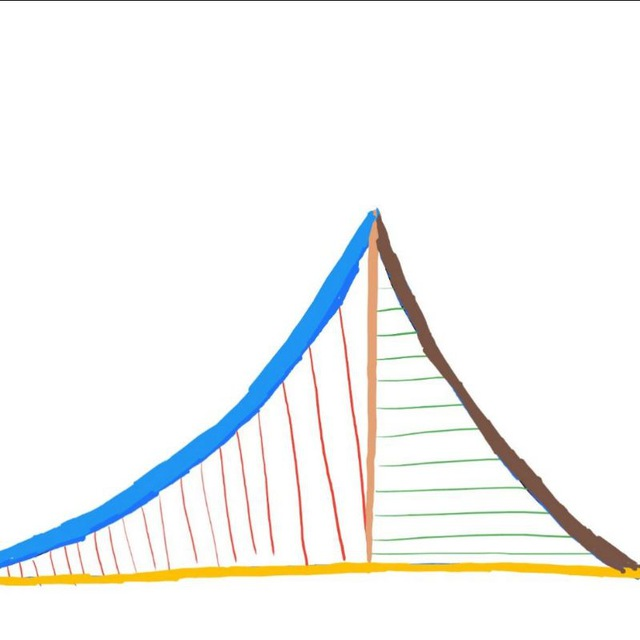
\includegraphics[width=0.2\columnwidth]{figs/logo.jpg}
\\
		{	\huge G. V. V. Sharma}
		\\
\vspace{1cm}
https://creativecommons.org/licenses/by-sa/3.0/
\\
and
\\
https://www.gnu.org/licenses/fdl-1.3.en.html
	\end{flushleft}
%\IEEEpubid{\makebox[\columnwidth]{978-1-7281-5966-1/20/\$31.00 ©2020 IEEE \hfill} \hspace{\columnsep}\makebox[\columnwidth]{ }}
}
\maketitle

\newpage


\tableofcontents

\newpage
\twocolumn


\renewcommand{\thefigure}{\theenumi}
\renewcommand{\thetable}{\theenumi}
%\renewcommand{\theequation}{\theenumi}


\section{Vectors}
%\numberwithin{equation}{section}
Consider a triangle with vertices
		\begin{align}
			\label{eq:tri-pts}
			\vec{A} = \myvec{1 \\ -1},\,
			\vec{B} = \myvec{-4 \\ 6},\,
			\vec{C} = \myvec{-3 \\ -5}
		\end{align}
\subsection{Sides}
%\renewcommand{\theequation}{\theenumi}
\begin{enumerate}[label=\thesubsection.\arabic*.,ref=\thesubsection.\theenumi]
\numberwithin{equation}{enumi}
\item The direction vector of $AB$ is defined as
		\begin{align}
			\vec{B}-
			\vec{A}
		\end{align}
Find the direction vectors of $AB, BC$ and $CA$.
\\
\solution 
\begin{enumerate} 
\item  The Direction vector of $AB$ is 
	\begin{align}  \vec{B} - \vec{A} 
		=\myvec{ -4\\ 6 } - \myvec{ 1\\ -1 }
 = \myvec{ -4 - 1\\ 6 - (-1) } = \myvec{ -5\\ 7 }
		\label{eq:geo-dir-vec-ab}
 \end{align}
\item The Direction vector of $BC$ is
	\begin{align} \vec{C} - \vec{B}=\myvec{ -3\\ -5} - \myvec{ -4\\ 6 }
 = \myvec{ -3 - (-4)\\ -5 - 6 } = \myvec{1\\ -11 }
		\label{eq:geo-dir-vec-bc}
  \end{align}
  \item  The Direction vector of $CA$  is
	  \begin{align}  \vec{A} - \vec{C} =\myvec{ 1\\ -1 }-\myvec{ -3\\ -5}
 = \myvec{ 1 - (-3)\\ -1 - (-5) } = \myvec{ 4\\ 4 }
		\label{eq:geo-dir-vec-ca}
  \end{align}
 \end{enumerate}
%	\solution 
\begin{enumerate} 
\item  The Direction vector of $AB$ is 
	\begin{align}  \vec{B} - \vec{A} 
		=\myvec{ -4\\ 6 } - \myvec{ 1\\ -1 }
 = \myvec{ -4 - 1\\ 6 - (-1) } = \myvec{ -5\\ 7 }
		\label{eq:geo-dir-vec-ab}
 \end{align}
\item The Direction vector of $BC$ is
	\begin{align} \vec{C} - \vec{B}=\myvec{ -3\\ -5} - \myvec{ -4\\ 6 }
 = \myvec{ -3 - (-4)\\ -5 - 6 } = \myvec{1\\ -11 }
		\label{eq:geo-dir-vec-bc}
  \end{align}
  \item  The Direction vector of $CA$  is
	  \begin{align}  \vec{A} - \vec{C} =\myvec{ 1\\ -1 }-\myvec{ -3\\ -5}
 = \myvec{ 1 - (-3)\\ -1 - (-5) } = \myvec{ 4\\ 4 }
		\label{eq:geo-dir-vec-ca}
  \end{align}
 \end{enumerate}


	\item The length of side $BC$ is 
		\label{prob:side-length}
		\begin{align}
			c = \norm{\vec{B}-\vec{A}} \triangleq \sqrt{\brak{\vec{B}-\vec{A}}^{\top}\brak{\vec{B}-\vec{A}}}
		\end{align}
		where
		\begin{align}
			\vec{A}^{\top}\triangleq\myvec{1 & -1}
		\end{align}
		Similarly, 
		\begin{align}
b = \norm{\vec{C}-\vec{B}},\,
a = \norm{\vec{A}-\vec{C}}
		\end{align}
		Find $a, b, c$.
\begin{enumerate}
	\item 
	From 	
		\eqref{eq:geo-dir-vec-ab},
\begin{align}
\vec{A}-\vec{B} &= \myvec{5\\-7}, \\
\implies 	c &= 	\norm{\vec{B}-\vec{A}} = \norm{\vec{A}-\vec{B}} 
	\\
	&= \sqrt{\myvec{5 & -7}\myvec{5\\-7}}
= \sqrt{\brak{5}^2 +\brak{7}^2}\\
	&=\sqrt{74}
		\label{eq:geo-norm-ab}
\end{align}
	\item Similarly, from 
		\eqref{eq:geo-dir-vec-bc},
\begin{align}
	a &= \norm{\vec{B}-\vec{C}} 
	= \sqrt{\myvec{-1 & 11}\myvec{-1\\11}}
\\
&= \sqrt{\brak{1}^2+\brak{11}^2}
	= \sqrt{122}
		\label{eq:geo-norm-bc}
\end{align}
and
		from 		\eqref{eq:geo-dir-vec-ca},
	\item 
		\begin{align}
			b &= \norm{\vec{A}-\vec{C}} = \sqrt{\myvec{4 & 4}\myvec{4\\4}}
\\
&= \sqrt{\brak{4}^2+\brak{4}^2}
	=\sqrt{32}
		\label{eq:geo-norm-ca}
\end{align}
\end{enumerate}
%  \\            
  %\begin{enumerate}
	\item Since,
\begin{align}
\vec{A}-\vec{B} &= \myvec{5\\-7}, \\
c = 	\norm{\vec{A}-\vec{B}} &= \sqrt{\myvec{5 & -7}\myvec{5\\-7}}
= \sqrt{\brak{5}^2 +\brak{7}^2}\\
	&=\sqrt{74}
		\label{eq:geo-norm-ab}
\end{align}
	\item Similarly, 
\begin{align}
\vec{B}-\vec{C} &= \myvec{-1\\11}\\
\implies 
a = \norm{\vec{B}-\vec{C}} &= \sqrt{\myvec{-1 & 11}\myvec{-1\\11}}
= \sqrt{\brak{1}^2+\brak{11}^2}
\\
	&= \sqrt{122}
		\label{eq:geo-norm-bc}
\end{align}
and
	\item \begin{align}
\vec{A}-\vec{C} &= \myvec{4\\4}\\
\implies
b = \norm{\vec{A}-\vec{C}} &= \sqrt{\myvec{4 & 4}\myvec{4\\4}}
= \sqrt{\brak{4}^2+\brak{4}^2}
\\
	&=\sqrt{32}
		\label{eq:geo-norm-ca}
\end{align}
\end{enumerate}

\item   Points $\vec{A}, \vec{B}, \vec{C}$ are defined to be collinear if 
		\begin{align}
			\label{eq:line-rank}
			\rank{\myvec{1 & 1 & 1 \\ \vec{A}& \vec{B}&\vec{C}}} = 2
		\end{align}
Are the given points in
			\eqref{eq:tri-pts}
collinear?
\\
\solution 
From 
			\eqref{eq:tri-pts},
\begin{align}
    \label{eq:1.1.3,2}
\myvec{
    1 & 1 & 1\\
    \vec{A} & \vec{B} & \vec{C} \\
    } 
    =
    %\label{eq:matthrowoperations}
    \myvec{
    1 & 1 & 1
    \\
    1 & -4 & -3
    \\
    -1 & 6 & -5
    }
     \xleftrightarrow[]{R_3 \leftarrow R_3+R_2}
    \myvec{
    1 & 1 & 1
    \\
    1 & -4 & -3
    \\
    0 & 2 & -8 
    }
    \\
     \xleftrightarrow[]{R_2\leftarrow R_1-R_2}
    \myvec{
    1 & 1 & 1
    \\
    0 & 5 & 4
    \\
    0 & 2 & -8 
    }
     \xleftrightarrow[]{R_3\leftarrow R_3-\frac{2}{5}R_2}
    \myvec{
    1 & 1 & 1
    \\
    0 & 5 & 4
    \\
    0 & 0 & \frac{-48}{5}
    }
\end{align}
There are no zero rows. So,
\begin{align}
    \text{rank}\myvec{
    1 & 1 & 1\\
    \vec{A} & \vec{B} & \vec{C} \\
    } &= 3 
\end{align}  
Hence,  the points $\vec{A},\vec{B},\vec{C}$ are not collinear. 
This is visible in 
\figref{fig1:Triangle}.
\begin{figure}[h]
\centering
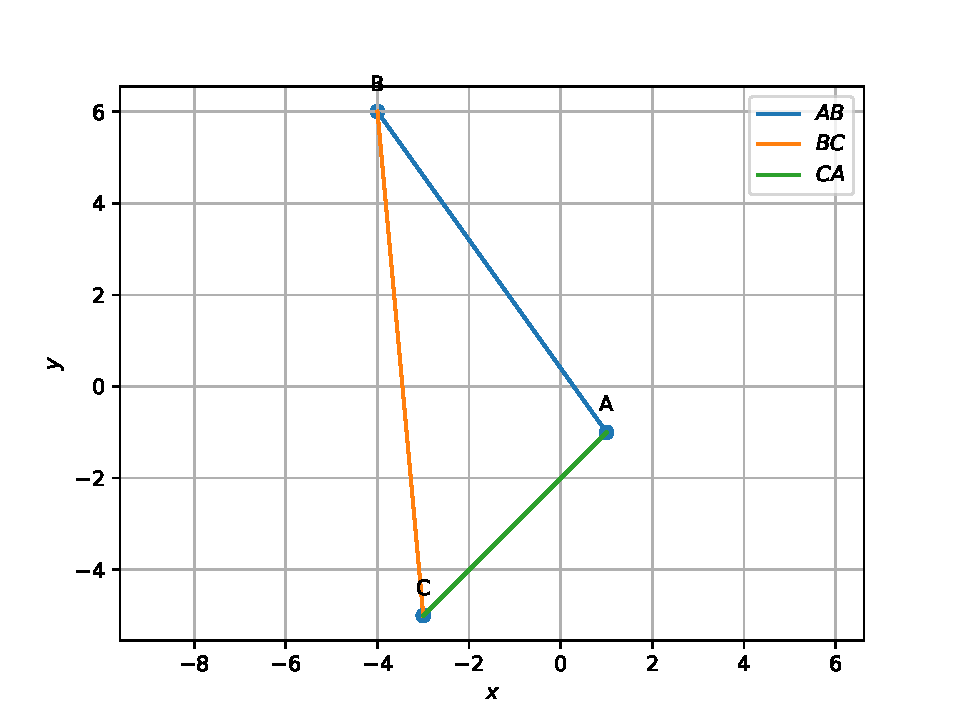
\includegraphics[width=\columnwidth]{figs/triangle/vector.pdf}
\caption{$\triangle ABC$}
\label{fig1:Triangle}
\end{figure}
% \\		\solution 
From 
			\eqref{eq:tri-pts},
\begin{align}
    \label{eq:1.1.3,2}
\myvec{
    1 & 1 & 1\\
    \vec{A} & \vec{B} & \vec{C} \\
    } 
    =
    %\label{eq:matthrowoperations}
    \myvec{
    1 & 1 & 1
    \\
    1 & -4 & -3
    \\
    -1 & 6 & -5
    }
     \xleftrightarrow[]{R_3 \leftarrow R_3+R_2}
    \myvec{
    1 & 1 & 1
    \\
    1 & -4 & -3
    \\
    0 & 2 & -8 
    }
    \\
     \xleftrightarrow[]{R_2\leftarrow R_1-R_2}
    \myvec{
    1 & 1 & 1
    \\
    0 & 5 & 4
    \\
    0 & 2 & -8 
    }
     \xleftrightarrow[]{R_3\leftarrow R_3-\frac{2}{5}R_2}
    \myvec{
    1 & 1 & 1
    \\
    0 & 5 & 4
    \\
    0 & 0 & \frac{-48}{5}
    }
\end{align}
There are no zero rows. So,
\begin{align}
    \text{rank}\myvec{
    1 & 1 & 1\\
    \vec{A} & \vec{B} & \vec{C} \\
    } &= 3 
\end{align}  
Hence,  the points $\vec{A},\vec{B},\vec{C}$ are not collinear. 
This is visible in 
\figref{fig1:Triangle}.
\begin{figure}[h]
\centering
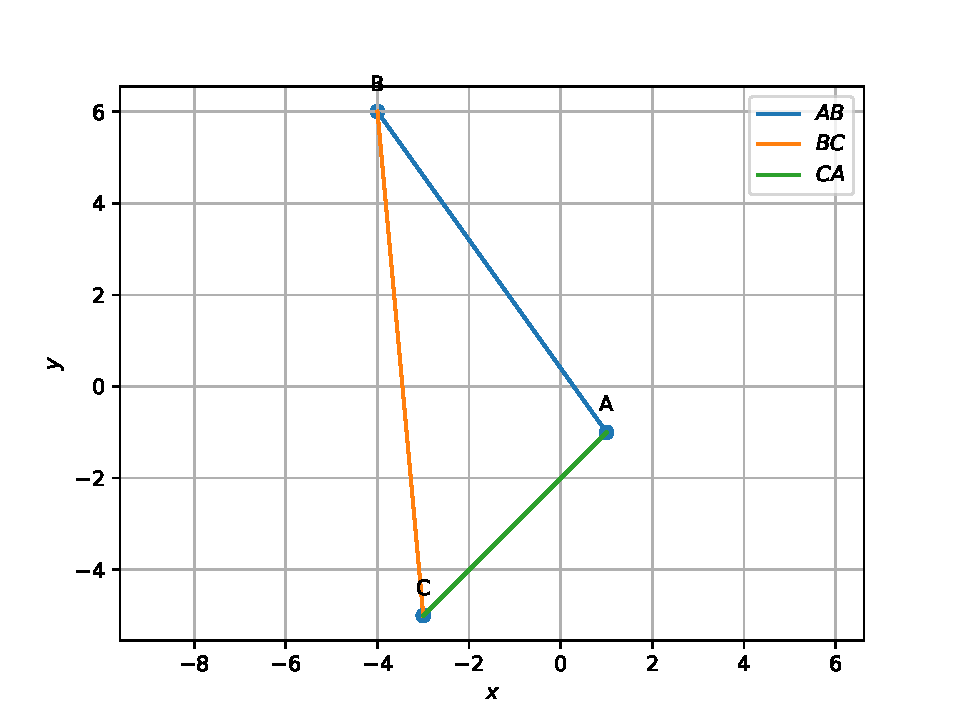
\includegraphics[width=\columnwidth]{figs/triangle/vector.pdf}
\caption{$\triangle ABC$}
\label{fig1:Triangle}
\end{figure}

\item The parameteric form of the equation  of $AB$ is 
		\begin{align}
			\label{eq:geo-param}
			\vec{x}=\vec{A}+k\vec{m} \quad k \ne 0,
		\end{align}
		where
		\begin{align}
\vec{m}=\vec{B}-\vec{A}
		\end{align}
is the direction vector of $AB$.
Find the parameteric equations of $AB, BC$ and $CA$.
\\
\solution
From 
			\eqref{eq:geo-param} and
		\eqref{eq:geo-dir-vec-ab},
the parametric equation for $AB$ is given by
\begin{align}
AB: \vec{x} = &\myvec{1\\-1} + k \myvec{-5\\7}
\end{align}
Similarly, from 
		\eqref{eq:geo-dir-vec-bc} and
		\eqref{eq:geo-dir-vec-ca},
\begin{align}
BC: \vec{x} = &\myvec{-4\\6} + k \myvec{1\\-11}\\
CA: \vec{x} = &\myvec{-3\\-5} + k \myvec{4\\4}
\end{align}

%		\solution
From 
			\eqref{eq:geo-param} and
		\eqref{eq:geo-dir-vec-ab},
the parametric equation for $AB$ is given by
\begin{align}
AB: \vec{x} = &\myvec{1\\-1} + k \myvec{-5\\7}
\end{align}
Similarly, from 
		\eqref{eq:geo-dir-vec-bc} and
		\eqref{eq:geo-dir-vec-ca},
\begin{align}
BC: \vec{x} = &\myvec{-4\\6} + k \myvec{1\\-11}\\
CA: \vec{x} = &\myvec{-3\\-5} + k \myvec{4\\4}
\end{align}


\item The normal form of the equation of $AB$  is 
		\begin{align}
			\label{eq:geo-normal}
			\vec{n}^{\top}\brak{	\vec{x}-\vec{A}} = 0
		\end{align}
		where 
		\begin{align}
			\vec{n}^{\top}\vec{m}&=\vec{n}^{\top}\brak{\vec{B}-\vec{A}} = 0
			\\
			\text{or, } \vec{n}&=\myvec{0 & 1 \\ -1 & 0} \vec{m}
			\label{eq:geo-norm-vec}
		\end{align}
Find the normal form of the equations of $AB, BC$ and $CA$.
\\
\solution
\begin{enumerate}
	\item
From
		\eqref{eq:geo-dir-vec-bc}, 
the direction vector of side $\vec{BC}$ is
\begin{align}
\vec{m}
	&=\myvec{1\\-11}
	\\
\implies \vec{n} &= \myvec{0 & 1\\
  -1 & 0}\myvec{1\\-11}
 = \myvec{-11\\-1}
		\label{eq:geo-norm-vec-bc}
\end{align}
from 
			\eqref{eq:geo-norm-vec}.
Hence, from 
			\eqref{eq:geo-normal},
the normal equation of side $BC$ is 
\begin{align}
	\vec{n}^{\top}\brak{	\vec{x}-\vec{B}} &= 0
			\\
\implies    \myvec{-11 & -1}\vec{x}&=\myvec{-11 & -1}\myvec{-4\\6}\\
    \implies
BC: \quad    \myvec{11 & 1}\vec{x}&=-38
\end{align}
\item Similarly, for $AB$,
from 
		\eqref{eq:geo-dir-vec-ab}, 
\begin{align}
	\vec{m} &= \myvec{-5\\7}
	\\
\implies        \vec{n} 
                &= \myvec{0&1\\-1&0}\myvec{-5\\7}
                = \myvec{7\\5}
		\label{eq:geo-norm-vec-ab}
\end{align}
and 
\begin{align}
	\vec{n}^{\top}\brak{	\vec{x}-\vec{A}} &= 0
	\\
	\implies
                AB: \quad  \vec{n}^{\top}\vec{x} &= \myvec{7&5}\myvec{1\\-1}\\    
       \implies\myvec{7&5}\vec{x} &= 2
\end{align}
\item For 
$CA$, 
from 
		\eqref{eq:geo-dir-vec-ca}, 
\begin{align}
\vec{m} &= \myvec{1 \\ 1}
\\
		\label{eq:geo-norm-vec-ca}
\implies \vec{n} 
&= \myvec{0&1 \\ -1&0}\myvec{1 \\ 1}
= \myvec{1 \\ -1}\\
\\
\implies	\vec{n}^{\top}\brak{	\vec{x}-\vec{C}} &= 0
\\
\implies \myvec{1&-1}{\vec{x}} &= \myvec{1&-1}\myvec{-3 \\ -5} 
= 2 
\end{align}
\end{enumerate}

%\begin{enumerate}
	\item
From
		\eqref{eq:geo-dir-vec-bc}, 
the direction vector of side $\vec{BC}$ is
\begin{align}
\vec{m}
	&=\myvec{1\\-11}
	\\
\implies \vec{n} &= \myvec{0 & 1\\
  -1 & 0}\myvec{1\\-11}
 = \myvec{-11\\-1}
		\label{eq:geo-norm-vec-bc}
\end{align}
from 
			\eqref{eq:geo-norm-vec}.
Hence, from 
			\eqref{eq:geo-normal},
the normal equation of side $BC$ is 
\begin{align}
	\vec{n}^{\top}\brak{	\vec{x}-\vec{B}} &= 0
			\\
\implies    \myvec{-11 & -1}\vec{x}&=\myvec{-11 & -1}\myvec{-4\\6}\\
    \implies
BC: \quad    \myvec{11 & 1}\vec{x}&=-38
\end{align}
\item Similarly, for $AB$,
from 
		\eqref{eq:geo-dir-vec-ab}, 
\begin{align}
	\vec{m} &= \myvec{-5\\7}
	\\
\implies        \vec{n} 
                &= \myvec{0&1\\-1&0}\myvec{-5\\7}
                = \myvec{7\\5}
		\label{eq:geo-norm-vec-ab}
\end{align}
and 
\begin{align}
	\vec{n}^{\top}\brak{	\vec{x}-\vec{A}} &= 0
	\\
	\implies
                AB: \quad  \vec{n}^{\top}\vec{x} &= \myvec{7&5}\myvec{1\\-1}\\    
       \implies\myvec{7&5}\vec{x} &= 2
\end{align}
\item For 
$CA$, 
from 
		\eqref{eq:geo-dir-vec-ca}, 
\begin{align}
\vec{m} &= \myvec{1 \\ 1}
\\
		\label{eq:geo-norm-vec-ca}
\implies \vec{n} 
&= \myvec{0&1 \\ -1&0}\myvec{1 \\ 1}
= \myvec{1 \\ -1}\\
\\
\implies	\vec{n}^{\top}\brak{	\vec{x}-\vec{C}} &= 0
\\
\implies \myvec{1&-1}{\vec{x}} &= \myvec{1&-1}\myvec{-3 \\ -5} 
= 2 
\end{align}
\end{enumerate}


\item The area of $\triangle ABC$ is defined as
		\begin{align}
			\label{eq:tri-area-cross}
			\frac{1}{2}\norm{{\brak{\vec{A}-\vec{B}}\times \brak{\vec{A}-\vec{C}}}}
		\end{align}
		where
		\begin{align}
			\vec{A}\times\vec{B} \triangleq \mydet{1 & -4 \\-1 & 6}
		\end{align}
		Find the area of $\triangle ABC$.\\
\solution
From
		\eqref{eq:geo-dir-vec-ab}
		and
		\eqref{eq:geo-dir-vec-ca},
\begin{align}
	\vec{A}-\vec{B}=\myvec{5\\-7},
	\vec{A}-\vec{C}&=\myvec{4\\4}\\
\implies (\vec{A}-\vec{B})\times(\vec{A}-\vec{C}) &=\mydet{5 & 4\\-7 & 4}\\
&=5\times 4-4\times (-7)\\&=48\\
\implies\frac{1}{2}\norm{(\vec{A}-\vec{B})\times(\vec{A}-\vec{C})}&=\frac{48}{2}=24
\end{align}
which is the desired area.

%  		\solution
From
		\eqref{eq:geo-dir-vec-ab}
		and
		\eqref{eq:geo-dir-vec-ca},
\begin{align}
	\vec{A}-\vec{B}=\myvec{5\\-7},
	\vec{A}-\vec{C}&=\myvec{4\\4}\\
\implies (\vec{A}-\vec{B})\times(\vec{A}-\vec{C}) &=\mydet{5 & 4\\-7 & 4}\\
&=5\times 4-4\times (-7)\\&=48\\
\implies\frac{1}{2}\norm{(\vec{A}-\vec{B})\times(\vec{A}-\vec{C})}&=\frac{48}{2}=24
\end{align}
which is the desired area.


	\item Find the angles $A, B, C$ if 
%    \label{prop:angle2d}
  \begin{align}
    \label{eq:angle2d}
			\cos A \triangleq 
\frac{\brak{\vec{B}-\vec{A}}^{\top}{\vec{C}-\vec{A}}}{\norm{\vec{B}-\vec{A}}\norm{\vec{C}-\vec{A}}}
  \end{align}\\
  \solution
\begin{enumerate}
	\item From 
		\eqref{eq:geo-dir-vec-ab},
		\eqref{eq:geo-dir-vec-ca},
		\eqref{eq:geo-norm-ab}
		and
		\eqref{eq:geo-norm-ca}
\begin{align}
	(\vec{B}-\vec{A})^{\top}(\vec{C}-\vec{A})&=\myvec{-5&7}\myvec{-4\\-4}\\
	&=-8
	\\
	\implies
	\cos{A}&= \frac{-8}{\sqrt{74} \sqrt{32}}
	= \frac{-1}{\sqrt{37}}\\
	\implies A&=\cos^{-1}{\frac{-1}{\sqrt{37}}}
\end{align}
	\item From 
		\eqref{eq:geo-dir-vec-ab},
		\eqref{eq:geo-dir-vec-bc},
		\eqref{eq:geo-norm-ab}
		and
		\eqref{eq:geo-norm-bc}
\begin{align}
	(\vec{C}-\vec{B})^{\top}(\vec{A}-\vec{B})&=\myvec{1&-11}\myvec{5\\-7}\\
	&= 82
	\\
	\implies
	\cos{B}&= \frac{82}{\sqrt{74} \sqrt{122}}
	= \frac{41}{\sqrt{2257}}\\
	\implies B&=\cos^{-1}{\frac{41}{\sqrt{2257}}}
\end{align}
	\item From 
		\eqref{eq:geo-dir-vec-bc},
		\eqref{eq:geo-dir-vec-ca},
		\eqref{eq:geo-norm-bc}
		and
		\eqref{eq:geo-norm-ca}
\begin{align}
	(\vec{A}-\vec{C})^{\top}(\vec{B}-\vec{C})&=\myvec{4&4}\myvec{-1\\11}\\
	&=40
	\\
\implies	\cos{C}&= \frac{40}{\sqrt{32} \sqrt{122}}
	= \frac{5}{\sqrt{61}}\\
	\implies C&=\cos^{-1}{\frac{5}{\sqrt{61}}}
\end{align}

\end{enumerate}
%  	\begin{enumerate}
	\item From 
		\eqref{eq:geo-dir-vec-ab},
		\eqref{eq:geo-dir-vec-ca},
		\eqref{eq:geo-norm-ab}
		and
		\eqref{eq:geo-norm-ca}
\begin{align}
	(\vec{B}-\vec{A})^{\top}(\vec{C}-\vec{A})&=\myvec{-5&7}\myvec{-4\\-4}\\
	&=-8
	\\
	\implies
	\cos{A}&= \frac{-8}{\sqrt{74} \sqrt{32}}
	= \frac{-1}{\sqrt{37}}\\
	\implies A&=\cos^{-1}{\frac{-1}{\sqrt{37}}}
\end{align}
	\item From 
		\eqref{eq:geo-dir-vec-ab},
		\eqref{eq:geo-dir-vec-bc},
		\eqref{eq:geo-norm-ab}
		and
		\eqref{eq:geo-norm-bc}
\begin{align}
	(\vec{C}-\vec{B})^{\top}(\vec{A}-\vec{B})&=\myvec{1&-11}\myvec{5\\-7}\\
	&= 82
	\\
	\implies
	\cos{B}&= \frac{82}{\sqrt{74} \sqrt{122}}
	= \frac{41}{\sqrt{2257}}\\
	\implies B&=\cos^{-1}{\frac{41}{\sqrt{2257}}}
\end{align}
	\item From 
		\eqref{eq:geo-dir-vec-bc},
		\eqref{eq:geo-dir-vec-ca},
		\eqref{eq:geo-norm-bc}
		and
		\eqref{eq:geo-norm-ca}
\begin{align}
	(\vec{A}-\vec{C})^{\top}(\vec{B}-\vec{C})&=\myvec{4&4}\myvec{-1\\11}\\
	&=40
	\\
\implies	\cos{C}&= \frac{40}{\sqrt{32} \sqrt{122}}
	= \frac{5}{\sqrt{61}}\\
	\implies C&=\cos^{-1}{\frac{5}{\sqrt{61}}}
\end{align}

\end{enumerate}

All codes for this section are available at
\begin{lstlisting}
	codes/triangle/sides.py
\end{lstlisting}
\end{enumerate}

\newpage
\subsection{Median}
\begin{enumerate}[label=\thesubsection.\arabic*.,ref=\thesubsection.\theenumi]
\numberwithin{equation}{enumi}
\item If $\vec{D}$ divides $BC$ in the ratio $k : 1$,
		\begin{align}
			\vec{D}= \frac{k\vec{C}+\vec{B}}{k+1}
	  \label{eq:section_formula}
		\end{align}
		Find the mid points $\vec{D}, \vec{E}, \vec{F}$ of the sides $BC, CA$ and $AB$ respectively.
	\\
		\solution
Since $\vec{D}$ is the midpoint of $BC$,
\begin{align}
k &= 1,\\
\implies \vec{D} &= \frac{\vec{C} + \vec{B}}{2}
= \frac{1}{2}\myvec{-7\\1}
	\label{eq:median-d}
\end{align}
Similarly,
\begin{align}
	\label{eq:median-e}
\vec{E} &= \frac{\vec{A} + \vec{C}}{2}
= \myvec{-1\\-3}\\
\vec{F} &= \frac{\vec{A} + \vec{B}}{2}
= \frac{1}{2}\myvec{-3\\5}
	\label{eq:median-f}
\end{align}
  
	\item Find the equations of $AD, BE$ and $CF$.
	\\	\\ \solution:
\begin{enumerate}
 \item The direction vector of $AD$ is 
\begin{align}
	\vec{m} = \vec{D}- \vec{A}
&=\myvec{\frac{-7}{2}\\\frac{1}{2}} - \myvec{1\\-1}
	=\frac{1}{2}\myvec{-9\\3} \equiv \myvec{-3 \\ 1}
	\\
	\implies  \vec{n} &=\myvec{1 \\ 3}
\end{align}
Hence the normal equation of median $AD$ is 
\begin{align}
\vec{n}^{\top}\myvec{\vec{x}-\vec{A}}&=0\\
\implies    \myvec{1 & 3}\vec{x}&=\myvec{1 & 3}\myvec{1\\-1}
    =-2
	\label{eq:median-ad}
\end{align}
\item For $BE$,
\begin{align}
	\vec{m}= \vec{E}- \vec{B}&=\myvec{-1\\-3} - \myvec{-4\\6}
       =\myvec{3\\-9}
       \equiv \myvec{1\\-3}
       \\
\implies 	
\vec{n} &= 
         \myvec{3\\1}
\end{align}
Hence the normal equation of median $BE$ is 
\begin{align}
\vec{n}^{\top}\myvec{\vec{x}-\vec{B}}&=0\\
\implies
	\myvec{3 & 1}   \vec{x}&=\myvec{3 &1}\myvec{-4\\6}
    =-6
	\label{eq:median-be}
\end{align}
\item For median $CF$,
\begin{align}
	\vec{m} = \vec{F}- \vec{C} &=
\myvec{\frac{-3}{2}\\\frac{5}{2}} - \myvec{-3\\-5}
       =\myvec{\frac{3}{2}\\\frac{15}{2}}
       \equiv \myvec{1 \\ 5}
       \\
	\implies \vec{n} &=\myvec{5 \\ -1}
\end{align}
Hence the normal equation of median $CF$ is 
\begin{align}
\vec{n}^{\top}\myvec{\vec{x}-\vec{C}}&=0\\
	\implies \myvec{5 & -1}\vec{x}&=\myvec{5 & -1}\myvec{-3\\-5}
    =-10
	\label{eq:median-cf}
\end{align}
\end{enumerate}
\iffalse
\begin{figure}
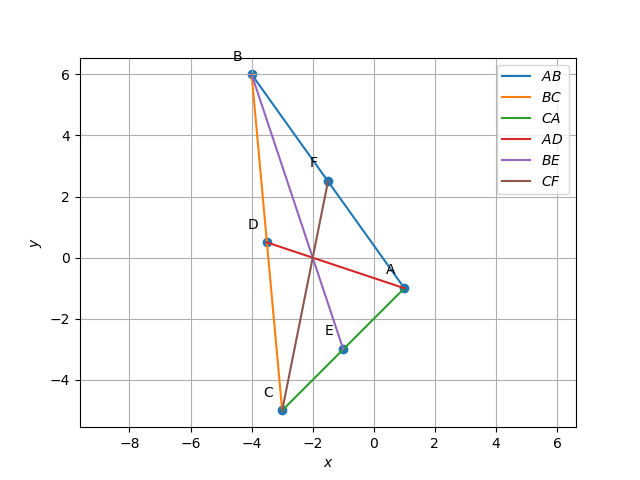
\includegraphics [width=\columnwidth] {solutions/1/2/2/figs/figure.png}
\caption{ Medians $AD$ , $BE$ and $CF$}
\label{fig: medians}
\end{figure}
\fi




% 		\iffalse
\let\negmedspace\undefined
\let\negthickspace\undefined
\documentclass[journal,12pt,twocolumn]{IEEEtran}
\usepackage{cite}
\usepackage{amsmath,amssymb,amsfonts,amsthm}
\usepackage{algorithmic}
\usepackage{graphicx}
\usepackage{textcomp}
\usepackage{xcolor}
\usepackage{txfonts}
\usepackage{listings}
\usepackage{enumitem}
\usepackage{mathtools}
\usepackage{gensymb}
\usepackage[breaklinks=true]{hyperref}
\usepackage{tkz-euclide} % loads  TikZ and tkz-base
\usepackage{listings}
\usepackage{gvv}
%
%\usepackage{setspace}
%\usepackage{gensymb}
%\doublespacing
%\singlespacing

%\usepackage{graphicx}
%\usepackage{amssymb}
%\usepackage{relsize}
%\usepackage[cmex10]{amsmath}
%\usepackage{amsthm}
%\interdisplaylinepenalty=2500
%\savesymbol{iint}
%\usepackage{txfonts}
%\restoresymbol{TXF}{iint}
%\usepackage{wasysym}
%\usepackage{amsthm}
%\usepackage{iithtlc}
%\usepackage{mathrsfs}
%\usepackage{txfonts}
%\usepackage{stfloats}
%\usepackage{bm}
%\usepackage{cite}
%\usepackage{cases}
%\usepackage{subfig}
%\usepackage{xtab}
%\usepackage{longtable}
%\usepackage{multirow}
%\usepackage{algorithm}
%\usepackage{algpseudocode}
%\usepackage{enumitem}
%\usepackage{mathtools}
%\usepackage{tikz}
%\usepackage{circuitikz}
%\usepackage{verbatim}
%\usepackage{tfrupee}
%\usepackage{stmaryrd}
%\usetkzobj{all}
%    \usepackage{color}                                            %%
%    \usepackage{array}                                            %%
%    \usepackage{longtable}                                        %%
%    \usepackage{calc}                                             %%
%    \usepackage{multirow}                                         %%
%    \usepackage{hhline}                                           %%
%    \usepackage{ifthen}                                           %%
  %optionally (for landscape tables embedded in another document): %%
%    \usepackage{lscape}     
%\usepackage{multicol}
%\usepackage{chngcntr}
%\usepackage{enumerate}

%\usepackage{wasysym}
%\documentclass[conference]{IEEEtran}
%\IEEEoverridecommandlockouts
% The preceding line is only needed to identify funding in the first footnote. If that is unneeded, please comment it out.

\newtheorem{theorem}{Theorem}[section]
\newtheorem{problem}{Problem}
\newtheorem{proposition}{Proposition}[section]
\newtheorem{lemma}{Lemma}[section]
\newtheorem{corollary}[theorem]{Corollary}
\newtheorem{example}{Example}[section]
\newtheorem{definition}[problem]{Definition}
%\newtheorem{thm}{Theorem}[section] 
%\newtheorem{defn}[thm]{Definition}
%\newtheorem{algorithm}{Algorithm}[section]
%\newtheorem{cor}{Corollary}
\newcommand{\BEQA}{\begin{eqnarray}}
\newcommand{\EEQA}{\end{eqnarray}}
\newcommand{\define}{\stackrel{\triangle}{=}}
\theoremstyle{remark}
\newtheorem{rem}{Remark}

%\bibliographystyle{ieeetr}
\begin{document}
%

\bibliographystyle{IEEEtran}


\vspace{3cm}

\title{ Solution of 1.2.2
%	\logo{

%	}
}
\author{ Dhruv Parashar$^{*}$% <-this % stops a space
	
}	
%\title{
%	\logo{Matrix Analysis through Octave}{\begin{center}\includegraphics[scale=.24]{tlc}\end{center}}{}{HAMDSP}
%}


% paper title
% can use linebreaks \\ within to get better formatting as desired
%\title{Matrix Analysis through Octave}
%
%
% author names and IEEE memberships
% note positions of commas and nonbreaking spaces ( ~ ) LaTeX will not break
% a structure at a ~ so this keeps an author's name from being broken across
% two lines.
% use \thanks{} to gain access to the first footnote area
% a separate \thanks must be used for each paragraph as LaTeX2e's \thanks
% was not built to handle multiple paragraphs
%

%\author{<-this % stops a space
%\thanks{}}
%}
% note the % following the last \IEEEmembership and also \thanks - 
% these prevent an unwanted space from occurring between the last author name
% and the end of the author line. i.e., if you had this:
% 
% \author{....lastname \thanks{...} \thanks{...} }
%                     ^------------^------------^----Do not want these spaces!
%
% a space would be appended to the last name and could cause every name on that
% line to be shifted left slightly. This is one of those "LaTeX things". For
% instance, "\textbf{A} \textbf{B}" will typeset as "A B" not "AB". To get
% "AB" then you have to do: "\textbf{A}\textbf{B}"
% \thanks is no different in this regard, so shield the last } of each \thanks
% that ends a line with a % and do not let a space in before the next \thanks.
% Spaces after \IEEEmembership other than the last one are OK (and needed) as
% you are supposed to have spaces between the names. For what it is worth,
% this is a minor point as most people would not even notice if the said evil
% space somehow managed to creep in.



% The paper headers
%\markboth{Journal of \LaTeX\ Class Files,~Vol.~6, No.~1, January~2007}%
%{Shell \MakeLowercase{\textit{et al.}}: Bare Demo of IEEEtran.cls for Journals}
% The only time the second header will appear is for the odd numbered pages
% after the title page when using the twoside option.
% 
% *** Note that you probably will NOT want to include the author's ***
% *** name in the headers of peer review papers.                   ***
% You can use \ifCLASSOPTIONpeerreview for conditional compilation here if
% you desire.




% If you want to put a publisher's ID mark on the page you can do it like
% this:
%\IEEEpubid{0000--0000/00\$00.00~\copyright~2007 IEEE}
% Remember, if you use this you must call \IEEEpubidadjcol in the second
% column for its text to clear the IEEEpubid mark.



% make the title area
\maketitle

\newpage

%\tableofcontents

\bigskip

\renewcommand{\thefigure}{\theenumi}
\renewcommand{\thetable}{\theenumi}
%\renewcommand{\theequation}{\theenumi}

%\begin{abstract}
%%\boldmath
%In this letter, an algorithm for evaluating the exact analytical bit error rate  (BER)  for the piecewise linear (PL) combiner for  multiple relays is presented. Previous results were available only for upto three relays. The algorithm is unique in the sense that  the actual mathematical expressions, that are prohibitively large, need not be explicitly obtained. The diversity gain due to multiple relays is shown through plots of the analytical BER, well supported by simulations. 
%
%\end{abstract}
% IEEEtran.cls defaults to using nonbold math in the Abstract.
% This preserves the distinction between vectors and scalars. However,
% if the journal you are submitting to favors bold math in the abstract,
% then you can use LaTeX's standard command \boldmath at the very start
% of the abstract to achieve this. Many IEEE journals frown on math
% in the abstract anyway.

% Note that keywords are not normally used for peerreview papers.
%\begin{IEEEkeywords}
%Cooperative diversity, decode and forward, piecewise linear
%\end{IEEEkeywords}



% For peer review papers, you can put extra information on the cover
% page as needed:
% \ifCLASSOPTIONpeerreview
% \begin{center} \bfseries EDICS Category: 3-BBND \end{center}
% \fi
%
% For peerreview papers, this IEEEtran command inserts a page break and
% creates the second title. It will be ignored for other modes.
%\IEEEpeerreviewmaketitle


Question:- 
We are given the three vertices of a triangle$(A,B,C)$ and the midpoints $\vec{D},\vec{E},\vec{F}$ of the sides $AB,BC,AC$ respectively. We have to find the equations of the sides $AD,BE,CF$.
\\
\fi
\solution
\begin{align}
\vec{A} &= \myvec{1\\-1} \\
\vec{B} &= \myvec{-4\\6} \\
\vec{C} &= \myvec{-3\\-5}
\end{align}
The mid points $\vec{D},\vec{E},\vec{F}$ of sides $AB,BC,AC$ are :-
\begin{align}
\vec{D} &= \frac{1}{2}\myvec{-7  \\ 1}\\
\vec{E} &= \myvec{-1\\-3}\\
\vec{F} &= \frac{1}{2}\myvec{-3  \\ 5}
\end{align}
Now, the direction vector of line $FC(\vec{m})$ is :-
\begin{align}
\vec{m} &= \vec{F} - \vec{C} \\
\implies \vec{m} &= \frac{1}{2}\myvec{3 \\ 15}
\end{align}
Now, we have to find $\vec{n}$,
\begin{align}
\vec{n} &= \myvec{0 & 1 \\ -1 & 0}\vec{m}\\
&= \frac{1}{2}\myvec{0 & 1 \\ -1 & 0}\myvec{3\\15}\\
&=\frac{1}{2}\myvec{15\\-3}
\end{align}
Normal form of line CF is :
\begin{align}
\vec{n}^{\top}(\vec{x-C}) &= 0\\
\vec{n}^{\top}\vec{x} &= \vec{n}^{\top}\vec{C} \\
\frac{1}{2}\myvec{15 & -3}\vec{x} &= \frac{1}{2}\myvec{15 & -3}\myvec{-3\\-5} \\
\myvec{15 & -3}\vec{x} &= \myvec{15 & -3}\myvec{-3\\-5} \\
\myvec{15 & -3}\vec{x} &= -30
\end{align}

\begin{figure}
\centering
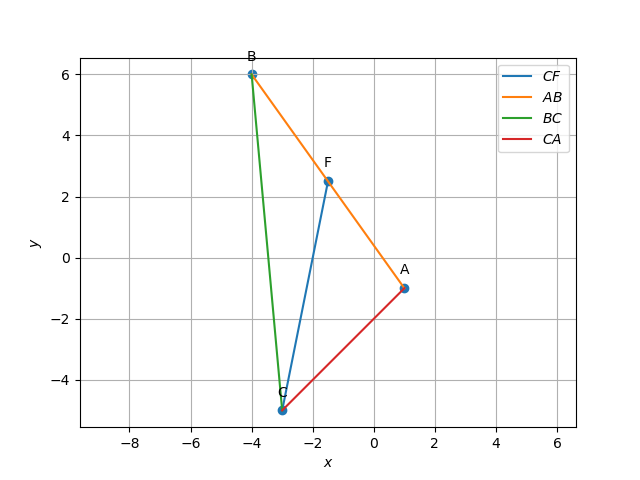
\includegraphics[width=\columnwidth]{solutions/1/2/2a/figs/figure.png}
\caption{Line CF}
\label{fig:Line CF}
\end{figure}



	\item Find the intersection $\vec{G}$ of $BE$ and $CF$.
 \\
\solution 
From 
	\eqref{eq:median-be}
	and
	\eqref{eq:median-cf},
the equations of $BE$ 
and 
$CF$
are, respectively,
\begin{align}
\myvec{3 & 1} \vec{x} &= \myvec{-6}
\label{eq:1.2.3,8}
\\
\myvec{ 5&-1} \vec{x} &= \myvec{-10}
\label{eq:1.2.3,9}
\end{align}
From \eqref{eq:1.2.3,8} and \eqref{eq:1.2.3,9} the augmented matrix is
\begin{align}
    \label{eq:matrowoperations}
    \myvec{
    3 & 1 & -6
    \\
    5 & -1 & -10
    }
     \xleftrightarrow[]{R_1 \leftarrow R_1+R_2}
    \myvec{
    8 & 0 & -16
    \\
    5 & -1 & -10 
    }
    \\
     \xleftrightarrow[]{R_1\leftarrow R_1/8}
    \myvec{
    1 & 0 & -2
    \\
    5 & -1 & -10 
    }
     \xleftrightarrow[]{R_2\leftarrow R_2-5R_1}
    \myvec{
    1 & 0 & -2
    \\
    0 & -1 & 0
    }
    \\
     \xleftrightarrow[]{R_2\leftarrow -R_2}
    \myvec{
    1 & 0 & -2
    \\
    0 & 1 & 0
    }
\end{align} 
using Gauss elimination.  Therefore, 
\begin{align}
\vec{G} = \myvec{-2 \\ 0}
	\label{eq:median-g}
\end{align}

	\item Verify that 
		\begin{align}
			\frac{BG}{GE} = 
			\frac{CG}{GF} =
			\frac{AG}{GD} =2 
		\end{align}
		\\	\solution 
\begin{enumerate}
\item From 
	\eqref{eq:median-e}
	and
	\eqref{eq:median-g},
\begin{align}
		\label{eq:tri-pts/4} \vec{G}-\vec{B} &= \myvec{2 \\ -6},\, 
 \vec{E}-\vec{G} = \myvec{1 \\ -3} \\
	\implies \vec{G}-\vec{B} &= 2 \brak{ \vec{E}-\vec{G} }
	\\
	\implies \norm{\vec{G}-\vec{B}} &= 2 \norm{ \vec{E}-\vec{G} }
	\\
	\text{or, }		\label{eq:tri-pts/8}\frac{BG}{GE} &=  2  
\end{align}		
\item From 
	\eqref{eq:median-f}
	and
	\eqref{eq:median-g},
\begin{align}
		 \vec{F}-\vec{G} &= \frac{1}{2}\myvec{ 1 \\ 5},\, 
 \vec{G}-\vec{C} &= \myvec{1 \\ 5} \\
	\implies 		 \vec{G}-\vec{C} &= 2 \brak{\vec{F}-\vec{G}} 
	\\
	\implies 		 \norm{\vec{G}-\vec{C}} &= 2 \norm{\vec{F}-\vec{G}} 
	\\
		\text{or, }	\frac{CG}{GF} &=  2		
\label{eq:tri-pts/9}
\end{align}
\item From
	\eqref{eq:median-d}
	and
	\eqref{eq:median-g},
\begin{align}
		\label{eq:tri-pts/14} \vec{G}-\vec{A} &= \myvec{-3 \\ 1} ,\,
 \vec{D}-\vec{G} = \frac{1}{2}\myvec{ -3 \\ 1}
 \\
	\vec{G}-\vec{A} &= 
	2\brak{ \vec{D}-\vec{G} } 
	\\
\implies		 \norm{\vec{G}-\vec{A}} &= 
 2\norm{\vec{D}-\vec{G}} 
 \\
		\text{or, }		\label{eq:tri-pts/18}\frac{AG}{GD} &=   2		
\end{align}
\end{enumerate}
From \eqref{eq:tri-pts/8}, \eqref{eq:tri-pts/9}, \eqref{eq:tri-pts/18}
\begin{align}
		\frac{BG}{GE} = 
		\frac{CG}{GF} =
		\frac{AG}{GD} = 2
\end{align}

	\item Show that $\vec{A}, \vec{G}$ and $\vec{D}$ are collinear.
	\\
		\solution 
Points $\vec{A},\vec{D},\vec{G}$ are defined to be collinear if 
\begin{align}
    \text{rank}\myvec{
    1 & 1 & 1\\
    \vec{A} & \vec{D} & \vec{G} \\
    } = 2 
    \label{eq:mat_row_operations}
    \\
\implies    
    \myvec{
    1 & 1 & 1
    \\
    1 & -\frac{7}{2} & -2
    \\
    -1 & \frac{1}{2} & 0
    }
     \xleftrightarrow[]{R_3 \leftarrow R_3+R_2}
    \myvec{
    1 & 1 & 1
    \\
    1 & -\frac{7}{2} & -2
    \\
    0 & -3 & -2 
    }
    \\
     \xleftrightarrow[]{R_2\leftarrow R_2-R_1}
    \myvec{
    1 & 1 & 1
    \\
    0 & -\frac{9}{2} & -3
    \\
    0 & -3 & -2 
    }
     \xleftrightarrow[]{R_3\leftarrow R_3-\frac{2}{3}R_2}
    \myvec{
    1 & 1 & 1
    \\
    0 & -\frac{9}{2} & -3
    \\
    0 & 0 & 0
    }
\end{align}
Thus, the matrix 
    \eqref{eq:mat_row_operations}
    has rank 2 and the points are collinear.
    Thus, the medians of a triangle meet at the point $\vec{G}$.
See \figref{fig:Triangle-median}.
\begin{figure}
\centering
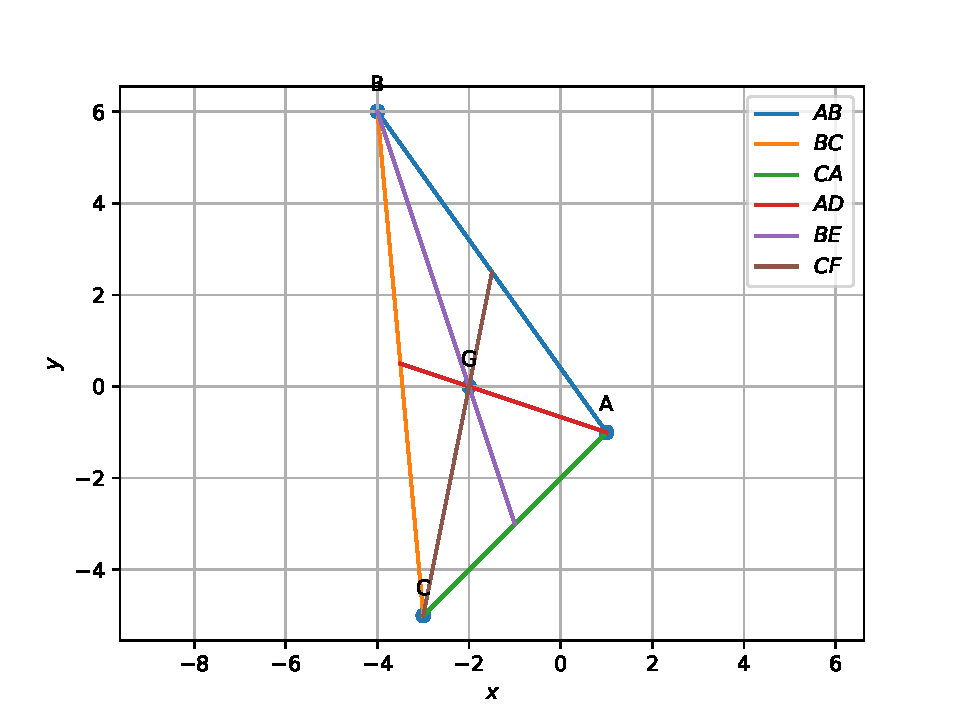
\includegraphics[width=\columnwidth]{figs/triangle/median.pdf}
	\caption{Medians of $\triangle ABC$ meet at $\vec{G}$.}
\label{fig:Triangle-median}
\end{figure}


	\item Verify that 
		\begin{align}
			\vec{G}=\frac{\vec{A}+\vec{B}+\vec{C}}{3}
		\end{align}
			$\vec{G}$ is known as the {\em centroid} of $\triangle ABC$.
   \\
		\solution
\begin{equation}
\begin{split}
\label{eq:centroid}
    \vec{G}&= \frac{\myvec{1\\-1}+\myvec{-4\\6}+\myvec{-3\\-5}}{3}\\    
     &= \myvec{-2\\0}
\end{split}
\end{equation}

 




	\item Verify that 
		\begin{align}
\vec{A}-\vec{F}=\vec{E}-\vec{D}
		\end{align}
		The quadrilateral $AFDE$ is defined to be a parallelogram.\\
  		\\ \solution 
\begin{align}
    \vec{A}-\vec{F}&=\myvec{1\\-1}-\myvec{\frac{-3}{2}\\\frac{5}{2}}
    =\myvec{\frac{5}{2}\\\frac{-7}{2}}
    \\
    \vec{E}-\vec{D}&=\myvec{-1\\-3}-\myvec{\frac{-7}{2}\\\frac{1}{2}}
    =\myvec{\frac{5}{2}\\\frac{-7}{2}}
    \\
	\implies	\vec{A}-\vec{F} &= \vec{E}-\vec{D}
\end{align}
See \figref{fig:Triangle-pgm}, 
\begin{figure}
\centering
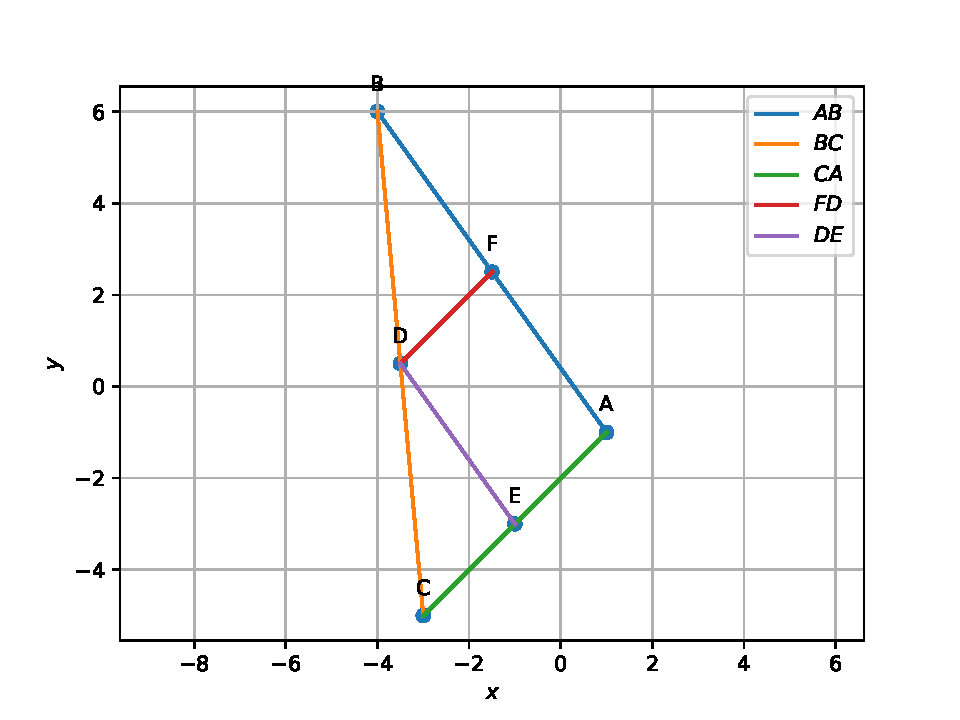
\includegraphics[width=\columnwidth]{figs/triangle/pgm.pdf}
\caption{$AFDE$ forms a parallelogram in triangle ABC}
\label{fig:Triangle-pgm}
\end{figure}






















All codes for this section are available in 
\begin{lstlisting}
	codes/triangle/medians.py
	codes/triangle/pgm.py
\end{lstlisting}
  
\end{enumerate}

\newpage
\subsection{Altitude}
\begin{enumerate}[label=\thesubsection.\arabic*.,ref=\thesubsection.\theenumi]
\numberwithin{equation}{enumi}
\numberwithin{figure}{enumi}
\item $\vec{D}_1$ is a point on $BC$ such that
		\begin{align}
			AD_1 \perp BC
		\end{align}
		and $AD_1$ is defined to be the altitude. 
		Find the normal vector of $AD_1$.
  \\
		\solution
The normal vector of $AD_{1}$ 
is
the direction vector $BC$ and is obtained from  
		\eqref{eq:geo-dir-vec-bc}
		as
\begin{align}
	\vec{n} = 
\myvec{1\\-11}
\end{align}


	\item Find the equation of $AD_1$.
 \\     \solution
The equation of $AD_1$ is
\begin{align}
 \vec{n}^{\top}(\vec{x-A}) &= 0 \\
\implies \myvec{-1 & 11}\vec{x} &= \myvec{-1 & 11}\myvec{1 \\ -1}
= -12
\end{align}


	\item Find the equations of the altitudes $BE_1$ and $CF_1$ to the sides $AC$ and $AB$ respectively. 
  \\     \\ \solution
\begin{enumerate}
\item 
	From 
		\eqref{eq:geo-dir-vec-ca},
the normal vector of $CF_1$ is 
\begin{align}
\vec{n}&=\myvec{-5\\7} 
\end{align}
and the equation of $CF_1$ is
\begin{align}
\vec{n}^{\top}\brak{\vec{x}-\vec{C}}&=0 \\
\implies 
\myvec{-5 & 7}\brak{\vec{x}-\myvec{-3\\-5}}&=0  \\
	\implies \myvec{5 & -7}\vec{x}&=20
		\label{eq:geo-alt-cf},
\end{align}
\item Similarly, 
	from 
		\eqref{eq:geo-dir-vec-ab},
the normal vector of $BE_1$ is 
\begin{align}
\vec{n}= \myvec{1 \\1}
\end{align}
and the equation of  $BE_1$ is
\begin{align}
\vec{n}^{\top}\brak{\vec{x}-\vec{B}}&=0 \\
	\implies \myvec{1 & 1}\brak{\vec{x}-\myvec{-4\\6}}&=0 \\
	\implies \myvec{1 & 1}\vec{x}&=2
		\label{eq:geo-alt-be},
\end{align}
\end{enumerate}



	\item Find the intersection $\vec{H}$ of $BE_1$ and $CF_1$.
 \\
        \\ \solution
%
The intersection of 
		\eqref{eq:app-geo-alt-be}
		and
		\eqref{eq:app-geo-alt-cf},
		is obtained from 
		the matrix equation
		%
\begin{align}
        \myvec{1&1\\5&-7} \vec{x} &= \myvec{2\\20}
\end{align}
%
which can be solved as 
%
\begin{align}
        \myvec{1&1&2\\5&-7&20}
	 \xleftrightarrow[]{R_2 \leftarrow R_2 - 5R_1}
        \myvec{1&1&2\\0&-12&10}\\
	 \xleftrightarrow[]{R_2 \leftarrow \frac{R_2}{-12}}
        \myvec{1&1&2\\0&1&\frac{-5}{6}}
	 \xleftrightarrow[]{R_1 \leftarrow R_1 - R_2}
        \myvec{1&0&\frac{17}{6}\\0&1&\frac{-5}{6}}
\end{align}
%
yielding
%
\begin{align}
        \vec{H}&=\frac{1}{6}\myvec{{17}\\-{5}}
		\label{eq:app-geo-alt-H},
\end{align}
%
See 
\figref{fig:m_tri_py}
\begin{figure}[H]
\centering
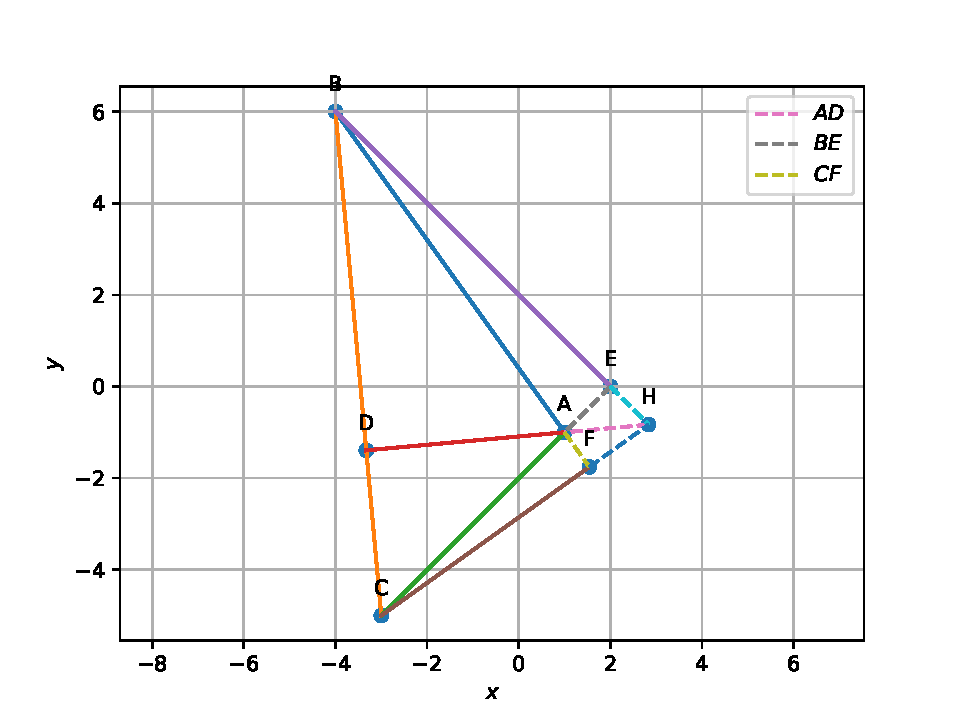
\includegraphics[width=0.75\columnwidth]{figs/triangle/altitude.pdf}
\caption{Altitudes $BE_1$ and $CF_1$ intersect at $\vec{H}$}
\label{fig:m_tri_py}
\end{figure}


	\item Verify that 
		\begin{align}
			\brak{\vec{A}-\vec{H}}^{\top}\brak{\vec{B}-\vec{C}} = 0
		\end{align}
  \solution
From 
		\eqref{eq:geo-alt-H},
\begin{align}
\vec{A}-\vec{H}=-\frac{1}{6}\myvec{{11}\\{1}},\,
\vec{B}-\vec{C}=\myvec{-1\\11}
\\
	\implies \brak{\vec{A}-\vec{H}}^{\top}\brak{\vec{B}-\vec{C}}=\frac{1}{6}\myvec{11 & 1}
\myvec{-1\\11}
=0
\end{align}


All codes for this section are available at
\begin{lstlisting}
	codes/triangle/altitude.py
\end{lstlisting}
\end{enumerate}

\newpage
\subsection{Perpendicular Bisector}
\begin{enumerate}[label=\thesubsection.\arabic*.,ref=\thesubsection.\theenumi]
\numberwithin{equation}{enumi}

\item The equation of the perpendicular bisector of $BC$ is
		\begin{align}
			\label{eq:tri-perp-bisect}
			\brak{\vec{x}-\frac{\vec{B}+\vec{C}}{2}}\brak{\vec{B}-\vec{C}} = 0
		\end{align}
		Substitute numerical values and find the equations of the perpendicular bisectors of $AB, BC$ and $CA$.
	\\	\solution
From 
		\eqref{eq:app-geo-dir-vec-ab},
		\eqref{eq:app-geo-dir-vec-bc},
		\eqref{eq:app-geo-dir-vec-ca},
	\eqref{eq:median-d},
	\eqref{eq:median-e}
	and
	\eqref{eq:median-f},
\begin{align}
\vec{\frac{\vec{B}+\vec{C}}{2}} &= \frac{1}{2}\myvec{-{7} \\ 1},\,
\vec{B}-\vec{C} = \myvec{-1 \\ 11} 
\\
\vec{\frac{\vec{A}+\vec{B}}{2}}&=\frac{1}{2}\myvec{-{3} \\{5}},\,
\vec{A}-\vec{B}=\myvec{5\\ -7} \\
\vec{\frac{\vec{C}+\vec{A}}{2}} &= \myvec{-1\\-3},\,
\vec{C}-\vec{A} = \myvec{-4\\-4} 
\end{align}
yielding
\begin{alignat}{2}
  \brak{\vec{B}-\vec{C}}^{\top}\brak{\frac{\vec{B}+\vec{C}}{2}}
	&=\myvec{-1&11}\myvec{-\frac{7}{2} \\ \frac{1}{2}}
	&&=9
  \\
\brak{\vec{A}-\vec{B}}^{\top}\brak{\frac{\vec{A}+\vec{B}}{2}}
	&=\myvec{5&-7}\myvec{-\frac{3}{2} \\\frac{5}{2}}
	&&=-25
  \\
\brak{\vec{C}-\vec{A}}^{\top}\brak{\frac{\vec{C}+\vec{A}}{2}}
	&=\myvec{-4&-4}\myvec{-1\\-3}
	&&=16
\end{alignat}
Thus, the perpendicular bisectors are obtained from 
			\eqref{eq:tri-perp-bisect}
			as
		\begin{alignat}{2}
			\label{eq:app-tri-perp-bisect-bc}
			BC&: \quad \myvec{-1&11}\vec{x}&&=9
\\
			\label{eq:app-tri-perp-bisect-ca}
			CA&: \quad \myvec{5&-7}\vec{x}&&=-25
\\
			\label{eq:app-tri-perp-bisect-ab}
			AB&: \quad \myvec{1&1}\vec{x}&&=-4
		\end{alignat}




	\item Find the intersection $\vec{O}$ of the perpendicular bisectors of $AB$ and $AC$.
 \\
 \solution \\
The intersection of 
			\eqref{eq:app-tri-perp-bisect-ca}
			and
			\eqref{eq:app-tri-perp-bisect-ab},
			can be obtained as
\begin{align}
\myvec{5&-7&-25\\1&1&-4} \xleftrightarrow[]{R_2 \leftarrow 5R_2 - R_1} \myvec{5&-7&-25\\0&12&5}\\
 \xleftrightarrow[]{R_1\leftarrow \frac{12}{7}R_1 + R_2} \myvec{\frac{60}{7}&0& \frac{-265}{7}\\0&12&5}
 \xleftrightarrow[R_1\leftarrow \frac{7}{60}R_1]{R_2 \leftarrow \frac{1}{12}R_2} \myvec{1&0& \frac{-53}{12}\\0&1&\frac{5}{12}}\\
\implies \vec{O}=\myvec{\frac{-53}{12}\\\frac{5}{12}}
			\label{eq:app-tri-perp-bisect-O}
\end{align}

	\item Verify that $\vec{O}$ satisfies
			\eqref{eq:tri-perp-bisect}.
$\vec{O}$ is known as the circumcentre.\\
    \solution
Substituing  from 
			\eqref{eq:tri-perp-bisect-O} in 
			\eqref{eq:tri-perp-bisect},
when substituted in the above equation,
\begin{multline}
	\brak{\vec{O}-\frac{\vec{B}+\vec{C}}{2}}^{\top}\brak{\vec{B}-\vec{C}}\\
	=\brak{\frac{1}{12}\myvec{-53\\5}- \frac{1}{2}\myvec{-7\\1}}^{\top} \myvec{-1\\11}\\
	=\frac{1}{12}\myvec{-11&-1}\myvec{-1\\11}
	=0
\end{multline}




		\item Verify that 
		\begin{align}
			OA = OB = OC 
		\end{align}
	\item Draw the circle with centre at $\vec{O}$ and radius 
		\begin{align}
			R = OA
		\end{align}
		This is known as the {\em circumradius}. 
  \\  \solution 
See 
\figref{fig:circumcircle with centre O}.
\begin{figure}
\centering
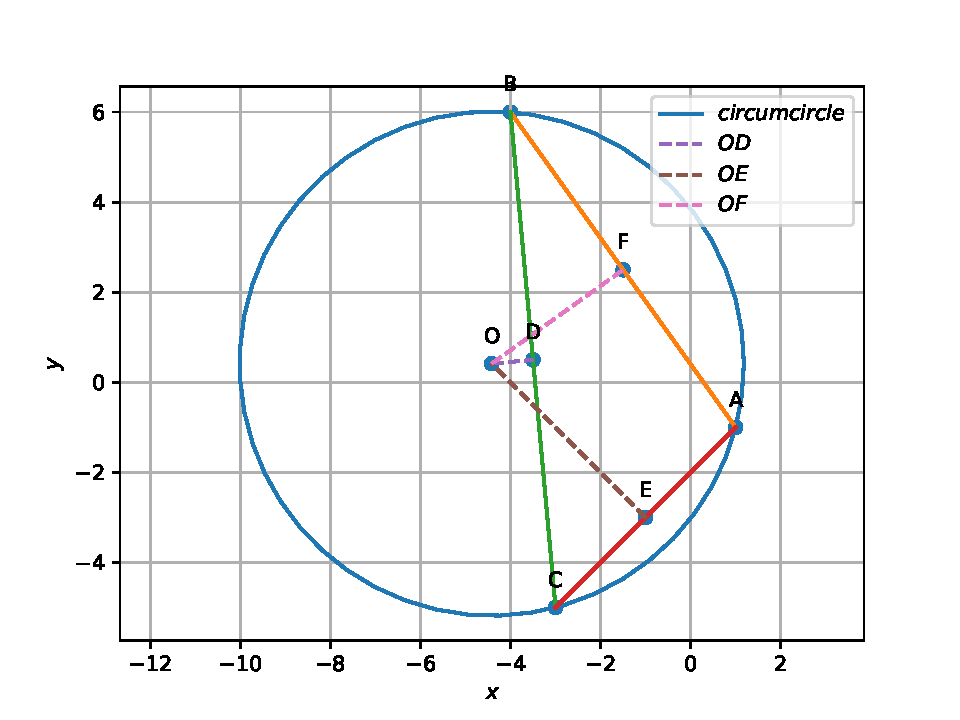
\includegraphics[width=0.75\columnwidth]{figs/triangle/perp-bisect.pdf}
	\caption{Circumcircle of $\triangle ABC$ with centre $\vec{O}$.}
\label{fig:circumcircle with centre O}	
\end{figure}


	\item Verify that 
		\begin{align}
			\angle BOC = 2\angle BAC.
		\end{align}\\
  \solution
\begin{enumerate}
\item To find  the value of $\angle{BOC}$ :
\begin{align}
\vec{B}-\vec{O}
          &=\myvec{\frac{5}{12}\\\frac{67}{12}},\,
\vec{C}-\vec{O}
          =\myvec{\frac{17}{12}\\\frac{-65}{12}}
	  \\
\implies \brak{\vec{B}-\vec{O}}^{\top}\brak{\vec{C}-\vec{O}}&=\frac{-4270}{144}\\
	\implies \norm{\vec{B}-\vec{O}}&= \frac{\sqrt{4514}}{12},\,
	\norm{\vec{C}-\vec{O}}= \frac{\sqrt{4514}}{12}
\end{align}
Thus,
\begin{align}
\cos{BOC}&=\frac{\brak{\vec{B}-\vec{O}}^{\top}\brak{\vec{C}-\vec{O}}}{\norm{\vec{B}-\vec{O}}\norm{\vec{C}-\vec{O}}}
=\frac{-4270}{4514}\\
\implies\angle{BOC}&=\cos^{-1}\brak{\frac{-4270}{4514}}
\\
	&=161.07536\degree
	\text{ or }
	198.92464\degree\label{eq:1}
\end{align}
	\item To find  the value of $\angle{BAC}$ :
\begin{align}
\vec{B}-\vec{A}&=\myvec{-5\\7},\,
\vec{C}-\vec{A}=\myvec{-4\\-4}
\\
\implies \brak{\vec{B}-\vec{A}}^{\top}\brak{\vec{C}-\vec{A}}&=-8
\\
	\norm{\vec{B}-\vec{A}}&= \sqrt{74}
	\norm{\vec{C}-\vec{A}}= 4\sqrt{2}
\end{align}
Thus,
\begin{align}
\cos{BAC}&=\frac{\brak{\vec{B}-\vec{A}}^{\top}\brak{\vec{C}-\vec{A}}}{\norm{\vec{B}-\vec{A}}\norm{\vec{C}-\vec{A}}}
=\frac{-8}{4\sqrt{148}}\\
\implies\angle{BAC}&=\cos^{-1}\brak{\frac{-8}{4\sqrt{148}}}\\
&=99.46232\degree \label{eq:2}
\end{align}
From \eqref{eq:2} and \eqref{eq:1},
\begin{align}
2\times\angle{BAC}
= \angle{BOC}
\end{align}
\end{enumerate}





	\item Let 
		\begin{align}
			\vec{P} = \myvec{\cos \theta & -\sin \theta \\ \sin \theta & \cos \theta}
		\end{align}
			where
\begin{align}
	\theta = \angle BOC
\end{align}
Verify that 
		\begin{align}
			\vec{B}-\vec{O}=\vec{P}\brak{\vec{C}-\vec{O}}
		\end{align}
All codes for this section are available at
\begin{lstlisting}
	codes/triangle/perp-bisect.py
\end{lstlisting}
\end{enumerate}

\newpage
\subsection{Angle Bisector}
\begin{enumerate}[label=\thesubsection.\arabic*.,ref=\thesubsection.\theenumi]
\numberwithin{equation}{enumi}
\numberwithin{figure}{enumi}
	\item Let $\vec{D}_3, \vec{E}_3, \vec{F}_3$, be points on $AB, BC$ and $CA$ respectively such that
		\begin{align}
			BD_3 = BF_3=m, CD_3 = CE_3=n, AE_3 = AF_3=p.
		\end{align}
	Obtain $m,n,p$ in terms of $a,b,c$ obtained in  
		\probref{prob:side-length}.
 \\
 		\solution 
From the given information, 
\begin{align}
% 
    a &= m+n,\\
    b &= n+p, \\
    c &= m+p 
\end{align}
which can be expressed as
\begin{align}
\myvec{1&1&0\\0&1&1\\1&0&1\\}\myvec{m\\n\\p} &= \myvec{a\\b\\c}
\\
\implies 
	\myvec{m\\n\\p} &= \myvec{1&1&0\\0&1&1\\1&0&1\\}^{-1}\myvec{a\\b\\c}
\end{align}
Using row reduction,
		\begin{align}
			\augvec{3}{3}{1&1&0 & 1 & 0 & 0\\0&1&1 & 0 & 1 & 0\\1&0&1 & 0 & 0 & 1}
			\\
			\xleftrightarrow[]{R_3 \leftarrow R_3 - R_1}
			\augvec{3}{3}{1&1&0 & 1 & 0 & 0\\0&1&1 & 0 & 1 & 0\\0&-1&1 & -1 & 0 & 1}
			\\
			\xleftrightarrow[R_1 \leftarrow R_1 - R_2]{R_3 \leftarrow R_3 + R_2}
			\augvec{3}{3}{1&0&-1 & 1 & -1 & 0\\0&1&1 & 0 & 1 & 0\\0&0&2 & -1 & 1 & 1}
		\end{align}
		\begin{align}
			\xleftrightarrow[R_1 \leftarrow 2R_1 + R_3]{R_2 \leftarrow 2R_2 - R_3}
			\augvec{3}{3}{2&0&0 & 1 & -1 & 1\\0&2&0 & 1 & 1 & -1\\0&0&2 & -1 & 1 & 1}
		\end{align}
yielding
		\begin{align}
			\myvec{1&1&0\\0&1&1\\1&0&1\\}^{-1} = 
			\frac{1}{2}\myvec{1 & -1 & 1\\ 1 & 1 & -1\\ -1 & 1 & 1}
		\end{align}
	Therefore,
\begin{align}
\begin{split}
    p&=\frac{c+b-a}{2}
    =\frac{\sqrt{74}+\sqrt{32}-\sqrt{122}}{2}
    \\
    m&=\frac{a+c-b}{2}
    =\frac{\sqrt{74}+\sqrt{122}-\sqrt{32}}{2}
    \\
    n&=\frac{a+b-c}{2}
    =\frac{\sqrt{122}+\sqrt{32}-\sqrt{74}}{2}
\end{split}
	\label{eq:incircle-mnp}
\end{align}
upon substituting from 
		\eqref{eq:geo-norm-ab},
		\eqref{eq:geo-norm-bc}
		and
		\eqref{eq:geo-norm-ca}.

	\item Using section formula, find 
		\begin{align}
			\vec{D}_3 = \frac{m\vec{C}+n\vec{B}}{m+n},\,
			\vec{E}_3 = \frac{n\vec{A}+p\vec{C}}{n+p},\,
			\vec{F}_3 = \frac{p\vec{B}+m\vec{A}}{p+m}
		\end{align}
	\item Find the circumcentre and circumradius of $\triangle D_3E_3F_3$.  These are the {\em incentre} and {\em inradius} of $\triangle ABC$.
	\item Draw the circumcircle of $\triangle D_3E_3F_3$.  This is known as the {\em incircle} of $\triangle ABC$.
		\\
 		\solution
See 
	\figref{fig:incircle}
\begin{figure}[!ht]
	\centering
	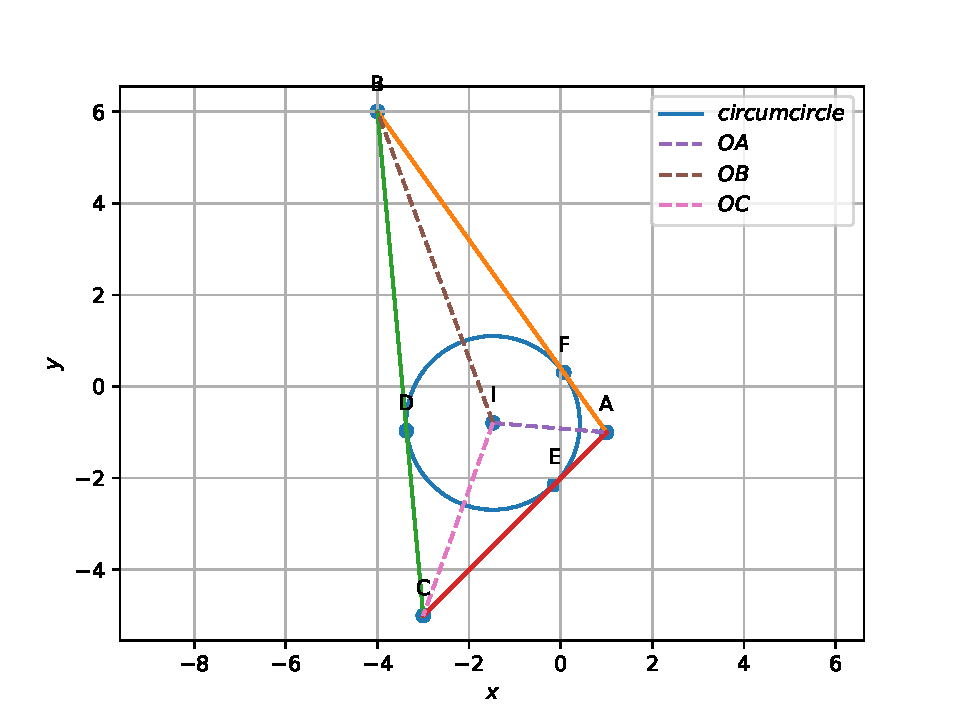
\includegraphics[width=\columnwidth]{figs/triangle/ang-bisect.pdf}
	\caption{Incircle of $\triangle ABC$}
	\label{fig:incircle}
\end{figure}
\iffalse
Considering
\begin{align}
	BC: \quad \vec{n} ^\top \vec{x} &= c, 
\end{align}
the distance from $\vec{I}$ to $BC$ is 
\begin{align}
\frac{\abs{\vec{n}^\top \vec{I} - c}}{\norm{\vec{n}}} 
\end{align}
\fi


	\item Using 
    \eqref{eq:app-angle2d}
verify that 
		\begin{align}
			\angle BAI = \angle CAI.
		\end{align}
		$AI$ is the bisector of $\angle A$.  
	\item Verify that $BI, CI$ are also the angle bisectors of $\triangle ABC$.
All codes for this section are available at
\begin{lstlisting}
	codes/triangle/ang-bisect.py
\end{lstlisting}

\end{enumerate}

\newpage
\subsection{Eigenvalues and Eigenvectors}
\begin{enumerate}[label=\thesubsection.\arabic*.,ref=\thesubsection.\theenumi]
\item 
	 The equation of a circle is given by 
	\label{prop:circ-eq}
\begin{align}
	\norm{\vec{x}}^2 + 2 \vec{u}^{\top}\vec{x} + f = 0
	\label{eq:circ-eq}
\end{align}
for
		\begin{align}
			 \label{eq:conic_quad_form-params}
	 \vec{u}=-\vec{O}, f = \norm{\vec{O}}-r^2,
		\end{align}
		$\vec{O}$ being the incentre and $r$ the inradius.  
\item Compute 
\begin{align}
	\label{eq:incircle-disc-Sigma}
\vec{\Sigma} = 
\brak{\vec{V}\vec{h}+\vec{u}}
	  \brak{\vec{V}\vec{h}+\vec{u}}^{\top}
   -
	  {g}\brak{\vec{h}}\vec{V}
\end{align}
for $\vec{h}=\vec{A}$.
\item Find the roots of the equation
\begin{align}
	\mydet{\lambda \vec{I}-\vec{\Sigma}} = 0
\end{align}
These are known as the eigenvalues of $\vec{\Sigma}$.
\item Find $\vec{p}$  such that 
\begin{align}
	\vec{\Sigma}\vec{p}
	=\lambda\vec{p}
\end{align}
using row reduction.  These are known as the eigenvectors of $\Sigma$.
\item Define
    \begin{align}
      \label{eq:conic_parmas_eig_def-D}
      \vec{D} &= \myvec{\lambda_1 & 0\\ 0 & \lambda_2}, 
      \\
	    \vec{P} &= \myvec{\frac{\vec{p}_1}{\norm{\vec{p}_1}} & \frac{\vec{p}_2}{\norm{\vec{p}_2}}}
      \label{eq:eigevecP}
    \end{align}
    \item Verify that
  \begin{align}
\vec{P}^{\top}=\vec{P}^{-1}.
  \label{eq:orth-mat}
  \end{align}
  $\vec{P}$ is defined to be an orthogonal matrix.
\item Verify that
    \begin{align}
      \label{eq:conic_parmas_eig_def}
      \vec{P}^{\top}\vec{\Sigma}\vec{P} &= \vec{D},
    \end{align} 
		This is known as the spectral (eigenvalue ) decomposition of a symmetric matrix 

\item
	The direction vectors of the tangents from a point 
$\vec{h}$ to the circle in \eqref{eq:conic_quad_form} are given by  
\begin{align}
  \vec{m}&= \vec{P}\myvec{\sqrt{\abs{\lambda_2}} \\[2mm]  \pm \sqrt{\abs{\lambda_1}}}
	  \label{eq:h-tangents-cond-mPlam}
\end{align}
\item The points of contact of the pair 
of tangents 
to the circle in \eqref{eq:conic_quad_form} 
	from 
	a point $\vec{h}$ 
	are given by 
  \begin{align}
  \label{eq:line_dir_pt-lam}
	  \vec{x}  = \vec{h} + \mu \vec{m}
  \end{align}
  where 
  \begin{align}
  \label{eq:line_dir_pt-lam-mu}
	  \mu = -\frac{\vec{m}^{\top}\brak{\vec{V}\vec{h}+\vec{u}}}{\vec{m}^{\top}\vec{V}\vec{m} }
  \end{align}
	for $\vec{m}$ in 
	  \eqref{eq:h-tangents-cond-mPlam}.
  Compute the points of contact. You should get the same points that you obtained in the previous section. 

All codes for this section are available at
\begin{lstlisting}
	codes/triangle/tangpair.py
\end{lstlisting}
\end{enumerate}

\newpage
\subsection{Addition and Subtraction}
\begin{enumerate}[label=\thesubsection.\arabic*,ref=\thesubsection.\theenumi]
\item Find the sum of the vectors $\vec{a}=\hat{i}-2\hat{j}+\hat{k}$, $\vec{b}=-2\hat{i}+4\hat{j}+5\hat{k}$ and $\vec{c}=\hat{i}-6\hat{j}-7\hat{k}$.
\item 

	In triangle ABC 
		(\figref{fig:chapters/12/10/2/18/}),
		which of the following is not true:
 \begin{enumerate}
         \item $\overrightarrow{AB}+\overrightarrow{BC}+\overrightarrow{CA}$=$\vec{0}$
         \item $\overrightarrow{AB}+\overrightarrow{BC}-\overrightarrow{CA}$=$\vec{0}$
         \item $\overrightarrow{AB}+\overrightarrow{BC}-\overrightarrow{CA}$=$\vec{0}$
         \item $\overrightarrow{AB}-\overrightarrow{BC}+\overrightarrow{CA}$=$\vec{0}$
\end{enumerate}
\begin{figure}[!ht]
\centering
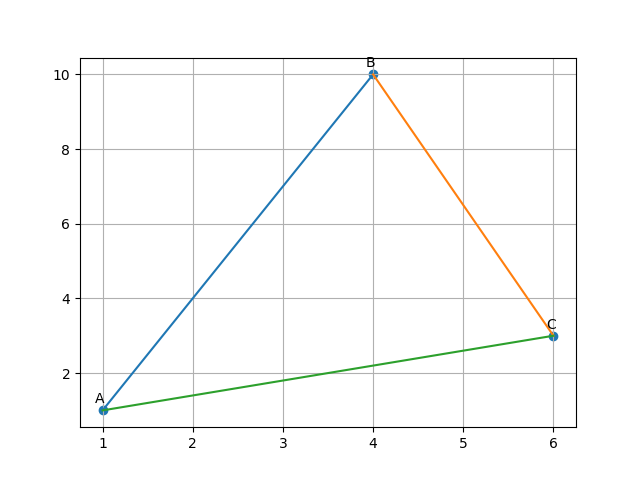
\includegraphics[width = \columnwidth]{./chapters/12/10/2/18/figs/triangle.png}
\caption{}
	\label{fig:chapters/12/10/2/18/}
\end{figure}
\solution
		\iffalse
\documentclass[journal,12pt,twocolumn]{IEEEtran}
\usepackage{romannum}
\usepackage{float}
\usepackage{setspace}
\usepackage{gensymb}
\singlespacing
\usepackage[cmex10]{amsmath}
\usepackage{amsthm}
\usepackage{mathrsfs}
\usepackage{txfonts}
\usepackage{stfloats}
\usepackage{bm}
\usepackage{cite}
\usepackage{cases}
\usepackage{subfig}
\usepackage{longtable}
\usepackage{multirow}
\usepackage{enumitem}
\usepackage{mathtools}
\usepackage{steinmetz}
\usepackage{tikz}
\usepackage{circuitikz}
\usepackage{verbatim}
\usepackage{tfrupee}
\usepackage[breaklinks=true]{hyperref}
\usepackage{tkz-euclide}
\usetikzlibrary{calc,math}
\usepackage{listings}
    \usepackage{color}                                            %%
    \usepackage{array}                                            %%
    \usepackage{longtable}                                        %%
    \usepackage{calc}                                             %%
    \usepackage{multirow}                                         %%
    \usepackage{hhline}                                           %%
    \usepackage{ifthen}                                           %%
  %optionally (for landscape tables embedded in another document): %%
    \usepackage{lscape}     
\usepackage{multicol}
\usepackage{chngcntr}
\DeclareMathOperator*{\Res}{Res}
\renewcommand\thesection{\arabic{section}}
\renewcommand\thesubsection{\thesection.\arabic{subsection}}
\renewcommand\thesubsubsection{\thesubsection.\arabic{subsubsection}}

\renewcommand\thesectiondis{\arabic{section}}
\renewcommand\thesubsectiondis{\thesectiondis.\arabic{subsection}}
\renewcommand\thesubsubsectiondis{\thesubsectiondis.\arabic{subsubsection}}

% correct bad hyphenation here
\hyphenation{op-tical net-works semi-conduc-tor}
\def\inputGnumericTable{}                                 %%

\lstset{
frame=single, 
breaklines=true,
columns=fullflexible
}

\begin{document}


\newtheorem{theorem}{Theorem}[section]
\newtheorem{problem}{Problem}
\newtheorem{proposition}{Proposition}[section]
\newtheorem{lemma}{Lemma}[section]
\newtheorem{corollary}[theorem]{Corollary}
\newtheorem{example}{Example}[section]
\newtheorem{definition}[problem]{Definition}
\newcommand{\BEQA}{\begin{eqnarray}}
\newcommand{\EEQA}{\end{eqnarray}}
\newcommand{\define}{\stackrel{\triangle}{=}}

\bibliographystyle{IEEEtran}
\providecommand{\mbf}{\mathbf}
\providecommand{\pr}[1]{\ensuremath{\Pr\left(#1\right)}}
\providecommand{\qfunc}[1]{\ensuremath{Q\left(#1\right)}}
\providecommand{\sbrak}[1]{\ensuremath{{}\left[#1\right]}}
\providecommand{\lsbrak}[1]{\ensuremath{{}\left[#1\right.}}
\providecommand{\rsbrak}[1]{\ensuremath{{}\left.#1\right]}}
\providecommand{\brak}[1]{\ensuremath{\left(#1\right)}}
\providecommand{\lbrak}[1]{\ensuremath{\left(#1\right.}}
\providecommand{\rbrak}[1]{\ensuremath{\left.#1\right)}}
\providecommand{\cbrak}[1]{\ensuremath{\left\{#1\right\}}}
\providecommand{\lcbrak}[1]{\ensuremath{\left\{#1\right.}}
\providecommand{\rcbrak}[1]{\ensuremath{\left.#1\right\}}}
\theoremstyle{remark}
\newtheorem{rem}{Remark}
\newcommand{\sgn}{\mathop{\mathrm{sgn}}}
\providecommand{\abs}[1]{\left\vert#1\right\vert}
\providecommand{\res}[1]{\Res\displaylimits_{#1}} 
\providecommand{\norm}[1]{\left\lVert#1\right\rVert}
\providecommand{\mtx}[1]{\mathbf{#1}}
\providecommand{\mean}[1]{E\left[ #1 \right]}
\providecommand{\fourier}{\overset{\mathcal{F}}{ \rightleftharpoons}}
\providecommand{\system}{\overset{\mathcal{H}}{ \longleftrightarrow}}
\newcommand{\solution}{\noindent \textbf{Solution: }}
\newcommand{\cosec}{\,\text{cosec}\,}
\providecommand{\dec}[2]{\ensuremath{\overset{#1}{\underset{#2}{\gtrless}}}}
\newcommand{\myvec}[1]{\ensuremath{\begin{pmatrix}#1\end{pmatrix}}}
\newcommand{\mydet}[1]{\ensuremath{\begin{vmatrix}#1\end{vmatrix}}}
\numberwithin{equation}{subsection}
\makeatletter
\@addtoreset{figure}{problem}
\makeatother

\let\StandardTheFigure\thefigure
\let\vec\mathbf
\renewcommand{\thefigure}{\theproblem}



\def\putbox#1#2#3{\makebox[0in][l]{\makebox[#1][l]{}\raisebox{\baselineskip}[0in][0in]{\raisebox{#2}[0in][0in]{#3}}}}
     \def\rightbox#1{\makebox[0in][r]{#1}}
     \def\centbox#1{\makebox[0in]{#1}}
     \def\topbox#1{\raisebox{-\baselineskip}[0in][0in]{#1}}
     \def\midbox#1{\raisebox{-0.5\baselineskip}[0in][0in]{#1}}

\vspace{3cm}


\title{Assignment 1}
\author{Jaswanth Chowdary Madala}





% make the title area
\maketitle

\newpage

%\tableofcontents

\bigskip

\renewcommand{\thefigure}{\theenumi}
\renewcommand{\thetable}{\theenumi}

\begin{enumerate}
\item In the following figure for the triangle ABC, which of the following is not true:

(A) $\overrightarrow{AB}+\overrightarrow{BC}+\overrightarrow{CA} = \overrightarrow{0}$

(B) $\overrightarrow{AB}+\overrightarrow{BC}-\overrightarrow{AC} = \overrightarrow{0}$

(C) $\overrightarrow{AB}+\overrightarrow{BC}+\overrightarrow{AC} = \overrightarrow{0}$

(D) $\overrightarrow{AB}-\overrightarrow{CB}+\overrightarrow{CA} = \overrightarrow{0}$

\textbf{Solution:}
\fi
		We know that,
\begin{align}
\overrightarrow{AB} = \vec{B} - \vec{A}\\
\overrightarrow{BC} = \vec{C} - \vec{B}\\
\overrightarrow{CA} = \vec{A} - \vec{C}
\end{align}
By usinig this we verify each of the given option

\begin{enumerate}
\item 
\begin{align}
\overrightarrow{AB}+\overrightarrow{BC}+\overrightarrow{CA} &=
\vec{B}-\vec{A} + \vec{C} - \vec{B} + \vec{A} - \vec{C}\\
 &= 0
\end{align}
Option A is correct.

\item
\begin{align}
\overrightarrow{AB}+\overrightarrow{BC}-\overrightarrow{AC} &=
\vec{B}-\vec{A} + \vec{C} - \vec{B} - (\vec{C} - \vec{A})\\
 &= 0
\end{align}
Option B is correct.

\item 
\begin{align}
\overrightarrow{AB}+\overrightarrow{BC}+\overrightarrow{AC} &=
\vec{B}-\vec{A} + \vec{C} - \vec{B} + \vec{C} - \vec{A}\\
 &= 2(\vec{C}-\vec{A})
\end{align}
Option C is incorrect.

\item
\begin{align}
\overrightarrow{AB}-\overrightarrow{CB}+\overrightarrow{CA} &=
\vec{B}-\vec{A} - (\vec{B} - \vec{C}) + \vec{A} - \vec{C}\\
 &= 0
\end{align}
Option D is correct.
\end{enumerate}
Verification: Let us take an example to verify 
\begin{align}
\vec{A} = \myvec{1\\1}, 
\vec{B} = \myvec{3\\1},
\vec{C} = \myvec{6\\6} \\
\overrightarrow{AB} = \vec{B} - \vec{A} = \myvec{2\\0}, 
\overrightarrow{BC} = \vec{C} - \vec{B} = \myvec{3\\5},
\overrightarrow{CA} = \vec{A} - \vec{C} = \myvec{-5\\-5} 
\end{align}
Thus,
\begin{align}
\overrightarrow{AB}+\overrightarrow{BC}+\overrightarrow{CA} = \myvec{2+3+(-5) \\ 0+5+(-5)} = \myvec{0 \\0}
\end{align}
Similarly other options can be verified.


\item A girl walks 4 km towards west, then she walks 3 km in a direction 30$^{\circ}$ east of north and stops. Determine the girl's displacement from her initial point of departure.\\
	\solution
		See  
\figref{fig:chapters/12/10/5/3Fig1}.
Let the initial position
be
\begin{align}
	\vec{A}=\myvec{0\\0}
\end{align}
After going west, the position becomes
\begin{align}
			\vec{B}=\myvec{-4\\0}
\end{align}
If the final position be $\vec{C}$, from the given information,
\begin{align}
	 \vec{C}-\vec{B}=3\myvec{\cos{60\degree}\\\sin{60\degree}}
	 \implies 
	\vec{C}  
=\myvec{\frac{-5}{2}\\[2pt] \frac{3\sqrt{3}}{2}}
\end{align}
which is the desired displacement. 
\begin{figure}[H] 
 \begin{center} 
 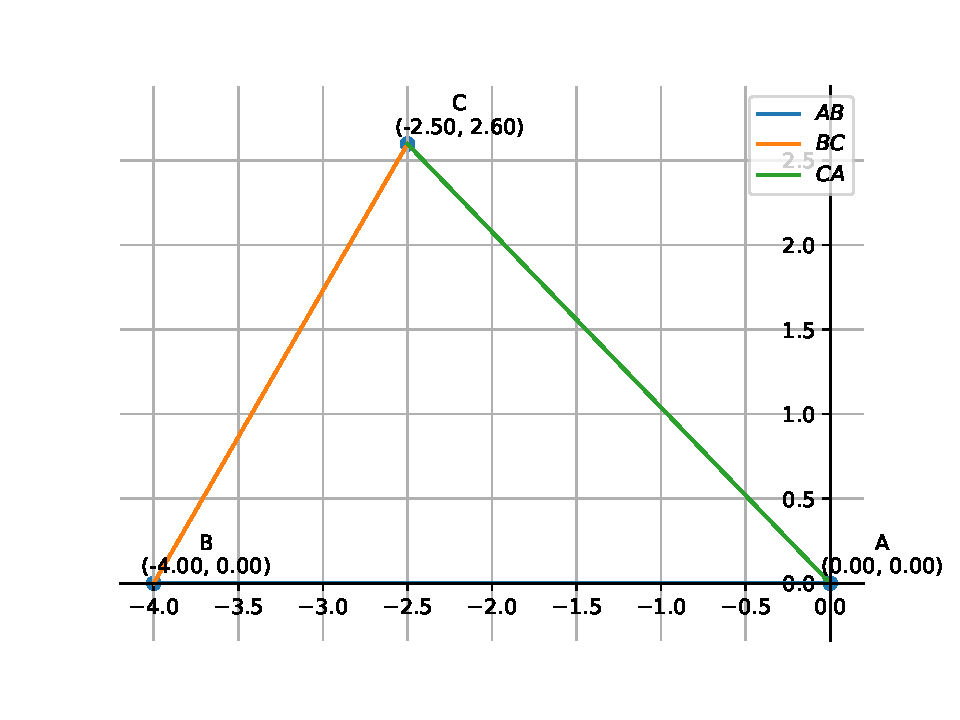
\includegraphics[width=0.75\columnwidth]{chapters/12/10/5/3/figs/fig.pdf} 
 \end{center} 
\caption{} 
\label{fig:chapters/12/10/5/3Fig1} 
\end{figure}

\item Without using distance formula, show that points A(– 2, – 1), B(4, 0), C(3, 3) and D(–3, 2) are the vertices of a parallelogram.
\label{chapters/11/10/1/9}
\\
\solution
	  From \eqref{eq:two-pgm},
\begin{align}
\vec{A}-\vec{B} = 
\vec{D}-\vec{C} =  \myvec{-6\\-1}
\end{align}
Hence, $ABCD$ is a parallelogram.
See \figref{fig:chapters/11/10/1/91}.
\begin{figure}[h!]
  \centering
   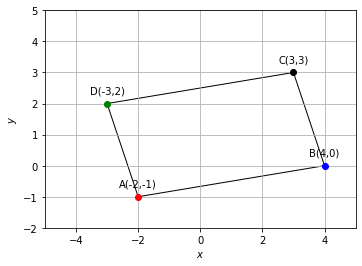
\includegraphics[width=\columnwidth]{chapters/11/10/1/9/figs/paralellogram.png}
    \caption{}
     \label{fig:chapters/11/10/1/91}  
\end{figure}




\item The fourth vertex $\vec{D}$ of a parallelogram $\vec{ABCD}$ whose three vertices are
	$\vec{A} (–2, 3), \vec{B} (6, 7)\text { and } \vec{C} (8, 3)$ is
\begin{enumerate}
	\item $(0, 1)$
	\item $(0, –1)$
	\item $ (–1,0)$
	\item$(1, 0)$
\end{enumerate}
\item Points $\vec{A}(4,3), \vec{B}(6,4),\vec{C}(5,-6)$  and  $\vec{D}(-3,5)$ are the vertices of a parallelogram.
\end{enumerate}

\newpage
\subsection{Section Formula}
\begin{enumerate}[label=\thesubsection.\arabic*,ref=\thesubsection.\theenumi]

\item Find the coordinates of the point which divides the join of $(-1,7) \text{ and } (4,-3)$ in the ratio 2:3.
	\\
		\solution
	Using section formula \eqref{eq:section_formula}, the desired point is
\begin{align}
\frac{1}{1+\frac{3}{2}}  \myvec{\myvec{
4\\
-3
}
  +
   \frac{3}{2}\myvec{
-1\\
7
}}
=\myvec{
1\\
3
}
\end{align}
See 
\figref{fig:chapters/10/7/2/1/Fig}
\begin{figure}[H]
\begin{center}
   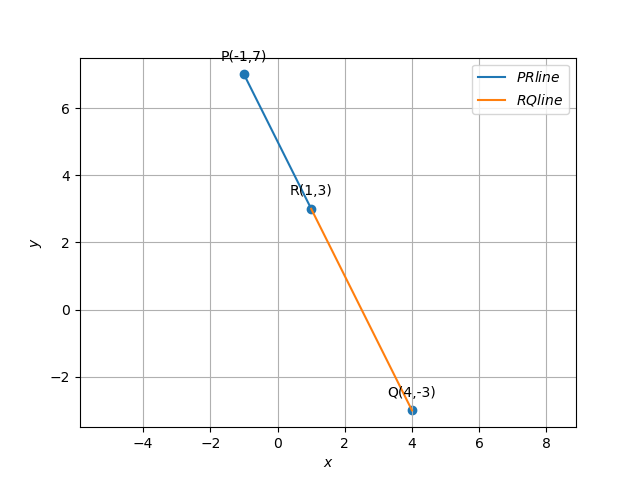
\includegraphics[width=0.75\columnwidth]{chapters/10/7/2/1/figs/linefig.png}
\end{center}
\caption{}
\label{fig:chapters/10/7/2/1/Fig}
\end{figure}


\item Find the coordinates of the points of trisection of the line segment joining $(4,-1)$  and  $(-2,3)$.
	\\
		\solution
	Using section formula,
\begin{align}
\vec{R}=\frac{1}{1+\frac{1}{2}}\brak{\myvec{4\\-1}+\frac{1}{2}\myvec{-2\\-3}}
=\myvec{2\\ \frac{-5}{3}}\\
\vec{S}=\frac{1}{1+\frac{2}{1}}\brak{\myvec{4\\-1}+\frac{2}{1}\myvec{-2\\-3}}
=\myvec{0\\ \frac{-7}{3}}
\end{align}
which are the desired points of trisection.
\iffalse
See
		\figref{fig:chapters/10/7/2/2/Figure}
\begin{figure}[H]
\centering
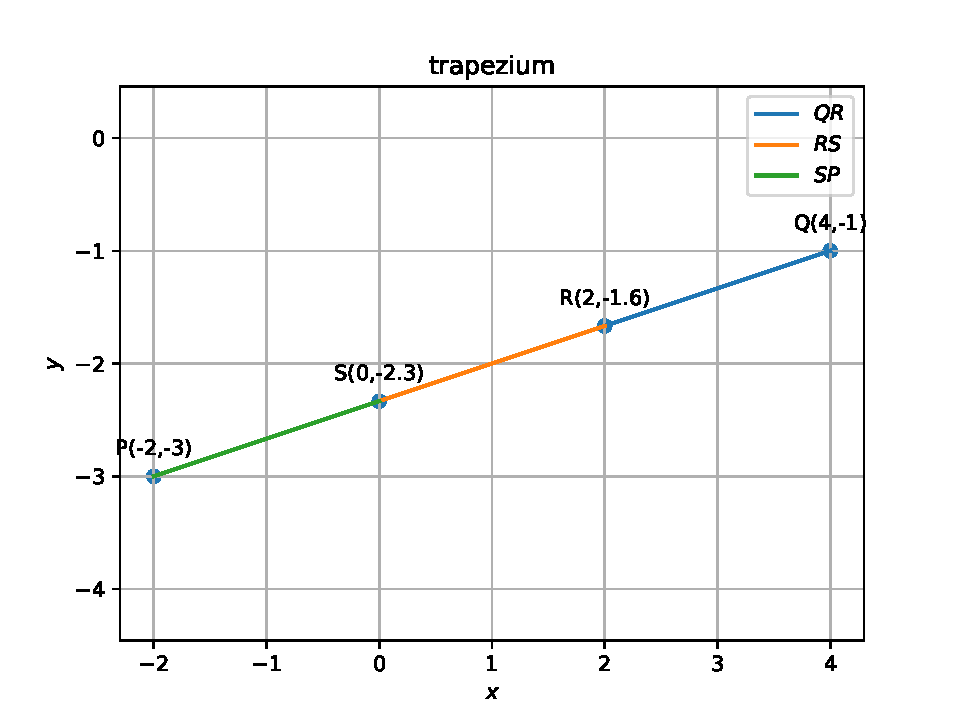
\includegraphics[width=0.75\columnwidth]{chapters/10/7/2/2/figs/dj.pdf}
\caption{}
		\label{fig:chapters/10/7/2/2/Figure}
\end{figure}
\fi

\item Find the ratio in which the line segment joining the points $(-3,10) \text{ and } (6,-8)$ $\text{ is divided by } (-1,6)$.
	\\
		\solution
	\iffalse
\documentclass[12pt]{article}
\usepackage{graphicx}
%\documentclass[journal,12pt,twocolumn]{IEEEtran}
\usepackage[none]{hyphenat}
\usepackage{graphicx}
\usepackage{listings}
\usepackage[english]{babel}
\usepackage{graphicx}
\usepackage{caption} 
\usepackage{hyperref}
\usepackage{booktabs}
\def\inputGnumericTable{}
\usepackage{color}                                            %%
    \usepackage{array}                                            %%
    \usepackage{longtable}                                        %%
    \usepackage{calc}                                             %%
    \usepackage{multirow}                                         %%
    \usepackage{hhline}                                           %%
    \usepackage{ifthen}
\usepackage{array}
\usepackage{amsmath}   % for having text in math mode
\usepackage{listings}
\lstset{
language=tex,
frame=single, 
breaklines=true
}
  
%Following 2 lines were added to remove the blank page at the beginning
\usepackage{atbegshi}% http://ctan.org/pkg/atbegshi
\AtBeginDocument{\AtBeginShipoutNext{\AtBeginShipoutDiscard}}
%
%New macro definitions
\newcommand{\mydet}[1]{\ensuremath{\begin{vmatrix}#1\end{vmatrix}}}
\providecommand{\brak}[1]{\ensuremath{\left(#1\right)}}
\providecommand{\norm}[1]{\left\lVert#1\right\rVert}
\newcommand{\solution}{\noindent \textbf{Solution: }}
\newcommand{\myvec}[1]{\ensuremath{\begin{pmatrix}#1\end{pmatrix}}}
\let\vec\mathbf
\begin{document}
\begin{center}
\title{\textbf{Coordinate Geometry}}
\date{\vspace{-5ex}} %Not to print date automatically
\maketitle
\end{center}
\setcounter{page}{1}
\section*{10$^{th}$ Maths - Chapter 7}
This is Problem-4 from Exercise 7.2
\begin{enumerate}
\item Find the ratio in which the line segement joining the points $\myvec{-3 \\ 10}$ and $\myvec{6\\-8}$ is divided by $\myvec{-1\\6}$.\\
\solution \\
\fi
		The input parameters for this problem are available in Table \eqref{tab:10/7/2/4-1}.
\begin{table}[ht!]
%%%%%%%%%%%%%%%%%%%%%%%%%%%%%%%%%%%%%%%%%%%%%%%%%%%%%%%%%%%%%%%%%%%%%%
%%                                                                  %%
%%  This is the header of a LaTeX2e file exported from Gnumeric.    %%
%%                                                                  %%
%%  This file can be compiled as it stands or included in another   %%
%%  LaTeX document. The table is based on the longtable package so  %%
%%  the longtable options (headers, footers...) can be set in the   %%
%%  preamble section below (see PRAMBLE).                           %%
%%                                                                  %%
%%  To include the file in another, the following two lines must be %%
%%  in the including file:                                          %%
%%        \def\inputGnumericTable{}                                 %%
%%  at the beginning of the file and:                               %%
%%        \input{name-of-this-file.tex}                             %%
%%  where the table is to be placed. Note also that the including   %%
%%  file must use the following packages for the table to be        %%
%%  rendered correctly:                                             %%
%%    \usepackage[latin1]{inputenc}                                 %%
%%    \usepackage{color}                                            %%
%%    \usepackage{array}                                            %%
%%    \usepackage{longtable}                                        %%
%%    \usepackage{calc}                                             %%
%%    \usepackage{multirow}                                         %%
%%    \usepackage{hhline}                                           %%
%%    \usepackage{ifthen}                                           %%
%%  optionally (for landscape tables embedded in another document): %%
%%    \usepackage{lscape}                                           %%
%%                                                                  %%
%%%%%%%%%%%%%%%%%%%%%%%%%%%%%%%%%%%%%%%%%%%%%%%%%%%%%%%%%%%%%%%%%%%%%%



%%  This section checks if we are begin input into another file or  %%
%%  the file will be compiled alone. First use a macro taken from   %%
%%  the TeXbook ex 7.7 (suggestion of Han-Wen Nienhuys).            %%
\def\ifundefined#1{\expandafter\ifx\csname#1\endcsname\relax}


%%  Check for the \def token for inputed files. If it is not        %%
%%  defined, the file will be processed as a standalone and the     %%
%%  preamble will be used.                                          %%
\ifundefined{inputGnumericTable}

%%  We must be able to close or not the document at the end.        %%
 \def\gnumericTableEnd{\end{document}}


%%%%%%%%%%%%%%%%%%%%%%%%%%%%%%%%%%%%%%%%%%%%%%%%%%%%%%%%%%%%%%%%%%%%%%
%%                                                                  %%
%%  This is the PREAMBLE. Change these values to get the right      %%
%%  paper size and other niceties.                                  %%
%%                                                                  %%
%%%%%%%%%%%%%%%%%%%%%%%%%%%%%%%%%%%%%%%%%%%%%%%%%%%%%%%%%%%%%%%%%%%%%%

 \documentclass[12pt%
     %,landscape%
                    ]{report}
       \usepackage[latin1]{inputenc}
       \usepackage{fullpage}
       \usepackage{color}
       \usepackage{array}
       \usepackage{longtable}
       \usepackage{calc}
       \usepackage{multirow}
       \usepackage{hhline}
       \usepackage{ifthen}

 \begin{document}


%%  End of the preamble for the standalone. The next section is for %%
%%  documents which are included into other LaTeX2e files.          %%
\else

%%  We are not a stand alone document. For a regular table, we will %%
%%  have no preamble and only define the closing to mean nothing.   %%
    \def\gnumericTableEnd{}

%%  If we want landscape mode in an embedded document, comment out  %%
%%  the line above and uncomment the two below. The table will      %%
%%  begin on a new page and run in landscape mode.                  %%
%       \def\gnumericTableEnd{\end{landscape}}
%       \begin{landscape}


%%  End f theoelse clause for this file being \input.              %%
\fi

%%%%%%%%%%%%%%%%%%%%%%%%%%%%%%%%%%%%%%%%%%%%%%%%%%%%%%%%%%%%%%%%%%%%%%
%%                                                                  %%
%%  The rest is the gnumeric table, except for the closing          %%
%%  statement. Changes below will alter the table's appearance.     %%
%%                                                                  %%
%%%%%%%%%%%%%%%%%%%%%%%%%%%%%%%%%%%%%%%%%%%%%%%%%%%%%%%%%%%%%%%%%%%%%%

\providecommand{\gnumericmathit}[1]{#1} 
%%  Uncomment the next line if you would like your numbers to be in %%
%%  italics if they are italizised in the gnumeric table.           %%
%\renewcommand{\gnumericmathit}[1]{\mathit{#1}}
\providecommand{\gnumericPB}[1]%
{\let\gnumericTemp=\\#1\let\\=\gnumericTemp\hspace{0pt}}
 \ifundefined{gnumericTableWidthDefined}
        \newlength{\gnumericTableWidth}
        \newlength{\gnumericTableWidthComplete}
        \newlength{\gnumericMultiRowLength}
        \global\def\gnumericTableWidthDefined{}
 \fi
%% The following setting protects this code from babel shorthands.  %%
 \ifthenelse{\isundefined{\languageshorthands}}{}{\languageshorthands{english}}
%%  The default table format retains the relative column widths of  %%
%%  gnumeric. They can easily be changed to c, r or l. In that case %%
%%  you may want to comment out the next line and uncomment the one %%
%%  thereafter                                                      %%
\providecommand\gnumbox{\makebox[0pt]}
%%\providecommand\gnumbox[1][]{\makebox}

%% to adjust positions in multirow situations                       %%
\setlength{\bigstrutjot}{\jot}
\setlength{\extrarowheight}{\doublerulesep}

%%  The \setlongtables command keeps column widths the same across  %%
%%  pages. Simply comment out next line for varying column widths.  %%
\setlongtables

\setlength\gnumericTableWidth{%
 53pt+%
 53pt+%
 82pt+%
 53pt+%
0pt}
\def\gumericNumCols{4}
\setlength\gnumericTableWidthComplete{\gnumericTableWidth+%
         \tabcolsep*\gumericNumCols*2+\arrayrulewidth*\gumericNumCols}
\ifthenelse{\lengthtest{\gnumericTableWidthComplete > \linewidth}}%
         {\def\gnumericScale{1*\ratio{\linewidth-%
                        \tabcolsep*\gumericNumCols*2-%
                        \arrayrulewidth*\gumericNumCols}%
{\gnumericTableWidth}}}%
{\def\gnumericScale{1}}

%%%%%%%%%%%%%%%%%%%%%%%%%%%%%%%%%%%%%%%%%%%%%%%%%%%%%%%%%%%%%%%%%%%%%%
%%                                                                  %%
%% The following are the widths of the various columns. We are      %%
%% defining them here because then they are easier to change.       %%
%% Depending on the cell formats we may use them more than once.    %%
%%                                                                  %%
%%%%%%%%%%%%%%%%%%%%%%%%%%%%%%%%%%%%%%%%%%%%%%%%%%%%%%%%%%%%%%%%%%%%%%

\ifthenelse{\isundefined{\gnumericColA}}{\newlength{\gnumericColA}}{}\settowidth{\gnumericColA}{\begin{tabular}{@{}p{53pt*\gnumericScale}@{}}x\end{tabular}}
\ifthenelse{\isundefined{\gnumericColB}}{\newlength{\gnumericColB}}{}\settowidth{\gnumericColB}{\begin{tabular}{@{}p{53pt*\gnumericScale}@{}}x\end{tabular}}
\ifthenelse{\isundefined{\gnumericColC}}{\newlength{\gnumericColC}}{}\settowidth{\gnumericColC}{\begin{tabular}{@{}p{82pt*\gnumericScale}@{}}x\end{tabular}}
\ifthenelse{\isundefined{\gnumericColD}}{\newlength{\gnumericColD}}{}\settowidth{\gnumericColD}{\begin{tabular}{@{}p{53pt*\gnumericScale}@{}}x\end{tabular}}

\begin{center}
\begin{tabular}[c]{%
 b{\gnumericColA}%
 b{\gnumericColB}%
 b{\gnumericColC}%
 b{\gnumericColD}%
 }

%%%%%%%%%%%%%%%%%%%%%%%%%%%%%%%%%%%%%%%%%%%%%%%%%%%%%%%%%%%%%%%%%%%%%%
%%  The longtable options. (Caption, headers... see Goosens, p.124) %%
% \caption{The Table Caption.}             \\ %
% \hline % Across the top of the table.
%%  The rest of these options are table rows which are placed on    %%
%%  the first, last or every page. Use \multicolumn if you want.    %%

%%  Header for the first page.                                      %%
% \multicolumn{4}{c}{The First Header} \\ \hline 
% \multicolumn{1}{c}{colTag} %Column 1
% &\multicolumn{1}{c}{colTag} %Column 2
% &\multicolumn{1}{c}{colTag} %Column 3
% &\multicolumn{1}{c}{colTag} \\ \hline %Last column
% \endfirsthead

%%  The running header definition.                                  %%
% \hline
% \multicolumn{4}{l}{\ldots\small\slshape continued} \\ \hline
% \multicolumn{1}{c}{colTag} %Column 1
% &\multicolumn{1}{c}{colTag} %Column 2
% &\multicolumn{1}{c}{colTag} %Column 3
% &\multicolumn{1}{c}{colTag} \\ \hline %Last column
% \endhead

%%  The running footer definition.                                  %%
% \hline
% \multicolumn{4}{r}{\small\slshape continued\ldots} \\
% \endfoot

%%  The ending footer definition.                                   %%
% \multicolumn{4}{c}{That's all folks} \\ \hline 
% \endlastfoot
%%%%%%%%%%%%%%%%%%%%%%%%%%%%%%%%%%%%%%%%%%%%%%%%%%%%%%%%%%%%%%%%%%%%%%

\hhline{|-|-|-~}
  \multicolumn{1}{|p{\gnumericColA}|}%
 {\gnumericPB{\centering}\gnumbox{\textbf{Symbol}}}
 &\multicolumn{1}{p{\gnumericColB}|}%
 {\gnumericPB{\centering}\gnumbox{\textbf{Value}}}
 &\multicolumn{1}{p{\gnumericColC}|}%
 {\gnumericPB{\centering}\gnumbox{\textbf{Description}}}
 &
\\
\hhline{|---|~}
  \multicolumn{1}{|p{\gnumericColA}|}%
 {\gnumericPB{\centering}\gnumbox{$\vec{P}$}}
 &\multicolumn{1}{p{\gnumericColB}|}%
 {\gnumericPB{\centering}\gnumbox{$\myvec{-3\\10}$}}
 &\multicolumn{1}{p{\gnumericColC}|}%
 {\gnumericPB{\centering}\gnumbox{First point}}
 &
\\
\hhline{|---|~}
  \multicolumn{1}{|p{\gnumericColA}|}%
 {\gnumericPB{\centering}\gnumbox{$\vec{Q}$}}
 &\multicolumn{1}{p{\gnumericColB}|}%
 {\gnumericPB{\centering}\gnumbox{$\myvec{6\\-8}$}}
 &\multicolumn{1}{p{\gnumericColC}|}%
 {\gnumericPB{\centering}\gnumbox{Second point}}
 &
\\
\hhline{|---|~}
  \multicolumn{1}{|p{\gnumericColA}|}%
 {\gnumericPB{\centering}\gnumbox{$\vec{R}$}}
 &\multicolumn{1}{p{\gnumericColB}|}%
 {\gnumericPB{\centering}\gnumbox{$\myvec{-1\\6}$}}
 &\multicolumn{1}{p{\gnumericColC}|}%
 {\gnumericPB{\centering}\gnumbox{Desired point}}
 &
\\
\hhline{|-|-|-|~}
\end{tabular}
 \end{center}

\ifthenelse{\isundefined{\languageshorthands}}{}{\languageshorthands{\languagename}}
\gnumericTableEnd

\caption{}
\label{tab:10/7/2/4-1} 
\end{table}
Using section formula,
\begin{align}
         \vec{R} &=\frac{\vec{Q}+n\vec{P}}{1+n}\label{eq:chapters/10/7/2/4/1}
\end{align}
Substituting the values of $\vec{P},\vec{Q}$ and $\vec{R}$ in \eqref{eq:chapters/10/7/2/4/1}
\begin{align}
         \myvec{-1\\6} &=\frac{{\myvec{-3\\10}+n\myvec{6\\-8}}}{1+n}\\
 &=\frac{1}{1+n}\brak{{\myvec{-3\\10}+n\myvec{6\\-8}}} \\
 &=\frac{1}{1+n}\myvec{-3+6n\\10-8n} \label{eq:chapters/10/7/2/4/4}
\end{align}
Simplifying \eqref{eq:chapters/10/7/2/4/4} yeilds,
\begin{align}
          -1 &=\frac{-3+6n}{1+n}\\
\implies          n &=\frac{2}{7}
\end{align}
Also,
\begin{align}
          6 &=\frac{10-8n}{1+n}\\
    \implies      n &=\frac{2}{7}
\end{align}
Hence the desired ratio is $\dfrac{2}{7}$.  
\begin{figure}[!h]
 \begin{center}
  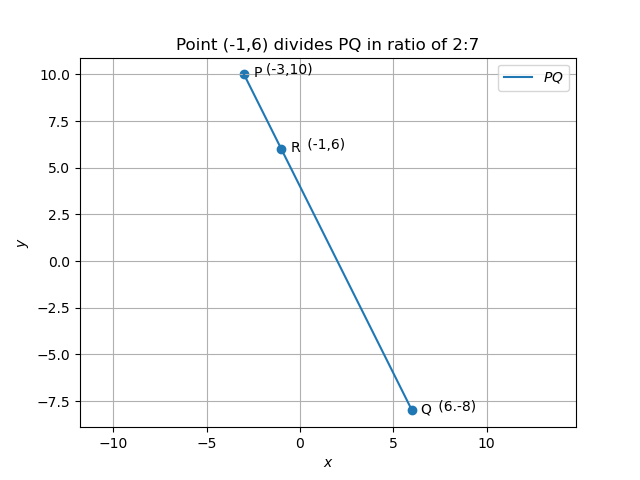
\includegraphics[width=\columnwidth]{chapters/10/7/2/4/figs/fig.png}
 \end{center}
\caption{}
\label{fig:10/7/2/4Fig1}
\end{figure}

\item If $(1,2), (4,y), (x,6), (3,5)$ are the vertices of a parallelogram taken in order, find x and y.
	\\
		\solution
	\iffalse
\documentclass[12pt]{article}
\usepackage{graphicx}
%\documentclass[journal,12pt,twocolumn]{IEEEtran}
\def\inputGnumericTable{}
\usepackage{color}                                            %%
    \usepackage{array}                                            %%
    \usepackage{longtable}                                        %%
    \usepackage{calc}                                             %%
    \usepackage{multirow}                                         %%
    \usepackage{hhline}                                           %%
    \usepackage{ifthen}
\usepackage[none]{hyphenat}
\usepackage{graphicx}
\usepackage{listings}
\usepackage[english]{babel}
\usepackage{graphicx}
\usepackage{caption} 
\usepackage{hyperref}
\usepackage{booktabs}
\usepackage{array}
\usepackage{amsmath}   % for having text in math mode
\usepackage{listings}
\lstset{
  frame=single,
  breaklines=true
}
  
%Following 2 lines were added to remove the blank page at the beginning
\usepackage{atbegshi}% http://ctan.org/pkg/atbegshi
\AtBeginDocument{\AtBeginShipoutNext{\AtBeginShipoutDiscard}}
%


%New macro definitions
\newcommand{\mydet}[1]{\ensuremath{\begin{vmatrix}#1\end{vmatrix}}}
\providecommand{\brak}[1]{\ensuremath{\left(#1\right)}}
\providecommand{\norm}[1]{\left\lVert#1\right\rVert}
\newcommand{\solution}{\noindent \textbf{Solution: }}
\newcommand{\myvec}[1]{\ensuremath{\begin{pmatrix}#1\end{pmatrix}}}
\let\vec\mathbf

\begin{document}

\begin{center}
\title{\textbf{Properties of Parallelegram}}
\date{\vspace{-5ex}} %Not to print date automatically
\maketitle
\end{center}

\setcounter{page}{1}

\section{10$^{th}$ Maths - Chapter 7}

This is Problem-6 from Exercise 7.2

\begin{enumerate}
\item If $\vec{A}(1, 2),\vec{B}(4, x),\vec{C}(y, 6) \text{and } \vec{D}(3, 5)$ are the vertices of a parallelogram taken in order,find x and y.
\end{enumerate}
\fi

The input parameters for this problem are available in
\ref{table:chapters/10/7/2/6/tables/}.	
\begin{table}[!ht]
	\centering
	%%%%%%%%%%%%%%%%%%%%%%%%%%%%%%%%%%%%%%%%%%%%%%%%%%%%%%%%%%%%%%%%%%%%%%
%%                                                                  %%
%%  This is the header of a LaTeX2e file exported from Gnumeric.    %%
%%                                                                  %%
%%  This file can be compiled as it stands or included in another   %%
%%  LaTeX document. The table is based on the longtable package so  %%
%%  the longtable options (headers, footers...) can be set in the   %%
%%  preamble section below (see PRAMBLE).                           %%
%%                                                                  %%
%%  To include the file in another, the following two lines must be %%
%%  in the including file:                                          %%
%%        \def\inputGnumericTable{}                                 %%
%%  at the beginning of the file and:                               %%
%%        \input{name-of-this-file.tex}                             %%
%%  where the table is to be placed. Note also that the including   %%
%%  file must use the following packages for the table to be        %%
%%  rendered correctly:                                             %%
%%    \usepackage[latin1]{inputenc}                                 %%
%%    \usepackage{color}                                            %%
%%    \usepackage{array}                                            %%
%%    \usepackage{longtable}                                        %%
%%    \usepackage{calc}                                             %%
%%    \usepackage{multirow}                                         %%
%%    \usepackage{hhline}                                           %%
%%    \usepackage{ifthen}                                           %%
%%  optionally (for landscape tables embedded in another document): %%
%%    \usepackage{lscape}                                           %%
%%                                                                  %%
%%%%%%%%%%%%%%%%%%%%%%%%%%%%%%%%%%%%%%%%%%%%%%%%%%%%%%%%%%%%%%%%%%%%%%



%%  This section checks if we are begin input into another file or  %%
%%  the file will be compiled alone. First use a macro taken from   %%
%%  the TeXbook ex 7.7 (suggestion of Han-Wen Nienhuys).            %%
\def\ifundefined#1{\expandafter\ifx\csname#1\endcsname\relax}


%%  Check for the \def token for inputed files. If it is not        %%
%%  defined, the file will be processed as a standalone and the     %%
%%  preamble will be used.                                          %%
\ifundefined{inputGnumericTable}

%%  We must be able to close or not the document at the end.        %%
	\def\gnumericTableEnd{\end{document}}


%%%%%%%%%%%%%%%%%%%%%%%%%%%%%%%%%%%%%%%%%%%%%%%%%%%%%%%%%%%%%%%%%%%%%%
%%                                                                  %%
%%  This is the PREAMBLE. Change these values to get the right      %%
%%  paper size and other niceties.                                  %%
%%                                                                  %%
%%%%%%%%%%%%%%%%%%%%%%%%%%%%%%%%%%%%%%%%%%%%%%%%%%%%%%%%%%%%%%%%%%%%%%

	\documentclass[12pt%
			  %,landscape%
                    ]{report}
       \usepackage[latin1]{inputenc}
       \usepackage{fullpage}
       \usepackage{color}
       \usepackage{array}
       \usepackage{longtable}
       \usepackage{calc}
       \usepackage{multirow}
       \usepackage{hhline}
       \usepackage{ifthen}

	\begin{document}


%%  End of the preamble for the standalone. The next section is for %%
%%  documents which are included into other LaTeX2e files.          %%
\else

%%  We are not a stand alone document. For a regular table, we will %%
%%  have no preamble and only define the closing to mean nothing.   %%
    \def\gnumericTableEnd{}

%%  If we want landscape mode in an embedded document, comment out  %%
%%  the line above and uncomment the two below. The table will      %%
%%  begin on a new page and run in landscape mode.                  %%
%       \def\gnumericTableEnd{\end{landscape}}
%       \begin{landscape}


%%  End of the else clause for this file being \input.              %%
\fi

%%%%%%%%%%%%%%%%%%%%%%%%%%%%%%%%%%%%%%%%%%%%%%%%%%%%%%%%%%%%%%%%%%%%%%
%%                                                                  %%
%%  The rest is the gnumeric table, except for the closing          %%
%%  statement. Changes below will alter the table's appearance.     %%
%%                                                                  %%
%%%%%%%%%%%%%%%%%%%%%%%%%%%%%%%%%%%%%%%%%%%%%%%%%%%%%%%%%%%%%%%%%%%%%%

\providecommand{\gnumericmathit}[1]{#1} 
%%  Uncomment the next line if you would like your numbers to be in %%
%%  italics if they are italizised in the gnumeric table.           %%
%\renewcommand{\gnumericmathit}[1]{\mathit{#1}}
\providecommand{\gnumericPB}[1]%
{\let\gnumericTemp=\\#1\let\\=\gnumericTemp\hspace{0pt}}
 \ifundefined{gnumericTableWidthDefined}
        \newlength{\gnumericTableWidth}
        \newlength{\gnumericTableWidthComplete}
        \newlength{\gnumericMultiRowLength}
        \global\def\gnumericTableWidthDefined{}
 \fi
%% The following setting protects this code from babel shorthands.  %%
 \ifthenelse{\isundefined{\languageshorthands}}{}{\languageshorthands{english}}
%%  The default table format retains the relative column widths of  %%
%%  gnumeric. They can easily be changed to c, r or l. In that case %%
%%  you may want to comment out the next line and uncomment the one %%
%%  thereafter                                                      %%
\providecommand\gnumbox{\makebox[0pt]}
%%\providecommand\gnumbox[1][]{\makebox}

%% to adjust positions in multirow situations                       %%
\setlength{\bigstrutjot}{\jot}
\setlength{\extrarowheight}{\doublerulesep}

%%  The \setlongtables command keeps column widths the same across  %%
%%  pages. Simply comment out next line for varying column widths.  %%
\setlongtables

\setlength\gnumericTableWidth{%
	53pt+%
	53pt+%
	82pt+%
	53pt+%
0pt}
\def\gumericNumCols{4}
\setlength\gnumericTableWidthComplete{\gnumericTableWidth+%
         \tabcolsep*\gumericNumCols*2+\arrayrulewidth*\gumericNumCols}
\ifthenelse{\lengthtest{\gnumericTableWidthComplete > \linewidth}}%
         {\def\gnumericScale{1*\ratio{\linewidth-%
                        \tabcolsep*\gumericNumCols*2-%
                        \arrayrulewidth*\gumericNumCols}%
{\gnumericTableWidth}}}%
{\def\gnumericScale{1}}

%%%%%%%%%%%%%%%%%%%%%%%%%%%%%%%%%%%%%%%%%%%%%%%%%%%%%%%%%%%%%%%%%%%%%%
%%                                                                  %%
%% The following are the widths of the various columns. We are      %%
%% defining them here because then they are easier to change.       %%
%% Depending on the cell formats we may use them more than once.    %%
%%                                                                  %%
%%%%%%%%%%%%%%%%%%%%%%%%%%%%%%%%%%%%%%%%%%%%%%%%%%%%%%%%%%%%%%%%%%%%%%

\ifthenelse{\isundefined{\gnumericColA}}{\newlength{\gnumericColA}}{}\settowidth{\gnumericColA}{\begin{tabular}{@{}p{53pt*\gnumericScale}@{}}x\end{tabular}}
\ifthenelse{\isundefined{\gnumericColB}}{\newlength{\gnumericColB}}{}\settowidth{\gnumericColB}{\begin{tabular}{@{}p{53pt*\gnumericScale}@{}}x\end{tabular}}
\ifthenelse{\isundefined{\gnumericColC}}{\newlength{\gnumericColC}}{}\settowidth{\gnumericColC}{\begin{tabular}{@{}p{82pt*\gnumericScale}@{}}x\end{tabular}}
\ifthenelse{\isundefined{\gnumericColD}}{\newlength{\gnumericColD}}{}\settowidth{\gnumericColD}{\begin{tabular}{@{}p{53pt*\gnumericScale}@{}}x\end{tabular}}

	\begin{center}
\begin{tabular}[c]{%
	b{\gnumericColA}%
	b{\gnumericColB}%
	b{\gnumericColC}%
	b{\gnumericColD}%
	}

%%%%%%%%%%%%%%%%%%%%%%%%%%%%%%%%%%%%%%%%%%%%%%%%%%%%%%%%%%%%%%%%%%%%%%
%%  The longtable options. (Caption, headers... see Goosens, p.124) %%
%	\caption{The Table Caption.}             \\	%
% \hline	% Across the top of the table.
%%  The rest of these options are table rows which are placed on    %%
%%  the first, last or every page. Use \multicolumn if you want.    %%

%%  Header for the first page.                                      %%
%	\multicolumn{4}{c}{The First Header} \\ \hline 
%	\multicolumn{1}{c}{colTag}	%Column 1
%	&\multicolumn{1}{c}{colTag}	%Column 2
%	&\multicolumn{1}{c}{colTag}	%Column 3
%	&\multicolumn{1}{c}{colTag}	\\ \hline %Last column
%	\endfirsthead

%%  The running header definition.                                  %%
%	\hline
%	\multicolumn{4}{l}{\ldots\small\slshape continued} \\ \hline
%	\multicolumn{1}{c}{colTag}	%Column 1
%	&\multicolumn{1}{c}{colTag}	%Column 2
%	&\multicolumn{1}{c}{colTag}	%Column 3
%	&\multicolumn{1}{c}{colTag}	\\ \hline %Last column
%	\endhead

%%  The running footer definition.                                  %%
%	\hline
%	\multicolumn{4}{r}{\small\slshape continued\ldots} \\
%	\endfoot

%%  The ending footer definition.                                   %%
%	\multicolumn{4}{c}{That's all folks} \\ \hline 
%	\endlastfoot
%%%%%%%%%%%%%%%%%%%%%%%%%%%%%%%%%%%%%%%%%%%%%%%%%%%%%%%%%%%%%%%%%%%%%%

\hhline{|-|-|-~}
	 \multicolumn{1}{|p{\gnumericColA}|}%
	{\gnumericPB{\centering}\gnumbox{\textbf{Symbol}}}
	&\multicolumn{1}{p{\gnumericColB}|}%
	{\gnumericPB{\centering}\gnumbox{\textbf{Value}}}
	&\multicolumn{1}{p{\gnumericColC}|}%
	{\gnumericPB{\centering}\gnumbox{\textbf{Description}}}
	&
\\
\hhline{|---|~}
	 \multicolumn{1}{|p{\gnumericColA}|}%
	{\gnumericPB{\centering}\gnumbox{$\vec{A}$}}
	&\multicolumn{1}{p{\gnumericColB}|}%
	{\gnumericPB{\centering}\gnumbox{$\myvec{1\\2}$}}
	&\multicolumn{1}{p{\gnumericColC}|}%
	{\gnumericPB{\centering}\gnumbox{First point}}
	&
\\
\hhline{|---|~}
	 \multicolumn{1}{|p{\gnumericColA}|}%
	{\gnumericPB{\centering}\gnumbox{$\vec{B}$}}
	&\multicolumn{1}{p{\gnumericColB}|}%
	{\gnumericPB{\centering}\gnumbox{$\myvec{4\\y}$}}
	&\multicolumn{1}{p{\gnumericColC}|}%
	{\gnumericPB{\centering}\gnumbox{Second point}}
	&
\\
\hhline{|---|~}
	 \multicolumn{1}{|p{\gnumericColA}|}%
	{\gnumericPB{\centering}\gnumbox{$\vec{C}$}}
	&\multicolumn{1}{p{\gnumericColB}|}%
	{\gnumericPB{\centering}\gnumbox{$\myvec{x\\6}$}}
	&\multicolumn{1}{p{\gnumericColC}|}%
	{\gnumericPB{\centering}\gnumbox{Third point}}
	&
\\
\hhline{|---|~}
	 \multicolumn{1}{|p{\gnumericColA}|}%
	{\gnumericPB{\centering}\gnumbox{$\vec{D}$}}
	&\multicolumn{1}{p{\gnumericColB}|}%
	{\gnumericPB{\centering}\gnumbox{$\myvec{3\\5}$}}
	&\multicolumn{1}{p{\gnumericColC}|}%
	{\gnumericPB{\centering}\gnumbox{Fourth point}}
	&
\\

\hhline{|-|-|-|~}
\end{tabular}
	\end{center}

\ifthenelse{\isundefined{\languageshorthands}}{}{\languageshorthands{\languagename}}
\gnumericTableEnd

\caption{}
\label{table:chapters/10/7/2/6/tables/}	
\end{table}
From the given information,
\begin{align}
  \label{eq:chapters/10/7/2/6/tables/det2f}
	\vec{B}-\vec{A} &= \myvec{4 \\y } - \myvec{1 \\2 }  = \myvec{3 \\y-2 }\\
	\vec{C}-\vec{D} &= \myvec{x \\6 } - \myvec{3 \\5 }  = \myvec{x-3 \\1}
\end{align}
Since $ABCD$ is a parallellogram,
\begin{align}
	\myvec{3\\y-2}&=\myvec{x-3\\1}\\
	\implies x&=6 ,y=3
\end{align}
Fig. \ref{fig:chapters/10/7/2/6/Fig3}
provides a verification.
\begin{figure}[h!]
	\begin{center}
  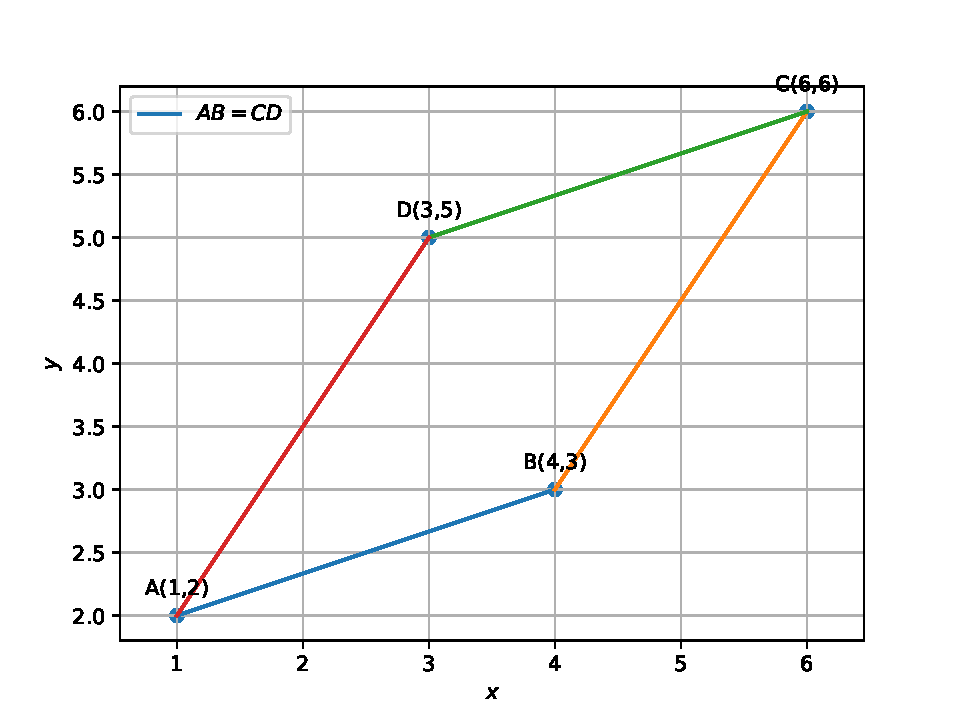
\includegraphics[width=\columnwidth]{chapters/10/7/2/6/figs/para.pdf}
	\end{center}
\caption{}
\label{fig:chapters/10/7/2/6/Fig3}
\end{figure}


\item Find the coordinates of a point A, where AB is the diameter of a circle whose centre is C$ (2,-3)$  and  B is $(1,4)$.
	\\
		\solution
		\begin{align}
	\vec{C} = \frac{\vec{A+B}}{2} 
	\implies 	\vec{A} = 2\vec{C}-\vec{B} 
	 = \myvec{3\\-10\\}	
	\end{align}       
	The radius is then obtained as
\begin{align}
	\norm{\vec{B}-\vec{C}} = 5\sqrt{2}
\end{align}
	See 
\figref{fig:chapters/10/7/2/7Fig}.
\begin{figure}[H]
\begin{center}	
	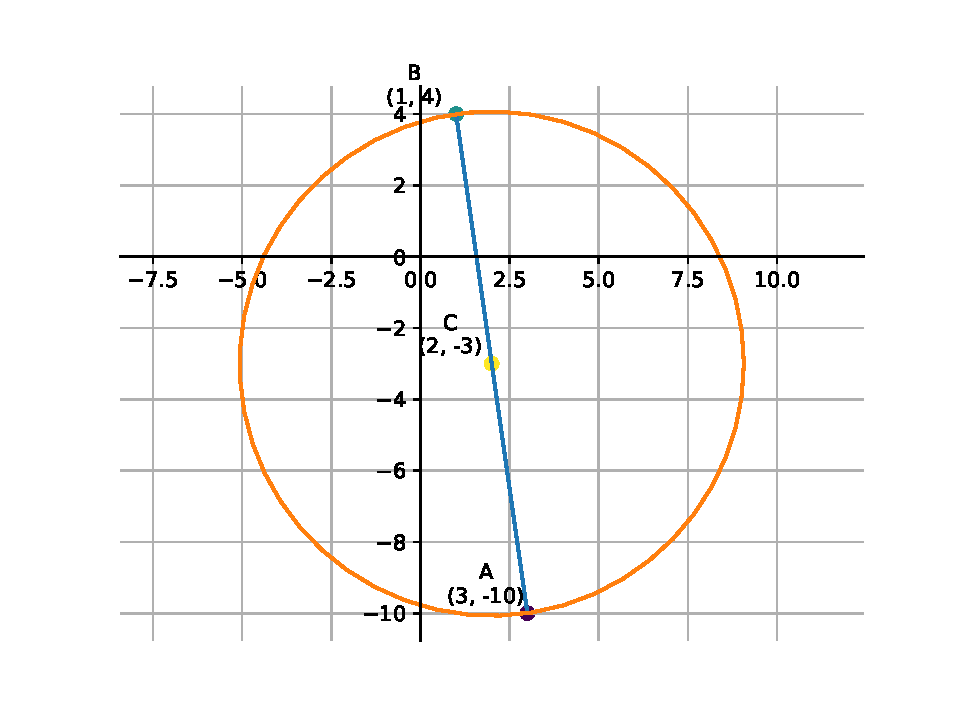
\includegraphics[width=0.75\columnwidth]{chapters/10/7/2/7/figs/fig.pdf}
\end{center}
\caption{}
\label{fig:chapters/10/7/2/7Fig}
\end{figure}
	

\item If A \text{ and } B are $(-2,-2) \text{ and } (2,-4)$, respectively, find the coordinates of P such that AP= $\frac {3}{7}$AB $\text{ and }$ P lies on the line segment AB.
	\\
		\solution
	Using section formula, 
\begin{align}
\vec{P}&=\frac{1}{1+\frac{3}{4}}\brak{\myvec{-2\\-2}+\frac{3}{4}\myvec{2\\-4}}
=\myvec{\frac{-2}{7}\\[1pt] \frac{-20}{7}}
\end{align}
\iffalse
See 
   \figref{fig:chapters/10/7/2/8/vec.png}.
\begin{figure}
   \centering 
 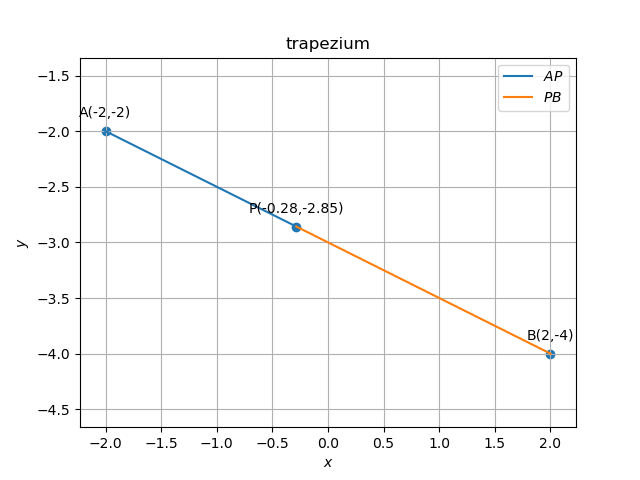
\includegraphics[width=0.75\columnwidth]{chapters/10/7/2/8/figs/vec.png}
   \caption{}
   \label{fig:chapters/10/7/2/8/vec.png}
   \end{figure}
   \fi

\item Find the coordinates of the points which divide the line segment joining $A(-2,2) \text{ and } B(2,8)$ into four equal parts.
	\\
		\solution
	Using section formula,
\begin{align}
	\vec{R}_k=\frac{\vec{B}+k\vec{A}}{1+k}, k = \frac{i}{n-i}, 0 < i < n
\end{align}
for $n = 4$.
See 
\figref{fig:chapters/10/7/2/9/Fig}.
\begin{figure}[H]
\begin{center}
   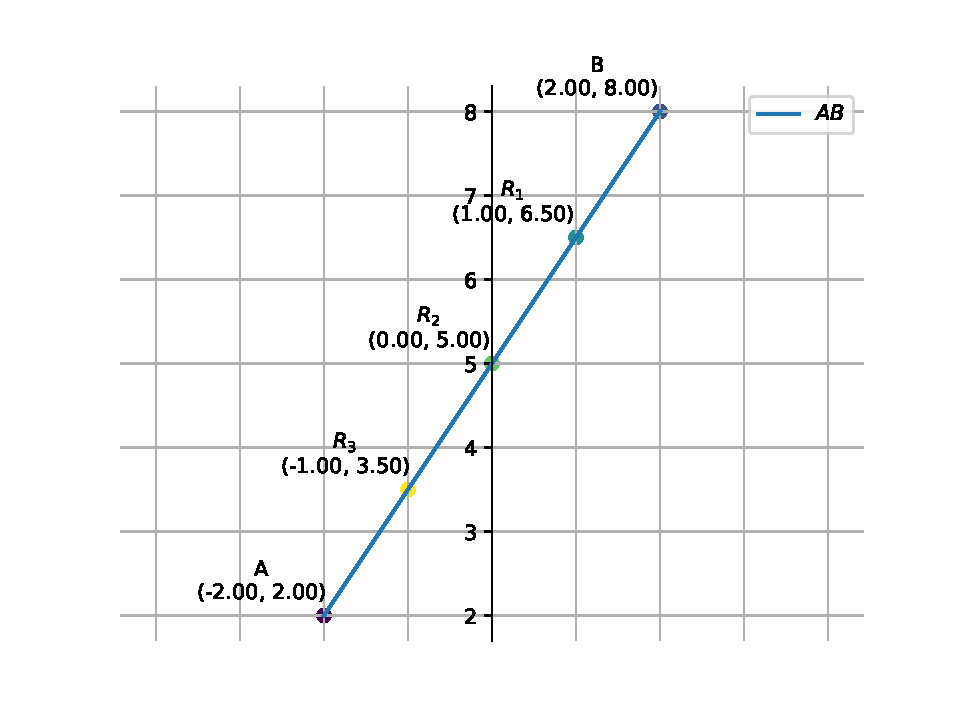
\includegraphics[width=0.75\columnwidth]{chapters/10/7/2/9/figs/fig.pdf}
\end{center}
\caption{}
\label{fig:chapters/10/7/2/9/Fig}
\end{figure}


\item Find the position vector of a point $\vec{R}$ which divides the line joining two points $\vec{P}$
and $\vec{Q}$ whose position vectors are $\hat{i}+2\hat{j}-\hat{k}$ and $-\hat{i}+\hat{j}+\hat{k}$ respectively, in the
ratio 2 : 1
\begin{enumerate}
    \item  internally
    \item  externally
\end{enumerate}
\solution
		\iffalse
\documentclass[journal,12pt,twocolumn]{IEEEtran}
%
\usepackage{setspace}
\usepackage{gensymb}
%\doublespacing
\singlespacing

%\usepackage{graphicx}
%\usepackage{amssymb}
%\usepackage{relsize}
\usepackage[cmex10]{amsmath}
%\usepackage{amsthm}
%\interdisplaylinepenalty=2500
%\savesymbol{iint}
%\usepackage{txfonts}
%\restoresymbol{TXF}{iint}
%\usepackage{wasysym}
\usepackage{amsthm}
%\usepackage{iithtlc}
\usepackage{mathrsfs}
\usepackage{txfonts}
\usepackage{stfloats}
\usepackage{bm}
\usepackage{cite}
\usepackage{cases}
\usepackage{subfig}
%\usepackage{xtab}
\usepackage{longtable}
\usepackage{multirow}
%\usepackage{algorithm}
%\usepackage{algpseudocode}
\usepackage{enumitem}
\usepackage{mathtools}
\usepackage{steinmetz}
\usepackage{tikz}
\usepackage{circuitikz}
\usepackage{verbatim}
\usepackage{tfrupee}
\usepackage[breaklinks=true]{hyperref}
%\usepackage{stmaryrd}
\usepackage{tkz-euclide} % loads  TikZ and tkz-base
%\usetkzobj{all}
\usetikzlibrary{calc,math}
\usepackage{listings}
    \usepackage{color}                                            %%
    \usepackage{array}                                            %%
    \usepackage{longtable}                                        %%
    \usepackage{calc}                                             %%
    \usepackage{multirow}                                         %%
    \usepackage{hhline}                                           %%
    \usepackage{ifthen}                                           %%
  %optionally (for landscape tables embedded in another document): %%
    \usepackage{lscape}     
\usepackage{multicol}
\usepackage{chngcntr}
%\usepackage{enumerate}
\usepackage{graphicx}

%\usepackage{wasysym}
%\newcounter{MYtempeqncnt}
\DeclareMathOperator*{\Res}{Res}
%\renewcommand{\baselinestretch}{2}
\renewcommand\thesection{\arabic{section}}
\renewcommand\thesubsection{\thesection.\arabic{subsection}}
\renewcommand\thesubsubsection{\thesubsection.\arabic{subsubsection}}

\renewcommand\thesectiondis{\arabic{section}}
\renewcommand\thesubsectiondis{\thesectiondis.\arabic{subsection}}
\renewcommand\thesubsubsectiondis{\thesubsectiondis.\arabic{subsubsection}}

% correct bad hyphenation here
\hyphenation{op-tical net-works semi-conduc-tor}
\def\inputGnumericTable{}                                 %%

\lstset{
%language=C,
frame=single, 
breaklines=true,
columns=fullflexible
}
%\lstset{
%language=tex,
%frame=single, 
%breaklines=true
%}

\begin{document}
%


\newtheorem{theorem}{Theorem}[section]
\newtheorem{problem}{Problem}
\newtheorem{proposition}{Proposition}[section]
\newtheorem{lemma}{Lemma}[section]
\newtheorem{corollary}[theorem]{Corollary}
\newtheorem{example}{Example}[section]
\newtheorem{definition}[problem]{Definition}
%\newtheorem{thm}{Theorem}[section] 
%\newtheorem{defn}[thm]{Definition}
%\newtheorem{algorithm}{Algorithm}[section]
%\newtheorem{cor}{Corollary}
\newcommand{\BEQA}{\begin{eqnarray}}
\newcommand{\EEQA}{\end{eqnarray}}
\newcommand{\define}{\stackrel{\triangle}{=}}

\bibliographystyle{IEEEtran}
%\bibliographystyle{ieeetr}


\providecommand{\mbf}{\mathbf}
\providecommand{\pr}[1]{\ensuremath{\Pr\left(#1\right)}}
\providecommand{\qfunc}[1]{\ensuremath{Q\left(#1\right)}}
\providecommand{\sbrak}[1]{\ensuremath{{}\left[#1\right]}}
\providecommand{\lsbrak}[1]{\ensuremath{{}\left[#1\right.}}
\providecommand{\rsbrak}[1]{\ensuremath{{}\left.#1\right]}}
\providecommand{\brak}[1]{\ensuremath{\left(#1\right)}}
\providecommand{\lbrak}[1]{\ensuremath{\left(#1\right.}}
\providecommand{\rbrak}[1]{\ensuremath{\left.#1\right)}}
\providecommand{\cbrak}[1]{\ensuremath{\left\{#1\right\}}}
\providecommand{\lcbrak}[1]{\ensuremath{\left\{#1\right.}}
\providecommand{\rcbrak}[1]{\ensuremath{\left.#1\right\}}}
\theoremstyle{remark}
\newtheorem{rem}{Remark}
\newcommand{\sgn}{\mathop{\mathrm{sgn}}}
\providecommand{\abs}[1]{\left\vert#1\right\vert}
\providecommand{\res}[1]{\Res\displaylimits_{#1}} 
\providecommand{\norm}[1]{\left\lVert#1\right\rVert}
%\providecommand{\norm}[1]{\lVert#1\rVert}
\providecommand{\mtx}[1]{\mathbf{#1}}
\providecommand{\mean}[1]{E\left[ #1 \right]}
\providecommand{\fourier}{\overset{\mathcal{F}}{ \rightleftharpoons}}
%\providecommand{\hilbert}{\overset{\mathcal{H}}{ \rightleftharpoons}}
\providecommand{\system}{\overset{\mathcal{H}}{ \longleftrightarrow}}
	%\newcommand{\solution}[2]{\textbf{Solution:}{#1}}
\newcommand{\solution}{\noindent \textbf{Solution: }}
\newcommand{\cosec}{\,\text{cosec}\,}
\providecommand{\dec}[2]{\ensuremath{\overset{#1}{\underset{#2}{\gtrless}}}}
\newcommand{\myvec}[1]{\ensuremath{\begin{pmatrix}#1\end{pmatrix}}}
\newcommand{\mydet}[1]{\ensuremath{\begin{vmatrix}#1\end{vmatrix}}}
%\numberwithin{equation}{section}
\numberwithin{equation}{subsection}
%\numberwithin{problem}{section}
%\numberwithin{definition}{section}
\makeatletter
\@addtoreset{figure}{problem}
\makeatother

\let\StandardTheFigure\thefigure
\let\vec\mathbf
%\renewcommand{\thefigure}{\theproblem.\arabic{figure}}
\renewcommand{\thefigure}{\theproblem}
%\setlist[enumerate,1]{before=\renewcommand\theequation{\theenumi.\arabic{equation}}
%\counterwithin{equation}{enumi}


%\renewcommand{\theequation}{\arabic{subsection}.\arabic{equation}}

\def\putbox#1#2#3{\makebox[0in][l]{\makebox[#1][l]{}\raisebox{\baselineskip}[0in][0in]{\raisebox{#2}[0in][0in]{#3}}}}
     \def\rightbox#1{\makebox[0in][r]{#1}}
     \def\centbox#1{\makebox[0in]{#1}}
     \def\topbox#1{\raisebox{-\baselineskip}[0in][0in]{#1}}
     \def\midbox#1{\raisebox{-0.5\baselineskip}[0in][0in]{#1}}

\vspace{3cm}

\title{EE2802: Assignment2}
\author{Nikam Pratik Balasaheb}





% make the title area
\maketitle

\newpage

%\tableofcontents

\bigskip

\renewcommand{\thefigure}{\theenumi}
\renewcommand{\thetable}{\theenumi}
%\renewcommand{\theequation}{\theenumi}

\section{Problem}
Find the position vector of a point R which divides the line joining two points P = $\myvec{1\\ 2 \\-1}$ and Q = $\myvec{ -1\\1\\1 }$ in the ratio 2:1 
\begin{enumerate}
\item internally
\item externally
\end{enumerate}

\section{Solution}

\begin{align}
\vec{P} = \myvec{ 1\\2\\-1} \\
 \vec{Q} = \myvec{ -1\\1\\1}
\end{align}

\fi

\begin{enumerate}


\item When $\vec{R}$ divides line segment joining $\vec{P}$ and $\vec{Q}$ internally,
\begin{align}
\vec{R} &= \frac{2 \vec{P} + 1 \vec{Q}}{3} \\
 &= \frac{2}{3} \vec{P} + \frac{1}{3} \vec{Q}\\
\vec{R} &= \myvec{\frac{1}{3}\\[1pt] \frac{5}{3} \\[1pt] \frac{-1}{3}}
\end{align}

\item When $\vec{R}$ divides line segment joining $\vec{P}$ and $\vec{Q}$ externally,
\begin{align}
\vec{R} &= 2 \vec{Q} - \vec{P} \\
 &= 2 \myvec{ -1\\1\\1} - \myvec{ 1\\2\\-1}\\
\vec{R} &= \myvec{ -3\\ 0 \\ 3 }
\end{align}


\end{enumerate}
See Fig. 
\ref{fig:chapters/12/10/2/15/}.
\begin{figure}[!ht]
\centering
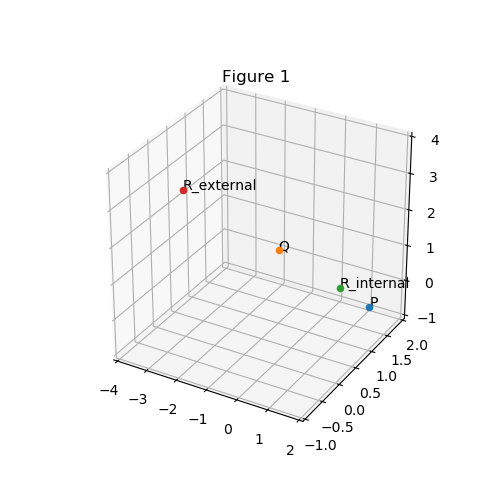
\includegraphics[width=\columnwidth]{chapters/12/10/2/15/figs/Figure_1.png}
\caption{}
\label{fig:chapters/12/10/2/15/}
\end{figure}



\item Find the position vector of the mid point of the vector joining the points $\vec{P}$(2, 3, 4)
and $\vec{Q}$(4, 1, –2).
\\
\solution
		The desired vector is
\begin{align}
\frac{1}{2}\myvec{2\\3\\4} +  \frac{1}{2}\myvec{4\\1\\-2} =\myvec{3\\2\\1} 
\end{align}




\item Determine the ratio in which the line $2x+y  - 4=0$ divides the line segment joining the points $\vec{A}(2, - 2)$  and  $\vec{B}(3, 7)$.
\\
\solution
	\iffalse
\documentclass[journal,12pt,twocolumn]{IEEEtran}
\usepackage{graphicx}
\graphicspath{{./chapters/10/7/4/1/figs/}}{}
\usepackage{amsmath,amssymb,amsfonts,amsthm}
\newcommand{\myvec}[1]{\ensuremath{\begin{pmatrix}#1\end{pmatrix}}}
\providecommand{\norm}[1]{\lVert#1\rVert}
\usepackage{listings}
\usepackage{watermark}
\usepackage{titlesec}
\usepackage{caption}
\let\vec\mathbf
\lstset{
frame=single, 
breaklines=true,
columns=fullflexible
}
\thiswatermark{\centering \put(0,-105.0){
\includegraphics[scale=0.15]{/sdcard/IITH/vector/vectpr-4/chapters/10/7/4/1/figs/logo.png}} }
\title{\mytitle}
\title{
Assignment - Vector-4
}
\author{Surajit Sarkar}
\begin{document}
\maketitle
%\tableofcontents
\bigskip
\section{\textbf{Problem}}
Determine the ratio in which the line 2x+y–4=0 divides the line segment joining the points A(2,–2) and B(3,7).
\section{\textbf{Solution}}
\begin{table}[h]
    \centering
    \begin{tabular}{|c|c|}
       \hline
       \textbf{Symbol}&\textbf{Value}  \\
       \hline
	    $\vec{A}$ & $\myvec{2\\-2}$\\
        \hline
	    $\vec{B}$ & $\myvec{3\\7}$\\
        \hline
	    c&$4$\\
        \hline
       $\vec{n}$ & $\myvec{2\\1}$\\
       \hline
    \end{tabular}
    \caption{Parameters}
    \label{tab:my_label}
\end{table}
Given equation
\fi
The given equation can be expressed as
\begin{align}
    \myvec{2&1}\vec{x}&=4\\
\end{align}
Using section formula, the point of division 
\begin{align}
    \vec{P} = \frac{k\vec{B+A}}{k+1}
\end{align}
which upon substitution in the equation of a line yields
\begin{align}
    \implies\vec{n}^{\top}\myvec{\frac{k\vec{B+A}}{k+1}}&=c\\
    \implies k&=\frac{c-\vec{n}^{\top}\vec{A}}{\vec{n}^{\top}\vec{B}-c}\\
\end{align}
upon simplification.  Substituting numerical values, 
\begin{align}
    k=\frac{2}{9}
\end{align}
See Fig. 
\ref{fig:chapters/10/7/4/1vec}.
\begin{figure}[!h]
\centering
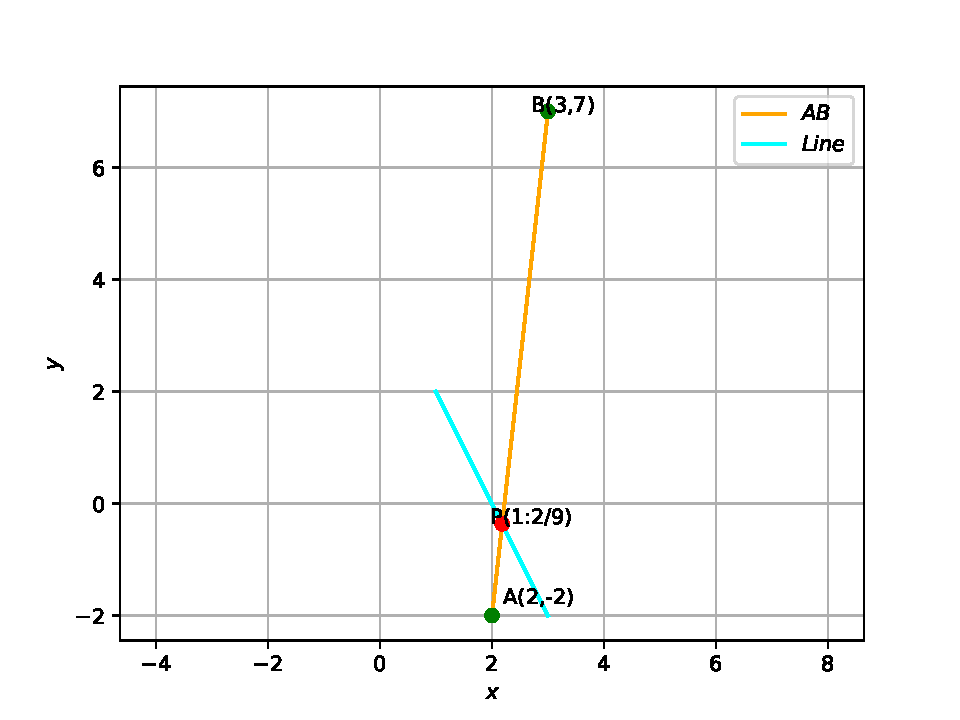
\includegraphics[width=\columnwidth]{chapters/10/7/4/1/figs/vec.pdf}
\caption{}
\label{fig:chapters/10/7/4/1vec}
\end{figure}


\item Let $\vec{A}(4, 2), \vec{B}(6, 5)$  and $ \vec{C}(1, 4)$ be the vertices of $\triangle ABC$.
\begin{enumerate}
\item The median from $\vec{A}$ meets $BC$ at $\vec{D}$. Find the coordinates of the point $\vec{D}$.
\item Find the coordinates of the point $\vec{P}$ on $AD$ such that $AP : PD = 2 : 1$.
\item Find the coordinates of points $\vec{Q}$ and $\vec{R}$ on medians $BE$ and $CF$ respectively such that $BQ : QE = 2 : 1$  and  $CR : RF = 2 : 1$.
\item What do you observe?
\item If $\vec{A}, \vec{B}$ and $\vec{C}$  are the vertices of $\triangle ABC$, find the coordinates of the centroid of the triangle.
\end{enumerate}
\solution
	\iffalse
\documentclass[12pt]{article}
\usepackage{graphicx}
\usepackage[none]{hyphenat}
\usepackage{graphicx}
\usepackage{listings}
\usepackage[english]{babel}
\usepackage{graphicx}
\usepackage{caption} 
\usepackage{booktabs}
\usepackage{array}
\usepackage{amssymb} % for \because
\usepackage{amsmath}   % for having text in math mode
\usepackage{extarrows} % for Row operations arrows
\usepackage{listings}
\usepackage[utf8]{inputenc}
\lstset{
  frame=single,
  breaklines=true
}
\usepackage{hyperref}
  
%Following 2 lines were added to remove the blank page at the beginning
\usepackage{atbegshi}% http://ctan.org/pkg/atbegshi
\AtBeginDocument{\AtBeginShipoutNext{\AtBeginShipoutDiscard}}


%New macro definitions
\newcommand{\mydet}[1]{\ensuremath{\begin{vmatrix}#1\end{vmatrix}}}
\providecommand{\brak}[1]{\ensuremath{\left(#1\right)}}
\newcommand{\solution}{\noindent \textbf{Solution: }}
\newcommand{\myvec}[1]{\ensuremath{\begin{pmatrix}#1\end{pmatrix}}}
\providecommand{\norm}[1]{\left\lVert#1\right\rVert}
\providecommand{\abs}[1]{\left\vert#1\right\vert}
\let\vec\mathbf

\begin{document}

\begin{center}
\title{\textbf{VECTORS}}
\date{\vspace{-5ex}} %Not to print date automatically
\maketitle
\end{center}

\section{10$^{th}$ Maths - EXERCISE-7.4}

Let A(4, 2), B(6, 5) and C(1, 4) be the vertices of $\triangle ABC$
\begin{enumerate}
\item The median from A meets BC at D. Find the coordinates of the point D.
\item Find the coordinates of the point P on AD such that $AP : PD = 2 : 1$
\item Find the coordinates of points Q and R on medians BE and CF respectively such
that $BQ : QE = 2 : 1 \text{and} CR : RF = 2 : 1.$
\item What do yo observe?
\item If $A(x_1, y_1), B(x_2, y_2) \text{and} C(x_3, y_3)$ are the vertices of $\triangle ABC$, find the coordinates of the centroid of the triangle.
\end{enumerate}

Given points are
\begin{align}
\vec{A}=\myvec{4\\ 2} ,
\vec{B}=\myvec{6\\ 5} ,
\vec{C}=\myvec{1\\ 4}
\end{align}
\fi

\begin{enumerate}
\item 
\begin{align}
\vec{D}&=\frac{\vec{B}+\vec{C}}{2}\\
&=\myvec{\frac{7}{2}\\[2pt] \frac{9}{2}}\\
\vec{E}&=\frac{\vec{A}+\vec{C}}{2}\\
&=\myvec{\frac{5}{2}\\ 3}\\
\vec{F}&=\frac{\vec{A}+\vec{B}}{2}\\
&=\myvec{5\\ \frac{7}{2}}
\end{align}

\item 
	For
$n=2$,
\begin{align}
\vec{P}&=\frac{1}{1+n}\brak{\myvec{\vec{A}+n\vec{D}}}\\
&=\frac{1}{3}\myvec{11\\11}
\end{align}

\item 
\begin{align}
\vec{Q}&=\frac{1}{1+n}\brak{\myvec{\vec{B}+n\vec{E}}}\\
&=\frac{1}{3}\myvec{11\\11}\\
\vec{R}&=\frac{1}{1+n}\brak{\myvec{\vec{C}+n\vec{F}}}\\
&=\frac{1}{3}\myvec{11\\11}\\
\end{align}

\item 
 $\vec{P},\vec{Q},\vec{R}$ are the same point.
   
\item 
\begin{align}
\vec{G}&=\frac{\vec{D}+\vec{E}+\vec{F}}{3}\\
&=\frac{1}{3}\myvec{11\\11}\\
\end{align} 
\end{enumerate}
See Fig.  
  \ref{fig:chapters/10/7/4/7/Figure}.
\begin{figure}[h!]
\centering
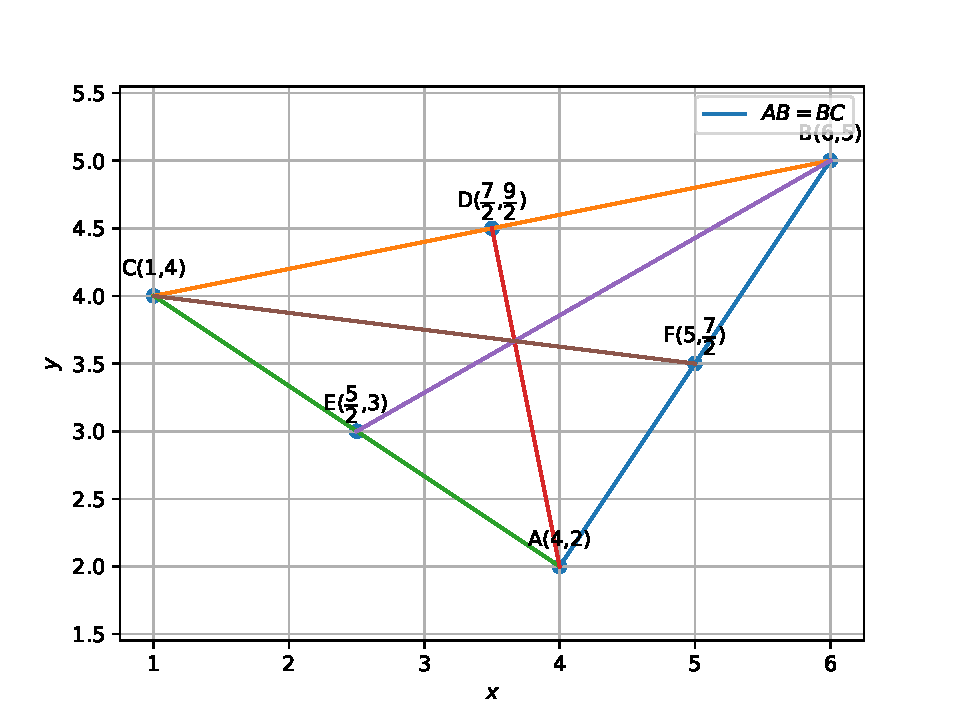
\includegraphics[width=\columnwidth]{chapters/10/7/4/7/figs/dj.pdf}
\caption{}
  \label{fig:chapters/10/7/4/7/Figure}
\end{figure}

\item Find the position vector of a point R which divides the line joining two points P and Q whose position vectors are $(2\vec{a}+\vec{b})$ and $(\vec{a}-3\vec{b})$
externally in the ratio 1 : 2. Also, show that P is the mid point of the line segment RQ.\\
	\solution
		\iffalse
\documentclass[10pt]{article}
\usepackage{graphicx}
\usepackage[none]{hyphenat}
\usepackage{graphicx}
\usepackage{listings}
\usepackage[english]{babel}
\usepackage{siunitx}
\usepackage{graphicx}
\usepackage{caption} 
\usepackage{booktabs}
\usepackage{array}
\usepackage{amssymb} % for \because
\usepackage{amsmath}   % for having text in math mode
\usepackage{extarrows} % for Row operations arrows
\usepackage{listings}
\usepackage[utf8]{inputenc}
\lstset{
  frame=single,
  breaklines=true
}
\usepackage{hyperref}
  
%Following 2 lines were added to remove the blank page at the beginning
\usepackage{atbegshi}% http://ctan.org/pkg/atbegshi
\AtBeginDocument{\AtBeginShipoutNext{\AtBeginShipoutDiscard}}


%New macro definitions
\newcommand{\mydet}[1]{\ensuremath{\begin{vmatrix}#1\end{vmatrix}}}
\providecommand{\brak}[1]{\ensuremath{\left(#1\right)}}
\newcommand{\solution}{\noindent \textbf{Solution: }}
\newcommand{\myvec}[1]{\ensuremath{\begin{pmatrix}#1\end{pmatrix}}}
\providecommand{\norm}[1]{\left\lVert#1\right\rVert}
\providecommand{\abs}[1]{\left\vert#1\right\vert}
\let\vec\mathbf{}
\begin{document}

\begin{center}
\title{\textbf{VECTORS}}
\date{\vspace{-5ex}} %Not to print date automatically
\maketitle
\end{center}

\section*{12$^{th}$ Maths - EXERCISE-10.5}

Find the position vector of a point R which divides the line joining two points  P and Q whose position vectors are P = $\myvec{2\\ 1 \\}$ and Q = $\myvec{ 1\\-3\\ }$  externally in the ratio 1:2.Also show that P is the midpoint of the linesegment RQ.

\solution

\begin{align}
\vec{P} = \myvec{ 2\\1\\} 
 \label{eq1} \\
 \vec{Q} = \myvec{ 1\\-3\\}
\end{align}
\fi
When $\vec{R}$ divides line segment joining $\vec{P}$ and $\vec{Q}$ externally,
\begin{align}
\vec{R} &= \frac{\vec{Q} -2\vec{P}}{-1} 
= \myvec{3\\5}
\end{align}
Also,
\begin{align}
\frac{ (\vec{R} + \vec{Q})}{2}
=\myvec{2\\1} =\vec{P}
\end{align}
See Fig. 
\ref{fig:chapters/12/10/5/9/Figure1}.
\begin{figure}[!h]
	\begin{center}
		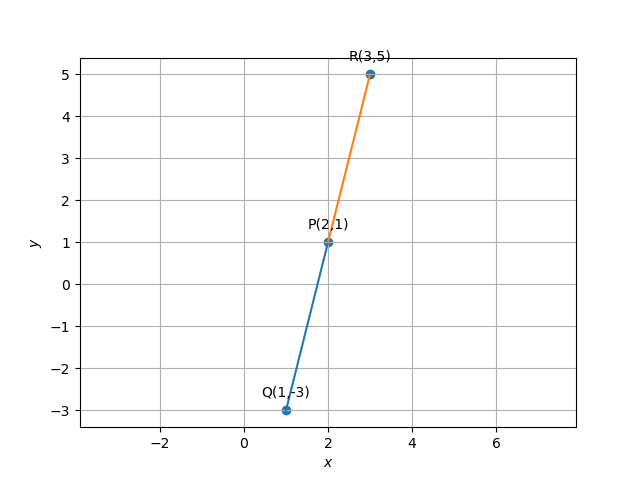
\includegraphics[width=\columnwidth]{chapters/12/10/5/9/figs/line.png}
	\end{center}
\caption{}
\label{fig:chapters/12/10/5/9/Figure1}
\end{figure}

\item The point which divides the line segment joining the points $\vec{P} (7, –6) $  and  $\vec{Q}(3, 4)$ in the 
ratio 1 : 2 internally lies in the
\begin{enumerate}
\item I quadrant
\item  II quadrant
\item  III quadrant
\item  IV quadrant
\end{enumerate}
\item If the point $\vec{P} (2, 1)$ lies on the line segment joining points$\vec{A} (4, 2)$  and $ \vec{B} (8, 4)$,
then
\begin{enumerate}
	\item $AP =\frac{1}{3}{AB}$ 
\item ${AP}={PE}$
\item ${PB}=\frac{1}{3}{AB}$
\item${AP}=\frac{1}{2}{AB}$
 \end{enumerate}
 \item If  $\vec{P}\frac{a}{3}$ is the mid-point of the line segment joining the points $\vec{Q} (– 6, 5)$  and $\vec{R}(– 2, 3),$ then the value of $a$ is
\begin{enumerate}
\item – 4
\item – 12
\item 12
\item – 6
\end{enumerate}
\item A line intersects the y-axis and x-axis of the points $\vec{P}$  and $\vec{Q}$, respectiveiy. lf $(2,5)$ is the mid-point of $\vec{PQ}$, then the coordinates of $\vec{P}$ and $ \vec{Q}$ are, respectively
\begin{enumerate}
	\item$(0,-5)$ and $(2,0)$
	\item$(0,-10)$ and $(-4,0)$
	\item$(0,4)$ and  $(-10,0)$
	\item$(0,-10)$ and $(4,0)$
\end{enumerate}
\item Point $\vec{P}(5,-3)$ is one of the two points of trisection of line segment joining the points $\vec{A}(7,-2)\text{ and }\vec{B}(1,-5)$
\item Points $\vec{A}(-6,10),\vec{B}(-4,6) \text{ and } \vec{C}(3,-8)$ are collinear such that $\vec{A}\vec{B}=  \frac{2}{9}\vec{A}\vec{C}$
\item In what ratio does the $x$-axis divide the line segment joining the points $(-4,-6)\text{ and }(-1,7)$? Find the coordinates of the point of division.
\item Find the ratio in which the point $\vec{P}\brak{\frac{3}{4},\frac{5}{12}}$ divides the line segment joining the points $\vec{A}\brak{\frac{1}{2},\frac{3}{2}}\text{ and } \vec{B}(2,-5)$.
\item If $\vec{P}(9a-2,-b)$ divides line segment joining $\vec{A}(3a+1,-3)\text{ and }\vec{B}(8a,5)$ in the ratio 3:1, find the values of $a$ and $b$.
\item The line segment joining the points $\vec{A}(3,2)\text{ and }\vec{B}(5,1)$ is divided at the point $\vec{P}$ in the ratio 1:2 which lies on $3x-18y+k=0$. Find the value of $k$.  
\item Find the coordinates of the point $\vec{R}$ on the line segment joining the points $\vec{P}(-1,3)\text{ and }\vec{Q}(2,5)$ such that $\vec{PR}={\frac{3}{5}}\vec{PQ}$.
\item Find the ratio in which the line 2x+3y-5=0 divides the line segment joining the points $(8,-9)\text{ and }(2,1)$. Also find the coordinates of the point of division,
\item If $\vec{a}$ $\text{and}$ $\vec{b}$ are the postion vectors of A and B, respectively, find the position vector of a point C in BA produced such that BC=1.5BA.
\item The position vector of the point which divides the join of points 2$\vec{a}$-3$\vec{b}$ $\text{and}$ $\vec{a}+\vec{b}$ in the ratio 3:1 is
	\begin{enumerate}
\item $\frac{3\vec{a}-2\vec{b}}{2}$
\item $\frac{7\vec{a}-8\vec{b}}{4}$
\item $\frac{\vec{3a}}{4}$
\item $\frac{\vec{5a}}{4}$
\end{enumerate}
\item Find the ratio in which the line segment joining $A(1,-5) \text{ and } B(-4,5)$ $\text{is divided by the x-axis}$. Also find the coordinates of the point of division.
\item Find the position vector of a point $\vec{R}$ which divides the line joining two points $\vec{P}$ and $\vec{Q}$ whose position vectors are $2\vec{a}+\vec{b}$ and $\vec{a}-3\vec{b}$ externally in the ratio $1:2$.
\end{enumerate}


\subsection{Rank}
\begin{enumerate}[label=\thesubsection.\arabic*,ref=\thesubsection.\theenumi]
\item Determine if the points $(1,5),(2,3)$ and $(-2,-11)$ are collinear.
	\\
		\iffalse
\documentclass[12pt]{article}
\usepackage{graphicx}
\usepackage[none]{hyphenat}
\usepackage{graphicx}
\usepackage{listings}
\usepackage[english]{babel}
\usepackage{graphicx}
\usepackage{caption} 
\usepackage{hyperref}
\usepackage{booktabs}
\usepackage{array}
\usepackage{amsmath}   % for having text in math mode
\usepackage{extarrows} % for Row operations arrows
\usepackage{listings}
\lstset{
  frame=single,
  breaklines=true
}
  
%Following 2 lines were added to remove the blank page at the beginning
\usepackage{atbegshi}% http://ctan.org/pkg/atbegshi
\AtBeginDocument{\AtBeginShipoutNext{\AtBeginShipoutDiscard}}


%New macro definitions
\newcommand{\mydet}[1]{\ensuremath{\begin{vmatrix}#1\end{vmatrix}}}
\providecommand{\brak}[1]{\ensuremath{\left(#1\right)}}
\providecommand{\norm}[1]{\left\lVert#1\right\rVert}
\newcommand{\solution}{\noindent \textbf{Solution: }}
\newcommand{\myvec}[1]{\ensuremath{\begin{pmatrix}#1\end{pmatrix}}}
\let\vec\mathbf

\begin{document}

\begin{center}
\title{\textbf{Properties of Triangles}}
\date{\vspace{-5ex}} %Not to print date automatically
\maketitle
\end{center}
\setcounter{page}{1}

\section{10$^{th}$ Maths - Chapter 7}
This is Problem-3 from Exercise 7.1
\begin{enumerate}
\item Determine if the points $(1,5), (2,3), \text{ and } (-2,-11)$ are collinear.  \\
	\fi
\solution 
 We know that points $\vec{A}, \vec{B} \text{ and } \vec{C}$ are collinear, if
\begin{align}
  \label{eq:10/7/1/31}
\text{rank}\myvec{ 
	\vec{A}^\top \\ 
	\vec{B}^\top \\ 
	\vec{C}^\top 
}    &=  1 
\end{align}
Since
\begin{align}
	\myvec{ \vec{A}^\top \\ 
			\vec{B}^\top \\ 
			\vec{C}^\top 
} =   		\myvec{
        		1 & 5 \\
        		2 & 3 \\
        		-2 & -11 
}
\\
\xleftrightarrow[{R_3\rightarrow R_3+2R_1}]{{R_2\rightarrow R_2-2R_1}}  \myvec{
  1 & 5 \\
  0 & -7 \\
  0 & -1 
}    
\xleftrightarrow[]{{R_3\rightarrow R_3-\frac{1}{7}R_2}}  \myvec{
  1 & 5 \\
  0 & -7 \\
  0 & 0 
},
\end{align}
 the rank of the matrix is 2. From \eqref{eq:10/7/1/31}, the points are not collinear.  This is verified by Fig.  
 \ref{fig:10/7/1/3Fig1}, where the given points constitute a triangle and not a line.
\begin{figure}[!h]
	\begin{center}
		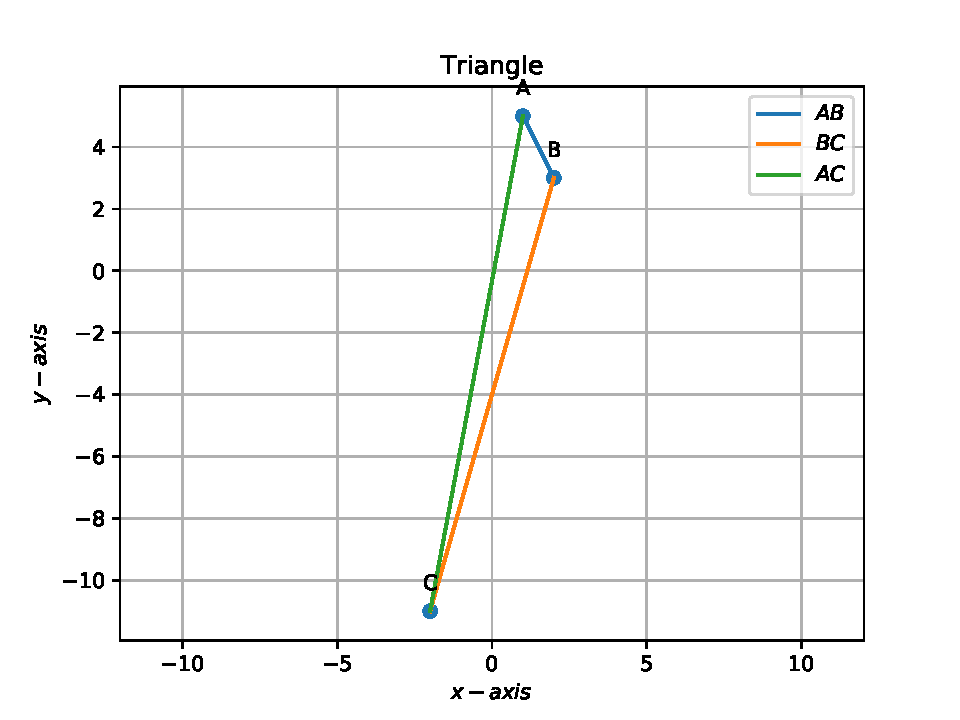
\includegraphics[width=\columnwidth]{chapters/10/7/1/3/figs/problem3.pdf}
	\end{center}
\caption{}
\label{fig:10/7/1/3Fig1}
\end{figure}


\item Show that the points $\vec{A}(1,2,7), \vec{B}(2,6,3)$ and $\vec{C}(3,10,-1)$ are collinear.
	\\
	\solution
		\iffalse
\documentclass[journal,12pt,twocolumn]{IEEEtran}
\usepackage{setspace}
\usepackage{gensymb}
\usepackage{xcolor}
\usepackage{caption}
\singlespacing
\usepackage{siunitx}
\usepackage[cmex10]{amsmath}
\usepackage{mathtools}
\usepackage{hyperref}
\usepackage{amsthm}
\usepackage{mathrsfs}
\usepackage{txfonts}
\usepackage{stfloats}
\usepackage{cite}
\usepackage{cases}
\usepackage{subfig}
\usepackage{longtable}
\usepackage{multirow}
\usepackage{enumitem}
\usepackage{mathtools}
\usepackage{listings}
\usepackage{tikz}
\usetikzlibrary{shapes,arrows,positioning}
\usepackage{circuitikz}
\let\vec\mathbf
\DeclareMathOperator*{\Res}{Res}
\renewcommand\thesection{\arabic{section}}
\renewcommand\thesubsection{\thesection.\arabic{subsection}}
\renewcommand\thesubsubsection{\thesubsection.\arabic{subsubsection}}

\renewcommand\thesectiondis{\arabic{section}}
\renewcommand\thesubsectiondis{\thesectiondis.\arabic{subsection}}
\renewcommand\thesubsubsectiondis{\thesubsectiondis.\arabic{subsubsection}}
\hyphenation{op-tical net-works semi-conduc-tor}

\lstset{
language=Python,
frame=single, 
breaklines=true,
columns=fullflexible
}
\begin{document}
\theoremstyle{definition}
\newtheorem{theorem}{Theorem}[section]
\newtheorem{problem}{Problem}
\newtheorem{proposition}{Proposition}[section]
\newtheorem{lemma}{Lemma}[section]
\newtheorem{corollary}[theorem]{Corollary}
\newtheorem{example}{Example}[section]
\newtheorem{definition}{Definition}[section]
\newcommand{\BEQA}{\begin{eqnarray}}
\newcommand{\EEQA}{\end{eqnarray}}
\newcommand{\define}{\stackrel{\triangle}{=}}
\newcommand{\myvec}[1]{\ensuremath{\begin{pmatrix}#1\end{pmatrix}}}
\newcommand{\mydet}[1]{\ensuremath{\begin{vmatrix}#1\end{vmatrix}}}
\bibliographystyle{IEEEtran}
\providecommand{\nCr}[2]{\,^{#1}C_{#2}} % nCr
\providecommand{\nPr}[2]{\,^{#1}P_{#2}} % nPr
\providecommand{\mbf}{\mathbf}
\providecommand{\pr}[1]{\ensuremath{\Pr\left(#1\right)}}
\providecommand{\qfunc}[1]{\ensuremath{Q\left(#1\right)}}
\providecommand{\sbrak}[1]{\ensuremath{{}\left[#1\right]}}
\providecommand{\lsbrak}[1]{\ensuremath{{}\left[#1\right.}}
\providecommand{\rsbrak}[1]{\ensuremath{{}\left.#1\right]}}
\providecommand{\brak}[1]{\ensuremath{\left(#1\right)}}
\providecommand{\lbrak}[1]{\ensuremath{\left(#1\right.}}
\providecommand{\rbrak}[1]{\ensuremath{\left.#1\right)}}
\providecommand{\cbrak}[1]{\ensuremath{\left\{#1\right\}}}
\providecommand{\lcbrak}[1]{\ensuremath{\left\{#1\right.}}
\providecommand{\rcbrak}[1]{\ensuremath{\left.#1\right\}}}
\theoremstyle{remark}
\newtheorem{rem}{Remark}
\newcommand{\sgn}{\mathop{\mathrm{sgn}}}
\newcommand{\rect}{\mathop{\mathrm{rect}}}
\newcommand{\sinc}{\mathop{\mathrm{sinc}}}
\providecommand{\abs}[1]{\left\vert#1\right\vert}
\providecommand{\res}[1]{\Res\displaylimits_{#1}} 
\providecommand{\norm}[1]{\lVert#1\rVert}
\providecommand{\mtx}[1]{\mathbf{#1}}
\providecommand{\mean}[1]{E\left[ #1 \right]}
\providecommand{\fourier}{\overset{\mathcal{F}}{ \rightleftharpoons}}
\providecommand{\ztrans}{\overset{\mathcal{Z}}{ \rightleftharpoons}}
\providecommand{\system}[1]{\overset{\mathcal{#1}}{ \longleftrightarrow}}
\newcommand{\solution}{\noindent \textbf{Solution: }}
\providecommand{\dec}[2]{\ensuremath{\overset{#1}{\underset{#2}{\gtrless}}}}
\let\StandardTheFigure\thefigure
\def\putbox#1#2#3{\makebox[0in][l]{\makebox[#1][l]{}\raisebox{\baselineskip}[0in][0in]{\raisebox{#2}[0in][0in]{#3}}}}
     \def\rightbox#1{\makebox[0in][r]{#1}}
     \def\centbox#1{\makebox[0in]{#1}}
     \def\topbox#1{\raisebox{-\baselineskip}[0in][0in]{#1}}
     \def\midbox#1{\raisebox{-0.5\baselineskip}[0in][0in]{#1}}

\vspace{3cm}
\title{Line Assignment}
\author{Gautam Singh}
\maketitle
\bigskip

\begin{abstract}
    This document contains the solution to Question 16 of Exercise 3 in Chapter
    10 of the class 12 NCERT textbook.
\end{abstract}

\begin{enumerate}
    \item Show that the points $\vec{A} = \myvec{1\\2\\7}$, $\vec{B} = 
    \myvec{2\\6\\3}$, and $\vec{C} = \myvec{3\\10\\-1}$ are collinear.


    \solution 
\fi
		Points $\vec{A}$, $\vec{B}$ and $\vec{C}$ are on a line if
    \begin{align}
        \textrm{rank}\myvec{\vec{A} & \vec{B} & \vec{C}} < 3
        \label{eq:chapters/12/10/3/16rank-collinear}
    \end{align}
    Substituting, we must find the rank of
    \begin{align}
        \vec{M} = \myvec{1&2&3\\2&6&10\\7&3&-1}
    \end{align}
    Using row reduction methods to bring $\mtx{M}$ into row-reduced echelon
    form,
    \begin{align}
        \myvec{1&2&3\\2&6&10\\7&3&-1}&\xleftrightarrow[]{R_2\rightarrow R_2-2R_1}
        \myvec{1&2&3\\0&2&4\\7&3&-1} \\
                &\xleftrightarrow[]{R_3\rightarrow R_3-7R_1}\myvec{1&2&3\\0&2&4\\0&-11&-22} \\
                &\xleftrightarrow[]{R_1\rightarrow R_1-R_2}\myvec{1&0&-1\\0&2&4\\0&-11&-22} \\
                &\xleftrightarrow[]{R_3\rightarrow R_3+\frac{11}{2}R_2}\myvec{1&0&-1\\0&2&4\\0&0&0}
                \label{eq:chapters/12/10/3/16row-red}
    \end{align}
    Clearly, the rank of $\mtx{M}$ is 2, and hence the given points are 
    collinear. 
    Fig. \ref{fig:chapters/12/10/3/163d-line}  verifies that the three points are indeed 
    collinear as claimed.
    \begin{figure}[!ht]
        \centering
        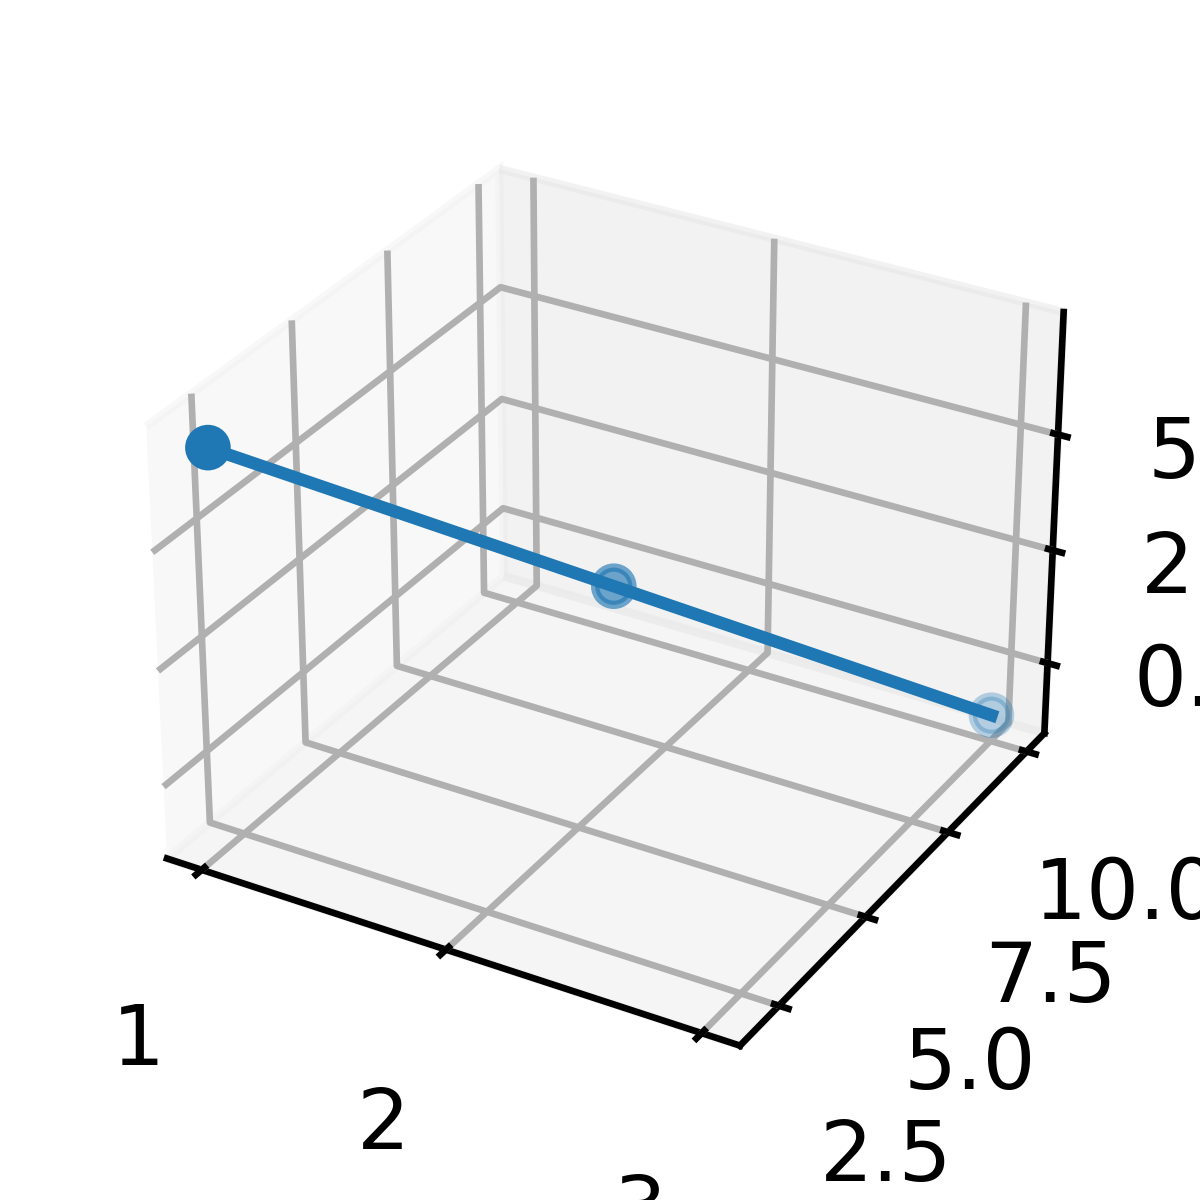
\includegraphics[width=\columnwidth]{chapters/12/10/3/16/figs/line_3d.png}
        \caption{Points $\vec{A}$, $\vec{B}$ and $\vec{C}$ are collinear.}
        \label{fig:chapters/12/10/3/163d-line}
    \end{figure}

\item Show that the vectors $2\hat{i}-3\hat{j}+4\hat{k}$ and $-4\hat{i}+6\hat{j}-8\hat{k}$ are collinear.
   \\ 
    \solution 
		\iffalse
\documentclass[12pt]{article}
\usepackage{graphicx}
\graphicspath{{./figs/}}{}
\usepackage{amsmath,amssymb,amsfonts,amsthm}
\newcommand{\myvec}[1]{\ensuremath{\begin{pmatrix}#1\end{pmatrix}}}
\providecommand{\norm}[1]{\lVert#1\rVert}
\usepackage{listings}
\usepackage{watermark}
\usepackage{titlesec}
\usepackage{caption}
\usepackage{extarrows}
\let\vec\mathbf
\lstset{
frame=single, 
breaklines=true,
columns=fullflexible
}
\thiswatermark{\centering \put(0,-105.0){
\includegraphics[scale=0.15]{/sdcard/IITH/vectors/12.10.2.11/figs/logo.png}} }
\title{\mytitle}
\title{
Assignment - 12.10.2.11
}
\author{Surajit Sarkar}
\begin{document}
\maketitle
\tableofcontents
\bigskip
\section{\textbf{Problem}}
Show that the vectors $2\hat{i}+3\hat{j}+4\hat{k}$ and $-4\hat{i}+6\hat{j}-8\hat{k}$ are collinear.
\section{\textbf{Solution}}
\fi
Let
\begin{align}
\vec{A}=\myvec{2\\3\\4},\vec{B}=\myvec{-4\\6\\-8}\\
 \end{align}
 Forming the collinearity matrix
 \begin{align}        
\myvec{\vec{A}^{\top}\\ \vec{B}^{\top}}=\myvec{2&-3&4\\-4&6&-8}
 \xleftrightarrow{\frac{1}{2}R_1\to R_1}\myvec{1&-\frac{3}{2}&2\\-4&6&-8}\\
\xleftrightarrow{-\frac{1}{4}R_2\leftarrow R_2}\myvec{1&-\frac{3}{2}&2\\1&\frac{3}{2}&2}
\xleftrightarrow{R_2-1R_1\to R_2}\myvec{1&-\frac{3}{2}&2\\0&0&0}
\end{align}
Thus, the rank of the matrix is 1 and the vectors are collinear.

\item Show that the points (2, 3, 4), (–1, –2, 1), (5, 8, 7) are collinear.
		\\
		\solution
		\iffalse
\documentclass[journal,12pt,twocolumn]{IEEEtran}
\usepackage{setspace}
\usepackage{gensymb}
\singlespacing
\usepackage[cmex10]{amsmath}
\usepackage{amsthm}
\usepackage{mathrsfs}
\usepackage{txfonts}
\usepackage{stfloats}
\usepackage{bm}
\usepackage{cite}
\usepackage{cases}
\usepackage{subfig}
\usepackage{longtable}
\usepackage{multirow}
\usepackage{enumitem}
\usepackage{mathtools}
\usepackage{steinmetz}
\usepackage{tikz}
\usepackage{circuitikz}
\usepackage{verbatim}
\usepackage{tfrupee}
\usepackage[breaklinks=true]{hyperref}
\usepackage{tkz-euclide}
\usetikzlibrary{calc,math}
\usepackage{listings}
    \usepackage{color}                                            %%
    \usepackage{array}                                            %%
    \usepackage{longtable}                                        %%
    \usepackage{calc}                                             %%
    \usepackage{multirow}                                         %%
    \usepackage{hhline}                                           %%
    \usepackage{ifthen}                                           %%
  %optionally (for landscape tables embedded in another document): %%
    \usepackage{lscape}     
\usepackage{multicol}
\usepackage{chngcntr}
\DeclareMathOperator*{\Res}{Res}
\renewcommand\thesection{\arabic{section}}
\renewcommand\thesubsection{\thesection.\arabic{subsection}}
\renewcommand\thesubsubsection{\thesubsection.\arabic{subsubsection}}

\renewcommand\thesectiondis{\arabic{section}}
\renewcommand\thesubsectiondis{\thesectiondis.\arabic{subsection}}
\renewcommand\thesubsubsectiondis{\thesubsectiondis.\arabic{subsubsection}}

% correct bad hyphenation here
\hyphenation{op-tical net-works semi-conduc-tor}
\def\inputGnumericTable{}                                 %%

\lstset{
frame=single, 
breaklines=true,
columns=fullflexible
}

\begin{document}


\newtheorem{theorem}{Theorem}[section]
\newtheorem{problem}{Problem}
\newtheorem{proposition}{Proposition}[section]
\newtheorem{lemma}{Lemma}[section]
\newtheorem{corollary}[theorem]{Corollary}
\newtheorem{example}{Example}[section]
\newtheorem{definition}[problem]{Definition}
\newcommand{\BEQA}{\begin{eqnarray}}
\newcommand{\EEQA}{\end{eqnarray}}
\newcommand{\define}{\stackrel{\triangle}{=}}

\bibliographystyle{IEEEtran}
\providecommand{\mbf}{\mathbf}
\providecommand{\pr}[1]{\ensuremath{\Pr\left(#1\right)}}
\providecommand{\qfunc}[1]{\ensuremath{Q\left(#1\right)}}
\providecommand{\sbrak}[1]{\ensuremath{{}\left[#1\right]}}
\providecommand{\lsbrak}[1]{\ensuremath{{}\left[#1\right.}}
\providecommand{\rsbrak}[1]{\ensuremath{{}\left.#1\right]}}
\providecommand{\brak}[1]{\ensuremath{\left(#1\right)}}
\providecommand{\lbrak}[1]{\ensuremath{\left(#1\right.}}
\providecommand{\rbrak}[1]{\ensuremath{\left.#1\right)}}
\providecommand{\cbrak}[1]{\ensuremath{\left\{#1\right\}}}
\providecommand{\lcbrak}[1]{\ensuremath{\left\{#1\right.}}
\providecommand{\rcbrak}[1]{\ensuremath{\left.#1\right\}}}
\theoremstyle{remark}
\newtheorem{rem}{Remark}
\newcommand{\sgn}{\mathop{\mathrm{sgn}}}
\providecommand{\abs}[1]{\left\vert#1\right\vert}
\providecommand{\res}[1]{\Res\displaylimits_{#1}} 
\providecommand{\norm}[1]{\left\lVert#1\right\rVert}
\providecommand{\mtx}[1]{\mathbf{#1}}
\providecommand{\mean}[1]{E\left[ #1 \right]}
\providecommand{\fourier}{\overset{\mathcal{F}}{ \rightleftharpoons}}
\providecommand{\system}{\overset{\mathcal{H}}{ \longleftrightarrow}}
\newcommand{\solution}{\noindent \textbf{Solution: }}
\newcommand{\cosec}{\,\text{cosec}\,}
\providecommand{\dec}[2]{\ensuremath{\overset{#1}{\underset{#2}{\gtrless}}}}
\newcommand{\myvec}[1]{\ensuremath{\begin{pmatrix}#1\end{pmatrix}}}
\newcommand{\mydet}[1]{\ensuremath{\begin{vmatrix}#1\end{vmatrix}}}
\numberwithin{equation}{subsection}
\makeatletter
\@addtoreset{figure}{problem}
\makeatother

\let\StandardTheFigure\thefigure
\let\vec\mathbf
\renewcommand{\thefigure}{\theproblem}



\def\putbox#1#2#3{\makebox[0in][l]{\makebox[#1][l]{}\raisebox{\baselineskip}[0in][0in]{\raisebox{#2}[0in][0in]{#3}}}}
     \def\rightbox#1{\makebox[0in][r]{#1}}
     \def\centbox#1{\makebox[0in]{#1}}
     \def\topbox#1{\raisebox{-\baselineskip}[0in][0in]{#1}}
     \def\midbox#1{\raisebox{-0.5\baselineskip}[0in][0in]{#1}}

\vspace{3cm}


\title{Assignment 1}
\author{Jaswanth Chowdary Madala}





% make the title area
\maketitle

\newpage

%\tableofcontents

\bigskip

\renewcommand{\thefigure}{\theenumi}
\renewcommand{\thetable}{\theenumi}


\begin{enumerate}


\textbf{Solution:} 
\fi
		The points given are,
\begin{align}
\vec{A} = \myvec{2\\3\\4}, \, \vec{B} = \myvec{-1\\-2\\1}, \,\vec{C}=\myvec{5\\8\\7}
\end{align}
%
To check whether the given points are collinear, we find the rank of the matrix 
%
\begin{align}
\myvec{\vec{A} & \vec{B} & \vec{C}}
=\myvec{2&-1&5\\3&-2&8\\4&1&7}
\xleftrightarrow[R_3 \leftarrow R_3 - 2R_1]{R_2 \leftarrow R_2 - \frac{3}{2}R_1}
\myvec{2&-1&5\\ \\0&-\frac{1}{2}&\frac{1}{2}\\ \\0&3&-3}\\
\xleftrightarrow{R_3 \leftarrow R_3 + 6R_2}
\myvec{2&-1&5\\\\0&-\frac{1}{2}&\frac{1}{2}\\\\0&0&0}
\end{align}
The matrix has a rank of 2. Hence the given points are collinear.




\item In each of the following, find the value of '$k$', for which the points are collinear.
\begin{enumerate}
\item $(7, –2), (5, 1), (3, k)$
\item $(8, 1), (k, – 4), (2, –5)$
\end{enumerate}
		\label{10/7/3/2}
\solution
		\iffalse
\documentclass[journal,10pt,twocolumn]{article}
\usepackage{graphicx}
\usepackage{caption} 
\usepackage{hyperref}
\usepackage[margin=0.5in]{geometry}
\usepackage{booktabs}
\usepackage{array}
\usepackage{amsmath}   % for having text in math mode
\usepackage{mathtools}
\usepackage{enumitem}
\usepackage{atbegshi}% http://ctan.org/pkg/atbegshi
\AtBeginDocument{\AtBeginShipoutNext{\AtBeginShipoutDiscard}}
\newcommand{\myvec}[1]{\ensuremath{\begin{pmatrix}#1\end{pmatrix}}}
\let\vec\mathbf
\newcommand{\mydet}[1]{\ensuremath{\begin{vmatrix}#1\end{vmatrix}}}
\providecommand{\brak}[1]{\ensuremath{\left(#1\right)}}
\newcommand{\solution}{\noindent \textbf{Solution: }}
\let\vec\mathbf
\begin{document}
\begin{center}
\title{\textbf{Properties of Collinear}}
\date{\vspace{-5ex}} %Not to print date automatically
\maketitle
\end{center}
\setcounter{page}{1}
\section{10$^{th}$ Maths - Chapter 7}
\textbf{This is Problem-2 from Exercise 7.3.2}
\item In each of the following find the value of ‘k’, for which the points are collinear.

\item (7, –2), (5, 1), (3, k) \\
\item (8, 1), (k, – 4), (2, –5).\\
\fi
\begin{enumerate}
\item 
Let
\begin{align}  
	\vec{A}&=\myvec{7 \\-2},
\vec{B}=\myvec{5 \\ 1},
\vec{C}=\myvec{3 \\ k}
\end{align}
Then
\begin{align}  
\vec{D} &=\brak{\vec{A}-\vec{B}} = \brak{\myvec{7 \\-2 } - \myvec{5 \\1 } } = \myvec{2 \\ -3 }\\
\vec{E} &= \brak{\vec{A}-\vec{C}} = \brak{\myvec{7 \\ -2 } - \myvec{3 \\k} } = \myvec{4 \\-2-k}
\end{align}
Forming the collinearlity matrix,
\begin{align}
\vec{F} &={\myvec{\vec{D}\\ \vec{E}}}
=
\myvec{
2 & -3
 \\
4 & -2-k 
}
\end{align}
yielding
\begin{align}
\label{eq:chapters/10/7/3/2/chem_balance_mat_row1}
 \xleftrightarrow[]{R_2 = R_2-2R_1}
\myvec{
2 & -3
\\
0 & -k+4
}
\end{align}
For the matrix to be rank 1, 
\begin{align}
 -k+4 =0
\implies k =4 
\end{align}
This is verified in Fig. 
	  \ref{fig:chapters/10/7/3/2/line1.pdf}.
\begin{figure}[h!]
	  \centering 
	  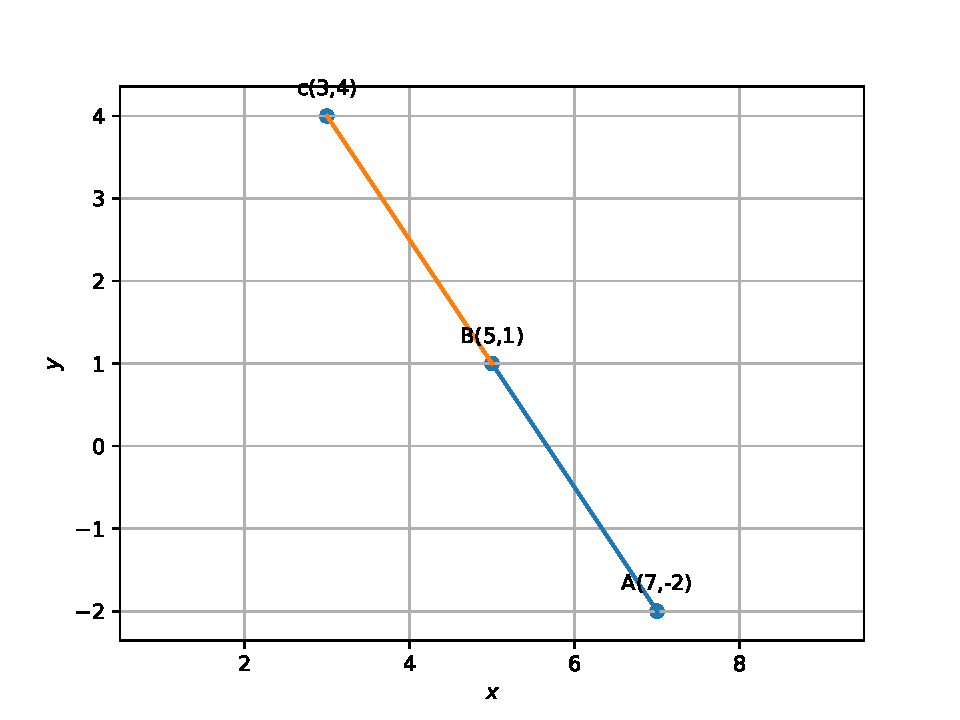
\includegraphics[width=\columnwidth]{chapters/10/7/3/2/figs/line1.pdf}
	  \caption{}
	  \label{fig:chapters/10/7/3/2/line1.pdf}
	  \end{figure} 	 		  
%
 \item In this case,
\begin{align}  
\vec{A}=\myvec{8 \\ 1},
\vec{B}=\myvec{k \\ -4},
\vec{C}=\myvec{2 \\ -5}.
\end{align}
Since
\begin{align}  
 \vec{D} &=\brak{\vec{A}-\vec{B}} = \brak{\myvec{8 \\1 } - \myvec{k \\-4 } } = \myvec{8-k \\ 5 }\\
\vec{E} &= \brak{\vec{A}-\vec{C}} = \brak{\myvec{8 \\ 1 } - \myvec{2 \\-5 } } = \myvec{6 \\6}
\end{align}
the collinearity matrix is
\begin{align}
\vec{F} &={\myvec{\vec{D}\\ \vec{E}}}
=
\myvec{
8-k & 5
 \\
6 & 6
}
\end{align}
yielding
\begin{align}
\label{eq:chapters/10/7/3/2/chem_balance_mat_row}
 \xleftrightarrow[]{R_1=\frac{R_1}{8-k}}
\myvec{
1& \frac{5}{8-k}
\\
6 & 6
}
\\
\xleftrightarrow[]{R_2 = R_2-6R_1}
\myvec{
1 & \frac{5}{8-k}
\\
\\
0 & 6-\frac{30}{8-k}
}
\end{align}
For 
the matrix to be rank 1,
\begin{align}
6-\frac{30}{8-k}&=0
\\
\implies k &=3
\end{align}
This is verified in Fig. 
	  \ref{fig:chapters/10/7/3/2/line2.png}
\begin{figure}[h]
	  \centering 
	  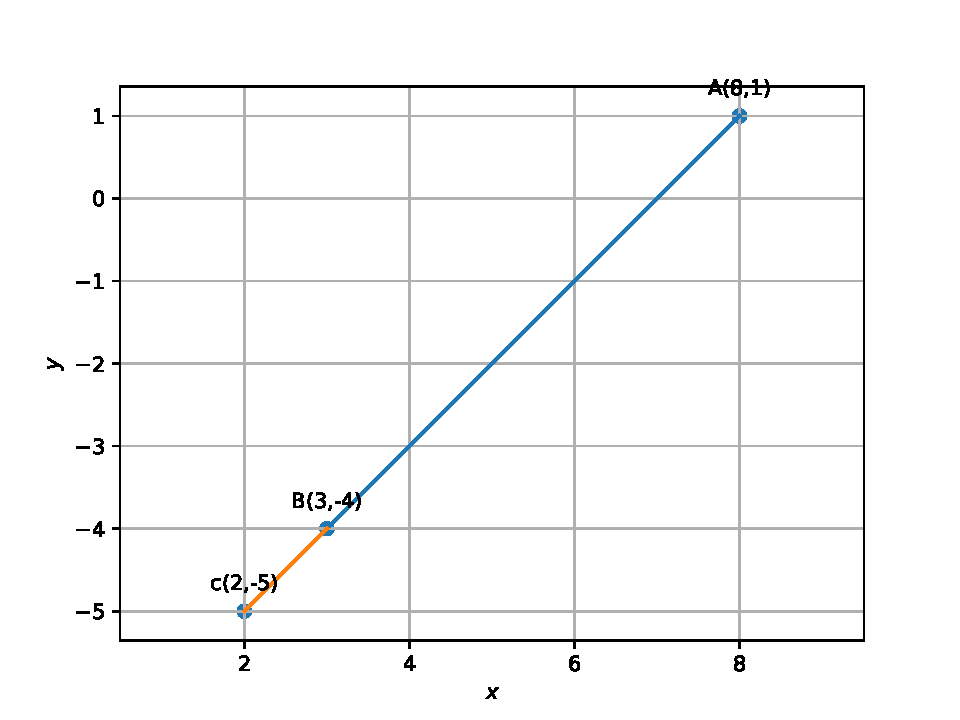
\includegraphics[width=\columnwidth]{chapters/10/7/3/2/figs/line2.pdf}
	  \caption{}
	  \label{fig:chapters/10/7/3/2/line2.png}
	  \end{figure}
\end{enumerate} 

\item Find a relation between $x$ and $y$ if the points $(x, y), (1, 2)$  and  $(7, 0)$ are collinear.
\\
\solution
	\iffalse
\documentclass[12pt]{article}
\usepackage{graphicx}
\usepackage{amsmath}
\usepackage{mathtools}
\usepackage{gensymb}

\newcommand{\mydet}[1]{\ensuremath{\begin{vmatrix}#1\end{vmatrix}}}
\providecommand{\brak}[1]{\ensuremath{\left(#1\right)}}
\providecommand{\norm}[1]{\left\lVert#1\right\rVert}
\newcommand{\solution}{\noindent \textbf{Solution: }}
\newcommand{\myvec}[1]{\ensuremath{\begin{pmatrix}#1\end{pmatrix}}}
\let\vec\mathbf

\begin{document}
\begin{center}
\textbf\large{CHAPTER-7 \\ COORDINATE GEOMETRY}
\end{center}
\section*{Excercise 7.4}

Q2. Find a relation between x and y if the points $\vec(x, y), \vec(1, 2) \text{ and } \vec(7, 0)$ are collinear.
\\
\solution
\\
The coordinates are given as
\fi
Let
	\begin{align}
	\vec{A} = \myvec{
		x\\
		y\\
		},
	\vec{B} = \myvec{
		1\\
		2\\
		},
	\vec{C} = \myvec{
		7\\
		0\\
		}
	\end{align}
	Then
	\begin{align}
\vec{D} &=\brak{\vec{A}-\vec{B}} = \brak{\myvec{x \\y } - \myvec{1 \\2 } } = \myvec{x-1 \\ y-2 }\\
\vec{E} &= \brak{\vec{A}-\vec{C}} = \brak{\myvec{x \\ y } - \myvec{7 \\0} } = \myvec{x-7 \\y}
\end{align}
Forming the collinearity matrix
\begin{align}
	\vec{F} &={\myvec{\vec{D}^{\top}\\ \vec{E}^{\top}}}
\end{align}
and performing row reduction,
\begin{align}
\label{eq:chapters/10/7/4/2chem_balance_mat_row}
\myvec{
x-1 & y-2
\\
x-7 & y
}
\xleftrightarrow[]{R_2 = R_2-R_1}
\myvec{
  x-1 & y-2
  \\
	  -6 & 2                 
	  }
	  \\
	\xleftrightarrow[]{R_2 = \frac{R_2}{-6}(x-1)-R_1}
\myvec{
x-1 & y-2
\\
	0 & -\frac{1}{3}(x-1)-(y-2)
}
\end{align}
For the rank of the matrix to be 1,
\begin{align}
	-\frac{1}{3}(x-1)-(y-2)&=0\\
	\implies \myvec{1 & 3}\vec{x} &=7	
\end{align}
For $x=-2, y=3$, see Fig. \ref{fig:chapters/10/7/4/2Fig} verifying that the points are collinear.
\begin{figure}[!h]
	\begin{center} 
	    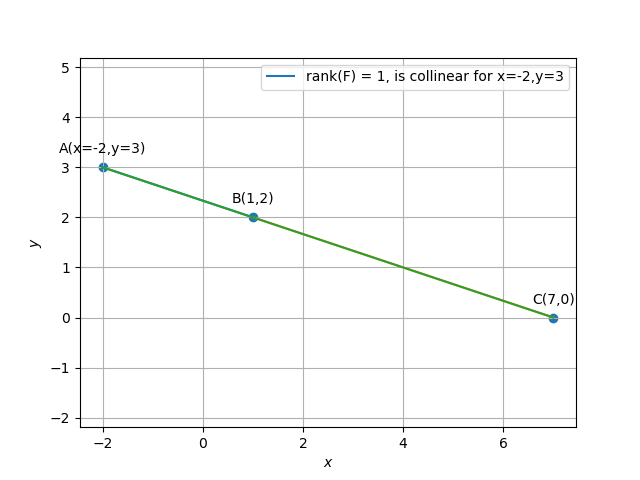
\includegraphics[width=\columnwidth]{chapters/10/7/4/2/figs/sc1.png}
	\end{center}
\caption{}
\label{fig:chapters/10/7/4/2Fig}
\end{figure}

\item If three points $(x, -1), (2, 1)$ and $(4, 5)$ are collinear, find the value of $x$.
\label{chapters/11/10/1/8}
\iffalse
\documentclass[10pt, a4paper]{article}
\usepackage[a4paper,outer=1.5cm,inner=1.5cm,top=1.75cm,bottom=1.5cm]{geometry}

\twocolumn
\usepackage{graphicx}

\usepackage{hyperref}
\usepackage[utf8]{inputenc}
\usepackage{amsmath}
\usepackage{physics}
\usepackage{amssymb}
\begin{document}
\title{Assignment-4}
\author{Name:C.CHANDANA\and Email :  \url{cheenepallichandana531@gmail.com}}
%\{ Wireless Communication (FWC)}
\date{30-sep-2022}
\maketitle



\section{Problem}
\fi
If three points $(x, -1), (2, 1)$ and $(4, 5)$ are collinear, find the value of $x$.
\\
\solution 
	\begin{figure}[!ht]
		\centering
 \includegraphics[width=\columnwidth]{chapters/11/10/1/8/figs/sline.png}
		\caption{}
		\label{fig:11/10/1/8}
  	\end{figure}
	\iffalse
\begin{center}
	\fi
	Let
\begin{align} \label{eq:11/10/1/8}
	\vec{A}=\myvec{ x\\ -1 },
	\vec{B}=\myvec{ 2\\ 1 },
\vec{C}=\myvec{ 4\\ 5 }.
\end{align}
Then
\begin{align}
\vec{A}-\vec{B}
	&=\myvec{ x-2\\ -2 }
	\\
\vec{A}-\vec{C}
	&=\myvec{ 4-x\\ 6 }
\end{align}
Forming the collinearity matrix
using 
	\eqref{eq:normal_line-collinear},
\begin{align} 
\myvec{ x-2 & -2\\ 4-x & 6  } 
	\xleftrightarrow[]{{R_1=3R_1+R-2}}
=\myvec{
2x-2 &0 \\ 
 4-x& 6
}
\end{align}

\iffalse

In the problem they have given that three points lie on a line, thats means these three points are collinear.\\

If  points on a line  are  collinear, rank of matrix is " 1 "then the vectors are in linearlydependent.\\
For 2 × 2 matrix Rank =1 means Determinant is 0.\\

Through pivoting,we obtain\\
\begin{align}
=\myvec{ x-2 & -2\\ 4-x & 6 \ } \\ 
\end{align}
\begin{align}
=\myvec{
x-2 &-2 \\ 
 4-x& 6
}\overset{R1=3R1+R2}{\rightarrow}
=\myvec{
2x-2 &0 \\ 
 4-x& 6
}
\end{align} 
\fi
	If the rank of the matrix is 1, any one of the rows must be zero. So, making the first element in the above matrix 0,
\begin{align}
x=1
\end{align} 

\iffalse

\begin{align}\label{eq:11/10/1/8}
x=1 \\
\end{align} 

Hence proved.\\
\section{Construction}
 \begin{figure}[h]
\centering
\includegraphics[scale=0.4]{sline.png} 
\caption{}
\end{figure}
\section{Code}
*Verify the above proofs in the following code.\\
\framebox{
\url{https://github.com/chandana531/FWC/tree/main/matrix/line}}	
\bibliographystyle{ieeetr}
\end{document}
\fi

\item If three points $(h, 0), (a, b)$ and $(0, k)$ lie on a line, 
show that 
\begin{align}
\frac{a}{h}+\frac{b}{k}=1
\end{align}
\label{chapters/11/10/1/13}
\iffalse
\documentclass[10pt, a4paper]{article}
\usepackage[a4paper,outer=1.5cm,inner=1.5cm,top=1.75cm,bottom=1.5cm]{geometry}

\twocolumn
\usepackage{graphicx}

\usepackage{hyperref}
\usepackage[utf8]{inputenc}
\usepackage{amsmath}
\usepackage{physics}
\usepackage{amssymb}
\begin{document}
\title{Assignment-4}
\author{Name:A.SUSI\and Email :  \url{susireddy9121@gmail.com}}
%\{ Wireless Communication (FWC)}
\date{30-sep-2022}
\maketitle



\section{Problem}
\fi
\solution 
\iffalse
\section{Solution}
\begin{center}
The input given 
\boldmath
\fi 
Let
\begin{align} 
\vec{A}=\myvec{ h\\ 0 },
\vec{B}=\myvec{ a\\ b },
\vec{C}=\myvec{ 0\\ k }
\end{align}
Forming the matrix in 
	\eqref{eq:normal_line-collinear}, we obtain, upon row reduction
	\iffalse
\begin{align}
\myvec{ h-a & -b\\ h & -k  } 
\end{align}
Using row reduction, 


In the problem they have given that three points lie on a line, thats means these three points are collinear.\\
If  points on a line  are  collinear, rank of matrix is "1"then the vectors are in linearlydependent.\\
For 2 × 2 matrix Rank =1 means Determinant is 0.\\
Through pivoting,we obtain\\
\fi
\begin{align}\label{eq:}
\myvec{ h-a & -b\\ h & -k  }  
	\xleftrightarrow[]{{\frac{R_1}{h-a}}}\myvec{
1 &\frac{-b}{h-a} \\ 
 h& -k
}
	\\
	\xleftrightarrow[]{R_2\rightarrow R_2-hR_1}
\myvec{
1 &\frac{-b}{h-a} \\ 
 0&-k+\frac{bh}{h-a} 
}
\end{align} 
For obtaining a rank 1 matrix, 
\iffalse

if the rank of the matrix is 1 means any one of the row must be zero.So, making the last element in the matrix to 0.\\
\fi
\begin{align}
	-k+\frac{bh}{h-a}&=0
	\\
	\implies \frac{a}{h}+\frac{b}{k}&=1 
\end{align} 
upon simplification.
\iffalse

Hence proved.\\
\section{Construction}
 \begin{figure}[H]
\centering
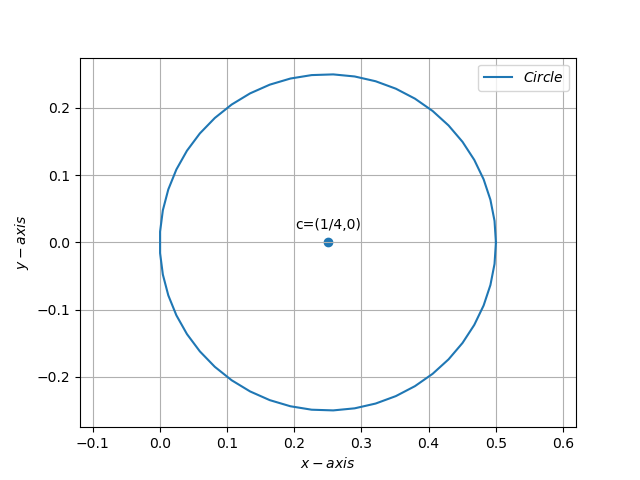
\includegraphics[width=0.75\columnwidth]{fig.png} 
\caption{}
\end{figure}
\section{Code}
*Verify the above proofs in the following code.\\
\framebox{
\url{https://github.com/Susi9121/FWC/tree/main/matrix/line}}	
\bibliographystyle{ieeetr}
\end{document}
\fi

\item Show that the points A (1, -2, -8), B (5, 0, -2) and C (11, 3, 7) are collinear, and find the ratio in which B divides AC.\\
\item lf the points $\vec{A}(1,2),\vec{0}(0,0)\text{ and }\vec{C}(a,b)$ are collinear,then
\begin{enumerate}
\item a=b
\item a=2b
\item 2a=b
\item a=-b
\end{enumerate}
\end{enumerate}
True/false
\begin{enumerate}[label=\thesection.\arabic*,ref=\thesection.\theenumi,resume*]
	\item $\triangle\vec{A}\vec{B}\vec{C}$ with vertices $\vec{A}(-2,0), \vec{B}(2,0) \text{ and }\vec{C}(0,2)$ is similar to $\triangle \vec{DEF}$  with vertices $\vec {D}(-4,0),\vec{E}(4,0)  \text{ and } \vec{F}(0,4)$  
	\item Point $ (-4,2)$ lies on the line segment joining the points $ \vec{A}(-4,6) \text{ and } \vec{B}(-4,-6)$
 \item The points $(0,5),(0,-9)\text{ and }(3,6)$ are collinear
\item Points $\vec{A}(3,1), \vec{B}(12,-2) \text{ and } \vec {C}(0,2)$ cannot be the vertices of a triangle
\item Find the value of $m$ if the points $(5,1),(-2,-3) \text{ and }(8,2m)$ are collinear.
\item Find the values of k if the points $\vec{A}(k+1,2k),\vec{B}(3k,2k+3)\text{ and }\vec{C}(5k-1,5k)$ are collinear
\item Using vectors, find the value of $k$ such that the points $(k,-10,3)$, $(1,-1,3)$ $\text{ and }$ $(3,5,3)$ are collinear.
\end{enumerate}

\subsection{Length}
\begin{enumerate}[label=\thesubsection.\arabic*,ref=\thesubsection.\theenumi]
\item Compute the magnitude of the following vectors:
\begin{align}
	\vec{a}&=\hat{i}+\hat{j}+\hat{k}
	\\
	\vec{b}&=2\hat{i}-7\hat{j}-3\hat{k}
	\\
	\vec{c}&=\frac{1}{\sqrt{3}}\hat{i}+\frac{1}{\sqrt{3}}\hat{j}-\frac{1}{3}\hat{k}
\end{align}
    \solution 
		Let 
\begin{align}
	\vec{a} = \myvec{1\\1\\1} , \vec{b} = \myvec{2\\ -7 \\ 3}, 
\vec{c} = \myvec{\dfrac{1}{\sqrt{3}}\\[2ex] \dfrac{1}{\sqrt{3}} \\[2ex] -\dfrac{1}{\sqrt{3}}} 
\label{eq:chapters/12/10/2/1/1}
\end{align}
Then
\begin{align}
	\norm{\vec{a}}&=\sqrt{\vec{a}^{\top}\vec{a}}=\sqrt{3}, 
	\label{eq:chapters/12/10/2/1/3}
	\\ \norm{\vec{b}}&=\sqrt{\vec{b}^{\top}\vec{b}}= \sqrt{62}, 
	\label{eq:chapters/12/10/2/1/4}
	\\ \norm{\vec{c}}&=\sqrt{\vec{c}^{\top}\vec{c}}	
=1
	\label{eq:chapters/12/10/2/1/5}
\end{align}




\item Find the value of x for which $x(\hat{i}+\hat{j}+\hat{k})$ is a unit vector.\\
	\solution
		\begin{align} 
\because
\vec{x}=x\myvec{1\\1\\1},
\norm{\vec{x}}=1
\implies 
x\sqrt{3}=1
\\
	\text{or, }x=\frac{1}{\sqrt{3}}
\end{align}   

\item If $\vec{a}=\vec{b}+\vec{c}$, then is it true that $|\vec{a}|=|\vec{b}|+|\vec{c}|$? Justify your answer.\\
	\solution
		\iffalse
\documentclass[journal,12pt,twocolumn]{IEEEtran}
\usepackage{graphicx}
\graphicspath{{./figs/}}{}
\usepackage{amsmath,amssymb,amsfonts,amsthm}
\newcommand{\myvec}[1]{\ensuremath{\begin{pmatrix}#1\end{pmatrix}}}
\providecommand{\norm}[1]{\lVert#1\rVert}
\usepackage{listings}
\usepackage{watermark}
\usepackage{titlesec}
\usepackage{caption}
\newcommand{\mydet}[1]{\ensuremath{\begin{vmatrix}#1\end{vmatrix}}}
\let\vec\mathbf
\lstset{
frame=single, 
breaklines=true,
columns=fullflexible
}
\thiswatermark{\centering \put(0,-105.0){
\includegraphics[scale=0.15]{/sdcard/IITH/vectors/12.10.5.4/figs/logo.png}} }
\title{\mytitle}
\title{
Assignment - 12.10.5.4
}
\author{Surajit Sarkar}
\begin{document}
\maketitle
\tableofcontents
\bigskip
\section{\textbf{Problem}}
if $\vec{a}=\vec{b}+\vec{c}$, then is true that $|\vec{a}|=|\vec{b}|+|\vec{c}|$?
Justify your answer .
\section{\textbf{Solution}}
Given
\begin{align}
    \vec{a}=\vec{b}+\vec{c}
\end{align}
\fi
Let
\begin{align}
    \vec{b}=\myvec{1\\2\\3},\vec{c}=\myvec{2\\-1\\-2}
\end{align}
Then
\begin{align}
	\vec{a}&=\vec{b}+\vec{c}
    =\myvec{3\\1\\1}
    \\
	\implies
    \norm{\vec{a}}
    &=\sqrt{11},\,
    \norm{\vec{b}}    =\sqrt{14},\,
    \norm{\vec{c}}
    =3.
\end{align}
Thus
\begin{align}
	\norm{\vec{a}}\ne\norm{\vec{b}}+\norm{\vec{c}}
\end{align}


\item If $\overrightarrow {a}$ is a nonzero vector of magnitude `a' and $\lambda$ a nonzero scalar, then $\lambda\overrightarrow {a}$ is a unit vector if
\begin{enumerate} 
\item $\lambda=1$ 
\item $\lambda=-1$
\item $a=\abs{\lambda}$
\item $a=1/\abs{\lambda}$  
\end{enumerate}
\item A vector $\vec{r}$ is inclined at equal angles to the three axis. If the magnitude of $\vec{r}$ is $2\sqrt{3}$ units, find $\vec{r}$.
\item Find the unit vector in the direction of sum of vectors $\vec{a}$= $2\hat{i}-\hat{j}+\hat{k}$ $\text{ and }$ $\vec{b}=2\hat{j}+\hat{k}$.
\item If $\vec{a}$=$\hat{i}+\hat{j}+2\hat{k}$ $\text{ and }$ $\vec{b}$=$2\hat{i}+\hat{j}-2\hat{k}$, find the unit vector in the direction of
	\begin{enumerate}
		\item 6$\vec{a}$   
		\item 2$\vec{a}$-$\vec{b}$
	\end{enumerate}

\item Find a unit vector in the direction of $\overline{PQ} $, where P and Q have co-ordinates(5,0,8) and (3,3,2),respectively.
\item The vector in the direction of the vector $\hat{i}-2\hat{j}+2\hat{k}$ that has magnitude 9 is
	\begin{enumerate}
\item $\hat{i}-2\hat{j}+2\hat{k}$
\item $\hat{i}-2\hat{j}$
\item $3(\hat{i}-2\hat{j}+2\hat{k})$
\item $9(\hat{i}-2\hat{j}+2\hat{k})$
\end{enumerate}
\item If $|\vec{a}|=4$ $\text{and}$  $-3\leq\lambda\leq2$, then the range of $|\lambda\vec{a}|$ is
	\begin{enumerate}
\item $\left[0,8\right]$
\item $\left[-12,8\right]$
\item $\left[0,12\right]$	
\item $\left[8,12\right]$
\end{enumerate}
\item The values of $k$ for which $\abs{\vec{ka}}$ $<$ $\abs{\vec{a}}$ $\text{and}$ $k\vec{a}$+$\dfrac{1}{2}$ $\vec{a}$ is parallel to $\vec{a}$ holds true are \rule{1cm}{0.15mm}.
\item If $\abs{\vec{a}}$ = $\abs{\vec{b}}$, then necessarily it implies $\vec{a}=\pm\vec{b}$.

\item The direction cosines of the vector $(2\hat{i}+2\hat{j}-\hat{k})$ are \noindent\rule{2cm}{0.4pt}.

\item Position vector of point P is a vector whose intial point is origin.

\end{enumerate}

%
\newpage
\subsection{Direction}
\begin{enumerate}[label=\thesubsection.\arabic*,ref=\thesubsection.\theenumi]
\item Find the slope of a line, which passes through the origin and the mid point of the line segment joining the points $\vec{P}$(0,-4) and $\vec{B}$(8,0).
\label{chapters/11/10/1/5}
	\\
	\solution
The mid point of $PB$ is
\begin{align}
\vec{M} =\frac{1}{2}(\vec{P}+\vec{B})
	= \myvec{4 \\ -2}  
\end{align}
which, from  \eqref{eq:dir-vec}, is equal to the direction vector of $OM$, where $\vec{O}$ is the origin.
\begin{align}
\because \vec{M} \equiv
	 \myvec{1 \\ -\frac{1}{2}},
	m = -\frac{1}{2}
\end{align}
which, from \eqref{eq:dir-vec},  is the desired slope.
See 
		\figref{fig:11/10/1/5}.
	\begin{figure}[H]
		\centering
 %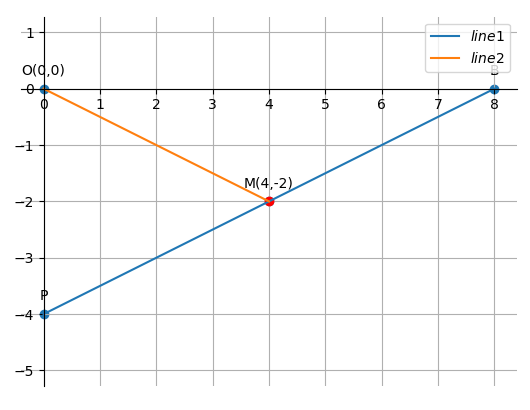
\includegraphics[width=0.75\columnwidth]{chapters/11/10/1/5/figs/line.png}
 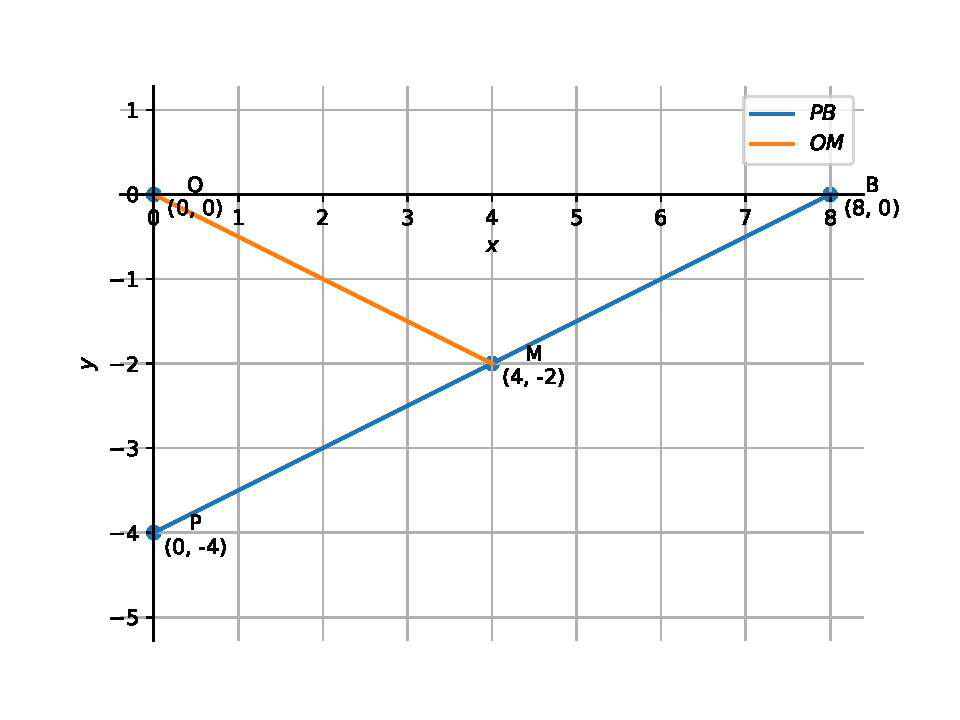
\includegraphics[width=0.75\columnwidth]{chapters/11/10/1/5/figs/fig.pdf}
		\caption{}
		\label{fig:11/10/1/5}
  	\end{figure}

\item A line passes through $A(x_1,y_1)$ and $B(h,k)$. If slope of the line is m, show that $(k-y_1)=m(h-x_1)$.
\label{chapters/11/10/1/12}
\\
\solution 
The direction vector
\begin{align}
	\vec{B}-\vec{A}
	=
	\myvec{
  h-x_1\\
  k-y_1
  }
   \equiv
	\myvec{
1\\
	\frac{ k-y_1}{h-x_1}
  }
  \\
	\implies m = 
	\frac{ k-y_1}{h-x_1},
\end{align}
yielding the desired result.

\item For given vectors, $\vec{a}=2\hat{i}-\hat{j}+2\hat{k}$ and $\vec{b}=-\hat{i}+\hat{j}-\hat{k}$ , find the unit vector in the
direction of the vector $\vec{a}+\vec{b}$.
        \label{prob:12/10/2/9}
\\
    \solution 
		\begin{align}
	\because \vec a + \vec b = \myvec{ 2\\-1\\2 } + \myvec{ -1\\1\\-1 },
= \myvec{ 1\\0\\1 },
\\
	\norm{\vec a + \vec b } = \sqrt{2}
	\\
	\implies \frac{\vec a + \vec b }{\norm{\vec a + \vec b }} = \frac{1}{\sqrt{2}}\myvec{ 1\\0\\1 }
\end{align}
which, from  \eqref{eq:unit-vec} is the desired the unit vector.
		





\item Find a vector of magnitude 5 units, and parallel to the resultant of the vectors $\vec{a}=2\hat{i}+3\hat{j}-\hat{k}$ and $\vec{b}=\hat{i}-2\hat{j}+\hat{k}$.\\
\item If $\vec{a}=\hat{i}+\hat{j}+\hat{k}, \vec{b}=2\hat{i}-\hat{j}+3\hat{k}$ and $\vec{c}=\hat{i}-2\hat{j}+\hat{k}$, find a unit vector parallel to the vector $2\vec{a}-\vec{b}+3\vec{c}$.\\
	\solution
		\begin{align}
2\vec{a}-\vec{b}+3\vec{c}=\myvec{3\\-3\\2}
\implies
\frac{2\vec{a}-\vec{b}+3\vec{c}}{\norm{2\vec{a}-\vec{b}+3\vec{c}}}
=\frac{1}{\sqrt{22}}\myvec{3\\-3\\2}
\end{align}


\item Find a vector in the direction of vector $5\hat{i}-\hat{j}+2\hat{k}$ which has magnitude 8 units.
        \label{prob:12/10/2/10const}
   \\ 
    \solution 
		Let the required vector be 
    \begin{align}
c\myvec{5\\-1\\2}.
    \end{align}
    From the given information, 
    \begin{align}
        \norm{c\myvec{5\\-1\\2\\}} =  8 \\
	    \implies \abs{c} = \frac{4\sqrt{30}}{15}
        \label{eq:12/10/2/10const}
    \end{align}


\item Find the unit vector in the direction of the vector $\vec{a}=\hat{i}+\hat{j}+2\hat{k}$.
\item Find the unit vector in the direction of vector $\overrightarrow{PQ}$ , where $\vec{P}$ and $\vec{Q}$ are the points
(1, 2, 3) and (4, 5, 6), respectively.
	\item 
Find a vector of magnitude 5 units, and parallel to the resultant of the vectors $\vec{a} = 2\hat{i}+3\hat{j}-\hat{k}$ and $\vec{b} = \hat{i}-2\hat{j}+\hat{k}$.
\\
\solution
		\begin{align}
\because     \Vec{a}=\myvec{
        2\\3\\-1
    },\Vec{b}=\myvec{
        1\\-2\\1
    }\\
	\vec{a}+\vec{b}=\myvec{
        3\\1\\0
    }
    \implies
	\norm{\vec{a}+\vec{b}}=\sqrt{10}
\end{align}
From problem
        \ref{prob:12/10/2/9},
the unit vector in the direction of 
${\vec{a}+\vec{b}}$
is
\begin{align}
	\frac{{\vec{a}+\vec{b}}}{\norm{\vec{a}+\vec{b}}}
=\frac{1}{\sqrt{10}}\myvec{
        3\\1\\0
    }
\end{align}
The desired vector can then be expressed as
\begin{align}
\pm\frac{5}{\sqrt{10}}\myvec{
        3\\1\\0
    }
\end{align}


	\item If a line makes angles $90\degree,135\degree,45\degree$ with x,y and z-axis respectivly. Find its direction cosines.
		\\
		\solution
				From \eqref{eq:dir-vec-3d},
the direction vector is
\begin{align}
\vec{A}=\myvec{\cos 90\degree\\ \cos 135\degree\\ \cos 45\degree}=\myvec{0\\-\frac{1}{\sqrt{2}}\\ \frac{1}{\sqrt{2}}}
\end{align}

\item Find the direction cosines of the vector joining the points $\vec{A}$ (1, 2, –3) and
$\vec{B}$(–1, –2, 1), directed from $\vec{A}$ to $\vec{B}$.
	\\
    \solution 
		The unit vector  in the direction of AB is 
\begin{align}
	\frac{\vec{B}-\vec{A}}{\norm{\vec{B}-\vec{A}}}
	= \frac{1}{3}{\myvec{-1\\-2\\2}}
\end{align}
and the direction cosines are the elements of the above vector.

\item Show that the vector $\hat{i}+\hat{j}+\hat{k}$ is equally inclined to the axes OX, OY and OZ.
	\\
\solution
		Since all entries of the given vector 
\begin{align}
\myvec{1\\1\\1}
\end{align}
are equal, it is equally inclined to the axes.

\item If a line has the direction ratios –18, 12, –4, then what are its direction cosines?
		\\
		\solution
		Let
\begin{align}
	\vec{A} =\myvec{-18\\12\\-4}
\end{align}
Then the unit direction vector of the line is
\begin{align}
		\frac{\vec{A}}{\norm{\vec{A}}} =
\myvec{\frac{-9}{11}\\[2pt] \frac{6}{11}\\[2pt] \frac{-2}{11}}
\end{align}

	\item Find the direction cosines of the sides of a triangle whose vertices are $\myvec{3\\ 5\\-4 }$, $\myvec{ -1\\1 \\2 }$ and $\myvec{-5 \\-5 \\-2 }$.
		\\
		\solution
		Let the vertices be
\begin{align}
\vec{A} = \myvec{3\\5\\-4},
\vec{B} = \myvec{-1\\1\\2},
\vec{C} = \myvec{-5\\-5\\-2}
\end{align}
%
The direction vectors of the sides are,
\begin{align}
\vec{A} - \vec{B} = \myvec{4\\4\\-6} = \vec{m_1},
\vec{B} - \vec{C} = \myvec{4\\6\\4} = \vec{m_2}, 
\\
\vec{C} - \vec{A} = \myvec{-8\\-10\\2} =\vec{m_3},
\end{align}
%
The corresponding unit vectors are then obtained as
\begin{align}
 \myvec{ \frac{2}{\sqrt{17}} \\[1pt] \frac{2}{\sqrt{17}} \\[1pt] \frac{-3}{\sqrt{17}} },
 \myvec{ \frac{2}{\sqrt{17}} \\[1pt] \frac{3}{\sqrt{17}} \\[1pt] \frac{2}{\sqrt{17}} }, 
 \myvec{ \frac{-4}{\sqrt{42}} \\[1pt] \frac{-5}{\sqrt{42}} \\[1pt] \frac{1}{\sqrt{42}} } 
\end{align}

\item Find the direction cosines of the vector $\hat{i}+2\hat{j}+3\hat{k}$.
	\\
    \solution 
		The unit vector in the direction of the given vector is 
\begin{align}
	\vec{A} =\frac{1}{\sqrt{14}}\myvec{1\\2\\3}
\end{align}

    \item Find the direction cosines of a line which makes equal angles with the coordinate
    axes.
		\\
		\solution
		Let $\alpha$ be the angle made by the line with the axes.  The unit direction vector can be expressed as
    \begin{align}
	    \vec{x} &= \myvec{\cos\alpha\\\cos\alpha\\\cos\alpha} 
	\implies
	    \norm{\vec{x}}  = 1
	\\
	    \text{or, }\cos\alpha &= \frac{1}{\sqrt{3}}
    \end{align}
    Thus the unit direction vector  of the given line is 
    \begin{align}
	    \vec{x} = \frac{1}{\sqrt{3}} \myvec{1 \\ 1 \\ 1} 
\end{align}
    

\item Write down a unit vector in XY-plane, making an angle of 30$\degree$ with the positive direction of x-axis.\\
\end{enumerate}

\newpage
\subsection{Scalar Product}
\begin{enumerate}[label=\thesubsection.\arabic*,ref=\thesubsection.\theenumi]
\item Find the angle between two vectors $\overrightarrow{a}$ and $\overrightarrow {b} $ with magnitudes $\sqrt{3}$ and 2 respectively having $\overrightarrow {a}\cdot\overrightarrow {b}=\sqrt{6}$.
		\label{prob:12/10/3/1/inner}
	\\
	\solution
		From the given information,
\begin{align}
\norm{\vec{a}}=\sqrt{3},
\norm{\vec{b}}= 2,
{\vec{a}^{\top}}{\vec{b}}=\sqrt{6}  
\\
\implies \cos\theta=\frac{{\vec{a}^{\top}}{\vec{b}}}{\norm{\vec{a}}\norm{\vec{b}}}
=\frac{1}{\sqrt{2}}\\
	\text{or, }\theta={45}\degree
\end{align}

\item Find the angle between the the vectors $\hat{i}-2\hat{j}+3\hat{k}$ and $3\hat{i}-2\hat{j}+\hat{k}$.
	\\
	\solution
		Let 
\begin{align}
	\vec{a} = \myvec{1\\-2\\3} , \vec{b} = \myvec{3\\ -2 \\ 1},
\end{align}
		From problem \ref{prob:12/10/3/1/inner},
\begin{align}
\cos\theta=\frac{\vec{a}^{\top}\vec{b}}{\norm{\vec{a}}\norm{\vec{b}}}
	= \frac{10}{\sqrt{14}\times \sqrt{14}}= \frac{5}{7}
\end{align}

\item Find $\abs{\overrightarrow {a}}$ and $\abs{\overrightarrow {b}}$, if ($\overrightarrow {a}+\overrightarrow {b}). (\overrightarrow {a}-\overrightarrow {b})=8$ and $\abs{\overrightarrow {a}}=8\abs{\overrightarrow {b}}$.
	\\
	\solution
		\begin{align}
\because \brak{\vec{a}+\vec{b}}^\top\brak{\vec{a}-\vec{b}}=8,
\norm{\vec{a}} &= 8\norm{\vec{b}},\\
\norm{\vec{a}}^2-\norm{\vec{b}}^2&=8\\
\implies\norm{8\vec{b}}^2-\norm{\vec{b}}^2&=8\\
\implies \norm{\vec{b}}&=\frac{2\sqrt{2}}{3\sqrt{7}}
\end{align}
Thus, 
\begin{align}
\norm{\vec{a}}&=8\norm{\vec{b}}
=\frac{16\sqrt{2}}{3\sqrt{7}}
\end{align}

\item Evaluate the product $(3\overrightarrow {a}-5\overrightarrow {b})\cdot (2\overrightarrow {a}+7\overrightarrow {b})$.
	\\
	\solution
		\begin{multline}
    \brak{3\vec{a}-5\vec{b}}^{\top}\brak{2\vec{a}+7\vec{b}}= 3\vec{a}^{\top}\brak{2\vec{a}+7\vec{b}} - 5\vec{b}^{\top}\brak{2\vec{a}+7\vec{b}}
    \\
     =6\norm{\vec{a}}^2-35\norm{\vec{b}}^2+11\vec{a}^{\top}\vec{b}
\end{multline}

\item Find the magnitude of two vectors $\overrightarrow {a}$ and $\overrightarrow {b}$, having the same magnitude and such that the angle between them is $60\degree$ and their scalar product is $\frac{1}{2}$.
	\\
	\solution
		Given 
\begin{align}
	\norm{\vec{a}}= \norm{\vec{b}}, {\cos\theta} = \frac{1}{2}, 
	\vec{a}^{\top}{\vec{b}} = \frac{1}{2},  \\
\implies 
	\frac{1}{2} = \frac{\frac{1}{2}}{\norm{\vec{a}}^2}
\implies \norm{\vec{a}}
= \norm{\vec{b}}=1
\end{align}
by using  the definition of the scalar product.

\item Find $\abs{\overrightarrow {x}}$, if for a unit vector $\overrightarrow {a}, (\overrightarrow {x}-\overrightarrow {a})\cdot (\overrightarrow {x}+\overrightarrow {a}$)=12.
	\\
\solution 
		From the given information,
\begin{align}
  \label{eq:12/10/3/9det2f}
  \brak{\vec{x}-\vec{a}}^\top\brak{\vec{x}+\vec{a}} &= 12 \\
  \implies \norm{\vec{x}}^{2} - \norm{\vec{a}}^{2} &= 12 \\
\implies   
	\norm{\vec{x}} &= \sqrt{13}
\end{align}

\item If the vertices $A,B,C$ of a triangle $ABC$ are (1,2,3), (-1,0,0), (0,1,2), respectively, then find  $\angle{ABC}$.
	\\
	\solution
		From the given information, 
\begin{align}
\vec{A} - \vec{B} &= \myvec{2\\2\\3},
\vec{C} - \vec{B} = \myvec{1\\1\\2}\\
	\implies \angle{ABC} &= \cos^{-1}{\frac{\brak{\vec{A} -\vec{B}}^{\top}\brak{\vec{C}-\vec{B}}}{\norm{\vec{A} -\vec{B}}  \norm{\vec{C}-\vec{B}}}}\\
&= \cos^{-1}{\frac{10}{\sqrt{102}}}\\
\end{align}




\item Find a unit vector perpendicular to each of the vector $\overrightarrow{a}+\overrightarrow{b}\text{ and }\overrightarrow{a}-\overrightarrow{b},\text{ where } \overrightarrow{a}=3\hat{i}+2\hat{j}+2\hat{k}\text{ and } \overrightarrow{b}=\hat{i}+2\hat{j}-2\hat{k}$. 
	\\
		\solution
		Let the desired vector be $\vec{x}$.  Then, 
\begin{align} 
\myvec{\vec{a}+\vec{b}& \vec{a}-\vec{b}}^\top\vec{x}=0\\
	\label{eq:12/10/4/2/given}
\end{align}
\begin{align}
	\because 
	\vec{a}+\vec{b}= \myvec{\vec{a} & \vec{b}}\myvec{1 \\ 1}
	\\
	\vec{a} - \vec{b}= \myvec{\vec{a} & \vec{b}}\myvec{1 \\ -1}, 
\end{align}
	\eqref{eq:12/10/4/2/given}
	can be expressed as 
\begin{align}
	\cbrak{\myvec{\vec{a} & \vec{b}}\myvec{1 & 1\\ 1 & -1}}^\top\vec{x}=0\\
\implies 	\myvec{1 & 1\\ 1 & -1}^\top\myvec{\vec{a} & \vec{b}}^\top\vec{x}=0
\\
\implies 	\myvec{1 & 1\\ 1 & -1}\myvec{1 & 1\\ 1 & -1}^\top\myvec{\vec{a} & \vec{b}}^\top\vec{x}=0
\\
	\text{or, }
\myvec{\vec{a} & \vec{b}}^\top\vec{x}=0
\end{align}
which can be expressed as 
\begin{align} 
\myvec{
3&2&2\\
1&2&-2
}
	\xleftrightarrow[R_2 = \frac{R_2}{4}]{R_2=3R_2-R_1}
\myvec{
3&2&2\\
0&1&-2
	}
	\\
	\xleftrightarrow[R_1 = \frac{R_1}{3}]{R_1=R_1 - 2R_2}
\myvec{
1&0&2\\
0&1&-2
}
\end{align}
yielding
\begin{align}
\begin{split}
x_1+2x_3=0\\
x_2-2x_3=0
\end{split}
\implies 
\vec{x}
=x_3\myvec{-2\\2\\1}
\end{align}
Thus, the desired unit vector  is 
\begin{align}
\vec{x}
	=\frac{1}{3}\myvec{-2\\2\\1}
\end{align}

\item If a unit vector $\overrightarrow{a}$ makes angles $\dfrac{\pi}{3}\text{ with }\hat{i}, \dfrac{\pi}{4}\text{ with }\hat{j}$ and an acute angle $\theta \text{ with }\hat{k},\text{ then find } \theta$ and hence, the components of $\overrightarrow{a}$.
	\\
		\solution
		From the given information,
		\begin{align}
			\vec{a}=\myvec{\cos\frac{\pi}{3}\\\cos\frac{\pi}{4}\\\cos\theta}
			= 
\myvec{\frac{1}{2}\\[1ex]\frac{1}{\sqrt{2}}\\[1ex]\cos\theta}
		\end{align}
\begin{align}
\because    \norm{\vec{a}}&=1,
\\
\frac{1}{4}+\frac{1}{2}+\cos^2\theta&=1
\\
    \implies\cos\theta &=\frac{1}{2}
\end{align}
$\because \theta$ is an acute angle.
    Hence 
\begin{align}
		\vec{a}=\myvec{\frac{1}{2}\\[1ex] \frac{1}{\sqrt{2}}\\[1ex] \frac{1}{2}}
\end{align}

\item If $\theta$ is the angle between two vectors $\vec{a}$ and $\vec{b}$, then $\vec{a} \cdot \vec{b}\geq0$ only when 
\begin{enumerate}
\item \label{itm:chapters/12/10/5/161} $0<\theta<\frac{\pi}{2}$
\item \label{itm:chapters/12/10/5/162} $0\le\theta\le\frac{\pi}{2}$
\item \label{itm:chapters/12/10/5/163} $0<\theta<\pi$
\item \label{itm:chapters/12/10/5/164} $0\le\theta\le\pi$
\end{enumerate}
	\solution
		\begin{align}
\because  {\vec{a}^{\top}\vec{b}}=\cos\theta\norm{\vec{a}}\norm{\vec{b}},\\
 {\vec{a}^{\top}\vec{b}}\ge0 \implies 
 \cos\theta\ge0\\
	\therefore 0\le\theta\le\frac{\pi}{2}, \frac{3\pi}{2}\le\theta\le{2\pi}.
\label{eq:chapters/12/10/5/161}
\end{align}

\item Find the angle between x-axis and the line joining points (3,-1) and (4,-2).
\label{chapters/11/10/1/10}
\\
\solution 
The direction vector of the given line is 
\begin{align}
	\vec{C}
=\myvec{ -1\\ 1 }
\end{align}
Hence, the desired angle is given by
\begin{align}
	\cos\theta=\frac{\vec{C}^{\top}\vec{e}_1}{\norm{\vec{C}}\norm{\vec{e}_1}}
	&= -\frac{1}{\sqrt{2}}
	\\
	\implies 
	\theta&=135\degree
 \end{align}

	\item The slope of a line is double of the slope of another line. If tangent of the angle between them is 1/3, find the slopes of the lines.
\label{chapters/11/10/1/11}
\\
\solution 
The direction vectors of the lines can be expressed as
\begin{align}
\vec{m}_1=\myvec{1\\m},
\vec{m}_2=\myvec{1\\2m}
\end{align}
If the angle between the lines be $\theta$,
\begin{align}
\tan \theta = \frac{1}{3}
\implies \cos \theta=\frac{3}{\sqrt{10}}
\end{align}
Thus,
\begin{align}
	\frac{3}{\sqrt{10}} = \frac{\vec{m}_1^\top \vec{m}_2}{\norm{\vec{m}_1}\norm{\vec{m}_2}}
	\\
	= \frac{2m^2 +1}{\sqrt{m^2 + 1}\sqrt{4m^2 + 1}}
	\\
	\implies \frac{9}{10}=\frac{4m^4 + 4m^2 +1}{4m^4 + 5m^2 +1}
\\
	\text{or, } 4m^4 - 5m^2 +1 = 0
\end{align}
yielding
\begin{align}
m=\pm \frac{1}{2}, 
\pm 1
\end{align}

\item    Find angle between the lines, $\sqrt{3}x+y=1$ and $x+\sqrt{3}y$=1.
\label{chapters/11/10/3/9}
   \solution 
	From \eqref{eq:normal-form}, 
 the normal vectors of the given lines can be expressed as
   \begin{align}
	   \vec{n}_1=\myvec{\sqrt{3}\\1},\,
	   \vec{n}_2=\myvec{1\\\sqrt{3}}
   \end{align}
The angle between the lines can then be 
obtained as
\begin{align}
	\cos\theta=\frac{\vec{n}_1^\top\vec{n}_2}{\norm{\vec{n}_1}\norm{\vec{n}_2}}
	=\frac{\sqrt{3}}{2} 
	\\
	\text{or, }
\theta=30\degree
\end{align}

\item The scalar product of the vector $\hat{i}+\hat{j}+\hat{k}$ with a unit vector along the sum of vectors $2\hat{i}+4\hat{j}-5\hat{k}$ and $\lambda\hat{i}+2\hat{j}+3\hat{k}$ is equal to one. Find the value of $\lambda$.
\item Let $\vec{a}$ and $\vec{b}$ be two unit vectors and $\theta$ is the angle between them. Then $\vec{a}+\vec{b}$ is a unit vector if
\begin{enumerate}
\item $\theta=\frac{\pi}{4}$
\item $\theta=\frac{\pi}{3}$
\item $\theta=\frac{\pi}{2}$
\item $\theta=\frac{2\pi}{3}$
\end{enumerate}
\item If $\theta$ is the angle between any two vectors $\vec{a}$ and $\vec{b}$, then $|\vec{a} \cdot \vec{b}|=|\vec{a}\times\vec{b}|$ when $\theta$ is equal to
\begin{enumerate}
\item 0
\item $\frac{\pi}{4}$
\item $\frac{\pi}{2}$
\item $\pi$
\end{enumerate}
\item A vector $\vec{r}$ has a magnitude 14 and direction ratios 2, 3, -6. Find the direction cosines and components of $\vec{r}$, given that $\vec{r}$ makes an acute angle with x-axis.
\item Find the angle between the vectors $2\hat{i}-\hat{j}+\hat{k}$ $\text{and}$ $3\hat{i}+4\hat{j}-\hat{k}$.
\item If $\vec{a},\vec{b},\vec{c}$ are the three vectors such that $\vec{a}+\vec{b}+\vec{c}=0$ $\text{ and }$ $|\vec{a}|=2$, $|\vec{b}|$=3, $|\vec{c}|$=5, the value of $\vec{a} \cdot \vec{b}+\vec{b} \cdot \vec{c}+\vec{c} \cdot \vec{a}$ is
	\begin{enumerate}
\item 0
\item 1	
\item -19
\item 38
\end{enumerate}
\item If $\vec{a}$, $\vec{b}$, $\vec{c}$ are unit vectors such that $\vec{a}$+$\vec{b}$+$\vec{c}$=0, then the value of $\vec{a} \cdot \vec{b}+\vec{b} \cdot \vec{c}+\vec{c} \cdot \vec{a}$ is
	\begin{enumerate}
\item 1
\item 3
\item $\frac{-3}{2}$
\item None of these
\end{enumerate}
\item The angles between two vectors $\vec{a}, \vec{b}$ with magnitude $\sqrt{3}, 4$ respectively, and $\vec{a} \cdot \vec{b}= 2\sqrt{3}$ is
	\begin{enumerate}
\item $\frac{\pi}{6}$
\item $\frac{\pi}{3}$
\item $\frac{\pi}{2}$ 
\item $\frac{5\pi}{2}$
\end{enumerate}

\item The vector $\vec{a}+\vec{b}$ bisects the angle between the non-collinear vectors $\vec{a}$ $\text{ and }$ $\vec{b}$ if \rule{1cm}{0.15mm}.
\item The vectors $\vec{a}=3\hat{i}-2\hat{j}+2\hat{k}$ $\text{ and }$ $\vec{b}=\hat{i}-2\hat{k}$ are the adjancent sides of a parallelogram. The acute angle between its diagonals is \rule{1cm}{0.15mm}.
\item If $\vec{a}$ is  any non-zero vector, then $(\vec{a}\cdot \hat{i})\hat{i}$+$(\vec{a}\cdot \hat{j})\hat{j}$+$(\vec{a}\cdot \hat{k})$ $\hat{k}$ equals \rule{1cm}{0.15mm}.
\item If $\vec{a}$ $\text{ and }$ $\vec{b}$ are adjacent sides of a rhombus, then $\vec{a}\cdot \vec{b}$=0.
\item Find the angle between the lines 
\begin{align}
	\overrightarrow{r}&=3\hat{i}-2\hat{j}+6\hat{k}+\lambda(2\hat{i}+\hat{j}+2\hat{k})
	\text{ and}
	\\
	\overrightarrow{r}&=(2\hat{j}-5\hat{k})+\mu(6\hat{i}+3\hat{j}+2\hat{k})
\end{align}
%
\item Find the angle between the lines whose direction cosines are given by the equations $l+m+n=0$, $l^2+m^2-n^2=0$.
\item If a variable line in two adjacent positions has directions cosines $l, m, n$ and $l+\delta l, m+\delta m, n+\delta n$, show that the small angle $\delta\theta$ between the two positions is given by 
\begin{align}
	\delta\theta^2=\delta l^2+\delta m^2+\delta n^2
\end{align}
\item The sine of the angle between the straight line $\dfrac{x-2}{3}=\dfrac{y-3}{4}=\dfrac{z-4}{5}$ and the plane $2x-2y+z=5$ is
\begin{enumerate}
	\item $\dfrac{10}{6\sqrt{5}}$ 
	\item $\dfrac{4}{5\sqrt{2}}$
	\item $\dfrac{2\sqrt{3}}{5}$
	\item $\dfrac{\sqrt{2}}{10}$
\end{enumerate}
\item The plane $2x-3y+6z-11=0$ makes an angle $\sin^{-1}(\alpha)$ with x-axis. The value of $\alpha$ is equal to 
\begin{enumerate}
	\item  $\dfrac{\sqrt{3}}{2}$
	\item  $\dfrac{\sqrt{2}}{3}$
	\item  $\dfrac{2}{7}$
	\item  $\dfrac{3}{7}$
\end{enumerate}
\item The angle between the line $\overrightarrow{r}=(5\hat{i}-\hat{j}-4\hat{k})+\lambda(2\hat{i}-\hat{j}+\hat{k})$ and the plane $\overrightarrow{r} \cdot (3\hat{i}-4\hat{j}-\hat{k})+5=0$ is $\sin^{-1}\brak{\dfrac{5}{2\sqrt{91}}}$.
\item The angle between the planes $\overrightarrow{r} \cdot (2\hat{i}-3\hat{j}+\hat{k})=1$ and $\overrightarrow{r} \cdot (\hat{i}-\hat{j})=4$ is $\cos^{-1} \brak{\dfrac{-5}{\sqrt{58}}}$.
\item Let $\vec{a}$ and $\vec{b}$ be two unit vectors and $\theta$ is the angle between them. Then $\vec{a}+\vec{b}$ is a unit vector if
\begin{enumerate}
\item $\theta=\frac{\pi}{4}$
\item $\theta=\frac{\pi}{3}$
\item $\theta=\frac{\pi}{2}$
\item $\theta=\frac{2\pi}{3}$
\end{enumerate}
\item The value of $\hat{i}\cdot (\hat{j}\times\hat{k})+\hat{j}\cdot (\hat{i}\times\hat{k})+\hat{k}\cdot (\hat{i}\times\hat{j})$ is
\begin{enumerate}
\item 0
\item -1
\item 1
\item 3
\end{enumerate}
\item If $\theta$ is the angle between any two vectors $\vec{a}$ and $\vec{b}$, then $|\vec{a}\cdot \vec{b}|=|\vec{a}\times\vec{b}|$ when $\theta$ is equal to
\begin{enumerate}
\item 0
\item $\frac{\pi}{4}$
\item $\frac{\pi}{2}$
\item $\pi$
\end{enumerate}
\item Let $\vec{a}$ and $\vec{b}$ be two unit vectors and $\theta$ the angle between them. Then $\vec{a}+\vec{b}$ is a unit vector if
	\begin{enumerate}
			\itemsep2pt
		\item $\theta = \frac{\pi}{4}$
		\item $\theta = \frac{\pi}{3}$
		\item $\theta = \frac{\pi}{2}$
		\item $\theta = \frac{2\pi}{3}$
			\end{enumerate}
\solution
Given,
\begin{align}
	\norm{\vec{a}}=\norm{\vec{b}}=1\label{eq:12/10/5/17/1}
	\\
	\norm{\vec{a}+\vec{b}}=1\label{eq:12/10/5/17/2}
\end{align}
Squaring both sides of \eqref{eq:12/10/5/17/2}  , we get
\begin{align}
	\norm{\vec{a}+\vec{b}}^2=1^2
\\	
	\implies \norm{\vec{a}}^2 + \norm{\vec{b}}^2 + 2\vec{a}^{\top}\vec{b} = 1\label{eq:12/10/5/17/3}	
\end{align}
Substituting \eqref{eq:12/10/5/17/1} in \eqref{eq:12/10/5/17/3}, we get
\\
\begin{align}
	\implies 1+1+2(\norm{\vec{a}}\norm{\vec{b}}\cos{\theta})=1
	\\
	\implies 2+2(\norm{\vec{a}}\norm{\vec{b}}\cos{\theta})=1
        \\
	\implies 2(\norm{\vec{a}}\norm{\vec{b}}\cos{\theta})=-1
	\\
	\implies (\norm{\vec{a}}\norm{\vec{b}}\cos{\theta})=\frac{-1}{2}\label{eq:12/10/5/17/4}
\end{align}
Subtituting \eqref{eq:12/10/5/17/1} in \eqref{eq:12/10/5/17/4}, we get
\begin{align}
	\implies \cos{\theta}=\frac{-1}{2}
	\\
	\implies \theta=\frac{2\pi}{3}
\end{align}

\item Let $\vec{a}$ and $\vec{b}$ be two unit vectors and $\theta$ is the angle between them.Then $\vec{a}+\vec{b}$ is a unit vector if
\begin{enumerate}
\item $\theta=\frac{\pi}{4}$
\item $\theta=\frac{\pi}{3}$
\item $\theta=\frac{\pi}{2}$
\item $\theta=\frac{2\pi}{3}$
\end{enumerate}
\item The value of $\hat{i}.(\hat{j}\times\hat{k})+\hat{j}.(\hat{i}\times\hat{k})+\hat{k}.(\hat{i}\times\hat{j})$ is
\begin{enumerate}
\item 0
\item -1
\item 1
\item 3
\end{enumerate}
\item If $\theta$ is the angle between any two vectors $\vec{a}$ and $\vec{b}$,then $|\vec{a}.\vec{b}|=|\vec{a}\times\vec{b}|$ when $\theta$ is equal to
\begin{enumerate}
\item 0
\item $\frac{\pi}{4}$
\item $\frac{\pi}{2}$
\item $\pi$
\end{enumerate}
\item A vector $\vec{r}$ has a magnitude 14 and direction ratios 2,3,-6. Find the direction cosines and components of $\vec{r}$, given that $\vec{r}$ makes an acute angle with x-axis.
\item Find the angle between the vectors $2\hat{i}-\hat{j}+\hat{k}$ $\text{and}$ $3\hat{i}+4\hat{j}-\hat{k}$.
\item If $\vec{a},\vec{b},\vec{c}$ are the three vectors such that $\vec{a}+\vec{b}+\vec{c}=0$ $\text{ and }$ $|\vec{a}|=2$, $|\vec{b}|$=3, $|\vec{c}|$=5, the value of $\vec{a}.\vec{b}+\vec{b}.\vec{c}+\vec{c}.\vec{a}$ is
	\begin{enumerate}
\item 0
\item 1	
\item -19
\item 38
\end{enumerate}
\item If $\vec{a}$, $\vec{b}$, $\vec{c}$ are unit vectors such that $\vec{a}$+$\vec{b}$+$\vec{c}$=0, then the value of $\vec{a}.\vec{b}+\vec{b}.\vec{c}+\vec{c}.\vec{a}$ is
	\begin{enumerate}
\item 1
\item 3
\item $\frac{-3}{2}$
\item None of these
\end{enumerate}
\item The angles between two vectors $\vec{a}$ $\text{and}$ $\vec{b}$ with magnitude $\sqrt{3}$ $\text{ and }$ 4, respectively, and $\vec{a}$, $\vec{b}$= $2\sqrt{3}$ is
	\begin{enumerate}
\item $\frac{\pi}{6}$
\item $\frac{\pi}{3}$
\item $\frac{\pi}{2}$ 
\item $\frac{5\pi}{2}$
\end{enumerate}

\item The vector $\vec{a}+\vec{b}$ bisects the angle between the non-collinear vectors $\vec{a}$ $\text{ and }$ $\vec{b}$ if \rule{1cm}{0.15mm}.
\item The vectors $\vec{a}=3\hat{i}-2\hat{j}+2\hat{k}$ $\text{ and }$ $\vec{b}=\hat{i}-2\hat{k}$ are the adjancent sides of a parallelogram. The acute angle between its diagonals is \rule{1cm}{0.15mm}.
\item If $\vec{a}$ is  any non-zero vector, then $(\vec{a}.\hat{i})\hat{i}$+$(\vec{a}.\hat{j})\hat{j}$+$(\vec{a}.\hat{k})$ $\hat{k}$ equals \rule{1cm}{0.15mm}.
\item If $\vec{a}$ $\text{ and }$ $\vec{b}$ are adjacent sides of a rhombus, then $\vec{a}.\vec{b}$.=0.
\item Find the angle between the lines $$\overrightarrow{r}=3\hat{i}-2\hat{j}+6\hat{k}+\lambda(2\hat{i}+\hat{j}+2\hat{k})\text{ and } \overrightarrow{r}=(2\hat{j}-5\hat{k})+\mu(6\hat{i}+3\hat{j}+2\hat{k})$$
\item Find the angle between the lines whose direction cosines are given by the equations $l+m+n=0$, $l^2+m^2-n^2=0$.
\item If a variable line in two adjacent positions has directions cosines $l, m, n$ and $l+\delta l, m+\delta m, n+\delta n$, show that the small angle $\delta\theta$ between the two positions is given by $$\delta\theta^2=\delta l^2+\delta m^2+\delta n^2$$ 
\item The sine of the angle between the straight line $\dfrac{x-2}{3}=\dfrac{y-3}{4}=\dfrac{z-4}{5}$ and the plane $2x-2y+z=5$ is
\begin{enumerate}
	\item $\dfrac{10}{6\sqrt{5}}$ 
	\item $\dfrac{4}{5\sqrt{2}}$
	\item $\dfrac{2\sqrt{3}}{5}$
	\item $\dfrac{\sqrt{2}}{10}$
\end{enumerate}
\item The plane $2x-3y+6z-11=0$ makes an angle $\sin^{-1}(\alpha)$ with x-axis. The value of $\alpha$ is equal to 
\begin{enumerate}
	\item  $\dfrac{\sqrt{3}}{2}$
	\item  $\dfrac{\sqrt{2}}{3}$
	\item  $\dfrac{2}{7}$
	\item  $\dfrac{3}{7}$
\end{enumerate}
\item The angle between the line $\overrightarrow{r}=(5\hat{i}-\hat{j}-4\hat{k})+\lambda(2\hat{i}-\hat{j}+\hat{k})$ and the plane $\overrightarrow{r} \cdot (3\hat{i}-4\hat{j}-\hat{k})+5=0$ is $\sin^{-1}\brak{\dfrac{5}{2\sqrt{91}}}$.
\item The angle between the planes $\overrightarrow{r} \cdot (2\hat{i}-3\hat{j}+\hat{k})=1$ and $\overrightarrow{r} \cdot (\hat{i}-\hat{j})=4$ is $\cos^{-1} \brak{\dfrac{-5}{\sqrt{58}}}$.
\item Let $\vec{a}$ and $\vec{b}$ be two unit vectors and $\theta$ is the angle between them.Then $\vec{a}+\vec{b}$ is a unit vector if
\begin{enumerate}
\item $\theta=\frac{\pi}{4}$
\item $\theta=\frac{\pi}{3}$
\item $\theta=\frac{\pi}{2}$
\item $\theta=\frac{2\pi}{3}$
\end{enumerate}
\item The value of $\hat{i}.(\hat{j}\times\hat{k})+\hat{j}.(\hat{i}\times\hat{k})+\hat{k}.(\hat{i}\times\hat{j})$ is
\begin{enumerate}
\item 0
\item -1
\item 1
\item 3
\end{enumerate}
\item If $\theta$ is the angle between any two vectors $\vec{a}$ and $\vec{b}$,then $|\vec{a}.\vec{b}|=|\vec{a}\times\vec{b}|$ when $\theta$ is equal to
\begin{enumerate}
\item 0
\item $\frac{\pi}{4}$
\item $\frac{\pi}{2}$
\item $\pi$
\end{enumerate}

\end{enumerate}

\newpage
\subsection{Orthogonality}
\begin{enumerate}[label=\thesubsection.\arabic*,ref=\thesubsection.\theenumi]
\item
Find the angle between the lines whose direction ratios are $a,b,c$ and $b-c,c-a,a-b$.
\\
\solution
    \begin{align}
\because \myvec{a&b&c}\myvec{b-c\\c-a\\a-b} = 0,
   \theta=\frac{\pi}{2}
    \end{align}

\item Name the type of quadrilateral formed, if any, by the following points,and give reasons for your answer
\begin{enumerate}
\item $A(-1,-2), B(1,0), (C-1,2), D(-3,0)$
\item $A(-3,5), B(-3,1), C(0,3), D(-1,-4)$
\item $A(4,5), B(7,6), C(4,3), D(1,2)$
\end{enumerate}
\solution
			See \tabref{tab:10/7/1/6/inner},
	\figref{fig:10/7/1/6/Fig1}, \figref{fig:10/7/1/6/Fig2}.
	and 
	\figref{fig:10/7/1/6/Fig3}. 
In b), forming the collinearity matrix
\begin{align}
\myvec{\vec{B}-\vec{A} & \vec{C}-\vec{B}} 
=
		\myvec{6&-3\\-4&2} \xleftrightarrow{R_{2}\rightarrow R_{2}+\frac{2}{3}R_{1}}= \myvec{6&-3\\0&0}
\end{align}
which is a rank 1 matrix.  Hence, $\vec{A}, \vec{B}, \vec{C}$  are collinear.
\begin{figure}[H]
	\begin{center} 
	    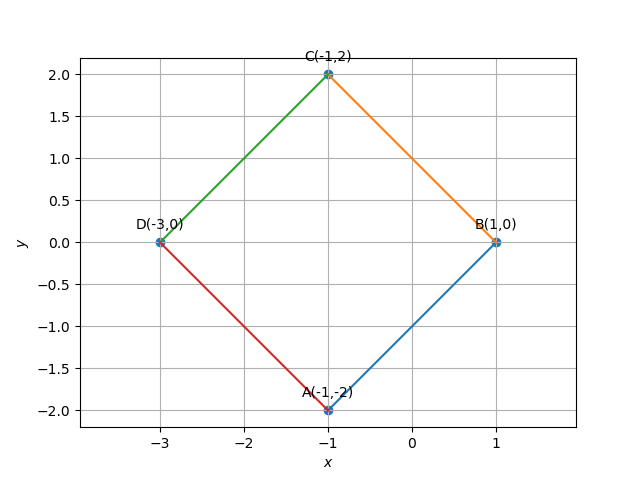
\includegraphics[width=0.75\columnwidth]{chapters/10/7/1/6/figs/quad1}
	\end{center}
\caption{}
\label{fig:10/7/1/6/Fig1}
\end{figure}
%
\begin{figure}[H]
	\begin{center} 
	    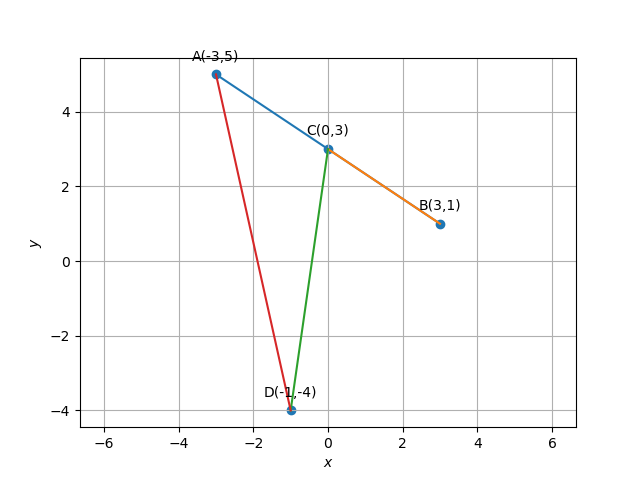
\includegraphics[width=0.75\columnwidth]{chapters/10/7/1/6/figs/quad2}
	\end{center}
\caption{}
\label{fig:10/7/1/6/Fig2}
\end{figure}
%	
\begin{figure}[H]
	\begin{center} 
	    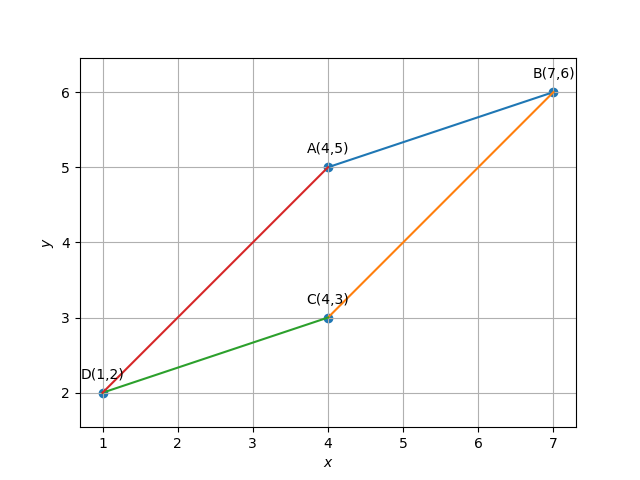
\includegraphics[width=0.75\columnwidth]{chapters/10/7/1/6/figs/quad3}
	\end{center}
\caption{}
\label{fig:10/7/1/6/Fig3}
\end{figure}
%
\begin{table}[H]
    \centering
%    \begin{tabular}{|c|c|c|c|c|}
	    \begin{tabularx}{\columnwidth}{|c|X|X|X|c|}
        \hline
		    &{\scriptsize $\vec{B}-\vec{A} = \vec{C}-\vec{D}$?} & {\tiny $(\vec{B}-\vec{A})^\top (\vec{C}-\vec{B}) =  0$?} & {\tiny $(\vec{C}-\vec{A})^\top (\vec{D}-\vec{B}) = 0$}& \textbf{Geometry}\\
        \hline
	    a)& Yes & Yes & Yes& Square \\
        \hline
	    b)& No & -&- & Triangle\\
        \hline
	    c)&Yes & No & No & Parallelogram\\
        \hline
	\end{tabularx}
%    \end{tabular}
	\caption{}
	\label{tab:10/7/1/6/inner}
\end{table}

\item Find the projection of the vector $\hat{i}+3\hat{j}+7\hat{k}$ on the vector $7\hat{i}-\hat{j}+8\hat{k}$.
	\\
	\solution
				Let 
\begin{align}
 \vec{A} =\myvec{1\\3\\7}, \vec{B} =\myvec{7\\-1\\8}
\end{align}
The projection of $\vec{A}$ on $\vec{B}$ is defined as
the foot of the perpendicular from 
$\vec{A}$ to $\vec{B}$ and obtained in 
	\eqref{eq:12/10/3/4/proj}.
Substituting numerical values,
\begin{align}
	\vec{C}
		=\frac{10}{19}\myvec{7\\-1\\8}
 \end{align}

\item Find the projection of the vector $\hat{i}-\hat{j}$ on the vector $\hat{i}+\hat{j}$.
	\\
\solution
		The given points are
\begin{align}
 \vec{A}=\myvec{1\\ -1},
 \vec{B}=\myvec{1\\ 1}
\end{align}
Since
\begin{align}
	\vec{A}^\top \vec{B} =0,
\end{align}
	from \eqref{eq:12/10/3/4/proj},
the projection vector is the origin.
		See \figref{fig:12/10/3/3fig}.
\begin{figure}[H]
	\centering
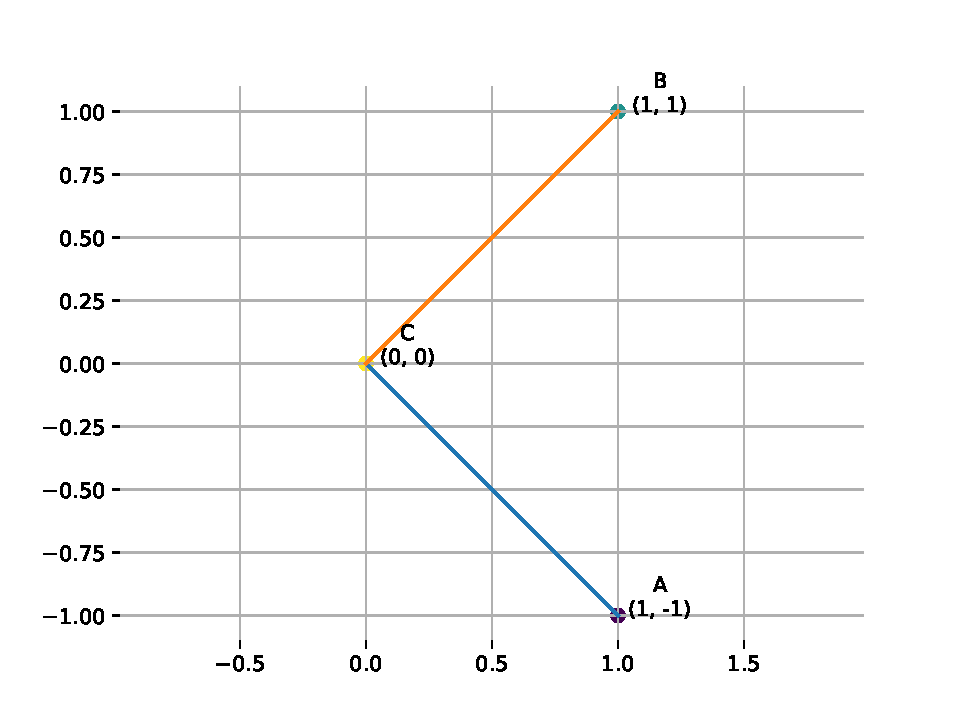
\includegraphics[width=0.75\columnwidth]{chapters/12/10/3/3/figs/fig.pdf}
\caption{}
		\label{fig:12/10/3/3fig}
\end{figure}

\item Show that each of the given three vectors is a unit vector: 
 $\frac{1}{7}(2\hat{i}+3\hat{j}+6\hat{k}),\frac{1}{7}(3\hat{i}-6\hat{j}+2\hat{k}),\frac{1}{7}(6\hat{i}+2\hat{j}-3\hat{k}$).
Also,show that they are mutually perpendicular to each other.
	\\
	\solution
		\begin{align}
\vec{A} = 	\myvec{
	\frac{2}{7} & \frac{3}{7} & \frac{6}{7} \\[1ex]
    \frac{3}{7} & -\frac{6}{7} & \frac{2}{7} \\[1ex]
    \frac{6}{7} & \frac{2}{7} & -\frac{3}{7}
}
\end{align}
is an orthogonal matrix satisfying
\eqref{eq:12/10/3/5/inner},
which verifies the given conditions.

\item If $\overrightarrow {a}=2\hat{i}+2\hat{j}3\hat{k},\overrightarrow {b}=\hat{-i}+2\hat{j}+\hat{k}$ and $\overrightarrow {c}=3\hat{i}+\hat{j}$ are such that $\overrightarrow {a}+\lambda\overrightarrow {b}$ is perpendicular to $\overrightarrow {c}$,then find the value of $\lambda$.
	\\
		\solution
\begin{align}
\because	(\vec{a}+\lambda \vec{b})^{\top} \vec{c} = 0,
	\\
	\lambda=-\frac{\vec{a}^{\top}\vec{c}}{\vec{b}^{\top}\vec{c}}
	=8,
\end{align}
upon substituting numerical values.



\item Show that $\abs {\overrightarrow {a}}\overrightarrow {b}+\abs{\overrightarrow {b}}\overrightarrow {a}$ is perpendicular to $\abs{\overrightarrow {a}} \overrightarrow {b}-\abs{\overrightarrow {b}} \overrightarrow {a}$, for any two nonzero vectors $\overrightarrow {a}$ and $\overrightarrow {b}$.
	\\
	\solution
		\begin{align}
\norm{\vec{a}}\vec{b}+\norm{\vec{b}}\vec{a}
=
	\norm{\vec{a}}\norm{\vec{b}}\brak{\frac{\vec{b}}{\norm{\vec{b}}}+\frac{\vec{a}}{\norm{\vec{a}}}}
	\\
\norm{\vec{a}}\vec{b}-\norm{\vec{b}}\vec{a}
=
	\norm{\vec{a}}\norm{\vec{b}}\brak{\frac{\vec{b}}{\norm{\vec{b}}}-\frac{\vec{a}}{\norm{\vec{a}}}}
	\\
	\implies 
	\brak{\norm{\vec{a}}\vec{b}+\norm{\vec{b}}\vec{a}}^{\top} \brak{\norm{\vec{a}}\vec{b}-\norm{\vec{b}}\vec{a}} = 0
\end{align}
	from \eqref{eq:12/10/3/11/unit}.

\item If $\overrightarrow {a},\overrightarrow {b},\overrightarrow {c}$ are unit vectors such that $\overrightarrow {a}+\overrightarrow {b}+\overrightarrow {c}=\overrightarrow {0}$, find the value of $\overrightarrow {a}.\overrightarrow {b}+\overrightarrow {b}.\overrightarrow {c}+\overrightarrow {c}.\overrightarrow {a}$.
	\\
	\solution
		\begin{align}
	\norm{{\vec{a}}+{\vec{b}}+{\vec{c}}}^2=0
	\nonumber \\
	\implies{\norm{\vec{a}}}^2+{\norm{\vec{b}}}^2+{\norm{\vec{c}}}^2+2({{\vec{a}^\top}{\vec{b}}+{\vec{b}^\top}{\vec{c}}+{\vec{c}^\top}{\vec{a}}})=0
	\nonumber \\
	\implies3+2({{\vec{a}^\top}{\vec{b}}+{\vec{b}^\top}{\vec{c}}+{\vec{c}^\top}{\vec{a}}})=0\nonumber \\
	\implies{\vec{a}^\top}{\vec{b}}+{\vec{b}^\top}{\vec{c}}+{\vec{c}^\top}\vec{a}=-\frac{3}{2}
\end{align}

\item If either vector $\overrightarrow {a}=0$ or $\overrightarrow {b}=0$, then $\overrightarrow {a}.\overrightarrow {b}$=0. But the converse need not be true. Justify your answer with an example.
	\\
	\solution
		\begin{align}
	\vec{a}=\myvec{1\\1},\,
\vec{b}=\myvec{1\\-1}\\
\implies \vec{a} ^\top \vec{b} =  0 
\end{align}



\item Show that the vectors $2\hat{i}-\hat{j}+\hat{k},\hat{i}-3\hat{j}-5\hat{k}$ and  $3\hat{i}-4\hat{j}-4\hat{k}$ from the vertices of a right angled triangle.
	\\
	\solution
		\begin{align}
\vec{A} = \myvec{2\\-1\\1}, \, \vec{B} = \myvec{1\\-3\\-5}, \, \vec{C}=\myvec{3\\-4\\-4},
\\
\implies \vec{B}-\vec{C} = \myvec{-2\\1\\-1} ,\, 
\vec{C}-\vec{A} = \myvec{1\\-3\\-5} ,\, 
\\
	\text{or, }
\brak{\vec{B}-\vec{C}}^{\top}\brak{\vec{C}-\vec{A}} = 0
\end{align}

\item Show that the points A, B and C with position vectors, $3\hat{i}-4\hat{j}-4\hat{k}, 2\hat{i}-\hat{j}+\hat{k}$ and $\hat{i}-3\hat{j}-5\hat{k}$, respectively, form the vertices of a right angled
triangle.
\\
\solution
		    \begin{align}
         \vec{B} - \vec{A} = \myvec{-1\\3\\5},\, 
         \vec{C} - \vec{B} = \myvec{-1\\-2\\-6},\,
         \vec{C} - \vec{A} = \myvec{-2\\1\\-1},
        \label{eq:chapters/12/10/2/17/dir-vec}
	\\
	    \implies 
	    \brak{\vec{B} - \vec{A}}^\top
	    \brak{\vec{C} - \vec{A}} = 0
    \end{align}
Hence, $\triangle ABC$ is right angled at $\vec{A}$. 

\item Let $\vec{a}=\hat{i}+4\hat{j}+2\hat{k}, \vec{b}=3\hat{i}-2\hat{j}+7\hat{k}$ and $\vec{c}=2\hat{i}-\hat{j}+4\hat{k}$. Find a vector $\vec{d}$ which is perpendicular to both $\vec{a}$ and $\vec{b}$, and $\vec{c}\cdot \vec{d}$=15.\\
	\solution
		From the given information, 
\begin{align}
\vec{a}^{\top}\vec{d} &= 0\\
\vec{b}^{\top}\vec{d} &= 0\\
\vec{c}^{\top}\vec{d} &= 15
\end{align}
yielding
\begin{align}
\myvec{\vec{a}^{\top} \\\vec{b}^{\top}\\\vec{c}^{\top}}\vec{d} &= \myvec{0\\0\\15}\\
\implies \myvec{1&4&2 \\3&-2&7 \\2&-1&4}\vec{d} &= \myvec{0\\0\\15}
\label{eq:chapters/12/10/5/12/1}
\end{align}
%
Forming the augmented matrix, 
\begin{align}
	\myvec{1&4&2&\vrule&0\\ 3&-2&7&\vrule&0 \\ 2&-1&4&\vrule&15} 
	\xleftrightarrow[R_3\leftarrow R_3-2R_1]{R_2\leftarrow R_2-3R_1}
	\myvec{1&4&2&\vrule&0\\ 0&-14&1&\vrule&0 \\ 0&-9&0&\vrule&15}
\nonumber	\\
	\xleftrightarrow[]{R_3\leftarrow R_3-\frac{9}{14}R_2}
	\myvec{1&4&2&\vrule&0\\ 0&-14&1&\vrule&0 \\ 0&0&-\frac{9}{14}&\vrule&15}
	\label{eq:chapters/12/10/5/12/2}
\end{align}
yielding
%
\begin{align}
	\vec{d} &= \myvec{\frac{160}{3}\\[1ex]-\frac{5}{3}\\[1ex]-\frac{70}{3}}
\end{align}
upon back substitution.


\item Prove that $(\vec{a}+\vec{b})\cdot(\vec{a}+\vec{b})=|{\vec{a}}|^2+|{\vec{b}}|^2$, if and only if $\vec{a}, \vec{b}$ are perpendicular, given $\vec{a}\neq\vec{0}, \vec{b}\neq\vec{0}$.\\
	\solution
			\begin{align}
\because 		\brak{\vec{a}+\vec{b}}^{\top}\brak{\vec{a}+\vec{b}} 
		= \norm{\vec{a}}^2+\norm{\vec{b}}^2,
		\\
		 \norm{\vec{a}}^2+\norm{\vec{b}}^2+2\vec{a}^{\top}\vec{b}
		= \norm{\vec{a}}^2+\norm{\vec{b}}^2
		\\
		\implies 
		\vec{a}^{\top}\vec{b} = 0 
	\end{align}


\item $ABCD$ is a rectangle formed by the points $\vec{A}(–1, –1), \vec{B}(– 1, 4), \vec{C}(5, 4)$  and  $\vec{D}(5, – 1)$. $\vec{P}, \vec{Q}, \vec{R}$ and $\vec{S}$ are the mid-points of $AB, BC, CD$ and $DA$ respectively. Is the quadrilateral $PQRS$ a square? a rectangle? or a rhombus? Justify your answer.
	\\
	\solution 
See Fig. \ref{fig:10/7/4/8Fig3}. From 
  \eqref{eq:10/7/4/8det2f}, $PQRS$ is a parallelogram.
\begin{align}
  %\label{eq:10/7/4/8det2f}
  \vec{P}  = 
 \frac{3}{2},\, 
 \vec{Q}  = \myvec{
 2 \\
 4 \\
 } ,\,
 \vec{R}  = \myvec{
 5 \\
 \frac{3}{2}
 }   
  ,\,
 \vec{S}  = \myvec{
 2\\
 -1 \\
 }   
 \\
	\implies 
 \brak{\vec{Q}-\vec{P}}^\top\brak{\vec{R}-\vec{Q}}  \neq 0
 \\
 \brak{\vec{R}-\vec{P}}^\top\brak{\vec{S}-\vec{Q}}  = 0
\end{align}
Therefore $PQRS$ is a rhombus.
\begin{figure}[!h]
	\begin{center}
		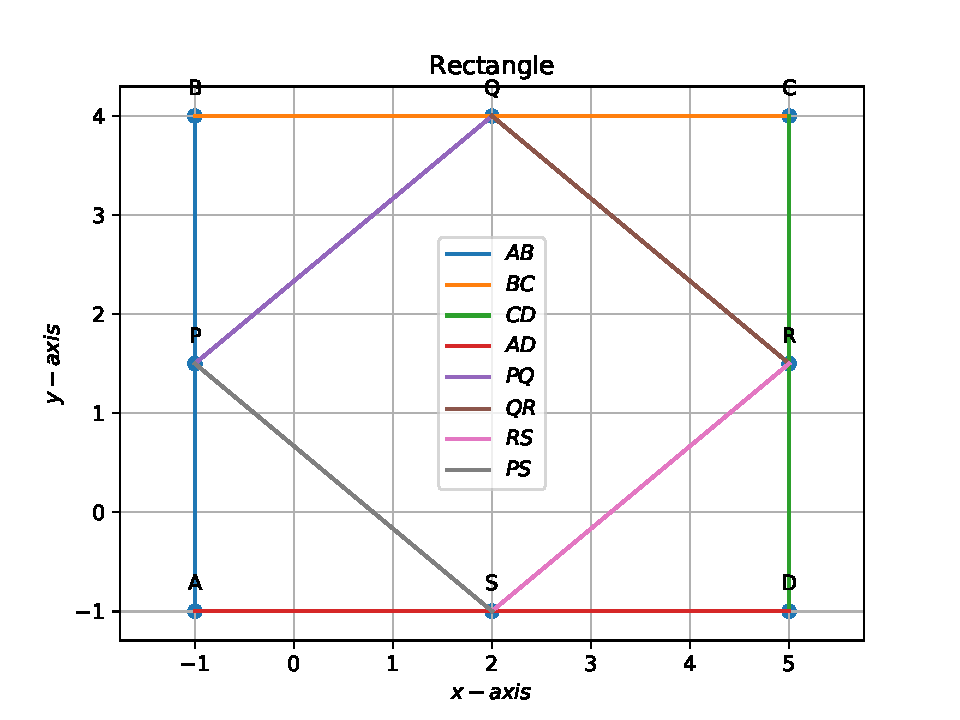
\includegraphics[width=\columnwidth]{chapters/10/7/4/8/figs/problem1.pdf}
	\end{center}
\caption{}
\label{fig:10/7/4/8Fig3}
\end{figure}


\item Without using the Baudhayana theorem, show that the points $A(4,4), B(3,5)$ and $C(-1,-1)$ are the vertices of a right angled triangle.
\label{chapters/11/10/1/6}
		See \figref{fig:11/10/1/6}.
\begin{align}
	\vec{C}-\vec{A}=\myvec{
-5 \\
	-5},\,
	\vec{A}-\vec{B}&=\myvec{
1 \\
-1 
}
\\
	\implies \brak{\vec{C}-\vec{A}}^{\top}
	\brak{\vec{A}-\vec{B}}&=0
\end{align}
Thus, $AB \perp AC$.
	\begin{figure}[H]
		\centering
 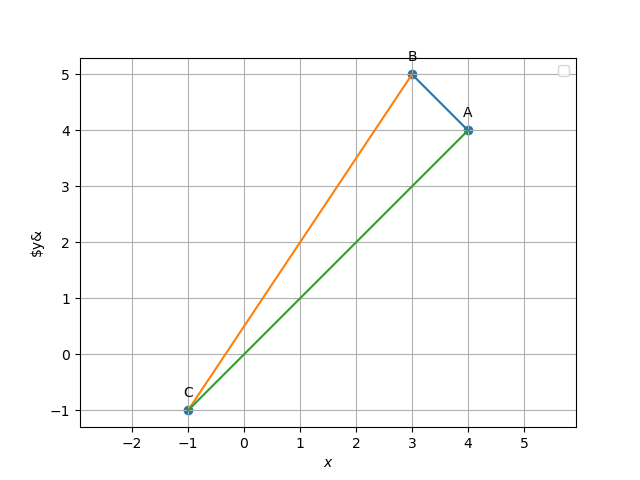
\includegraphics[width=0.75\columnwidth]{chapters/11/10/1/6/figs/triangle.png}
		\caption{}
		\label{fig:11/10/1/6}
  	\end{figure}

\item The line through the points $(h, 3)$ and $(4, 1)$ intersects the line $7x- 9y- 19= 0$ at a right angle. Find the value of $h$.
\label{chapters/11/10/3/10}
\\
\solution
The direction vectors of the given lines are 
\begin{align}
\myvec{4-h\\ -2}
,\,
\myvec{9\\ 7}
\\
\implies 
\myvec{9& 7}\myvec{4-h\\ -2}=0\\
\implies h=\frac{22}{9}
\end{align}
See  
		\figref{fig:chapters/11/10/3/10/Figure}.
\begin{figure}[h]
\centering
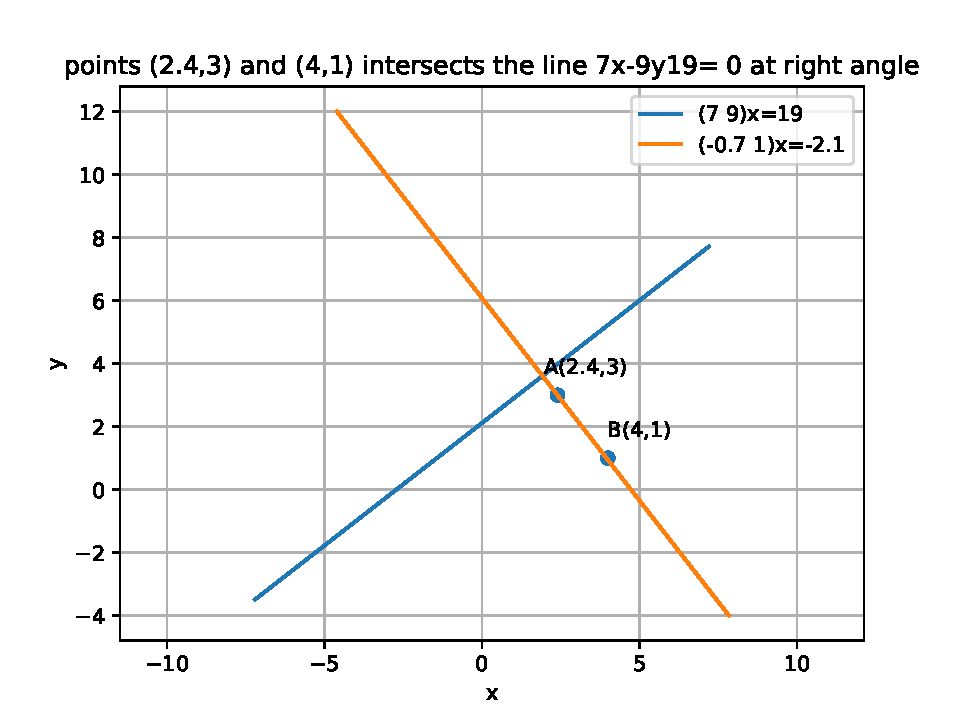
\includegraphics[width=\columnwidth]{chapters/11/10/3/10/figs/fig.pdf}
\caption{}
		\label{fig:chapters/11/10/3/10/Figure}
\end{figure}

\item In the following cases, determine whether the given planes are parallel or perpendicular, and in case they are neither, find the angles between them.
\begin{enumerate}
\item $7x + 5y + 6z + 30 = 0$ and $3x – y – 10z + 4 = 0$
\item $2x + y + 3z – 2 = 0$ and $x – 2y + 5 = 0$
\item $2x – 2y + 4z + 5 = 0$ and $3x – 3y + 6z – 1 = 0$
\item $2x – y + 3z – 1 = 0$ and $2x – y + 3z + 3 = 0$
\item $4x + 8y + z – 8 = 0$ and $y + z – 4 = 0$
\end{enumerate}
    \solution
		    See \tabref{tab:12/11/3/13}.
\begin{table}[htbp]
    \centering
    \caption{}
    \label{tab:12/11/3/13}
    \begin{tabular}{|c|c|c|c|c|c|}
        \hline
        $\vec{n}_1$ & $\vec{n}_1$ & $\vec{n}_1^{\top}\vec{n}_2$ & $\norm{\vec{n}_1}$ & $\norm{\vec{n}_2}$ & Angle\\
        \hline
        $\myvec{7\\5\\6}$ & $\myvec{3\\-1\\-10}$ & $-44$ & $\sqrt{110}$ & $\sqrt{110}$ & $\cos^{-1}-\frac{2}{5}$ \\
        \hline
        $\myvec{2\\1\\3}$ & $\myvec{1\\-2\\0}$ & $0$ & & & perpendicular \\
        \hline
        $\myvec{2\\-2\\4}$ & $\myvec{3\\-3\\6}$ & $36$ & $\sqrt{24}$ & $\sqrt{54}$ & parallel \\
        \hline
        $\myvec{2\\-1\\3}$ & $\myvec{2\\-1\\3}$ & $14$ & $\sqrt{14}$ & $\sqrt{14}$ & parallel \\
        \hline
        $\myvec{4\\8\\1}$ & $\myvec{0\\1\\1}$ & $9$ & $9$ & $\sqrt{2}$ & $45\degree$ \\
        \hline
    \end{tabular}
\end{table}

\iffalse
\begin{table}[htbp]
    \centering
    \caption{}
    \label{}
    \begin{tabular}{|c|c|c|c|c|c|}
        \hline
	    $\vec{n}_1$ & $\vec{n}_1$ &  $\vec{n}_1^{\top}\vec{n}_2$& $\norm{\vec{n}_1}$ &$\norm{\vec{n}_2}$  &  Angle\\
        \hline
	    \myvec{7\\5\\6} & \myvec{3\\-1\\-10} & -44 & \sqrt{110} &\sqrt{110}  & \cos^{-1}-\frac{2}{5} \\
        \hline
\myvec{2\\1\\3}  & \myvec{1\\-2\\0}& 0 &  &  & perpendicular\\
        \hline
 \myvec{2\\-2\\4} & \myvec{3\\-3\\6} & 36  & \sqrt{24} & \sqrt{54} &  parallel \\
        \hline
 \myvec{2\\-1\\3} & \myvec{2\\-1\\3} & 14 & \sqrt{14} & \sqrt{14} & parallel \\
        \hline
 \myvec{4\\8\\1} & \myvec{0\\1\\1} & 9 & 9 & \sqrt{2} &  45\degree  \\
        \hline
    \end{tabular}
\end{table}
\fi

		\item 
 Show that the line joining the origin to the point $P(2, 1, 1)$ is perpendicular to the
line determined by the points $A(3, 5, – 1), B(4, 3, – 1)$.
\\
    \solution
				\begin{align}
			\brak{\vec{A}-\vec{B}}^\top\vec{P}=
			\myvec{-1&2&0}\myvec{2\\1\\1}=0 \qed
		\end{align}

	\item  If $l_1, m_1,n_1 \text{ and } l_2,m_2,n_2$ are the direction cosines of two mutually perpendicular lines, show that the direction cosines of the line perpendicular to both these are  $m_1n_2-m_2n_1,n_1l_2-n_2l_1,l_1m_2-l_2m_1$.
\\
    \solution
		\begin{align}
\vec{P} 
	=\myvec{
l_1&l_2&m_1n_2-m_2n_1\\
        m_1&m_2&n_1l_2-n_2l_1\\
        n_1&n_2&l_1m_2-l_2m_1
}
	\end{align}
	satisfies 
\eqref{eq:12/10/3/5/inner}.
	Hence, the three vectors are mutually perpendicular.

	\item If the lines $\frac{x-1}{-3} = \frac{y-2}{2k} = \frac{z-3}{2}$ and  $\frac{x-1}{3k} = \frac{y-1}{1} = \frac{z-6}{-5}$ are perpendicular, find the value of $k$.\\
    \solution
		From the given information,
\begin{align}
\vec{m}_1 = \myvec{-3\\ 2k\\ 2},\,  \vec{m}_2 =\myvec{3k\\ 1\\ -5} 
\\
	\implies \myvec{-3& 2k& 2}^{\top} \myvec{3k\\ 1\\ -5} =0
	\\
	\implies k = -\frac{10}{7}
\end{align}
See 
     \figref{fig:chapters/12/11/4/6/1}
\begin{figure}[h!]
  \centering
   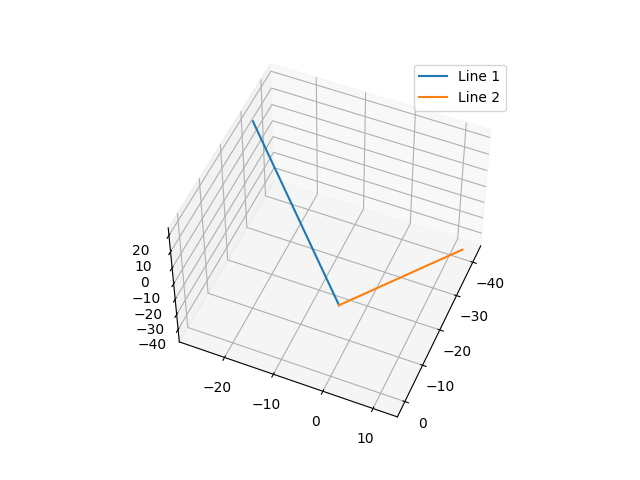
\includegraphics[width=\columnwidth]{chapters/12/11/4/6/figs/line_1.png}
    \caption{lines represented for the given points and direction vector with k=$\frac{-10}{7}$}
     \label{fig:chapters/12/11/4/6/1}
     \end{figure}  



\item If $\vec{a},\vec{b},\vec{c}$ are mutually perpendicular vectors of equal magnitudes, show that the vector $\vec{c}\cdot\vec{d}$=15 is equally inclined to $\vec{a},\vec{b}$ and $\vec{c}$.
    \item If $ \vec{A},\vec{B},\vec{C} $ are mutually perpendicular vectors of equal magnitudes,show that the  $ \vec{A}+\vec{B}+\vec{C} $ is equally inclined to $ \vec{A},\vec{B}  \text{ and }  \vec{C} $.
\item Check whether $(5,-2), (6,4)$ and $(7,-2)$ are the vertices of an isosceles triangle.
\item The perpendicular bisector of the line segment joining the points $\vec{A} (1, 5) \text{ and }
\vec{B} (4, 6)$ cuts the y-axis at
\begin{enumerate}
	\item$(0, 13)$ 
	\item $(0, –13)$
	\item$(0, 12) $
	\item$(13, 0)$
\end{enumerate}
\item The point which lies on the perpendicular bisector of the line segment joining the
	points $\vec{A} (–2, –5)\text { and } \vec{B} (2, 5) $ is
\begin{enumerate}
\item  	$(0, 0)$
\item  $(0, 2)$ 
\item  $(2, 0)$ 
\item  $(–2, 0)$
\end{enumerate}
\item The points $ (–4, 0), (4, 0), (0, 3) $ are the vertices of
	\begin{enumerate}
\item right triangle 
\item isosceles triangle
\item  equilateral triangle
\item  scalene triangle 
\end{enumerate}
\item The point $\vec{A}(2,7)$ lies on the perpendicular bisector of line segment joining the points $\vec{P}(6,5)\text{ and } \vec{Q}(0,-4)$.
\item The points $\vec{A}(-1,-2), \vec{B}(4,3), \vec{C}(2,5) \text{ and } \vec{D}(-3,0)$ in that order form a rectangle.
\item Name the type of triangle formed by the points $\vec{A}(-5,6),\vec{B}(-4,-2),\text{ and }\vec{C}(7,5)$.
\item What type of a quadrilateral do the points $\vec{A}(2,-2),\vec{B}(7,3),\vec{C}(11,-1),\text{ and }\vec{D}(6,-6)$ taken in that order, form?
\item Find the coordinates of the point $\vec{Q}$ on the $x$-axis which lies on the perpendicular bisector of the line segment joining the points $\vec{A}(-5,-2) \text{ and } \vec{B}(4,-2)$. Name the type of triangle formed by points $\vec{Q},\vec{A}\text{ and }\vec{B}$.
\item The points $\vec{A}(2,9),\vec{B}(a,5) \text{ and }\vec{C}(5,5)$ are the vertices of a triangle $\vec{ABC}$ right angled at $\vec{B}$. Find the values of a and hence the area of $\triangle \vec{ABC}$.
\item Find a vector of magnitude 6, which is perpendicular to both the vectors $2\hat{i}-\hat{j}$+$2\hat{k}\text{ and }4\hat{i}-\hat{j}+3\hat{k}$.
\item If A,B,C,D  are the points with position vectors $\hat{i}+\hat{j}-\hat{k}$, $2\hat{i}-\hat{j}+3\hat{k}$, $2\hat{i}-3\hat{k}$, $3\hat{i}$-$2\hat{j}$+$\hat{k}$, respectively, find the projection of $\overline{AB}$ $\text{ along }$ $\overline{CD}$.
\item Find the value of $\lambda$ such that the vectors $\vec{a}=2\hat{i}+\lambda\hat{j}+\hat{k}$ $\text{and}$ $\vec{b}=\hat{i}+2\hat{j}+3\hat{k}$ are orthogonal.
	\begin{enumerate}
\item 0
\item 1 
\item $\frac{3}{2}$
\item $-\frac{5}{2}$
	\end{enumerate}
\item Projection vector of $\vec{a}$ on $\vec{b}$ is
	\begin{enumerate}
\item $\left(\dfrac{\vec{a}\cdot\vec{b}}{\abs{\vec{b}}^2}\right)$
\item $\frac{\vec{a}\cdot\vec{b}}{\abs{\vec{b}}}$
\item $\frac{\vec{a}\cdot\vec{b}}{\abs{\vec{a}}}$
\item $\left(\dfrac{\vec{a}\cdot\vec{b}}{\abs{\vec{a}}^2}\right)$
\end{enumerate}
\item The vectors $\lambda\hat{i}+\lambda\hat{j}+2\hat{k}$, $\hat{i}+\lambda\hat{j}-\hat{k}$ $\text{ and }$ $2\hat{i}-\hat{j}+\lambda\hat{k}$ are coplanar if
	\begin{enumerate}
\item	$\lambda=-2$
\item $\lambda=0$
\item $\lambda=1$
\item	$\lambda=-1$
\end{enumerate}
\item The number of vectors of unit length perpendicular to the vectors $\vec{a}=2\hat{i}+\hat{j}+2\hat{k}$ $\text{ and }$ $\vec{b}=\hat{j}+\hat{k}$ is
	\begin{enumerate}
\item one
\item  two
\item three
\item infinite
\end{enumerate}
\item If $\vec{r}\cdot\vec{a}=0, \vec{r}\cdot\vec{b}=0$ and $\vec{r}\cdot\vec{c}=0$ for some non-zero vector $\vec{r}$, then the value of $\vec{a}\cdot(\vec{b}\times\vec{c})$ is \rule{1cm}{0.15mm}.
\item If $\abs{\vec{a}+\vec{b}}$ = $\abs{\vec{a}-\vec{b}}$, then the vectors $\vec{a}$ $\text {and}$ $\vec{b}$ are orthogonal.
\item Prove that the lines $x=py+q , z=ry+s \text{ and } x=p^{\prime}y+q^{\prime}, z=r^{\prime}y+s^{\prime} $ are perpendicular if $pp^{\prime}+rr^{\prime}+1=0$.
\item Find the equation of a plane which  bisects perpendicularly the line joining the points A$(2,3,4)$ and B$(4,5,8)$ at right angles.
\item $\overrightarrow{AB}=3\hat{i}-\hat{j}+\hat{k}$ and $\overrightarrow{CD}=-3\hat{i}+2\hat{j}+4\hat{k}$ are two vectors. The position vectors of the points A and C are $6\hat{i}+7\hat{j}+4\hat{k}$ and $-9\hat{j}+2\hat{k},$ respectively. Find the position vector of a point P on the line AB and a point Q on the line CD such that $\overrightarrow{PQ}$ is perpendicular to $\overrightarrow{AB}$ and $\overrightarrow{CD}$ both.
\item Show that the straight lines whose direction cosines are given by $2l+2m-n=0$ and $mn+nl+lm=0$ are at right angles.
\item If $l_1, m_1, n_1;l_2, m_2, n_2;l_3, m_3, n_3$ are the direction cosines of the three mutually perpendcular lines, prove that the line whose direction cosines are propotional to $l_1+l_2+l_3 , m_1+m_2,m_3, n_1+n_2+n_3$ make angles with them.
\item The intercepts made by the plane $2x-3y+5z+4=0$ on the co-ordinate axis are $\brak{-2,\dfrac{4}{3},-\dfrac{4}{5}}$.
\item The line $\overrightarrow{r}=2\hat{i}-3\hat{j}-\hat{k}+\lambda(\hat{i}-\hat{j}+2\hat{k})$ lies in the plane $\overrightarrow{r} \cdot (3\hat{i}+\hat{j}-\hat{k})+2=0$.
\end{enumerate}

\newpage
\subsection{Vector Product}
\begin{enumerate}[label=\thesection.\arabic*,ref=\thesection.\theenumi]
		\item Find $\abs{\overrightarrow{a}\times\overrightarrow{b}},\text{ if }\overrightarrow{a}=\hat{i}-7\hat{j}+7\hat{k}\text{ and } \overrightarrow{b}=3\hat{i}-2\hat{j}+2\hat{k}$.
	\\
		\solution
		\iffalse
\documentclass[12pt]{article}
\usepackage{graphicx}
\usepackage[none]{hyphenat}
\usepackage{listings}
\usepackage[english]{babel}
\usepackage{booktabs}
\usepackage{caption}
\usepackage{booktabs}
\usepackage{array}
\usepackage{commath}
\usepackage{amssymb}
\usepackage{amsmath}
%\usepackage{extarrows}
\usepackage{commath}
%\usepackage[utf8]{inputenc}
\lstset{ language=tex,
	frame=single,
         breaklines=true
        }
        \usepackage{hyper ref}
        \usepackage{atbegshi}
        \AtBeginDocument{\AtBeginShipoutNext{\AtBeginShipoutDiscard}}

        \newcommand{\mydet}[1]{\ensuremath{\begin{vmatrix}#1\end{vmatrix}}}
        \providecommand{\abs}[1]{\left\vert#1\right\vert}
        \providecommand{\brak}[1]{\ensuremath{\left(#1\right)}}
\providecommand{\norm}[1]{\left\lVert#1\right\rVert}
\newcommand{\solution}{\noindent \textbf{Solution: }}
\newcommand{\myvec}[1]{\ensuremath{\begin{pmatrix}#1\end{pmatrix}}}
\let\vec\mathbf

\begin{document}
\begin{center}\title{\textbf{Vectors Assignment-1}}
	\date{\vspace{-5ex}}
\maketitle
\end{center}
\setcounter{page}{1}
Section{12${th}$Math- Excercise 12.10.4.1}

\begin{enumerate}
	\item Find $\abs{\vec{a}\times\vec{b}}$, if $\vec{a}=\hat{i}-7\hat{j}+7\hat{k}$ $\text{ and } $ $\vec{b}=3\hat{i}-2\hat{j}+2\hat{k}$

\solution
\fi
Since 
\begin{align}
	\mydet{\vec{A}_{23}&\vec{B}_{23}}&=\mydet{-7 & -2 \\ 7 & 2}=-14+14=0\\
	\mydet{\vec{A}_{31}&\vec{B}_{31}}&=\mydet{1 & 3 \\ 7 & 2}=2-21=-19\\
	\mydet{\vec{A}_{12}&\vec{B}_{12}}&=\mydet{1 & 3 \\ -7 & -2}=-2+21=19,
	\\
	\norm{\vec{a}\times\vec{b}}&=\brak{\mydet{\vec{A}_{23}& \vec{B}_{23} \\ \vec{A}_{31} & \vec{B}_{31} \\ \vec{A}_{12}& \vec{B}_{12}}}
=19\sqrt{2}
\end{align}

\item Find $\lambda$ and $\mu$ if $(2\hat{i}+6\hat{j}+27\hat{k})\times(\hat{i}+\lambda \hat{j} + \mu \hat{k})=\overrightarrow{0}$.
	\\
		\solution
		From 
		 Formula \ref{prop:lin-dep-cross},
performing row reduction, 
\begin{align}
 \myvec{2&6&27 \\ 1& \lambda & \mu}
	\xleftrightarrow{R_{2}\leftarrow 2R_{2}-R_{1}}  	
 \myvec{2&6&27 \\ 0& 2\lambda -6 & 2\mu-27}
\end{align}
For the above matrix to have rank 1,
\begin{align}
	\mu=\frac{27}{2},
	\lambda=3.
\end{align}


\item Find the area of the triangle with vertices $A(1, 1, 2), B(2, 3, 5)$ and $C(1, 5, 5)$.
	\\
		\solution
		\iffalse
\documentclass[journal,12pt,twocolumn]{IEEEtran}
\usepackage{setspace}
\usepackage{gensymb}
\singlespacing
\usepackage[cmex10]{amsmath}
\usepackage{amsthm}
\usepackage{mathrsfs}
\usepackage{txfonts}
\usepackage{stfloats}
\usepackage{bm}
\usepackage{cite}
\usepackage{cases}
\usepackage{subfig}
\usepackage{longtable}
\usepackage{multirow}
\usepackage{enumitem}
\usepackage{mathtools}
\usepackage{steinmetz}
\usepackage{tikz}
\usepackage{circuitikz}
\usepackage{verbatim}
\usepackage{tfrupee}
\usepackage[breaklinks=true]{hyperref}
\usepackage{tkz-euclide}
\usetikzlibrary{calc,math}
\usepackage{listings}
    \usepackage{color}                                            %%
    \usepackage{array}                                            %%
    \usepackage{longtable}                                        %%
    \usepackage{calc}                                             %%
    \usepackage{multirow}                                         %%
    \usepackage{hhline}                                           %%
    \usepackage{ifthen}                                           %%
  %optionally (for landscape tables embedded in another document): %%
    \usepackage{lscape}     
\usepackage{multicol}
\usepackage{chngcntr}
\DeclareMathOperator*{\Res}{Res}
\renewcommand\thesection{\arabic{section}}
\renewcommand\thesubsection{\thesection.\arabic{subsection}}
\renewcommand\thesubsubsection{\thesubsection.\arabic{subsubsection}}

\renewcommand\thesectiondis{\arabic{section}}
\renewcommand\thesubsectiondis{\thesectiondis.\arabic{subsection}}
\renewcommand\thesubsubsectiondis{\thesubsectiondis.\arabic{subsubsection}}

% correct bad hyphenation here
\hyphenation{op-tical net-works semi-conduc-tor}
\def\inputGnumericTable{}                                 %%

\lstset{
frame=single, 
breaklines=true,
columns=fullflexible
}

\begin{document}


\newtheorem{theorem}{Theorem}[section]
\newtheorem{problem}{Problem}
\newtheorem{proposition}{Proposition}[section]
\newtheorem{lemma}{Lemma}[section]
\newtheorem{corollary}[theorem]{Corollary}
\newtheorem{example}{Example}[section]
\newtheorem{definition}[problem]{Definition}
\newcommand{\BEQA}{\begin{eqnarray}}
\newcommand{\EEQA}{\end{eqnarray}}
\newcommand{\define}{\stackrel{\triangle}{=}}

\bibliographystyle{IEEEtran}
\providecommand{\mbf}{\mathbf}
\providecommand{\pr}[1]{\ensuremath{\Pr\left(#1\right)}}
\providecommand{\qfunc}[1]{\ensuremath{Q\left(#1\right)}}
\providecommand{\sbrak}[1]{\ensuremath{{}\left[#1\right]}}
\providecommand{\lsbrak}[1]{\ensuremath{{}\left[#1\right.}}
\providecommand{\rsbrak}[1]{\ensuremath{{}\left.#1\right]}}
\providecommand{\brak}[1]{\ensuremath{\left(#1\right)}}
\providecommand{\lbrak}[1]{\ensuremath{\left(#1\right.}}
\providecommand{\rbrak}[1]{\ensuremath{\left.#1\right)}}
\providecommand{\cbrak}[1]{\ensuremath{\left\{#1\right\}}}
\providecommand{\lcbrak}[1]{\ensuremath{\left\{#1\right.}}
\providecommand{\rcbrak}[1]{\ensuremath{\left.#1\right\}}}
\theoremstyle{remark}
\newtheorem{rem}{Remark}
\newcommand{\sgn}{\mathop{\mathrm{sgn}}}
\providecommand{\abs}[1]{\left\vert#1\right\vert}
\providecommand{\res}[1]{\Res\displaylimits_{#1}} 
\providecommand{\norm}[1]{\left\lVert#1\right\rVert}
\providecommand{\mtx}[1]{\mathbf{#1}}
\providecommand{\mean}[1]{E\left[ #1 \right]}
\providecommand{\fourier}{\overset{\mathcal{F}}{ \rightleftharpoons}}
\providecommand{\system}{\overset{\mathcal{H}}{ \longleftrightarrow}}
\newcommand{\solution}{\noindent \textbf{Solution: }}
\newcommand{\cosec}{\,\text{cosec}\,}
\providecommand{\dec}[2]{\ensuremath{\overset{#1}{\underset{#2}{\gtrless}}}}
\newcommand{\myvec}[1]{\ensuremath{\begin{pmatrix}#1\end{pmatrix}}}
\newcommand{\mydet}[1]{\ensuremath{\begin{vmatrix}#1\end{vmatrix}}}
\numberwithin{equation}{subsection}
\makeatletter
\@addtoreset{figure}{problem}
\makeatother

\let\StandardTheFigure\thefigure
\let\vec\mathbf
\renewcommand{\thefigure}{\theproblem}



\def\putbox#1#2#3{\makebox[0in][l]{\makebox[#1][l]{}\raisebox{\baselineskip}[0in][0in]{\raisebox{#2}[0in][0in]{#3}}}}
     \def\rightbox#1{\makebox[0in][r]{#1}}
     \def\centbox#1{\makebox[0in]{#1}}
     \def\topbox#1{\raisebox{-\baselineskip}[0in][0in]{#1}}
     \def\midbox#1{\raisebox{-0.5\baselineskip}[0in][0in]{#1}}

\vspace{3cm}


\title{Assignment 1}
\author{Jaswanth Chowdary Madala}





% make the title area
\maketitle

\newpage

%\tableofcontents

\bigskip

\renewcommand{\thefigure}{\theenumi}
\renewcommand{\thetable}{\theenumi}

\begin{enumerate}
\item Find the area of the triangle with vertices $\vec{A}$(1,1,2), $\vec{B}$ (2,3,5), $\vec{C}$ (1,5,5).

\textbf{Solution:} The area of the triangle $ABC$ is given by
\begin{align}
ar(ABC) &= \dfrac{1}{2}\norm{\brak{\vec{B}-\vec{A}} \times \brak{\vec{C}-\vec{A}}}
\end{align}


given points are 
\fi
Since
\begin{align}
\vec{B}-\vec{A} = \myvec{1\\2\\3}, 
\vec{C}-\vec{A} = \myvec{0\\4\\3} \\
\end{align}
the desired area is given by 
\begin{align}
	\frac{1}{2} \norm{\myvec{1\\2\\3} \times \myvec{0\\4\\3}} 
	= 	\frac{1}{2}\norm{\myvec{-6\\3\\4}}
= \dfrac{\sqrt{61}}{2}
\end{align}






\item Find the area of the parallelogram whose adjacent sides are determined by the vectors $\overrightarrow{a}=\hat{i}-\hat{j}+3\hat{k}$ and $\overrightarrow{b}=2\hat{i}-7\hat{j}+\hat{k}$.
	\\
		\solution
					From \eqref{eq:tri-area-cross},
			the desired area is obtained as
\begin{align}
	\norm{\myvec{1\\-1\\3} \times \myvec{2\\ -7 \\ 1}}
	=\norm{\myvec{20\\5\\-5}}
= 15\sqrt{2}
\end{align}


\item Let the vectors $\overrightarrow{a}$ and $\overrightarrow{b}$ be such that $|\overrightarrow{a}| = 3$ and $|\overrightarrow{b}| = \dfrac{\sqrt{2}}{3}$, then $\overrightarrow{a} \times \overrightarrow{b}$ is a unit vector, if the angle between $\overrightarrow{a}$ and $\overrightarrow{b}$ is
\begin{enumerate}
\item $\frac{\pi}{6}$
\item $\frac{\pi}{4}$
\item $\frac{\pi}{3}$
\item $\frac{\pi}{2}$
\end{enumerate}
		\solution
		From the given information and 
	\eqref{eq:cross-sin}
%
\begin{align}
	\norm{\vec{a} \times \vec{b}} & = \norm{\vec{a}} \norm{\vec{b}} \sin \theta =1\\
\implies\sin \theta & = \frac{1} {\norm{\vec{a}} \norm{\vec{b}}}
 = \frac{1}{\sqrt{2}}\\
\implies\theta &= 
 \frac{\pi}{4} 
\end{align}

\item Area of a rectangle having vertices A, B, C and D with position vectors $ -\hat{i}+ \frac{1}{2} \hat{j}+4\hat{k}, \hat{i}+ \frac{1}{2} \hat{j}+4\hat{k}, \hat{i}-\frac{1}{2} \hat{j}+4\hat{k}$ and $-\hat{i}- \frac{1}{2} \hat{j}+4\hat{k}$, respectively is
\begin{enumerate}
\item $\frac{1}{2}$
\item 1
\item 2
\item 4
\end{enumerate}
		\solution
		\iffalse
\documentclass[journal,12pt,twocolumn]{IEEEtran}
%
\usepackage{setspace}
\usepackage{gensymb}
%\doublespacing
\singlespacing

%\usepackage{graphicx}
%\usepackage{amssymb}
%\usepackage{relsize}
\usepackage[cmex10]{amsmath}
%\usepackage{amsthm}
%\interdisplaylinepenalty=2500
%\savesymbol{iint}
%\usepackage{txfonts}
%\restoresymbol{TXF}{iint}
%\usepackage{wasysym}
\usepackage{amsthm}
%\usepackage{iithtlc}
\usepackage{mathrsfs}
\usepackage{txfonts}
\usepackage{stfloats}
\usepackage{bm}
\usepackage{cite}
\usepackage{cases}
\usepackage{subfig}
%\usepackage{xtab}
\usepackage{longtable}
\usepackage{multirow}
%\usepackage{algorithm}
%\usepackage{algpseudocode}
\usepackage{enumitem}
\usepackage{mathtools}
\usepackage{steinmetz}
\usepackage{tikz}
\usepackage{circuitikz}
\usepackage{verbatim}
\usepackage{tfrupee}
\usepackage[breaklinks=true]{hyperref}
%\usepackage{stmaryrd}
\usepackage{tkz-euclide} % loads  TikZ and tkz-base
%\usetkzobj{all}
\usetikzlibrary{calc,math}
\usepackage{listings}
    \usepackage{color}                                            %%
    \usepackage{array}                                            %%
    \usepackage{longtable}                                        %%
    \usepackage{calc}                                             %%
    \usepackage{multirow}                                         %%
    \usepackage{hhline}                                           %%
    \usepackage{ifthen}                                           %%
  %optionally (for landscape tables embedded in another document): %%
    \usepackage{lscape}     
\usepackage{multicol}
\usepackage{chngcntr}
%\usepackage{enumerate}

%\usepackage{wasysym}
%\newcounter{MYtempeqncnt}
\DeclareMathOperator*{\Res}{Res}
%\renewcommand{\baselinestretch}{2}
\renewcommand\thesection{\arabic{section}}
\renewcommand\thesubsection{\thesection.\arabic{subsection}}
\renewcommand\thesubsubsection{\thesubsection.\arabic{subsubsection}}

\renewcommand\thesectiondis{\arabic{section}}
\renewcommand\thesubsectiondis{\thesectiondis.\arabic{subsection}}
\renewcommand\thesubsubsectiondis{\thesubsectiondis.\arabic{subsubsection}}

% correct bad hyphenation here
\hyphenation{op-tical net-works semi-conduc-tor}
\def\inputGnumericTable{}                                 %%

\lstset{
%language=C,
frame=single, 
breaklines=true,
columns=fullflexible
}
%\lstset{
%language=tex,
%frame=single, 
%breaklines=true
%}

\begin{document}
%


\newtheorem{theorem}{Theorem}[section]
\newtheorem{problem}{Problem}
\newtheorem{proposition}{Proposition}[section]
\newtheorem{lemma}{Lemma}[section]
\newtheorem{corollary}[theorem]{Corollary}
\newtheorem{example}{Example}[section]
\newtheorem{definition}[problem]{Definition}
%\newtheorem{thm}{Theorem}[section] 
%\newtheorem{defn}[thm]{Definition}
%\newtheorem{algorithm}{Algorithm}[section]
%\newtheorem{cor}{Corollary}
\newcommand{\BEQA}{\begin{eqnarray}}
\newcommand{\EEQA}{\end{eqnarray}}
\newcommand{\define}{\stackrel{\triangle}{=}}

\bibliographystyle{IEEEtran}
%\bibliographystyle{ieeetr}


\providecommand{\mbf}{\mathbf}
\providecommand{\pr}[1]{\ensuremath{\Pr\left(#1\right)}}
\providecommand{\qfunc}[1]{\ensuremath{Q\left(#1\right)}}
\providecommand{\sbrak}[1]{\ensuremath{{}\left[#1\right]}}
\providecommand{\lsbrak}[1]{\ensuremath{{}\left[#1\right.}}
\providecommand{\rsbrak}[1]{\ensuremath{{}\left.#1\right]}}
\providecommand{\brak}[1]{\ensuremath{\left(#1\right)}}
\providecommand{\lbrak}[1]{\ensuremath{\left(#1\right.}}
\providecommand{\rbrak}[1]{\ensuremath{\left.#1\right)}}
\providecommand{\cbrak}[1]{\ensuremath{\left\{#1\right\}}}
\providecommand{\lcbrak}[1]{\ensuremath{\left\{#1\right.}}
\providecommand{\rcbrak}[1]{\ensuremath{\left.#1\right\}}}
\theoremstyle{remark}
\newtheorem{rem}{Remark}
\newcommand{\sgn}{\mathop{\mathrm{sgn}}}
\providecommand{\abs}[1]{\left\vert#1\right\vert}
\providecommand{\res}[1]{\Res\displaylimits_{#1}} 
\providecommand{\norm}[1]{\left\lVert#1\right\rVert}
%\providecommand{\norm}[1]{\lVert#1\rVert}
\providecommand{\mtx}[1]{\mathbf{#1}}
\providecommand{\mean}[1]{E\left[ #1 \right]}
\providecommand{\fourier}{\overset{\mathcal{F}}{ \rightleftharpoons}}
%\providecommand{\hilbert}{\overset{\mathcal{H}}{ \rightleftharpoons}}
\providecommand{\system}{\overset{\mathcal{H}}{ \longleftrightarrow}}
	%\newcommand{\solution}[2]{\textbf{Solution:}{#1}}
\newcommand{\solution}{\noindent \textbf{Solution: }}
\newcommand{\cosec}{\,\text{cosec}\,}
\providecommand{\dec}[2]{\ensuremath{\overset{#1}{\underset{#2}{\gtrless}}}}
\newcommand{\myvec}[1]{\ensuremath{\begin{pmatrix}#1\end{pmatrix}}}
\newcommand{\mydet}[1]{\ensuremath{\begin{vmatrix}#1\end{vmatrix}}}
%\numberwithin{equation}{section}
\numberwithin{equation}{subsection}
%\numberwithin{problem}{section}
%\numberwithin{definition}{section}
\makeatletter
\@addtoreset{figure}{problem}
\makeatother

\let\StandardTheFigure\thefigure
\let\vec\mathbf
%\renewcommand{\thefigure}{\theproblem.\arabic{figure}}
\renewcommand{\thefigure}{\theproblem}
%\setlist[enumerate,1]{before=\renewcommand\theequation{\theenumi.\arabic{equation}}
%\counterwithin{equation}{enumi}


%\renewcommand{\theequation}{\arabic{subsection}.\arabic{equation}}

\def\putbox#1#2#3{\makebox[0in][l]{\makebox[#1][l]{}\raisebox{\baselineskip}[0in][0in]{\raisebox{#2}[0in][0in]{#3}}}}
     \def\rightbox#1{\makebox[0in][r]{#1}}
     \def\centbox#1{\makebox[0in]{#1}}
     \def\topbox#1{\raisebox{-\baselineskip}[0in][0in]{#1}}
     \def\midbox#1{\raisebox{-0.5\baselineskip}[0in][0in]{#1}}

\vspace{3cm}


\title{Question: 12.10.4.12}
\author{Nikam Pratik Balasaheb (EE21BTECH11037)}





% make the title area
\maketitle

\newpage

%\tableofcontents

\bigskip

\renewcommand{\thefigure}{\theenumi}
\renewcommand{\thetable}{\theenumi}
%\renewcommand{\theequation}{\theenumi}

\section{Problem}
Find the area of rectangle having A,B,C,D with position vectors $\myvec{-1\\[1pt]\frac{1}{2} \\[1pt] 4}$ ,$\myvec{1\\[1pt]\frac{1}{2} \\[1pt] 4}$, $\myvec{1\\[1pt]\frac{-1}{2} \\[1pt] 4}$ and $\myvec{-1\\[1pt]\frac{-1}{2} \\[1pt] 4}$ respectively.  
\section{Solution}
\fi
Since
\begin{align}
\vec{A} - \vec{B} &= \myvec{-2\\0\\0}\\
\vec{C} -\vec{B} &= \myvec{0\\-1\\0}
\end{align}
area of the rectangle is
\begin{align}
 \norm{\brak{\vec{A} -\vec{B}} \times \brak{\vec{C}-\vec{D}}}
= 2
\end{align} 
See Fig. 
   \ref{fig:chapters/12/10/4/12Rect_ABCD}
\begin{figure}[h!]
  \centering
   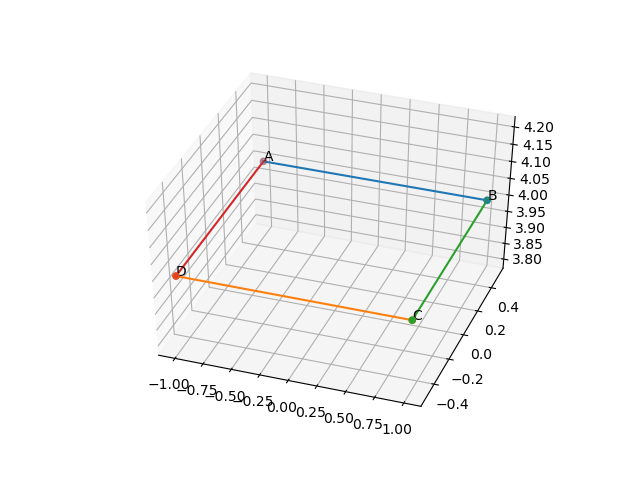
\includegraphics[width=\columnwidth]{chapters/12/10/4/12/figs/Figure_1.png}
   \caption{}
   \label{fig:chapters/12/10/4/12Rect_ABCD}
\end{figure}





\item Find the area of the triangle whose vertices are 
\begin{enumerate}
\item $(2, 3), (–1, 0), (2, – 4)$
\item $(–5, –1), (3, –5), (5, 2)$ 
\end{enumerate}
		\label{10/7/3/1}
\solution
		    See \tabref{eq:10/7/3/1/area}.
\begin{table}[H]
    \centering
    \caption{}
    \label{eq:10/7/3/1/area}
    \begin{tabular}{|c|c|c|c|}
        \hline
	     & $\vec{A}-\vec{B}$  & $\vec{A}-\vec{C}$  & $\frac{1}{2}\|\brak{\vec{A}-\vec{B}} \times \brak{\vec{A}-\vec{C}}\|$ \\
        \hline
         a)& $\myvec{ 3 \\3 }$ & $\myvec{ 0 \\ 7 }$ & $\frac{21}{2}$ \\
        \hline
	    b)& $\myvec{
 -8 \\
 4 
 }$
         &$\myvec{
 -10 \\
 -3 
 }$
  &  $32$   \\
        \hline
    \end{tabular}
\end{table}


\item Find the area of the triangle formed by joining the mid-points of the sides of the triangle whose vertices are $A(0, –1), B(2, 1)$  and  $C(0, 3)$. Find the ratio of this area to the area of the given triangle.
	\\
\solution
		Using 
	  \eqref{eq:section_formula},
the mid point coordinates are given by
	\begin{align}
		\vec{P} = \frac{1}{2}\vec(\vec{A}+\vec{B})  = \myvec{1\\0}\\
		\vec{Q} = \frac{1}{2}\vec(\vec{B}+\vec{C}) = \myvec{1\\2}\\
		\vec{R} = \frac{1}{2}\vec(\vec{A}+\vec{C}) = \myvec{0\\1}
	\end{align}
	\begin{align}
\because		\vec{P}-\vec{Q} =  \myvec{
 0 \\
 -2 
 },\,
		\vec{Q}-\vec{R} =   \myvec{
 1 \\
 1 
 }
 \\
		ar(PQR)=\frac{1}{2}{\norm{\vec(\vec{P}-\vec{Q})\times\vec(\vec{Q}-\vec{R})}}
		=1
	\end{align}
	Similarly, 
	\begin{align}
		\vec{A}-\vec{B} = \myvec{
 -2 \\
 -2 
 }
 ,\,
		\vec{A}-\vec{C} =  \myvec{
 0 \\
 -4 
 }
 \\
 \implies
		ar(ABC)=\frac{1}{2}{\norm{\vec(\vec{A}-\vec{B})\times\vec(\vec{A}-\vec{C})}}
=4
\\
		\implies \frac{ar\brak{PQR}}{ar\brak{ABC}} = \frac{1}{4}
	\end{align}
	See 
\figref{fig:10/7/3/3Fig}
\begin{figure}[H]
	\begin{center} 
	    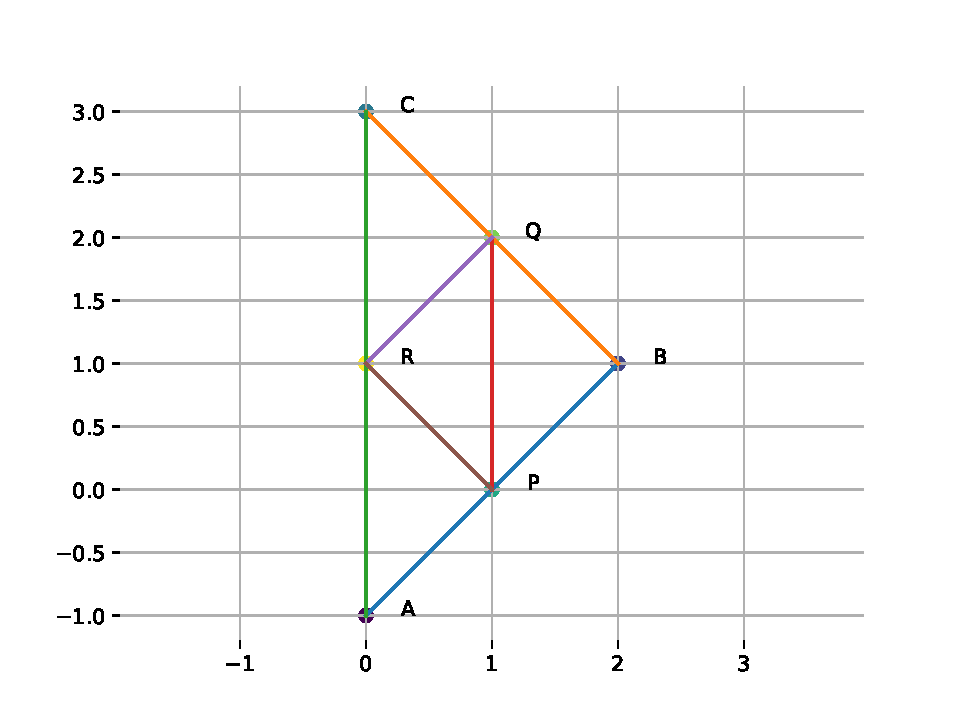
\includegraphics[width=0.75\columnwidth]{chapters/10/7/3/3/figs/fig.pdf}
	\end{center}
\caption{}
\label{fig:10/7/3/3Fig}
\end{figure}


\item Find the area of the quadrilateral whose vertices, taken in order, are $A(– 4, – 2), B(– 3, – 5), C(3, – 2)$  and $ D(2, 3)$.
	\\
\solution
		\iffalse
\documentclass[12pt]{article}
\usepackage{graphicx}
%\documentclass[journal,12pt,twocolumn]{IEEEtran}
\usepackage[none]{hyphenat}
\usepackage{graphicx}
\usepackage{listings}
\usepackage[english]{babel}
\usepackage{graphicx}
\usepackage{caption} 
\usepackage{hyperref}
\usepackage{booktabs}
\def\inputGnumericTable{}
\usepackage{color}                                            %%
    \usepackage{array}                                            %%
    \usepackage{longtable}                                        %%
    \usepackage{calc}                                             %%
    \usepackage{multirow}                                         %%
    \usepackage{hhline}                                           %%
    \usepackage{ifthen}
\usepackage{array}
\usepackage{amsmath}   % for having text in math mode
\usepackage{listings}
\lstset{
language=tex,
frame=single, 
breaklines=true
}
  
%Following 2 lines were added to remove the blank page at the beginning
\usepackage{atbegshi}% http://ctan.org/pkg/atbegshi
\AtBeginDocument{\AtBeginShipoutNext{\AtBeginShipoutDiscard}}
%
%New macro definitions
\newcommand{\mydet}[1]{\ensuremath{\begin{vmatrix}#1\end{vmatrix}}}
\providecommand{\brak}[1]{\ensuremath{\left(#1\right)}}
\providecommand{\norm}[1]{\left\lVert#1\right\rVert}
\newcommand{\solution}{\noindent \textbf{Solution: }}
\newcommand{\myvec}[1]{\ensuremath{\begin{pmatrix}#1\end{pmatrix}}}
\let\vec\mathbf
\begin{document}
\begin{center}
\title{\textbf{Coordinate Geometry}}
\date{\vspace{-5ex}} %Not to print date automatically
\maketitle
\end{center}
\setcounter{page}{1}
\section*{10$^{th}$ Maths - Chapter 7}
This is Problem-4 from Exercise 7.3
\begin{enumerate}
\item Find the area of quadrilateral whose vertices, taken in order, are $\myvec{-4 \\ -2}, \myvec{-3\\-5}, \myvec{3\\-2}$ and $\myvec{2\\3}$.\\
	\solution 
\fi
		The input parameters for this problem are available in Table \eqref{tab:10/7/3/4}.
\begin{table}[ht!]\centering
%%%%%%%%%%%%%%%%%%%%%%%%%%%%%%%%%%%%%%%%%%%%%%%%%%%%%%%%%%%%%%%%%%%%%%
%%                                                                  %%
%%  This is the header of a LaTeX2e file exported from Gnumeric.    %%
%%                                                                  %%
%%  This file can be compiled as it stands or included in another   %%
%%  LaTeX document. The table is based on the longtable package so  %%
%%  the longtable options (headers, footers...) can be set in the   %%
%%  preamble section below (see PRAMBLE).                           %%
%%                                                                  %%
%%  To include the file in another, the following two lines must be %%
%%  in the including file:                                          %%
%%        \def\inputGnumericTable{}                                 %%
%%  at the beginning of the file and:                               %%
%%        \input{name-of-this-file.tex}                             %%
%%  where the table is to be placed. Note also that the including   %%
%%  file must use the following packages for the table to be        %%
%%  rendered correctly:                                             %%
%%    \usepackage[latin1]{inputenc}                                 %%
%%    \usepackage{color}                                            %%
%%    \usepackage{array}                                            %%
%%    \usepackage{longtable}                                        %%
%%    \usepackage{calc}                                             %%
%%    \usepackage{multirow}                                         %%
%%    \usepackage{hhline}                                           %%
%%    \usepackage{ifthen}                                           %%
%%  optionally (for landscape tables embedded in another document): %%
%%    \usepackage{lscape}                                           %%
%%                                                                  %%
%%%%%%%%%%%%%%%%%%%%%%%%%%%%%%%%%%%%%%%%%%%%%%%%%%%%%%%%%%%%%%%%%%%%%%



%%  This section checks if we are begin input into another file or  %%
%%  the file will be compiled alone. First use a macro taken from   %%
%%  the TeXbook ex 7.7 (suggestion of Han-Wen Nienhuys).            %%
\def\ifundefined#1{\expandafter\ifx\csname#1\endcsname\relax}


%%  Check for the \def token for inputed files. If it is not        %%
%%  defined, the file will be processed as a standalone and the     %%
%%  preamble will be used.                                          %%
\ifundefined{inputGnumericTable}

%%  We must be able to close or not the document at the end.        %%
 \def\gnumericTableEnd{\end{document}}


%%%%%%%%%%%%%%%%%%%%%%%%%%%%%%%%%%%%%%%%%%%%%%%%%%%%%%%%%%%%%%%%%%%%%%
%%                                                                  %%
%%  This is the PREAMBLE. Change these values to get the right      %%
%%  paper size and other niceties.                                  %%
%%                                                                  %%
%%%%%%%%%%%%%%%%%%%%%%%%%%%%%%%%%%%%%%%%%%%%%%%%%%%%%%%%%%%%%%%%%%%%%%

 \documentclass[12pt%
     %,landscape%
                    ]{report}
       \usepackage[latin1]{inputenc}
       \usepackage{fullpage}
       \usepackage{color}
       \usepackage{array}
       \usepackage{longtable}
       \usepackage{calc}
       \usepackage{multirow}
       \usepackage{hhline}
       \usepackage{ifthen}

 \begin{document}


%%  End of the preamble for the standalone. The next section is for %%
%%  documents which are included into other LaTeX2e files.          %%
\else

%%  We are not a stand alone document. For a regular table, we will %%
%%  have no preamble and only define the closing to mean nothing.   %%
    \def\gnumericTableEnd{}

%%  If we want landscape mode in an embedded document, comment out  %%
%%  the line above and uncomment the two below. The table will      %%
%%  begin on a new page and run in landscape mode.                  %%
%       \def\gnumericTableEnd{\end{landscape}}
%       \begin{landscape}


%%  End  theoelse clause for this file being \input.              %%
\fi

%%%%%%%%%%%%%%%%%%%%%%%%%%%%%%%%%%%%%%%%%%%%%%%%%%%%%%%%%%%%%%%%%%%%%%
%%                                                                  %%
%%  The rest is the gnumeric table, except for the closing          %%
%%  statement. Changes below will alter the table's appearance.     %%
%%                                                                  %%
%%%%%%%%%%%%%%%%%%%%%%%%%%%%%%%%%%%%%%%%%%%%%%%%%%%%%%%%%%%%%%%%%%%%%%

\providecommand{\gnumericmathit}[1]{#1} 
%%  Uncomment the next line if you would like your numbers to be in %%
%%  italics if they are italizised in the gnumeric table.           %%
%\renewcommand{\gnumericmathit}[1]{\mathit{#1}}
\providecommand{\gnumericPB}[1]%
{\let\gnumericTemp=\\#1\let\\=\gnumericTemp\hspace{0pt}}
 \ifundefined{gnumericTableWidthDefined}
        \newlength{\gnumericTableWidth}
        \newlength{\gnumericTableWidthComplete}
        \newlength{\gnumericMultiRowLength}
        \global\def\gnumericTableWidthDefined{}
 \fi
%% The following setting protects this code from babel shorthands.  %%
 \ifthenelse{\isundefined{\languageshorthands}}{}{\languageshorthands{english}}
%%  The default table format retains the relative column widths of  %%
%%  gnumeric. They can easily be changed to c, r or l. In that case %%
%%  you may want to comment out the next line and uncomment the one %%
%%  thereafter                                                      %%
\providecommand\gnumbox{\makebox[0pt]}
%%\providecommand\gnumbox[1][]{\makebox}

%% to adjust positions in multirow situations                       %%
\setlength{\bigstrutjot}{\jot}
\setlength{\extrarowheight}{\doublerulesep}

%%  The \setlongtables command keeps column widths the same across  %%
%%  pages. Simply comment out next line for varying column widths.  %%
\setlongtables

\setlength\gnumericTableWidth{%
 53pt+%
 53pt+%
 82pt+%
 53pt+%
0pt}
\def\gumericNumCols{4}
\setlength\gnumericTableWidthComplete{\gnumericTableWidth+%
         \tabcolsep*\gumericNumCols*2+\arrayrulewidth*\gumericNumCols}
\ifthenelse{\lengthtest{\gnumericTableWidthComplete > \linewidth}}%
         {\def\gnumericScale{1*\ratio{\linewidth-%
                        \tabcolsep*\gumericNumCols*2-%
                        \arrayrulewidth*\gumericNumCols}%
{\gnumericTableWidth}}}%
{\def\gnumericScale{1}}

%%%%%%%%%%%%%%%%%%%%%%%%%%%%%%%%%%%%%%%%%%%%%%%%%%%%%%%%%%%%%%%%%%%%%%
%%                                                                  %%
%% The following are the widths of the various columns. We are      %%
%% defining them here because then they are easier to change.       %%
%% Depending on the cell formats we may use them more than once.    %%
%%                                                                  %%
%%%%%%%%%%%%%%%%%%%%%%%%%%%%%%%%%%%%%%%%%%%%%%%%%%%%%%%%%%%%%%%%%%%%%%

\ifthenelse{\isundefined{\gnumericColA}}{\newlength{\gnumericColA}}{}\settowidth{\gnumericColA}{\begin{tabular}{@{}p{53pt*\gnumericScale}@{}}x\end{tabular}}
\ifthenelse{\isundefined{\gnumericColB}}{\newlength{\gnumericColB}}{}\settowidth{\gnumericColB}{\begin{tabular}{@{}p{53pt*\gnumericScale}@{}}x\end{tabular}}
\ifthenelse{\isundefined{\gnumericColC}}{\newlength{\gnumericColC}}{}\settowidth{\gnumericColC}{\begin{tabular}{@{}p{82pt*\gnumericScale}@{}}x\end{tabular}}
\ifthenelse{\isundefined{\gnumericColD}}{\newlength{\gnumericColD}}{}\settowidth{\gnumericColD}{\begin{tabular}{@{}p{53pt*\gnumericScale}@{}}x\end{tabular}}

\begin{center}
\begin{tabular}[c]{%
 b{\gnumericColA}%
 b{\gnumericColB}%
 b{\gnumericColC}%
 b{\gnumericColD}%
 }

%%%%%%%%%%%%%%%%%%%%%%%%%%%%%%%%%%%%%%%%%%%%%%%%%%%%%%%%%%%%%%%%%%%%%%
%%  The longtable options. (Caption, headers... see Goosens, p.124) %%
% \caption{The Table Caption.}             \\ %
% \hline % Across the top of the table.
%%  The rest of these options are table rows which are placed on    %%
%%  the first, last or every page. Use \multicolumn if you want.    %%

%%  Header for the first page.                                      %%
% \multicolumn{4}{c}{The First Header} \\ \hline 
% \multicolumn{1}{c}{colTag} %Column 1
% &\multicolumn{1}{c}{colTag} %Column 2
% &\multicolumn{1}{c}{colTag} %Column 3
% &\multicolumn{1}{c}{colTag} \\ \hline %Last column
% \endfirsthead

%%  The running header definition.                                  %%
% \hline
% \multicolumn{4}{l}{\ldots\small\slshape continued} \\ \hline
% \multicolumn{1}{c}{colTag} %Column 1
% &\multicolumn{1}{c}{colTag} %Column 2
% &\multicolumn{1}{c}{colTag} %Column 3
% &\multicolumn{1}{c}{colTag} \\ \hline %Last column
% \endhead

%%  The running footer definition.                                  %%
% \hline
% \multicolumn{4}{r}{\small\slshape continued\ldots} \\
% \endfoot

%%  The ending footer definition.                                   %%
% \multicolumn{4}{c}{That's all folks} \\ \hline 
% \endlastfoot
%%%%%%%%%%%%%%%%%%%%%%%%%%%%%%%%%%%%%%%%%%%%%%%%%%%%%%%%%%%%%%%%%%%%%%

\hhline{|-|-|-~}
  \multicolumn{1}{|p{\gnumericColA}|}%
 {\gnumericPB{\centering}\gnumbox{\textbf{Symbol}}}
 &\multicolumn{1}{p{\gnumericColB}|}%
 {\gnumericPB{\centering}\gnumbox{\textbf{Value}}}
 &\multicolumn{1}{p{\gnumericColC}|}%
 {\gnumericPB{\centering}\gnumbox{\textbf{Description}}}
 &
\\
\hhline{|---|~}
  \multicolumn{1}{|p{\gnumericColA}|}%
 {\gnumericPB{\centering}\gnumbox{$\vec{A}$}}
 &\multicolumn{1}{p{\gnumericColB}|}%
 {\gnumericPB{\centering}\gnumbox{$\myvec{-4\\-2}$}}
 &\multicolumn{1}{p{\gnumericColC}|}%
 {\gnumericPB{\centering}\gnumbox{First point}}
 &
\\
\hhline{|---|~}
  \multicolumn{1}{|p{\gnumericColA}|}%
 {\gnumericPB{\centering}\gnumbox{$\vec{B}$}}
 &\multicolumn{1}{p{\gnumericColB}|}%
 {\gnumericPB{\centering}\gnumbox{$\myvec{-3\\-5}$}}
 &\multicolumn{1}{p{\gnumericColC}|}%
 {\gnumericPB{\centering}\gnumbox{Second point}}
 &
\\
\hhline{|---|~}
  \multicolumn{1}{|p{\gnumericColA}|}%
 {\gnumericPB{\centering}\gnumbox{$\vec{C}$}}
 &\multicolumn{1}{p{\gnumericColB}|}%
 {\gnumericPB{\centering}\gnumbox{$\myvec{3\\-2}$}}
 &\multicolumn{1}{p{\gnumericColC}|}%
 {\gnumericPB{\centering}\gnumbox{Third point}}
 &
\\

\hhline{|---|~}
  \multicolumn{1}{|p{\gnumericColA}|}%
 {\gnumericPB{\centering}\gnumbox{$\vec{D}$}}
 &\multicolumn{1}{p{\gnumericColB}|}%
 {\gnumericPB{\centering}\gnumbox{$\myvec{2\\3}$}}
 &\multicolumn{1}{p{\gnumericColC}|}%
 {\gnumericPB{\centering}\gnumbox{Fourth point}}
 &
\\
\hhline{|-|-|-|~}
\end{tabular}
 \end{center}

\ifthenelse{\isundefined{\languageshorthands}}{}{\languageshorthands{\languagename}}
%\gnumericTableEndf

\caption{}
\label{tab:10/7/3/4}	
\end{table}
By joining $\vec{B}$ to $\vec{D}$, two triangles $\vec{A}\vec{B}\vec{D}$ and $\vec{B}\vec{C}\vec{D}$ are obtained.
Since
\begin{align}
	\vec{A}- \vec{B} &= \myvec{-4\\-2\\}-\myvec{-3\\-5\\}=\myvec{-1\\3\\}\label{eq:chapters/10/7/3/4/2}\\
	  \vec{A}- \vec{D} &= \myvec{-4\\-2\\}-\myvec{2\\3\\}=\myvec{-6\\-5\\}\label{eq:chapters/10/7/3/4/3}
  \end{align}
  \begin{align}
	  ar(ABD)&=\frac{1}{2} \norm{\brak{\vec{A}-\vec{B}}  \times 
   \brak{\vec{A}- \vec{D}}} \label{eq:chapters/10/7/3/4/1} 
   \\
	  &=	\frac{1}{2}\mydet{-1 & 3\\-6 & -5}  
	=	\frac{23}{2}
\end{align}
upon substituting the values of \eqref{eq:chapters/10/7/3/4/2} and \eqref{eq:chapters/10/7/3/4/3} in \eqref{eq:chapters/10/7/3/4/1}.
Similarly,
\begin{align}
	\vec{B}- \vec{C} &= \myvec{-3\\-5\\}-\myvec{3\\-2\\}=\myvec{-6\\-5\\}\label{eq:chapters/10/7/3/4/6} \\
	  \vec{B}- \vec{D} &= \myvec{-3\\-5\\}-\myvec{2\\3\\}=\myvec{-3\\-8\\}\label{eq:chapters/10/7/3/4/7} 
  \end{align}
  yielding
  \begin{align}
	  ar(BCD)&=\frac{1}{2} \norm{\brak{\vec{B}-\vec{C}}  \times 
   \brak{\vec{B}- \vec{D}}} \label{eq:chapters/10/7/3/4/5}
   \\
	  &=	\frac{1}{2}\mydet{-6 & -3\\-5 & -8}  
	=	\frac{33}{2}
\end{align}
	upon 	substituting the values of \eqref{eq:chapters/10/7/3/4/6} and \eqref{eq:chapters/10/7/3/4/7} in \eqref{eq:chapters/10/7/3/4/5}
		Thus, 
\begin{align}
	ar(ABCD)&=  ar(ABD) +  ar(BCD)
	= 28
\end{align}
See Fig. 
\ref{fig:chapters/10/7/3/4/Fig1}
\begin{figure}[!h]
 \begin{center}
  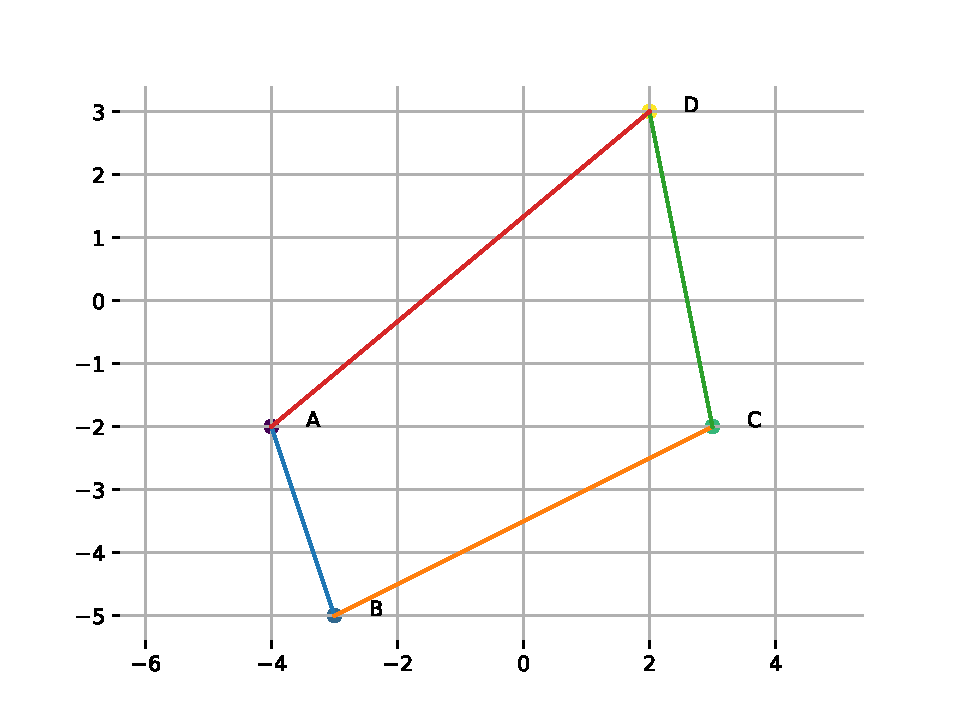
\includegraphics[width=\columnwidth]{chapters/10/7/3/4/figs/fig.pdf}
 \end{center}
\caption{}
\label{fig:chapters/10/7/3/4/Fig1}
\end{figure}


\item Verify that a median of a triangle divides it into two triangles of equal areas for $\triangle ABC$ whose vertices are $\vec{A}(4, -6), \vec{B}(3, 2), \text{ and } \vec{C}(5, 2)$. 
		\label{10/7/3/5}
		\\
\solution
		\begin{align}
\vec{D}=\frac{\vec{B}+\vec{C}}{2}
=\myvec{4\\ 0},
\\
	\vec{A}- \vec{B} =\myvec{1\\ -4},\,
	  \vec{A}- \vec{D} =\myvec{0\\ -6}
	  \\
	  \implies
  ar(ABD)=\frac{1}{2} \norm{\brak{\vec{A}-\vec{B}}  \times 
   \brak{\vec{A}- \vec{D}}} 
	       =3	
	       \\
	\vec{A}- \vec{C} =\myvec{-1\\ -8},\,
	  \vec{A}- \vec{D} =\myvec{0\\ -6}
	  \\
	  \implies
  ar(ACD)=\frac{1}{2} \norm{\brak{\vec{A}-\vec{C}}  \times 
   \brak{\vec{A}- \vec{D}}} 
   \\
	= 3 =
ar(ABD)
\end{align}
See  
\figref{fig:10/7/3/5/}.
\begin{figure}[H]
\centering
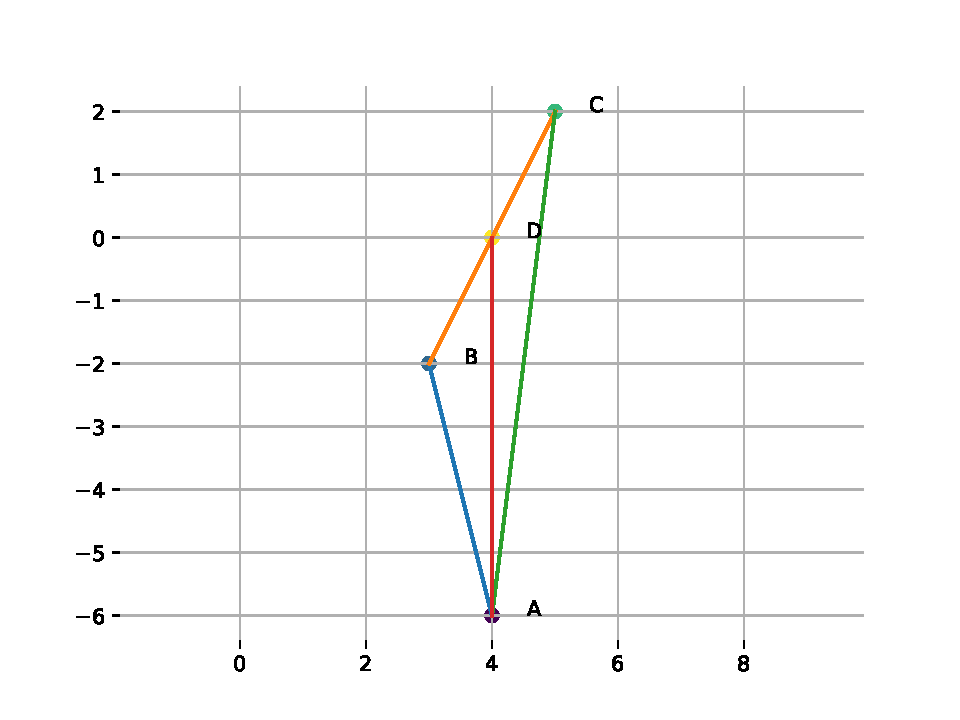
\includegraphics[width=0.75\columnwidth]{chapters/10/7/3/5/figs/fig.pdf}
\caption{}
\label{fig:10/7/3/5/}
\end{figure} 

\item The two adjacent sides of a parallelogram are 
$\vec{a}= 2\hat{i}-4\hat{j}+5\hat{k}$  and  $\vec{b} =\hat{i}-2\hat{j}-3\hat{k}$.
Find the unit vector parallel to its diagonal. Also, find its area.\\
	\solution
		\iffalse
\documentclass[journal,12pt,twocolumn]{IEEEtran}
\usepackage{setspace}
\usepackage{gensymb}
\usepackage{xcolor}
\usepackage{caption}
\singlespacing
\usepackage{siunitx}
\usepackage[cmex10]{amsmath}
\usepackage{mathtools}
\usepackage{hyperref}
\usepackage{amsthm}
\usepackage{mathrsfs}
\usepackage{txfonts}
\usepackage{stfloats}
\usepackage{cite}
\usepackage{cases}
\usepackage{subfig}
\usepackage{longtable}
\usepackage{multirow}
\usepackage{enumitem}
\usepackage{bm}
\usepackage{mathtools}
\usepackage{listings}
\usepackage{tikz}
\usetikzlibrary{shapes,arrows,positioning}
\usepackage{circuitikz}
\renewcommand{\vec}[1]{\boldsymbol{\mathbf{#1}}}
\DeclareMathOperator*{\Res}{Res}
\renewcommand\thesection{\arabic{section}}
\renewcommand\thesubsection{\thesection.\arabic{subsection}}
\renewcommand\thesubsubsection{\thesubsection.\arabic{subsubsection}}

\renewcommand\thesectiondis{\arabic{section}}
\renewcommand\thesubsectiondis{\thesectiondis.\arabic{subsection}}
\renewcommand\thesubsubsectiondis{\thesubsectiondis.\arabic{subsubsection}}
\hyphenation{op-tical net-works semi-conduc-tor}

\lstset{
language=Python,
frame=single, 
breaklines=true,
columns=fullflexible
}
\begin{document}
\theoremstyle{definition}
\newtheorem{theorem}{Theorem}[section]
\newtheorem{problem}{Problem}
\newtheorem{proposition}{Proposition}[section]
\newtheorem{lemma}{Lemma}[section]
\newtheorem{corollary}[theorem]{Corollary}
\newtheorem{example}{Example}[section]
\newtheorem{definition}{Definition}[section]
\newcommand{\BEQA}{\begin{eqnarray}}
        \newcommand{\EEQA}{\end{eqnarray}}
\newcommand{\define}{\stackrel{\triangle}{=}}
\newcommand{\myvec}[1]{\ensuremath{\begin{pmatrix}#1\end{pmatrix}}}
\newcommand{\mydet}[1]{\ensuremath{\begin{vmatrix}#1\end{vmatrix}}}
\bibliographystyle{IEEEtran}
\providecommand{\nCr}[2]{\,^{#1}C_{#2}} % nCr
\providecommand{\nPr}[2]{\,^{#1}P_{#2}} % nPr
\providecommand{\mbf}{\mathbf}
\providecommand{\pr}[1]{\ensuremath{\Pr\left(#1\right)}}
\providecommand{\qfunc}[1]{\ensuremath{Q\left(#1\right)}}
\providecommand{\sbrak}[1]{\ensuremath{{}\left[#1\right]}}
\providecommand{\lsbrak}[1]{\ensuremath{{}\left[#1\right.}}
\providecommand{\rsbrak}[1]{\ensuremath{{}\left.#1\right]}}
\providecommand{\brak}[1]{\ensuremath{\left(#1\right)}}
\providecommand{\lbrak}[1]{\ensuremath{\left(#1\right.}}
\providecommand{\rbrak}[1]{\ensuremath{\left.#1\right)}}
\providecommand{\cbrak}[1]{\ensuremath{\left\{#1\right\}}}
\providecommand{\lcbrak}[1]{\ensuremath{\left\{#1\right.}}
\providecommand{\rcbrak}[1]{\ensuremath{\left.#1\right\}}}
\theoremstyle{remark}
\newtheorem{rem}{Remark}
\newcommand{\sgn}{\mathop{\mathrm{sgn}}}
\newcommand{\rect}{\mathop{\mathrm{rect}}}
\newcommand{\sinc}{\mathop{\mathrm{sinc}}}
\providecommand{\abs}[1]{\left\vert#1\right\vert}
\providecommand{\res}[1]{\Res\displaylimits_{#1}}
\providecommand{\norm}[1]{\lVert#1\rVert}
\providecommand{\mtx}[1]{\mathbf{#1}}
\providecommand{\mean}[1]{E\left[ #1 \right]}
\providecommand{\fourier}{\overset{\mathcal{F}}{ \rightleftharpoons}}
\providecommand{\ztrans}{\overset{\mathcal{Z}}{ \rightleftharpoons}}
\providecommand{\system}[1]{\overset{\mathcal{#1}}{ \longleftrightarrow}}
\newcommand{\solution}{\noindent \textbf{Solution: }}
\providecommand{\dec}[2]{\ensuremath{\overset{#1}{\underset{#2}{\gtrless}}}}
\let\StandardTheFigure\thefigure
\def\putbox#1#2#3{\makebox[0in][l]{\makebox[#1][l]{}\raisebox{\baselineskip}[0in][0in]{\raisebox{#2}[0in][0in]{#3}}}}
\def\rightbox#1{\makebox[0in][r]{#1}}
\def\centbox#1{\makebox[0in]{#1}}
\def\topbox#1{\raisebox{-\baselineskip}[0in][0in]{#1}}
\def\midbox#1{\raisebox{-0.5\baselineskip}[0in][0in]{#1}}

\vspace{3cm}
\title{12.10.5.10}
\author{Lokesh Surana}
\maketitle
\section*{Class 12, Chapter 10, Exercise 5.10}

Q.10. The two adjacent sides of a parallelogram are  ${2}\hat{i} -  {4}\hat{j} + {5}\hat{k}$ and ${1}\hat{i} -  {2}\hat{j} - {3}\hat{k}$.
Find the unit vector parallel to its diagonal. Also, find its area.

\solution 
\fi
Let the sides of the parallelogram be 
\begin{align}
\vec{a} = \myvec{2\\-4\\5}, \, \vec{b} = \myvec{1\\-2\\-3}.
\end{align}
The diagonals of the parallelogram are given by
\begin{align}
	\vec{D}_1 &= \vec{a} + \vec{b} = \myvec{3 \\-6\\2} \\
	\vec{D}_2 &= \vec{a} - \vec{b} = \myvec{1 \\-2\\8}
\end{align}
The unit vectors parallel to the diagonals are then given by
\begin{align}
	\hat{\vec{D}_1} &= \frac{\vec{D}_1}{\norm{\vec{D}_1}}  = \myvec{\frac{3}{\sqrt{45}}\\-\frac{6}{\sqrt{45}}\\\frac{2}{\sqrt{45}}} \\
    \hat{\vec{D}_2} &= \frac{\vec{D}_2}{\norm{\vec{D}_2}}  = \myvec{\frac{1}{\sqrt{69}}\\-\frac{2}{\sqrt{69}}\\\frac{8}{\sqrt{69}}}
\end{align}
%
Since
\begin{align}
    \vec{a}\times\vec{b}=\myvec{22 \\-11\\0},
\end{align}
he area of the parallelogram is given by
\begin{align}
    \norm{\vec{a}\times\vec{b}}  = \sqrt{605}
\end{align}


\item The vertices of a $\triangle ABC$ are $\vec{A}(4,6), \vec{B}(1,5)$ and  $\vec{C}(7,2)$. A line is drawn to intersect sides $AB$ and $AC$ at $\vec{D}$ and $\vec{E}$ respectively, such that $\frac{AD}{AB} = \frac{AE}{AC} = \frac{1}{4}$. Calculate the area of $\triangle ADE$ and compare it with the area of the $\triangle ABC$.
\\
\solution
	See  
\figref{fig:chapters/10/7/4/6Fig1}.
\begin{figure}[H]
 \begin{center}
 \includegraphics[width=0.75\columnwidth]{chapters/10/7/4/6/figs/fig.pdf}
 \end{center}
\caption{}
\label{fig:chapters/10/7/4/6Fig1}
\end{figure}
	Using section formula
	  \eqref{eq:section_formula},
\begin{align}
\vec{D} =\frac{3\vec{A}+\vec{B}}{4}
	=\frac{1}{4}\myvec{13\\ 23}
	\\
\vec{E} =\frac{3\vec{A}+\vec{C}}{4}
	=\frac{1}{4}\myvec{19\\ 20}
	\\
	\vec{A}- \vec{D} 
	=\frac{1}{4}\myvec{3\\ 1},\,
	  \vec{A}- \vec{E}  
	=\frac{1}{4}\myvec{-3\\ 1}
	\\
	\vec{A}- \vec{B} =\myvec{3\\1},
	  \vec{B}-\vec{C} =\myvec{-6\\3}
\end{align}
yielding
\begin{align}
ar(ABD) =\frac{1}{2} \norm{\brak{\vec{A}-\vec{D}}  \times 
   \brak{\vec{A}- \vec{E}}} 
	=	\frac{15}{32}
	\\
	  ar(ABC) =\frac{1}{2} \norm{\brak{\vec{A}-\vec{B}}  \times 
   \brak{\vec{B}- \vec{C}}} 
	=	\frac{15}{2}
	\\
	\implies \frac{ar\brak{ADE}}{ar\brak{ABC}}=\frac{1}{16}
\end{align}

    \item Draw a quadrilateral in the Cartesian plane, whose vertices are 
    \begin{align}
        \vec{A} = \myvec{-4\\5},\, \vec{B} = \myvec{0\\7},\, 
        \vec{C} = \myvec{5\\-5},\, \vec{D} = \myvec{-4\\-2}.
    \end{align}
    Also, find its area.
\label{chapters/11/10/1/1}
   \\ 
    \solution 
See \figref{fig:11/10/1/1quad}.
    From 
        \eqref{eq:11/10/1/1area-diag},
    \begin{align}
ar\brak{ABCD}
	       = \frac{121}{2}
        \label{eq:11/10/1/1ans}
    \end{align}
    \begin{figure}[H]
        \centering
        \includegraphics[width=0.75\columnwidth]{chapters/11/10/1/1/figs/fig.pdf}
        \caption{Plot of quadrilateral $ABCD$}
        \label{fig:11/10/1/1quad}
    \end{figure}

\item Find the area of region bounded by the triangle whose
	vertices are $(1, 0), (2, 2) \text{ and } (3, 1)$. 
\item Find the area of region bounded by the triangle whose vertices
	are $(– 1, 0), (1, 3) \text{ and } (3, 2)$. 
\item Find the area of the $\triangle ABC$, coordinates of whose vertices are $\vec{A}(2, 0), \vec{B}(4, 5), \text{ and } \vec{C}(6, 3)$.
\item Show that $$(\overrightarrow{a}-\overrightarrow{b})\times (\overrightarrow{a}+\overrightarrow{b})=2(\overrightarrow{a}\times \overrightarrow{b})$$
	\\
		\solution
		\iffalse
\documentclass[journal,12pt,twocolumn]{IEEEtran}
\usepackage{graphicx}
\graphicspath{{./figs/}}{}
\usepackage{amsmath,amssymb,amsfonts,amsthm}
\newcommand{\myvec}[1]{\ensuremath{\begin{pmatrix}#1\end{pmatrix}}}
\providecommand{\norm}[1]{\lVert#1\rVert}
\usepackage{listings}
\usepackage{watermark}
\usepackage{titlesec}
\usepackage{caption}
\newcommand{\mydet}[1]{\ensuremath{\begin{vmatrix}#1\end{vmatrix}}}
\let\vec\mathbf
\lstset{
frame=single, 
breaklines=true,
columns=fullflexible
}
\thiswatermark{\centering \put(0,-105.0){\includegraphics[scale=0.15]{/sdcard/IITH/vectors/12.10.4.4/figs/logo.png}} }
\title{\mytitle}
\title{
Assignment - 12.10.4.4
}
\author{Surajit Sarkar}
\begin{document}
\maketitle
\tableofcontents
\bigskip
\section{\textbf{Problem}}
Show that $\myvec{\vec{a}-\vec{b}}\times\myvec{\vec{a}+\vec{b}}=2\myvec{\vec{a}\times\vec{b}}$
\section{\textbf{Solution}}
\fi
Consider
\begin{align}
\vec{a}=\myvec{1\\1},\vec{b}&=\myvec{2\\1}
\end{align}
Then
  \begin{align}
  \myvec{\vec{a}-\vec{b}}&=\myvec{-1\\0}
  \myvec{\vec{a}+\vec{b}}=\myvec{3\\2}\\
\implies \myvec{\vec{a}-\vec{b}}\times\myvec{\vec{a}+\vec{b}}
  &=\mydet{-1 & 3\\0 & 2} 
  =-2
\end{align}
and 
\begin{align}
  2\myvec{\vec{a}\times\vec{b}}
  =2\mydet{1 & 2\\0 & 1}
  =-2
  \end{align}

\item If either $\overrightarrow{a} = \overrightarrow{0}$ or $\overrightarrow{b} = \overrightarrow{0}$, then $\overrightarrow{a} \times \overrightarrow{b} = \overrightarrow{0}$. Is the converse true? Justify your answer with an example.
	\\
		\solution
		For
\begin{align}
\vec{a} = \myvec{1 \\ 0 \\ 0},\, \vec{b} = \myvec{2 \\ 0 \\ 0}
\\
   \vec{a} \times \vec{b} = \vec{0}. 
\end{align}


\item Given that $\overrightarrow{a} \cdot \overrightarrow{b} = 0$ and $\overrightarrow{a} \times \overrightarrow{b} = \overrightarrow{0}$. What can you conclude about the vectors $\overrightarrow{a} \text{ and }\overrightarrow{b}$?
\end{enumerate}


\newpage
\subsection{Miscellaneous}
\begin{enumerate}[label=\thesubsection.\arabic*,ref=\thesubsection.\theenumi]
\item The two opposite vertices of a square are $(–1, 2)$  and $ (3, 2)$. Find the coordinates of the other two vertices.
\\
\solution
	\iffalse
\documentclass[12pt]{article}
\usepackage{graphicx}
\usepackage{amsmath}
\usepackage{mathtools}
\usepackage{gensymb}

\newcommand{\mydet}[1]{\ensuremath{\begin{vmatrix}#1\end{vmatrix}}}
\providecommand{\brak}[1]{\ensuremath{\left(#1\right)}}
\providecommand{\norm}[1]{\left\lVert#1\right\rVert}
\newcommand{\solution}{\noindent \textbf{Solution: }}
\newcommand{\myvec}[1]{\ensuremath{\begin{pmatrix}#1\end{pmatrix}}}
\let\vec\mathbf

\begin{document}
\begin{center}
\textbf\large{CHAPTER-7 \\ COORDINATE GEOMETRY}

\end{center}
\section*{Excercise 7.4}

Q4.The two opposite vertices of a square are $(–1, 2) \text{ and } (3, 2)$. Find the coordinates of the other two vertices.\\
\fi
\solution
Let
\begin{align}
\vec{A} = \myvec
{
-1 \\
 2\\
},
\vec{C} = 
\myvec
{
3\\
2\\
}
\end{align}

\begin{figure}[!h]
	\begin{center} 
	    \includegraphics[width=\columnwidth]{chapters/10/7/4/4/figs/square}
	\end{center}
\caption{}
\label{fig:7/4/4/4Fig1}
\end{figure}

Shifting $\vec{A}$ to origin with reference to Fig. \ref{fig:7/4/4/4Fig2},
\begin{align}
\vec{A^{\prime}} =
\myvec{
0 \\
0\\
},
\vec{C^{\prime}} = \vec{C}-\vec{A} = 
\myvec{
4 \\
0\\
}
\end{align}

\begin{figure}[!h]
	\begin{center} 
	    \includegraphics[width=\columnwidth]{chapters/10/7/4/4/figs/square1}
	\end{center}
\caption{}
\label{fig:7/4/4/4Fig2}
\end{figure}
\iffalse
In general,
the angle made by $AC$ with the x-axis is 
		\begin{align}
\beta = \theta + 45\degree
		\end{align}
\fi
Since
\begin{align}
\vec{C} - \vec{A} = \myvec{
4\\
0
} \equiv 
\myvec{
1\\
0
},
	\tan\theta&= \frac{0}{4} \implies 
\theta= 0\degree
\end{align}
		where
$\theta$ is the angle made by $AC$ with the x-axis.
Considering the rotation matrix 
\begin{align}
\vec{P} =
\myvec{
\cos\brak{\frac{\pi}{4}-\theta} & -\sin\brak{\frac{\pi}{4}-\theta} \\
\sin\brak{\frac{\pi}{4}-\theta} & \cos\brak{\frac{\pi}{4}-\theta} 
}
\end{align}
\iffalse
from Fig. \ref{fig:7/4/4/4Fig3},
\begin{align}
\vec{C^{\prime \prime}} = \vec{P}^\top (\vec{C}-\vec{A}) =
\myvec{
\frac{1}{\sqrt{2}} & -\frac{1}{\sqrt{2}} \\
\frac{1}{\sqrt{2}} & \frac{1}{\sqrt{2}}\\
}
\myvec{
4 \\
0\\
} = 
\myvec{
\frac{4}{\sqrt{2}} \\
\frac{4}{\sqrt{2}}\\
}
\end{align}
\begin{align}
\vec{B^{\prime \prime}} = \myvec{
 1&0\\
 0&0\\
}\vec{C^{\prime \prime}}=
\myvec{
 \frac{4}{\sqrt{2}}\\
 0\\
},
\vec{D^{\prime \prime}} = \myvec{
 0&0\\
 0&1\\
}\vec{C^{\prime \prime}}=
\myvec{
 0\\
 \frac{4}{\sqrt{2}}\\
} \text{ and }
\vec{A^{\prime \prime}} =
\myvec{
0 \\
0\\
}
\end{align}
\fi
\begin{figure}[!h]
	\begin{center} 
	    \includegraphics[width=\columnwidth]{chapters/10/7/4/4/figs/square2}
	\end{center}
\caption{}
\label{fig:7/4/4/4Fig3}
\end{figure}

\newpage
\iffalse
Again tranforming(rotating) the coordinates back to the original axis.

We know for anti-clockwise direction the rotation matrix is given as
\begin{align}
\vec{P} =
\myvec{
\cos\theta & -\sin\theta \\
\sin\theta & \cos\theta \\
}
\end{align}

Again we know that the angle is negative so the rotation will be in clockwise direction. So now the transformed(rotated) coordinates $\vec{B} \text{ and } \vec{D}$ are with refrence to 
\fi
from Figure 
%\ref{fig:7/4/4/4Fig4},
\ref{fig:7/4/4/4Fig3},
\begin{align}
	\vec{C^{\prime \prime}} &= \vec{P} (\vec{C}-\vec{A}) 
	\\
\label{eq:7/4/4/4bp}
	\vec{B^{\prime \prime}} &= \myvec{\vec{e}_1 & \vec{0}}\vec{C^{\prime \prime}}
	\\
\label{eq:7/4/4/4dp}
	\vec{D^{\prime \prime}} &= \myvec{ \vec{0} & \vec{e}_2}\vec{C^{\prime \prime}}
\end{align}
Now, 
\begin{align}
\label{eq:7/4/4/4b}
	\vec{B} = \vec{P}^{\top}\vec{B}^{\prime \prime}+\vec{A}
	\\
\label{eq:7/4/4/4d}
	\vec{D} = \vec{P}^{\top}\vec{D}^{\prime \prime}+\vec{A}
\end{align}
by reversing the process of translation and rotation.  Thus, 
from
\eqref{eq:7/4/4/4b}
\eqref{eq:7/4/4/4bp},
\eqref{eq:7/4/4/4d}
and
\eqref{eq:7/4/4/4dp}
\begin{align}
	\vec{B} = \vec{P}^{\top}\myvec{\vec{e}_1 & \vec{0}}\vec{P} (\vec{C}-\vec{A}) +\vec{A}
	\\
	\vec{D} = \vec{P}^{\top}\myvec{\vec{0} & \vec{e}_2  }\vec{P} (\vec{C}-\vec{A}) +\vec{A}
%	\vec{B} &= \brak{(\vec{C}-\vec{A})^{\top}\vec{P}^{\top} \vec{e}_1}\vec{P}^{\top}\vec{e}_1+\vec{A}
%	\\
%	\vec{D} &= \brak{(\vec{C}-\vec{A})^{\top}\vec{P}^{\top} \vec{e}_2}\vec{P}^{\top}\vec{e}_2+\vec{A}
\end{align}
yielding
		\begin{align}
\vec{B}=
\myvec{
1\\
0
},
\vec{D}
\myvec{
1\\
4
}.
		\end{align}
\iffalse
\begin{align}
\vec{B^{\prime}} &= \vec{P}\vec{B^{\prime \prime}} = \myvec{
\frac{1}{\sqrt{2}} & \frac{1}{\sqrt{2}} \\
-\frac{1}{\sqrt{2}} & \frac{1}{\sqrt{2}}\\
}
\myvec{
 \frac{4}{\sqrt{2}}\\
 0\\
} = 
\myvec{
2 \\
-2\\
}\\
\vec{D^{\prime}} &= \vec{P}\vec{D^{\prime \prime}} = \myvec{
\frac{1}{\sqrt{2}} & \frac{1}{\sqrt{2}} \\
-\frac{1}{\sqrt{2}} & \frac{1}{\sqrt{2}}\\
}
\myvec{
 0\\
 \frac{4}{\sqrt{2}}\\
} = 
\myvec{
2 \\
2 \\
}
\end{align}

\begin{figure}[!h]
	\begin{center} 
	    \includegraphics[width=\columnwidth]{chapters/10/7/4/4/figs/square3}
	\end{center}
\caption{}
\label{fig:7/4/4/4Fig4}
\end{figure}

Again transforming(shifting) the axis back to the original with refrence to Figure \ref{fig:7/4/4/4Fig5}
\begin{align}
\vec{B} &= \vec{B^{\prime}}+\vec{A} = \myvec{
2 \\
-2\\
}+\myvec{
-1 \\
2\\
} = 
\myvec{
1 \\
0\\
}\\
\vec{D} &= \vec{D^{\prime}}+\vec{A} = \myvec{
2 \\
2\\
}+\myvec{
-1 \\
2\\
} = 
\myvec{
1 \\
4 \\
}
\end{align}

Hence, the other two vertices are $\vec{B}(1,0) \text{ and } \vec{D}(1,4)$   

\begin{figure}[!h]
	\begin{center} 
	    \includegraphics[width=\columnwidth]{chapters/10/7/4/4/figs/square4}
	\end{center}
\caption{}
\label{fig:7/4/4/4Fig5}
\end{figure}
which can also be expressed as
\begin{align}
\vec{B} &= \vec{A} + \vec{P}\myvec{
\vec{e_{1}}&\vec{0}\\
}
\vec{P}^\top \brak{\vec{C}-\vec{A}}\\
\vec{D} &= \vec{A} + \vec{P}\myvec{
\vec{0}&\vec{e_{2}}\\
}
\vec{P}^\top \brak{\vec{C}-\vec{A}}\\
\end{align}
where $\vec{P}$ is the rotation matrix and $\vec{A} \text{ and } \vec{C}$ are the position vectors of opposite vertices.

Derivation of the above formulas:

We know that after shifting the axis and rotating by the required angle any arbitrary square will be aligned with the x and y axis so that we can directly get the vectors $\vec{B} \text{ and } \vec{D}$ as follows
\begin{align}
\vec{C^{\prime\prime}} &= \vec{P}^\top \brak{\vec{C} - \vec{A}}\\
\vec{B^{\prime\prime}} &= \myvec{
\vec{e_{1}} & \vec{0}
}\vec{C^{\prime\prime}} = \myvec{
\vec{e_{1}} & \vec{0}
}\vec{P}^\top \brak{\vec{C} - \vec{A}}\\
\vec{B^{\prime}} &= \vec{P} \vec{B^{\prime\prime}}  = \vec{P}\myvec{
\vec{e_{1}} & \vec{0}
}\vec{P}^\top \brak{\vec{C} - \vec{A}}\\
\vec{B} &= \vec{A}+\vec{B^{\prime}}\\
 &= \vec{A} + \vec{P}\myvec{
\vec{e_{1}}&\vec{0}\\
}
\vec{P}^\top\brak{\vec{C}-\vec{A}}
\end{align}

Similarly for D it can be derived as
\begin{align}
\vec{C^{\prime\prime}} &= \vec{P}^\top \brak{\vec{C} - \vec{A}}\\
\vec{D^{\prime\prime}} &= \myvec{
\vec{0} & \vec{e_{2}}
}\vec{C^{\prime\prime}} = \myvec{
\vec{0} & \vec{e_{2}}
}\vec{P}^\top \brak{\vec{C} - \vec{A}}\\
\vec{D^{\prime}} &= \vec{P} \vec{D^{\prime\prime}} = \vec{P} \myvec{
\vec{0} & \vec{e_{2}}
}\vec{P}^\top \brak{\vec{C} - \vec{A}}\\
\vec{D} &= \vec{A}+\vec{D^{\prime}}\\
 &= \vec{A} + \vec{P}\myvec{
\vec{0}&\vec{e_{2}}\\
}
\vec{P}^\top\brak{\vec{C}-\vec{A}}
\end{align}


Verification of the above formula for the given question

\begin{align}
\vec{B} &= \myvec{
-1\\
2\\
}+\myvec{
\frac{1}{\sqrt{2}} & \frac{1}{\sqrt{2}} \\
-\frac{1}{\sqrt{2}} & \frac{1}{\sqrt{2}}\\
}\myvec{
 1&0\\
 0&0\\
}\myvec{
\frac{1}{\sqrt{2}} & -\frac{1}{\sqrt{2}} \\
\frac{1}{\sqrt{2}} & \frac{1}{\sqrt{2}}\\
}\myvec{
4\\
0\\
}\\
 &= \myvec{
-1\\
2\\
}+\myvec{
\frac{1}{\sqrt{2}} & \frac{1}{\sqrt{2}} \\
-\frac{1}{\sqrt{2}} & \frac{1}{\sqrt{2}}\\
}\myvec{
 1&0\\
 0&0\\
}\myvec{
\frac{4}{\sqrt{2}}\\
\frac{4}{\sqrt{2}}\\
}\\
 &= \myvec{
-1\\
2\\
}+\myvec{
\frac{1}{\sqrt{2}} & \frac{1}{\sqrt{2}} \\
-\frac{1}{\sqrt{2}} & \frac{1}{\sqrt{2}}\\
}\myvec{
\frac{4}{\sqrt{2}}\\
0\\
}\\
 &= \myvec{
-1\\
2\\
}+\myvec{
2\\
-2\\
}\\
 &= \myvec{
1\\
0\\
}\\
\vec{D} &= \myvec{
-1\\
2\\
}+\myvec{
\frac{1}{\sqrt{2}} & \frac{1}{\sqrt{2}} \\
-\frac{1}{\sqrt{2}} & \frac{1}{\sqrt{2}}\\
}\myvec{
 0&0\\
 0&1\\
}\myvec{
\frac{1}{\sqrt{2}} & -\frac{1}{\sqrt{2}} \\
\frac{1}{\sqrt{2}} & \frac{1}{\sqrt{2}}\\
}\myvec{
4\\
0\\
}\\
 &= \myvec{
-1\\
2\\
}+\myvec{
\frac{1}{\sqrt{2}} & \frac{1}{\sqrt{2}} \\
-\frac{1}{\sqrt{2}} & \frac{1}{\sqrt{2}}\\
}\myvec{
 0&0\\
 0&1\\
}\myvec{
\frac{4}{\sqrt{2}}\\
\frac{4}{\sqrt{2}}\\
}\\
 &= \myvec{
-1\\
2\\
}+\myvec{
\frac{1}{\sqrt{2}} & \frac{1}{\sqrt{2}} \\
-\frac{1}{\sqrt{2}} & \frac{1}{\sqrt{2}}\\
}\myvec{
0\\
\frac{4}{\sqrt{2}}\\
}\\
 &= \myvec{
-1\\
2\\
}+\myvec{
2\\
2\\
}\\
 &= \myvec{
1\\
4\\
}
\end{align}
\fi








\item The base of an equilateral triangle with side $2a$ lies along the y-axis such that the mid-point of the base is at the origin. Find vertices of the triangle.
\label{chapters/11/10/1/2}
\iffalse
\documentclass[journal,12pt,twocolumn]{IEEEtran}
\usepackage{graphicx}
\usepackage{listings}
\usepackage[utf8]{inputenc}
\usepackage{caption}
\usepackage{hyperref}
\usepackage[cmex10]{amsmath}
\usepackage{array}
\usepackage{gensymb}
\usepackage{booktabs}
\usepackage{etoolbox}
\patchcmd{\section}{\centering}{}{}{}
\providecommand{\norm}[1]{\left\lVert#1\right\rVert}
\providecommand{\abs}[1]{\left\vert#1\right\vert}
\let\vec\mathbf
\newcommand{\myvec}[1]{\ensuremath{\begin{pmatrix}#1\end{pmatrix}}}
\newcommand{\mydet}[1]{\ensuremath{\begin{vmatrix}#1\end{vmatrix}}}
\providecommand{\brak}[1]{\ensuremath{\left(#1\right)}}
\makeatletter
\newcommand\xleftrightarrow[2][]{%
  \ext@arrow 9999{\longleftrightarrowfill@}{#1}{#2}}
\newcommand\longleftrightarrowfill@{%
  \arrowfill@\leftarrow\relbar\rightarrow}
\makeatother
\title{Matrix Problems \textbf{\\Straight Lines }}
\author{Manoj Chavva} 

\begin{document}
\maketitle



\section{Problem Statement}

\noindent 
\fi
	\begin{figure}[!ht]
		\centering
 \includegraphics[width=\columnwidth]{chapters/11/10/1/2/figs/triangle.png}
		\caption{}
		\label{fig:11/10/1/2}
  	\end{figure}
	\\
	\solution Let the base be $BC$.  From the given information, 
\begin{align}
	\vec{B} = a\vec{e}_2,
	\vec{C} = -a\vec{e}_2
\end{align}
Since $\vec{A}$ lies on the $x$-axis, 
\begin{align}
	\vec{A} = k\vec{e}_1
\end{align}
and 
\begin{align}
	\norm{\vec{A}-\vec{C}}^2 &= \brak{2a}^2
	\\
	\implies \norm{\vec{A}}^2+\norm{\vec{C}}^2 - 2 \vec{A}^{\top}\vec{C} &= 4a^2
	\\
	\implies k^2 +a^2 &= 4a^2
	\\
	\text{or, } k = \pm a\sqrt{3}
\end{align}
Thus, 
\begin{align}
	\vec{A} = \pm \sqrt{3}a\vec{e}_1
\end{align}
		Fig. \ref{fig:11/10/1/2}
		is plotted for $a = 2$.

\iffalse

\begin{figure}[h]
\includegraphics[width=1\columnwidth]{triangle.png}
\caption{Equilateral Triangle ABC}
\label{fig:triangle}
\end{figure}

\section{Construction}
B and C are the inputs.
\begin{table}[h]
\centering
\large
\begin{tabular}{|l|l|l|}
\hline
\textbf{Symbol} & \textbf{Value} & \textbf{Description} \\ \hline
B               & \myvec{0 \\ 2}         & Vertex B             \\ \hline
C               & \myvec{0 \\ -2}        & Vertex C             \\ \hline
A               & \myvec{x \\ y}          & Vertex A             \\ \hline
A1              & \myvec{x1 \\ y1}       & Vertex A             \\ \hline
\end{tabular}
\end{table}

\section{Solution}
\noindent Given the base with 2a is lies on the y-axis with the mid-point of the base is at origin. The vertices of the two points on y-axis will be

\begin{equation}
\vec{B}=\begin{pmatrix} 
0\\
a
\end{pmatrix}, {
\vec{C}=\begin{pmatrix} 
0\\
-a
\end{pmatrix} }
\end{equation}
\noindent Given $\Delta$ABC is an equilateral triangle i.e 
\begin{equation}
 \norm{\vec{A}-\vec{B}}= \norm{\vec{B}-\vec{C}}= \norm{\vec{C}-\vec{A}} =2a
\end{equation}

%\noindent As AB = AC, triangle is isoceles and by properties of isoceles triangle, altitude is perpendicular bisector of base.\\
%
%\noindent Therefore $\angle$AOC = $\angle$AOB = $90^0$ and $\norm{\vec{O}-\vec{B}}= \norm{\vec{O}-\vec{C}}= a$ \\
%
%\noindent By Cosine laws,
%\begin{equation}
%\cos\vec{B} = \cos\vec{C} = a* \frac{1}{2a} = \frac{1}{2}
%\end{equation}
%\begin{equation}
%\angle B = \angle C = \arccos\frac{1}{2} = 60^0
%\end{equation}
% \begin{equation}
% \angle A = 180^0 -(60^0 * 2) = 60^0
%  \end{equation}
%\noindent Therefore, the equilaterial triangle have all internal angles eaqual to  $60^0$ 

\noindent Consider, two sides of equilateral triangle be $\vec{A}$ and $\vec{B}$ then the third side will be $ \vec{A} -\vec{B}$ 
%Hence,
%\begin{equation}
%\norm{\vec{a}-\vec{b}}^2 = l
%\end{equation}
%\begin{equation}
%\brak{\vec{a}-\vec{b}}^{\top} \brak{\vec{a}-\vec{b}} = l^2
%\end{equation}
%\begin{equation}
%l^2 = 2 \vec{a}^{\top} \cdot \vec{b}
%\end{equation}
%\begin{equation}
%l^2 = 2 \norm{\vec{a}}\norm{\vec{b}} \cos\theta
%\end{equation}
%\begin{equation}
%\theta = \arccos\frac{1}{2} = 60^0
\begin{equation}
\norm{\vec{A}}=\norm{\vec{B}}=\norm{\vec{A-B}}\\
\end{equation}
\begin{equation}
\norm{\vec{A}}^2=\norm{\vec{B}}^2=\norm{\vec{A-B}}^2\\
\end{equation}
\begin{equation}
\norm{\vec{A}}^2+\norm{\vec{B}}^2-2\vec{A}^T\vec{B}=\norm{\vec{A}}^2=\norm{\vec{B}}^2\\
\end{equation}
\begin{equation}
\frac{\vec{A}^T\vec{B}}{\norm{\vec{A}}^2}=\frac{\vec{A}^T\vec{B}}{\norm{\vec{B}^2}}=\frac{1}{2}
\end{equation}
%$\triangle$OAB is a equilateral triangle\\

\noindent Therefore, the  triangle have all internal angles eaqual to  $60^0$

The angle between two vectors is given by 
  \begin{align}
    \label{eq:angle2d}
    \theta = \cos^{-1}\frac{\vec{A}^{\top} \vec{B}}{\norm{A}\norm{B}}
  \end{align}

 \begin{equation}  
  \brak{\vec{x}-\vec{B}}^{\top} \brak{\vec{x}-\vec{C}}= \norm{\vec{x}-\vec{B}} \cdot \norm{\vec{x}-\vec{C}} \cdot \cos\theta 
 \end{equation}

 \begin{equation}  
\brak{\vec{x}^\top \cdot \vec{x}} - \brak{\vec{x}^\top \cdot \vec{C}} - \brak{\vec{B}^\top \cdot \vec{x}} - \brak{\vec{B}^\top \cdot \vec{C}} = 2a \cdot 2a \cos 60^0   
 \end{equation}

 \begin{equation}  
\norm{\vec{x}}^2 - \vec{x}^\top\brak{\vec{B}+\vec{C}} - \vec{B}^\top \cdot \vec{C} = 2a \cdot 2a \cdot \frac{1}{2}
 \end{equation}

  \begin{equation}  
\norm{\vec{x}}^2 - \vec{x}^\top\brak{0} -\myvec{0 \\ a} \myvec{0 & -a}  = 4a^2
 \end{equation}

\begin{equation}
\norm{\vec{x}}^2 + a^2 = 4a^2
\end{equation}

\begin{equation}
\norm{\vec{x}}^2 = 3a^2
\label{eq-1}
\end{equation}
Considering, the line equation of $\vec{AB}$

\begin{equation}
\norm{\vec{x}-\vec{B}}^2 = 4a^2
\end{equation}

\begin{equation}
\brak{\vec{x} -\vec{B}}^{\top} \cdot \brak{\vec{x}-\vec{B}} = 4a^2
\end{equation}

\begin{equation}
\norm{\vec{x}}^2-2\cdot \vec{x}^\top \vec{B} + \norm{\vec{B}}^2 = 4a^2
\end{equation}

\begin{equation}
3a^2 - 2\cdot \vec{x}^\top \vec{B} + a^2 = 4a^2
\end{equation}

\begin{equation}
\vec{x}^\top \vec{B} = 0
\end{equation}
\noindent Since we can write, \begin{equation}
\vec{B} = a \cdot \vec{e}_2
\end{equation}

\begin{equation}
\vec{x}^\top \cdot a \cdot \vec{e}_2 = 0
\end{equation}

\begin{equation}
\vec{x}^\top \cdot \vec{e}_2 = 0
\end{equation}

\begin{equation}
\vec{x} = \lambda \vec{e}_1
\end{equation}

\noindent From this its clearly concluded that third vertex will lie on x-axis. 
\noindent From the equation \eqref{eq-1} 
\begin{equation}
\vec{x} = \sqrt{3}{a}
\end{equation}


\noindent Hence,the coordinates of the vertices of triangle are 
  \begin{equation*}
\vec{A} = 
   \begin{pmatrix}
   \pm\sqrt{3}a \\ 0
 \end{pmatrix}
 \end{equation*}

\begin{equation}
\vec{B}=\begin{pmatrix} 
0\\
a
\end{pmatrix}, {
\vec{C}=\begin{pmatrix} 
0\\
-a
\end{pmatrix} }
\end{equation}



\begin{table}[h]
\large
\begin{tabular}{lll}
\multicolumn{3}{l}{Get Python Code for image from}                                                 \\ \hline
\multicolumn{3}{|l|}{\url{https://github.com/ManojChavva/FWC/blob/main/Matrix/line/code-py/triangle.py}} \\ 
 \hline
\multicolumn{3}{l}{Get LaTex code from}                                                            \\ \hline
\multicolumn{3}{|l|}{\url{https://github.com/ManojChavva/FWC/blob/main/Matrix/line/line.tex}}            \\ \hline
\end{tabular}
\end{table}

\end{document}

\fi

\item The value of the expression $\abs{\vec{a}\times\vec{b}}$+ $({\vec{a}.\vec{b}})$ is \rule{1cm}{0.15mm}.
\item If $\abs{\vec{a}\times\vec{b}}^2$ + $\abs{\vec{a}.\vec{b}}^2$=144 $\text{and}$  $\abs{\vec{a}}$=4, then $\abs{\vec{b}}$ is equal to \rule{1cm}{0.15mm}.
\item If the directions cosines of a line are $(k,k,k)$ then
\begin{enumerate}
	\item $k>0$
	\item $0<k<1$
	\item $k=1$ 
	\item $k=\dfrac{1}{\sqrt{3}}$ or $-\dfrac{1}{\sqrt{3}}$
\end{enumerate}
\item  Find the position vector of a point A in space such that $\overrightarrow{OA}$ is inclined at $60 \degree$ to OX and at $45 \degree$ to OY and $\abs{\overrightarrow{OA}} =10$ units.
\item If $(-4,3)\text{ and }(4,3)$ are two vertices of an equilateral triangle. Find the coordinates of the third vertex, given that the origin lies in the interior of the triangle. 
\item $\vec{A} (6,1),\vec{B}(8,2) \text{ and } \vec{C}(9,4)$ are three vertices of a parallelogram ABCD. If $\vec{C}$ is the midpoint of DC find the area of $\triangle ADE$
\item If the points  $\vec{A}(1,-2), \vec{B}(2,3) , \vec{C}(a,2)\text{ and }\vec{D} (-4-3)$ form parallelogram, find the value of $a$ and height of the parallelogram taking AB as base.
\item Ayush starts walking from his house to office. Instead of going to the office directly, he goes to a bank first, from there to his daughter school and then reaches the office what is the extra distance travelled by Ayush in reaching his office? (Assume that all distanes covered are in straight lines). If the house is situated at $(2,4)$, bank at $(5,8)$, school at $(13,14)$ and office at $(13,26)$ and coordinates are in km.
\item Draw a right triangle ${ABC}$ in which $BC=12$ cm, $AB=5$ cm and $\angle{B}=90\degree$.
\item Draw a triangle ${ABC}$ in which $AB$=4 cm, $BC=6 cm\text{ and }AC=9$. 
\item Draw a triangle ${ABC}$ in which $AB$=5 cm. $BC=6 cm\text{ and }\angle {ABC}=60\degree$. 
\item Draw a parallelogram ${ABCD}$ in which $BC=5$ cm, $AB=3$ cm and $\angle{ABC}=60\degree$, divide it into triangles ${ACB}\text{ and }{ABD}$ by the diagonal $BD$. 
Construct the triangle $BD'C'$ similar to $\triangle{BDC}$ with scale factor $\frac{4}{3}$. Draw the line segment $D'A'$ parallel to $DA$ where $\vec{A}$' lies on extended side $BA$. Is $A'BC'D'$ a parallelogram? 
\item Draw a triangle ${ABC}$ in which $BC=6$ cm, $CA=5$ cm and $AB=4$ cm. 
\end{enumerate}

\newpage
\subsection{Triangle}
\begin{enumerate}[label=\thesubsection.\arabic*,ref=\thesubsection.\theenumi]
\item Construct a triangle $ABC$ in which $BC=7cm, \angle{B}=75\degree$ and $AB + AC = 13 cm$.
\label{chapters/9/11/2/1}
	\\
	\solution 
		From 
		\eqref{eq:9/11/2/1}
		and 
		\eqref{eq:9/11/2/1-final},
		we obtain
		\figref{fig:9/11/2/1}.
		\iffalse
		See
\begin{lstlisting}
	codes/triangle/const-aBsum.py
\end{lstlisting}
\fi
	\begin{figure}[H]
		\centering
 \includegraphics[width=0.75\columnwidth]{chapters/9/11/2/1/figs/vector.pdf}
		\caption{}
		\label{fig:9/11/2/1}
  	\end{figure}
	

%
\item Construct a triangle $ABC$ in which $BC=8cm, \angle{B}=45\degree$ and $AB - AC = 3.5 cm$.
\label{chapters/9/11/2/2}
\\
\solution
See \figref{fig:Fig1}.
\begin{figure}[H]
 \begin{center}
	 \includegraphics[width=0.75\columnwidth]{chapters/9/11/2/2/figs/vector.pdf}
 \end{center}
 \caption{}
 \label{fig:Fig1}
\end{figure}

%
\item Construct a triangle $ABC$ in which $BC=6cm, \angle{B}=60\degree$ and $AC - AB = 2cm$.
\label{chapters/9/11/2/3}
\\
\solution 
\iffalse
\documentclass[10pt,a4paper]{article}
\usepackage{amsmath}
\usepackage{amsfonts}
\usepackage{amssymb}
\usepackage{graphicx}
\usepackage{multicol}
\usepackage{tabularx}
\usepackage{tikz}
\usetikzlibrary{arrows,shapes,automata,petri,positioning,calc}
\usepackage{hyperref}
\usepackage{tikz}
\usepackage{gensymb}
\usepackage{polynom}
\usetikzlibrary{matrix,calc}
\makeatletter
\newcommand\xleftrightarrow[2][]{%
  \ext@arrow 9999{\longleftrightarrowfill@}{#1}{#2}}
\newcommand\longleftrightarrowfill@{%
  \arrowfill@\leftarrow\relbar\rightarrow}
\makeatother
\usepackage[margin=0.5in]{geometry}
\newcommand{\myvec}[1]{\ensuremath{\begin{pmatrix}#1\end{pmatrix}}}
\let\vec\mathbf
\newenvironment{Figure}
  {\par\medskip\noindent\minipage{\linewidth}}
  {\endminipage\par\medskip}
\begin{document}
%--------------------logo figure-------------------------%
\begin{figure*}[!tbp]
 \centering
  \begin{minipage}[b]{0.4\textwidth}
  \includegraphics[scale=.25]{iitlogo.png} 
  \end{minipage}
\end{figure*}
%--------------------name & rollno-----------------------
\raggedright \textbf{Name}:\hspace{1mm} Ganga Gopinath\hspace{3cm} \Large \textbf{Matrix Assignment}\hspace{2.5cm} % 
\normalsize \textbf{Roll No.} :\hspace{1mm} FWC22050\vspace{1cm}
\begin{multicols}{2}
\section{Problem statement:}
\fi
	\begin{figure}[!h]
		\centering
 \includegraphics[width=\columnwidth]{chapters/9/11/2/3/figs/line1.pdf}
		\caption{}
		\label{fig:9/11/2/3}
  	\end{figure}
	\solution  Same as Problem 
\ref{chapters/9/11/2/1} with 
\begin{align}
\angle Q = \angle B, QR = a, PR = b, PQ = c
\end{align}
\iffalse

\textbf{Law of Cosines}
\vspace{2mm}\raggedright \\

The law of Cosines relates the length of the triangle to the cosines of one of its angles. It states that, if the length of two sides and the angle between them is known for a triangle, then we can determine the length of the third side. It is given by:
\begin{equation}
\alpha^2=\beta^2+\gamma^2-2\beta\gamma\cos\theta
\end{equation}
%-----------------------------solution---------------------------
\raggedright \textbf{SOLUTION}:\vspace{5mm}\\
\raggedright \textbf{Steps of Construction:}\vspace{2mm}\\
\textbf{Step 1:}\vspace{2mm}\\
Let P,Q and R be the vertices of the triangle  with coordinates.

Given QR length is a=6cm,
So the coordinates of vertices  Q,R and P are :\vspace{2mm}\\
\begin{center}$
{
 Q =\begin{pmatrix}
0 \\
0 
\end{pmatrix} 
\vspace{1mm}
R=\begin{pmatrix}
6 \\
0 
\end{pmatrix} 
\vspace{1mm}
P=\alpha\begin{pmatrix}
cos \theta\\
  sin \theta\\
\end{pmatrix} }
\vspace{1mm}$
\end{center}
Also given the angle is $Q=60^0$,so by finding the coordinates of the other sid
    e we can form a required triangle. \\
 \vspace{2mm}
For the input parameters in Table 1.\\
{\setlength\extrarowheight{2pt}
\begin{center}
\begin{tabular}{|c|c|c|}
	\hline
	\textbf{Symbol}&\textbf{Value}&\textbf{Description}\\
	\hline
	Q&$\begin{pmatrix}
	0\\0\\
	\end{pmatrix} $& Q Point\\
	\hline
	R&$\begin{pmatrix}
	6\\0\\
	\end{pmatrix} $& R Point\\
	\hline
	$\theta$&60$^{\circ}$&$\angle$PQR\\
	\hline
	$\lambda$ & 2 & PR-PQ\\
	\hline
	q&$\alpha$  & PR\\
	\hline
	r &$\gamma$  & PQ\\
	\hline
	p & 6 & QR\\
	\hline
\end{tabular}
%}\\
\\ {Table 1}\\
\end{center}
\vspace{3mm} 
Given that,
\begin{equation}
	\alpha-\gamma=2
\end{equation}
By using the Cosine formula in  $\Delta$PQR \\ 
\begin{equation}
\alpha^2=\beta^2+\gamma^2-2\beta\gamma\cos\theta 
\end{equation}
\vspace{1mm}
\begin{equation}
\alpha^2-\gamma^2=\beta^2-2\beta\gamma\cos\theta
\end{equation}
\vspace{1mm}
\begin{equation}
(\alpha+\gamma)(\alpha-\gamma)=\beta^2-2\beta\gamma\cos\theta
\end{equation}
\vspace{1mm}
\begin{equation}
(\alpha+\gamma)(\lambda)=\beta^2-2\beta\gamma\cos\theta
\end{equation}
\vspace{1mm}
\begin{equation}
\lambda\alpha +\lambda \gamma +2\beta\gamma\cos\theta=\beta^2
\end{equation}
\vspace{1mm}
\begin{equation}
\lambda \alpha +\gamma(\lambda+2\beta\cos\theta)=\beta^2
\end{equation}
\vspace{1mm}
%\begin{center}
%	$0=6^2+\gamma^2 -\alpha^2-2\times \gamma \times 6 \times cos60$\\

%\vspace{5mm}
%\end{center}
%After simplification
%\begin{equation}
%	   4\gamma+\alpha =18
%\end{equation}

\textbf{Step 2:}\vspace{2mm}\\
We know that,\\
\begin{equation}
\vec{A  X = B}
\end{equation}
Using equation (2) and (8),


\begin{equation}
  \begin{pmatrix}
1 & -1\\
\lambda & \lambda+2\beta\cos\theta
\end{pmatrix} 
\begin{pmatrix}
\alpha\\
\gamma
\end{pmatrix} 
=
\begin{pmatrix}
\lambda\\ 
 \beta^2\
\end{pmatrix}
\end{equation}\vspace{2mm}\\
 
After substituting values,
\begin{equation}
  \begin{pmatrix}
1 & -1\\
1 &4
\end{pmatrix} 
\begin{pmatrix}
\alpha\\
\gamma
\end{pmatrix} 
=
\begin{pmatrix}
2\\ 
 18\
\end{pmatrix}
\end{equation}\vspace{2mm}\\


The augmented matrix for the above matrix equation is 
\vspace{3mm}
\begin{equation}
\begin{pmatrix}
  1 & -1 & \vrule & 2\\
  1 & 4  &\vrule & 18
    \end{pmatrix}  
    \end{equation} 
    
  \begin{center}
  $ \xleftrightarrow{\text{$R_2$ $\leftarrow {R_2}-{R_1}$}} $
$\begin{pmatrix}
 1 & -1& \vrule & 2\\
 0 & 5  &\vrule & 16\
  \end{pmatrix}$
  \\
  \end{center}
  
  \begin{center}
$ \xleftrightarrow{\text{$R_2$ $\leftarrow  \frac{1}{5}{R_2}$}} $
$\begin{pmatrix}
 1 & -1 & \vrule & 2\\
  0 & 1  &\vrule & \frac{16}{5}\
  \end{pmatrix}$
  \\
  \end{center}    
  
  \begin{center}
  $ \xleftrightarrow{\text{$R_1$ $\leftarrow  {R_1}+{R_2}$}} $
$\begin{pmatrix}
  1 & 0 & \vrule & \frac{26}{5}\\
  0 & 1  &\vrule & \frac{16}{5}\
  \end{pmatrix}$
  \\
  \end{center}

  \begin{equation}
\implies X = 
   \begin{pmatrix}
   \frac {26}{5}\\ 
   \frac{16}{5}
 \end{pmatrix}
 \end{equation}
Using equation (7) we get ,
\begin{equation}
	\alpha = \frac{26}{5} \vspace{2mm}
\end{equation}
\begin{equation}
	\gamma= \frac{16}{5}\vspace{2mm}
\end{equation}
The vertices of $\Delta$ PQR are \\
\begin{equation}
P= \frac{26}{5} \begin{pmatrix}
cos 60\\
sin 60\\
\end{pmatrix} 
,Q= \begin{pmatrix}
 0\\
 0\\
 \end{pmatrix} 
,R= \begin{pmatrix}
 6\\
 0\\
\end{pmatrix} 
\end{equation} \vspace{2mm}


\textbf{Result} 
\begin{center}
	\includegraphics[width=0.4\textwidth]{line1.pdf}
\end{center}\vspace{5mm}

\vspace{4mm}  
\textbf{Implementation}
\begin{center}
\setlength{\arrayrulewidth}{0.5mm}
\setlength{\tabcolsep}{5pt}
\renewcommand{\arraystretch}{3}
    \begin{tabular}{|l|c|}
    \hline 
    \textbf{Equation no} & \textbf{Role} \\ \hline
    1 &  law of Cosines \\ 
    7 & Matrix form of Linear equation  \\
    10 & Length of r\\
    11& Length of q \\
    
    \hline
      \end{tabular}
  \end{center} \vspace{2mm} 



  \vspace{2mm} \textbf{Construction}
\begin{center}
\setlength{\arrayrulewidth}{0.5mm}
\setlength{\tabcolsep}{6pt}
\renewcommand{\arraystretch}{1.5}
    \begin{tabular}{|l|c|}
  \hline 
  \textbf{vertex} & \textbf{coordinates} \\ \hline
P & $ \begin{pmatrix} 
2.6 \\
4.5
\end{pmatrix} $ \\ \hline
   Q & $\begin{pmatrix}
0 \\
0
\end{pmatrix}$   \\\hline
   R & $\begin{pmatrix}
6 \\
0
\end{pmatrix} $\\
   \hline
    \end{tabular}
\end{center}
  
  
 
\raggedright  Download the code \\
https://github.com/Gangagopinath/ASSIGNMENT/tree/
\newline
main/assignment4
}  \end{multicols}
\end{document}
\fi

%
\item Construct a right triangle whose base is 12$cm$ and sum of its hypotenuse and other side is 18$cm$.
\label{chapters/9/11/2/5}
\\
\solution
For $a = 12, \angle B = 90\degree, b+c = 18$, we obtain 
		\figref{fig:9/11/2/5}.
	\begin{figure}[H]
		\centering
 \includegraphics[width=0.75\columnwidth]{chapters/9/11/2/5/figs/vector.pdf}
		\caption{}
		\label{fig:9/11/2/5}
  	\end{figure}

%
\item Construct a triangle $ABC$ in which $\angle{B}=30\degree, \angle{C}=90\degree$ and  $AB+BC+CA=11cm$.
\label{chapters/9/11/2/4}
\\
\solution 
From 
		\eqref{eq:9/11/2/4}
		and
		\eqref{eq:9/11/2/4-final},
		\figref{fig:9/11/2/4}
		is generated.
		See
\begin{lstlisting}
	codes/triangle/const-BCsum.py
\end{lstlisting}
	\begin{figure}[!h]
		\centering
 \includegraphics[width=\columnwidth]{chapters/9/11/2/4/figs/vector.pdf}
		\caption{}
		\label{fig:9/11/2/4}
  	\end{figure}

%
\item Draw a right triangle ${ABC}$ in which $BC=12 cm$, $AB=5 cm$ and $\angle{B}=90\degree$.
\item Draw an isosceles triangle ${ABC}$ in which $AB=AC=6cm$ and $BC =6cm$.
\item Draw a triangle ${ABC}$ in which $AB=5cm,BC=6cm$ and $\angle {ABC}=60\degree$.
\item Draw a triangle ${ABC}$ in which $AB=4cm, BC=6cm$ and $AC=9cm$.
\item Draw a triangle ${ABC}$ in which $BC=6 cm, CA=5 cm$ and $AB=4 cm$. 
\item Draw a parallelogram ${ABCD}$ in which $BC=5 cm, AB=3 cm$ and $\angle{ABC}=60\degree$, divide it into triangles ${ACB}\text{ and }{ABD}$ by the diagonal $BD$. 
\item Is it possible to construct a triangle with lengths of its sides as 4$cm$, 3$cm$ and 7$cm$? Give reason for your answer.

\item Is it possible to construct a triangle with lengths of its sides as 9$cm$, 7$cm$ and 17$cm$? Give reason for your answer.

\item Is it possible to construct a triangle with lengths of its sides as 8$cm$, 7$cm$ and 4$cm$? Give reason for your answer.

\item Two sides of a triangle are of lengths 5$cm$ and 1.5$cm$. The length of the third side of the triangle cannot be
\begin{enumerate}
\item $3.6 cm$
\item $4.1 cm$
\item $3.8 cm$
\item $3.4 cm$
\end{enumerate}
\item The construction of a triangle $ABC$, given that $BC = 6 cm, \angle B = 45\degree$ is not possible when difference of $AB$ and $AC$ is equal to
		\begin{enumerate}
			\item 6.9$cm$
			\item 5.2$cm$
			\item 5.0$cm$
			\item 4.0$cm$
		\end{enumerate}
	\item The construction of a triangle $ABC$, given that $BC = 6 cm, \angle C = 60\degree$ is possible when difference of $AB$ and $AC$ is equal to
		\begin{enumerate}
			\item 3.2$cm$
			\item 3.1$cm$
			\item 3$cm$
			\item 2.8$cm$
		\end{enumerate}
\item Construct a triangle whose sides are $3.6 cm$, $3.0 cm$ and $4.8 cm$. Bisect the smallest angle and measure each part.
\item Construct a triangle $ABC$ in which $BC = 5 cm$, $\angle B = 60\degree$ and $AC+AB = 7.5cm$.
\end{enumerate}
Construct each of the following and give justification :
\begin{enumerate}[label=\thesection.\arabic*,ref=\thesection.\theenumi,resume*]
\item A triangle if its perimeter is 10.4$cm$ and two angles are 45\degree and 120\degree.
\item A triangle $PQR$ given that $QR$ = 3$cm$, $\angle PQR = 45\degree$ and $QP - PR = 2 cm$.
\item A right triangle when one side is 3.5$cm$ and sum of other sides and the hypotenuse
is 5.5$cm$.
\item An equilateral triangle if its altitude is 3.2$cm$.
\end{enumerate}                               
Write true or false in each of the following. Give reasons for your answer:
\begin{enumerate}[label=\thesection.\arabic*,ref=\thesection.\theenumi,resume*]
\item A triangle $ABC$ can be constructed in which $AB = 5cm, \angle A =45\degree$ and $BC + AC = 5cm$.
\item A triangle $ABC$ can be constructed in which $BC = 6cm, \angle B =30\degree$ and $AC - AB=4cm$.
\item A triangle $ABC$ can be constructed in which $\angle B =105\degree,\angle C =90\degree$ and $AB + BC + AC = 10cm$.        
\item A triangle $ABC$ can be constructed in which $\angle B =60\degree, \angle C =45 \degree$ and $AB + BC + AC = 12cm$.           
\end{enumerate}

\section{ Quadrilateral}
\begin{enumerate}[label=\thesection.\arabic*,ref=\thesection.\theenumi]
\numberwithin{equation}{enumi}
\numberwithin{figure}{enumi}
\numberwithin{table}{enumi}
\item In the Figure \ref{fig:9/9/2/1}, $ABCD$ is a parallelogram, $AE \perp DC$ and $CF \perp AD$. If $AB = 16 cm$, $AE = 8 cm$, and $CF = 10cm$, find $AD$.
	\begin{figure}[!h]
		\centering
 \includegraphics[width=\columnwidth]{chapters/9/9/2/1/figs/fig1.pdf}
		\caption{}
		\label{fig:9/9/2/1}
  	\end{figure}
\iffalse
\documentclass[journal,12pt,twocolumn]{IEEEtran}

\usepackage[utf8]{inputenc}
\usepackage{kvmap}
\usepackage{graphics} 

\usepackage{setspace}
\usepackage{gensymb}

\singlespacing

\usepackage{amsthm}

\usepackage{mathrsfs}
\usepackage{txfonts}
\usepackage{stfloats}
\usepackage{bm}
\usepackage{cite}
\usepackage{cases}
\usepackage{subfig}

\usepackage{longtable}
\usepackage{multirow}

\usepackage{enumitem}
\usepackage{mathtools}
\usepackage{steinmetz}
\usepackage{tikz}
\usepackage{circuitikz}
\usepackage{verbatim}
\usepackage{tfrupee}
\usepackage[breaklinks=true]{hyperref}
\usepackage{graphicx}
\usepackage{tkz-euclide}
\usepackage{float}

\usetikzlibrary{calc,math}
\usepackage{listings}
    \usepackage{color}                                            %%
    \usepackage{array}                                            %%
    \usepackage{longtable}                                        %%
    \usepackage{calc}                                             %%
    \usepackage{multirow}                                         %%
    \usepackage{hhline}                                           %%
    \usepackage{ifthen}                                           %%
    \usepackage{lscape}     
\usepackage{multicol}
\usepackage{chngcntr}

\DeclareMathOperator*{\Res}{Res}

\renewcommand\thesection{\arabic{section}}
\renewcommand\thesubsection{\thesection.\arabic{subsection}}
\renewcommand\thesubsubsection{\thesubsection.\arabic{subsubsection}}

\renewcommand\thesectiondis{\arabic{section}}
\renewcommand\thesubsectiondis{\thesectiondis.\arabic{subsection}}
\renewcommand\thesubsubsectiondis{\thesubsectiondis.\arabic{subsubsection}}

\hyphenation{op-tical net-works semi-conduc-tor}
\def\inputGnumericTable{}                                 %%

\lstset{
%language=C,
frame=single, 
breaklines=true,
columns=fullflexible
}
\begin{document}

\newtheorem{theorem}{Theorem}[section]
\newtheorem{problem}{Problem}
\newtheorem{proposition}{Proposition}[section]
\newtheorem{lemma}{Lemma}[section]
\newtheorem{corollary}[theorem]{Corollary}
\newtheorem{example}{Example}[section]
\newtheorem{definition}[problem]{Definition}

\newcommand{\BEQA}{\begin{eqnarray}}
\newcommand{\EEQA}{\end{eqnarray}}
\newcommand{\define}{\stackrel{\triangle}{=}}
\newcommand\hlight[1]{\tikz[overlay, remember picture,baseline=-\the\dimexpr\fontdimen22\textfont2\relax]\node[rectangle,fill=blue!50,rounded corners,fill opacity = 0.2,draw,thick,text opacity =1] {$#1$};}
\bibliographystyle{IEEEtran}
\providecommand{\mbf}{\mathbf}
\providecommand{\pr}[1]{\ensuremath{\Pr\left(#1\right)}}
\providecommand{\qfunc}[1]{\ensuremath{Q\left(#1\right)}}
\providecommand{\sbrak}[1]{\ensuremath{{}\left[#1\right]}}
\providecommand{\lsbrak}[1]{\ensuremath{{}\left[#1\right.}}
\providecommand{\rsbrak}[1]{\ensuremath{{}\left.#1\right]}}
\providecommand{\brak}[1]{\ensuremath{\left(#1\right)}}
\providecommand{\lbrak}[1]{\ensuremath{\left(#1\right.}}
\providecommand{\rbrak}[1]{\ensuremath{\left.#1\right)}}
\providecommand{\cbrak}[1]{\ensuremath{\left\{#1\right\}}}
\providecommand{\lcbrak}[1]{\ensuremath{\left\{#1\right.}}
\providecommand{\rcbrak}[1]{\ensuremath{\left.#1\right\}}}
\theoremstyle{remark}
\newtheorem{rem}{Remark}
\newcommand{\sgn}{\mathop{\mathrm{sgn}}}
\providecommand{\abs}[1]{\left\vert#1\right\vert}
\providecommand{\res}[1]{\Res\displaylimits_{#1}} 
\providecommand{\norm}[1]{$\left\lVert#1\right\rVert$}
%\providecommand{\norm}[1]{\lVert#1\rVert}
\providecommand{\mtx}[1]{\mathbf{#1}}
\providecommand{\mean}[1]{E\left[ #1 \right]}
\providecommand{\fourier}{\overset{\mathcal{F}}{ \rightleftharpoons}}
%\providecommand{\hilbert}{\overset{\mathcal{H}}{ \rightleftharpoons}}
\providecommand{\system}{\overset{\mathcal{H}}{ \longleftrightarrow}}
	%\newcommand{\solution}[2]{\textbf{Solution:}{#1}}
\newcommand{\solution}{\noindent \textbf{Solution: }}
\newcommand{\cosec}{\,\text{cosec}\,}
\providecommand{\dec}[2]{\ensuremath{\overset{#1}{\underset{#2}{\gtrless}}}}
\newcommand{\myvec}[1]{\ensuremath{\begin{pmatrix}#1\end{pmatrix}}}
\newcommand{\mydet}[1]{\ensuremath{\begin{vmatrix}#1\end{vmatrix}}}
\numberwithin{equation}{subsection}
\makeatletter
\@addtoreset{figure}{problem}
\makeatother
\let\StandardTheFigure\thefigure
\let\vec\mathbf
\renewcommand{\thefigure}{\theproblem}
\def\putbox#1#2#3{\makebox[0in][l]{\makebox[#1][l]{}\raisebox{\baselineskip}[0in][0in]{\raisebox{#2}[0in][0in]{#3}}}}
     \def\rightbox#1{\makebox[0in][r]{#1}}
     \def\centbox#1{\makebox[0in]{#1}}
     \def\topbox#1{\raisebox{-\baselineskip}[0in][0in]{#1}}
     \def\midbox#1{\raisebox{-0.5\baselineskip}[0in][0in]{#1}}
\vspace{3cm}
\title{\textbf{Matrices Assignment - Line} }
\author{Dukkipati Vijay Sai}
\maketitle
\newpage
\bigskip
\renewcommand{\thefigure}{\theenumi}
\renewcommand{\thetable}{\theenumi}
Get Python code for the figure from 
\begin{lstlisting}
https://github.com/dukkipativijay/Fwciith2022/tree/main/Assignment%201/Codes/src
\end{lstlisting}
Get LaTex code from
\begin{lstlisting}
https://github.com/dukkipativijay/Fwciith2022/tree/main/Assignment%201%20-%20Assembly/Codes
\end{lstlisting}
%
\section{Question}
\centering
\textbf{\textit{Class 9, Exercise 9.2, Q(1)}}\\
\vspace{0.25cm}
\raggedright
\fi
	\iffalse
	\solution Let 
	\begin{align}
		\vec{D} = \vec{0}.
	\end{align}
	Then, from the given information
	\begin{align}
		\vec{e}_2^{\top}\vec{A} = 8 &= h_1
		\\
		\implies 
		\vec{A} =h_1\vec{e}_2 &+ \mu \vec{e}_1
		\label{eq:9/9/2/1/1}
		\\
		\vec{C} =  16\vec{e}_2 &= a\vec{e}_2
		\label{eq:9/9/2/1/2}
		\\
		\norm{\vec{C}-\vec{F}} = 10 &= h_2
		\label{eq:9/9/2/1/3}
		\\
		\brak{\vec{C}-\vec{F}}^{\top}\vec{A} &= \vec{0}
		\\
		\implies \vec{F} &=\vec{C}+ \mu_2\vec{R}\vec{A}
		\label{eq:9/9/2/1/4}
	\end{align}
	where $\\mu_1, \mu_2$ are unknown and $\vec{R}$ defined in Appendix 
	\ref{prop:mat/rot/pi/2}. Substituting from 
		\eqref{eq:9/9/2/1/4}
		in
		\eqref{eq:9/9/2/1/3},
	\begin{align}
		\norm{\vec{C}-\vec{F}}^2 &= h_2^2
		\\
		\implies 
		\mu_2^2	\norm{\vec{A}}^2&= h_2^2 \quad \brak{\because \vec{R}^{\top}\vec{R}= \vec{I}}
	\end{align}
	From 
		\eqref{eq:9/9/2/1/1}, 
	\begin{align}
		\norm{\vec{A}}^2 &= h_1^2 + \mu_1^2
		\\
		\implies \frac{h_2^2}{{\mu_2}^2} &= h_1^2 + \mu_1^2
		\\
		\text{or, }\mu_1  = 
	\end{align}
\centering
\includegraphics[width=0.75\columnwidth]{fig 1.jpeg}
Figure 1 - Parallelogram ABCD


\section{Construction}
\vspace{0.5cm}
\begin{tabular}{|c|c|c|}
\hline
Symbol & Value & Description\\
\hline
D & Origin (0,0) & Vertex D \\
\hline
AB & 16cm & $\|\hspace{0.1cm} \vec{B} - \vec{A} \hspace{0.1cm}\|$ \\
\hline
CD & 16cm & $\|\hspace{0.1cm} \vec{D} - \vec{C} \hspace{0.1cm}\| = \|\hspace{0.1cm} \vec{B} - \vec{A} \hspace{0.1cm}\|$ \\
\hline
C & (16,0) & Vertex C ($\because CD = 16cm$)\\
\hline
AE & 8cm & $\|\hspace{0.1cm} \vec{E} - \vec{A} \hspace{0.1cm}\|$ \\
\hline

\end{tabular}
\begin{tabular}{|c|c|c|}

\hline
CF & 10cm & $\|\hspace{0.1cm} \vec{F} - \vec{C} \hspace{0.1cm}\|$ \\
\hline

A & (10,8) & Ay = Dy + $|\overrightarrow{AE}|$\\
 & & $Ax = \sqrt{\frac{CF^2}{AB^2 - CF^2}}$\\
 
\hline

B & (26,8) & By = Dy + $|\overrightarrow{AE}|$\\
 & & $Bx = Ax + AB$\\
 
\hline
F & (6.25,5) & $Fy = 0.8 \hspace{0.1cm} X\hspace{0.1cm} Fx$\\
\hline

E & (10,0) & Ex = Ax, Ey=0 \\
\hline

\end{tabular}


\section{Solution}
\raggedright
From the properties of Parallelogram we know that, Opposite sides are equal in length. Hence, we can write,\\
\vspace{0.25cm}
\centering
$|\hspace{0.1cm}\overrightarrow{CD}\hspace{0.1cm}| = |\hspace{0.1cm}\overrightarrow{AB}\hspace{0.1cm}|$\\
\vspace{0.25cm}
Hence,
$\|\hspace{0.1cm} \vec{D} - \vec{C} \hspace{0.1cm}\|\hspace{0.1cm} = \hspace{0.1cm} \|\hspace{0.1cm} \vec{B} - \vec{A}\hspace{0.1cm} \|\hspace{0.1cm}=\hspace{0.1cm}16cm$\\
\vspace{0.25cm}
\raggedright
We also know that,\\
\vspace{0.25cm}
\centering
Area of a Parallelogram = Base x Height\\
\vspace{0.25cm}
\raggedright
Since, it is given that $\overrightarrow{AE} \perp \overrightarrow{CD}$  from the figure 1 we can write,\\
\vspace{0.25cm}
Area of Parallelogram ABCD = $|\hspace{0.1cm} \overrightarrow{CD}\hspace{0.1cm}|\hspace{0.1cm} x\hspace{0.1cm}|\hspace{0.1cm}  \overrightarrow{AE}\hspace{0.1cm}|$ \hspace{0.1cm} (1)\\
\vspace{0.25cm}
\hspace{4.5cm} $=\hspace{0.1cm} \|\hspace{0.1cm} \vec{D} - \vec{C} \hspace{0.1cm}\|\hspace{0.1cm} x\hspace{0.1cm} \|\hspace{0.1cm} \vec{E} - \vec{A}\hspace{0.1cm} \|$\\
\vspace{0.25cm}
But it is also given that $\overrightarrow{CF} \perp \overrightarrow{AD}$. Hence we can similarly write,\\
\vspace{0.25cm}
Area of Parallelogram ABCD = $|\hspace{0.1cm} \overrightarrow{AD}\hspace{0.1cm}|\hspace{0.1cm}  x\hspace{0.1cm}|\hspace{0.1cm}  \overrightarrow{CF}\hspace{0.1cm}|$ \hspace{0.1cm} (2)\\
\vspace{0.25cm}
\hspace{4.5cm} $=\hspace{0.1cm} \|\hspace{0.1cm} \vec{D} - \vec{A} \hspace{0.1cm}\|\hspace{0.1cm} x\hspace{0.1cm} \|\hspace{0.1cm} \vec{F} - \vec{C}\hspace{0.1cm} \|$\\
\vspace{0.25cm}
Observing Eq. (1) and Eq. (2), we see that both are equal. Hence we get,\\
\vspace{0.25cm}
\centering

$ \|\hspace{0.1cm} \vec{D} - \vec{C} \hspace{0.1cm}\|\hspace{0.1cm} x\hspace{0.1cm} \|\hspace{0.1cm} \vec{E} - \vec{A}\hspace{0.1cm} \|\hspace{0.1cm} = \hspace{0.1cm} \|\hspace{0.1cm} \vec{D} - \vec{A} \hspace{0.1cm}\|\hspace{0.1cm} x\hspace{0.1cm} \|\hspace{0.1cm} \vec{F} - \vec{C}\hspace{0.1cm} \|  $

\vspace{0.25cm}

$|\hspace{0.1cm} 16\hspace{0.1cm}|\hspace{0.1cm}  x\hspace{0.1cm}|\hspace{0.1cm}  8 \hspace{0.1cm}|= \hspace{0.1cm}  \|\hspace{0.1cm} \vec{D} - \vec{A} \hspace{0.1cm}\| \hspace{0.1cm} x\hspace{0.1cm} |\hspace{0.1cm} 10\hspace{0.1cm}|$\\

\vspace{0.25cm}

128 = $\hspace{0.1cm} \|\hspace{0.1cm} \vec{D} - \vec{A} \hspace{0.1cm}\|\hspace{0.1cm}$ x 10\\

\vspace{0.25cm}

$ \|\hspace{0.1cm} \vec{D} - \vec{A} \hspace{0.1cm}\| \hspace{0.1cm}=\hspace{0.1cm}\frac{128}{10}$\\

\vspace{0.25cm}

$\therefore$ $|\hspace{0.1cm}$\textbf{$\overrightarrow{\vec{AD}}\hspace{0.1cm} |$ = 12.8 cm}\\

\vspace{0.25cm}

\centering
\textbf{Hence, This is the required value of AD.}

\vspace{0.25cm}


\end{document}
Footer
\fi

\item For a given Parallelogram $ABCD$, show that for any
point $\vec{P}$ inside the parallelogram,
\begin{enumerate}
	\item $Ar(APD)+Ar(PBC) = \frac{1}{2}Ar(ABCD)$
	\item $Ar(APD)+Ar(PBC) = Ar(APB)+Ar(PCD)$
\end{enumerate}
\iffalse
\documentclass[journal,10pt,twocolumn]{article}
\usepackage{graphicx}
\graphicspath{{./Figures/}}
\usepackage[margin=0.5in]{geometry}
\usepackage[cmex10]{amsmath}
\usepackage{amssymb}
\usepackage{array}
\usepackage{booktabs}

\title{\textbf{Line Assignment}}
\author{Bole Manideep}
\date{September 2022}

\providecommand{\norm}[1]{\left\lVert#1\right\rVert}
\providecommand{\abs}[1]{\left\vert#1\right\vert}
\let\vec\mathbf
\newcommand{\myvec}[1]{\ensuremath{\begin{pmatrix}#1\end{pmatrix}}}
\newcommand{\mydet}[1]{\ensuremath{\begin{vmatrix}#1\end{vmatrix}}}
\providecommand{\brak}[1]{\ensuremath{\left(#1\right)}}

\begin{document}
\maketitle
\fi

	\begin{figure}[!h]
		\centering
 \includegraphics[width=\columnwidth]{chapters/9/9/2/4/figs/Question.png}
		\caption{}
		\label{fig:9/9/2/4}
  	\end{figure}
	\iffalse
\begin{figure}[h]
\centering
\includegraphics[width=1\columnwidth]{Question.png}
\caption{Parallelogram ABCD with interior point P}
\label{fig:Parallelogram}
\end{figure}

\section*{Solution}

\subsection*{Part 1}
WKT, area of a parallelogram with adjacent sides a \& b is,
\begin{equation}
\text{Area of parallelogram = } \norm{\vec{a} \times \vec{b}}
\label{eq-1-}
\end{equation}
And, area of a triangle with adjacent sides p \& q is,
\begin{equation}
\text{Area of triangle = } \frac{1}{2} \norm{\vec{p} \times \vec{q}}
\label{eq-2-}
\end{equation}
From Figure 1,\\ $\vec{(A-D)}\hspace{2mm}\&\hspace{2mm}\vec{(B-C)}$ are equal,\\
\begin{equation}
\norm{\vec{A-D}} = \norm{\vec{B-C}}
\label{eq-3-}
\end{equation}
Consider $\triangle$APD
\begin{equation}
\text{Area of } \triangle APD = \frac{1}{2}\norm{\vec{(A-D)} \times \vec{(A-P)}}
\label{eq-4-}
\end{equation}
Consider $\triangle$PBC
\begin{equation}
\text{Area of } \triangle BPC =  \frac{1}{2}\norm{\vec{(B-C)} \times \vec{(P-B)}}
\label{eq-5-}
\end{equation}
On adding \eqref{eq-4-} \& \eqref{eq-5-},
\begin{multline}
Ar(APD) + Ar(PBC) =\\
 \frac{1}{2}\norm{\vec{(A-D)} \times \vec{(A-P)}} + \frac{1}{2}\norm{\vec{(B-C)} \times \vec{(P-B)}}
\label{eq-6-}
\end{multline}
From equation \eqref{eq-3-},
\begin{multline}
Ar(APD) + Ar(PBC) =\\
 \frac{1}{2}\norm{\vec{(A-D)} \times \vec{(A-P)}} + \frac{1}{2}\norm{\vec{(A-D)} \times \vec{(P-B)}}
\label{eq-7-}
\end{multline}
\begin{multline}
\implies Ar(APD) + Ar(PBC) =\\ \frac{1}{2}\norm{\vec{(A-D)}\times[\vec{(A-P)} + \vec{(P-B)}]}
\label{eq-8-}
\end{multline}
Here, AP \& PB are adjacent sides of $\triangle$ APB
\\From Triangle law of vector addition, \\ $\vec{(A-P)} + \vec{(P-B)} = \vec{(A-B)}$
\begin{equation}
\implies Ar(APD) + Ar(PBC) = \frac{1}{2}\norm{\vec{(A-D)}\times\vec{(A-B)}}
\label{eq-9-}
\end{equation}
Since, $\vec{(A-D)} \hspace{2mm} \& \hspace{2mm} 1\vec{(A-B)}$ are adjacent sides of paralleogram ABCD
\\With reference to \eqref{eq-2-},
\begin{equation}
Ar(ABCD) = \norm{\vec{(A-D)}\times\vec{(A-B)}}
\label{eq-10-}
\end{equation}
From \eqref{eq-9-} \& \eqref{eq-10-}
\begin{equation}
\therefore \hspace{3mm} Ar(APD)+Ar(PBC) = \frac{1}{2}Ar(ABCD)
\label{eq-11-}
\end{equation}

\subsection*{Part 2}
Similarly, we can prove taht,
\begin{equation}
Ar(APB)+Ar(PBD) = \frac{1}{2}Ar(ABCD)
\label{eq-12-}
\end{equation}
On Comparing \eqref{eq-11-} and \eqref{eq-12-},
\begin{equation}
Ar(APD)+Ar(PBC) = Ar(APB)+Ar(PCD)
\label{eq-13-}
\end{equation}
\begin{center}
Hence Proved
\end{center}
\section*{Construction}
\raggedright A parallelogram ABCD is constructed unsing python,with the parameters that are mentioned in the table below.
\vspace{5mm}
\begin{center}
    \setlength{\arrayrulewidth}{0.1mm}
	\setlength{\tabcolsep}{12pt}
	\renewcommand{\arraystretch}{1.5}
\begin{tabular}{|c|c|c|}
	\hline 
    \textbf{Symbol} & \textbf{Value} & \textbf{Description}\\ 		\hline
    a & 4 & AB \\ \hline
    b & 2 & AD \\ \hline
    $\theta$ & 60$^{\circ}$ & $\angle$A \\ \hline
    $\vec{A}$ & $\myvec{0 \\ 0}$ & Vertex A \\ \hline
    $\vec{B}$ & $\myvec{a \\ 0}$ & Vertex B \\ \hline
    $\vec{D}$ & $b\myvec{\cos\theta \\ \sin\theta}$ & Vertex B \\ \hline
    $\vec{C}$ & $\vec{B+D}$ & Vertex C \\ \hline
    
\end{tabular}\\ \vspace{2mm}
Table 1: Parameter's Table
\end{center}

\section*{Proofs}
Triangle law of vector addition \\
Consider a triangle APB with vertices, \\ \vspace{2mm}
$\vec{A} = \myvec{0 \\ 0}$ \hspace{2mm}
$\vec{P} = \myvec{2 \\ 1}$ \hspace{2mm}
$\vec{B} = \myvec{0 \\ 4}$ \\ \vspace{2mm}
 
Vectors $\vec{(A-P)}, \vec{(P-B)} \hspace{1mm} \& \hspace{1mm} \vec{(A-B)} \hspace{1mm} are \hspace{1mm} sides \hspace{1mm} of \hspace{1mm} \triangle APB$\\
Let's consider,
\begin{equation}
\vec{(A-P)} + \vec{(P-B)} = \myvec{0 \\ 0} - \myvec{2 \\ 1} \hspace{2mm} + \hspace{2mm} \myvec{2 \\ 1} - \myvec{0 \\ 4}
\end{equation}
\begin{equation}
\implies \vec{(A-P)} + \vec{(P-B)} = \myvec{-2 \\ -1} \hspace{2mm} + \hspace{2mm} \myvec{2 \\ -3}
\end{equation}
\begin{equation}
\implies \vec{(A-P)} + \vec{(P-B)} = \myvec{0 \\ -4}
\end{equation}
\begin{equation}
\implies \vec{(A-P)} + \vec{(P-B)} = \myvec{0 \\ 0} - \myvec{0 \\ 4}
\end{equation} \vspace{1mm}
\begin{equation}
\therefore \vec{(A-P)} + \vec{(P-B)} = \vec{(A-B)}
\end{equation}  \\
\vspace{2mm}Thus, Triangle law of vector addition says taht sum of two adjacent side vectors of a triangle is equal to third side vector but in opposite direction.

\end{document}
\fi

\item In Fig.
		\ref{fig:9/9/2/5},
$PQRS$ and $ABRS$ are parallelograms
and $\vec{X}$ is any point on side $BR$. Show that  
\begin{enumerate}
    \item $ar (PQRS) = ar(ABRS)$
	    \label{prop:9/9/2/5}
    \item $ar(AXS) = \frac{1}{2} ar(PQRS)$
\end{enumerate}
	\begin{figure}[!h]
		\centering
 \includegraphics[width=\columnwidth]{chapters/9/9/2/5/figs/parallelogram1.pdf}
		\caption{}
		\label{fig:9/9/2/5}
  	\end{figure}
\iffalse
\documentclass{article}

% Language setting
% Replace `english' with e.g. `spanish' to change the document language
\usepackage[english]{babel}

% Set page size and margins
% Replace `letterpaper' with `a4paper' for UK/EU standard size
\usepackage[letterpaper,top=2cm,bottom=2cm,left=3cm,right=3cm,marginparwidth=1.75cm]{geometry}
% Useful packages
\usepackage{multicol}
\usepackage{amsmath}
\usepackage{amssymb}
\usepackage{graphicx}
\usepackage[framemethod=tikz]{mdframed}
\usepackage{array}
\usepackage{blindtext}
%\usepackage[paperwidth=10cm]{geometry}
\usepackage{tkz-euclide}
%\usepackage{tikz}
\usetikzlibrary{
  circuits.logic,
  circuits.logic.US,
  positioning
}

\usepackage[colorlinks=true, allcolors=blue]{hyperref}

\title{Line Assignment}
\author{Anusha Jella}
\begin{document}
\maketitle
\begin{multicols}{2}
	\fi
	\begin{proof}
		\begin{enumerate}
			\item 
		From Appendix
	  \ref{eq:two-pgm},
  \begin{align}
 \vec{A}-\vec{B} = \vec{S} -\vec{R} = \vec{P}-\vec{Q}
		\label{eq:9/9/2/5/1}
  \end{align}
  and from Appendix
  \ref{prop:pgm2d}, using 
		\eqref{eq:9/9/2/5/1}, we obtain Property
	    \ref{prop:9/9/2/5}.
    \item Using section formula, let 
  \begin{align}
	\vec{X} =   \frac{\vec{R}+k\vec{B}}{1+k}.
  \end{align}
  Then, 
  \begin{align}
	  ar\brak{AXS} &= \frac{1}{2} \norm{	\vec{S}\times\vec{X}+\vec{X}\times \vec{A}+\vec{A}\times \vec{S}}
	  \\
	  &= \frac{1}{2} \norm{	\frac{\vec{S}\times\vec{R}+k\vec{S}\times \vec{B}+\vec{R}\times \vec{A}+k\vec{B}\times \vec{A}}{k+1}+\vec{A}\times \vec{S}}
  \end{align}
  Substituting for $\vec{B}$ from 
		\eqref{eq:9/9/2/5/1}
		in the above,
  \begin{align}
	  ar\brak{AXS} &= \frac{1}{2} \norm{	\frac{\vec{S}\times\vec{R}+\vec{R}\times \vec{A}+k\brak{\vec{S}-\vec{A}}\times \brak{\vec{A}-\vec{S}+\vec{R}}}{k+1}+\vec{A}\times \vec{S}}
	  \\
&= \frac{1}{2} \norm{	\frac{\vec{S}\times\vec{R}+\vec{R}\times \vec{A}+k\brak{\vec{S}-\vec{A}}\times \vec{R}}{k+1}+\vec{A}\times \vec{S}}
\\
&= \frac{1}{2} \norm{	\vec{S}\times\vec{R}+\vec{R}\times \vec{A}+\vec{A}\times \vec{S}}
\\
	  &= \frac{1}{2}ar\brak{ABRS}
  \end{align}
		\end{enumerate}

	\end{proof}
	\iffalse
%\begin{figure}[h]
\centering
\includegraphics[width=\columnwidth] 
\centering{Fig 1. Parallelogram}
\label{fig:triangle}
%\end{figure}

\section*{\textbf{Solution 1:}}
\begin{flushleft}
Two parallelograms PQRS and ABRS, on the same base SR and between the same parallels PB and SR are given (see Fig.1).\\
We need to prove that ar(PQRS) = ar(ABRS).\\
Let, In PQRS 
\end{flushleft}
\begin{align}
           \boldsymbol{S}-\boldsymbol{R}&=\boldsymbol{p1}\hfill \\
           \boldsymbol{S}-\boldsymbol{P}&=\boldsymbol{p2}\hfill \\
           \boldsymbol{P}-\boldsymbol{Q} &=\boldsymbol{q1}\hfill \\
           \boldsymbol{R}-\boldsymbol{Q}&=\boldsymbol{q2}
\end{align}
 According to parrallelogram condition \\
\begin{align}
\lVert{\textbf{p1}}\rVert =\lVert{\textbf{q1}}\rVert \&\& \lVert{\textbf{p2}}\rVert =\lVert{\textbf{q2}}\rVert
\end{align}
\hspace{-4cm}Let,In ABRS
\begin{align}
           \boldsymbol{S}-\boldsymbol{R}&=\boldsymbol{s1} \hfill \\
           \boldsymbol{S}-\boldsymbol{A}&=\boldsymbol{s2} \hfill \\
           \boldsymbol{A}-\boldsymbol{B}&=\boldsymbol{r1} \hfill \\
           \boldsymbol{R}-\boldsymbol{B}&=\boldsymbol{r2}
\end{align} 
\hspace{-1cm}According to parallelogram condition 
\begin{align}
\lVert{\textbf{s1}}\rVert &=\lVert{\textbf{r1}}\rVert \&\& \lVert{\textbf{s2}}\rVert =\lVert{\textbf{r2}}\rVert
\end{align}
\hspace{-2cm}Area of parallelogram PQRS
\begin{align}
\boldsymbol{p1} X \boldsymbol{p2}       
\end{align}        
\hspace{-1cm}Now, area of parallelogram ABRS
\begin{align}
&=\boldsymbol{SR} X \boldsymbol{SA}
\end{align}
\begin{align}
&=\boldsymbol{s1} X \boldsymbol{s2}
\end{align}
\begin{align}
&=\boldsymbol{SR} X \boldsymbol{(SP+PA)}
\end{align}
 \hspace{3cm} [$\boldsymbol{PA}$ $\parallel$ $\boldsymbol{PQ}$ $\therefore$ $\boldsymbol{PA}$ =k $\boldsymbol{p1}$]
\begin{align}
 &=\boldsymbol{p1} X (\boldsymbol{p2}+k \boldsymbol{p1})
\end{align}  
[from [5] and [10] $\lVert{\textbf{p1}}\rVert$ =$\lVert{\textbf{s1}}\rVert$] 
\begin{align}
&=\boldsymbol{p1} X \boldsymbol{p2} +\boldsymbol{p1} X k \boldsymbol{p1}
\end{align}
\begin{align}
&=\boldsymbol{p1} X \textbf{p2} +k(\boldsymbol{p1} X \boldsymbol{p1})
\end{align}
\begin{align}
&=\boldsymbol{p1} X \boldsymbol{p2}
\end{align}     
   \hspace{3cm} [$\therefore$ $\boldsymbol{p1}$ X $\boldsymbol{p1}$ =0]\\
=Area of parallelogram ABRS\\
\begin{enumerate}
\item[] Hence proved
\item[] So, from [11] and [18] PQRS and ABRS parallalograms are equal in area.
\end{enumerate} 
\section*{solution 2:}
\begin{flushleft}
Let $\Delta{AXS}$ and parallelogram ABRS be on the same base AS and between the same parallels $\boldsymbol{AS}$ and $\boldsymbol{BR}$ (see Fig. 1).\\
You wish to prove that
\end{flushleft}
ar (AXS) = $\frac{1}{2}$ ar (PQRS)\\
\begin{flushleft}
Draw BY $\parallel$ AS to obtain another parallelogram AXYS as in Fig 2. Now parallelograms ABRS and AXYS are on the same base AS and between the same parallels AS and BY.
\end{flushleft}
\begin{align}
\therefore ar (ABRS) = ar (AXYS) \text{(By Solution 1)}
\end{align}
\begin{flushleft}
But $\Delta{AXS}$ $\cong$ $\Delta{XYS}$ (Diagonal SX divides parallelogram AXYS into two congruent triangles.)
\end{flushleft}
\begin{align}
           \boldsymbol{A}-\boldsymbol{X}&=\boldsymbol{a1} \hfill \\
           \boldsymbol{S}-\boldsymbol{X}&=\boldsymbol{d1}  \hfill \\
           \boldsymbol{X}-\boldsymbol{Y}&=\boldsymbol{x1}  \hfill \\
           \boldsymbol{Y}-\boldsymbol{S}&=\boldsymbol{x2} \hfill\\
           \boldsymbol{S}-\boldsymbol{A}&=\boldsymbol{x3} 
\end{align}           
\hspace{-2cm}from parallelogram condition 
\begin{align}
\boldsymbol{a1}=\boldsymbol{x2} \&\&  \boldsymbol{x3}=\boldsymbol{x1}
\end{align}
\begin{align}
ar (AXS) = ar (SXY)
\end{align}
\hspace{-2cm}Therefore,
\begin{enumerate}
\item[]ar (AXYS) =ar (AXS) +ar (XYS)
\item[]ar (AXS)=$\frac{1}{2}$ * ($\boldsymbol{x3}$ X $\boldsymbol{a1}$)
\item[]ar (AXYS)=($\boldsymbol{x3}$  X $\boldsymbol{a1}$) $\implies$ $\boldsymbol{SA}$ X$\boldsymbol{AX}$ 
\item[]ar (AXS)=1/2 ar (AXYS)\\
    \hspace{1.5cm}    =$\frac{1}{2}$($\boldsymbol{SA}$ X$\boldsymbol{AX}$)\\
    \hspace{1.5cm}    =$\frac{1}{2}$ ($\boldsymbol{SA}$ X $\boldsymbol{(AB+BX)}$)\\
    \hspace{1.5cm}    =$\frac{1}{2}$ (($\boldsymbol{s2}$ + k $\boldsymbol{s1}$) X ($\boldsymbol{s1}$+ k1($\boldsymbol{s2}$ + k$\boldsymbol{s1}$)))
\item[[] =$\frac{1}{2}$ ($\boldsymbol{s1}$ X $\boldsymbol{s2}$)           [ $\boldsymbol{a}$ X $\boldsymbol{a}$ =0] \\
       =$\frac{1}{2}$ ($\boldsymbol{SR}$ X$\boldsymbol{SA}$)     
\end{enumerate}
\begin{flushleft}
This gives ar (AXS) = $\frac{1}{2}$ ar (ABRS) [From (1) and (3)]\\
           ar (AXS) = $\frac{1}{2}$ ar (PQRS) [From solution 1] \\
\end{flushleft}
 \section*{Construction}
 \begin{flushleft}
 The following python code is used for constructing PQRS and ABRS parallalograms.
 \end{flushleft}
 \begin{mdframed}
   \url{https://github.com/AnushaJella/assigment_line/blob/main/code/asgn1.py}\\
\end{mdframed}
See Fig 1 for the input parameters in Table 1.\\
{\setlength\extrarowheight{2pt}
\begin{tabular}{|c|c|c|}
	\hline
	\textbf{Symbol}&\textbf{Value}&\textbf{Description}\\
	\hline
	S&$\begin{pmatrix}
	0\\0\\
	\end{pmatrix} $&S Point\\
	\hline
	a&4& SR\\
	\hline
	$\theta$&80$^{\circ}$&$\angle$RSP\\
	\hline
	b & 5 & SP\\
	\hline
	k& 1.5 &Point A\\
	\hline
\end{tabular}
}\\
\centering {Table 1}\\
\begin{flushleft}
For construction, let $\boldsymbol{S}=0$, $\boldsymbol{P}$,$\boldsymbol{R}$ are input vectors. \\
the fourth point be\\
\end{flushleft}
\centering $\boldsymbol{Q}$=$\boldsymbol{P}$+$\boldsymbol{R}$-$\boldsymbol{S}$ \\
\begin{flushleft}
choose k value and define\\
\end{flushleft}
\begin{align*}
\boldsymbol{A} =\frac{
	k \boldsymbol{P}}{k+1}
\end{align*}
\begin{flushleft}
B is fourth vertex of ABRS parallelogram\\
\end{flushleft}
\centering $\boldsymbol{B}$=$\boldsymbol{A}$+$\boldsymbol{R}$-$\boldsymbol{S}$ \\
\begin{flushleft}
X be any point on BR k value and define\\
\end{flushleft}
\begin{align*}
\boldsymbol{X} =\frac{
	k \boldsymbol{B}}{k+1}
\end{align*}
\begin{flushleft}
draw a line parallel from S such that AX $\parallel$ SY. \\
So,AXYS is a parallalogram
\end{flushleft}
\centering {$\boldsymbol{Y}$=$\boldsymbol{S}$+$\boldsymbol{X}$-$\boldsymbol{A}$} \\
%\centering {\includegraphics[scale=0.5]{rect22.pdf}}
\begin{flushleft}
\textbf{Proof:}Two parallelograms PQRS and ABRS, on
the same base SR and between the same parallels
PB and SR are given (see Fig.1).\\
We need to prove that ar (PQRS) = ar (ABRS).\\
In $\Delta$ PSA and $\Delta$ QRB,
\end{flushleft}
\begin{align}
\angle SPA = \angle RQB 
\end{align}
  \hspace{1cm}(Corresponding angles from PS $\parallel$ RQ and transversal PB) \\
\begin{align}
\angle PAS = \angle QBR
\end{align}
  \hspace{1cm} (Corresponding angles from AS $\parallel$ BR and transversal PB) \\
\begin{align}
Therefore, \angle PSA = \angle QRB
\end{align}
   \hspace{1cm} (Angle sum property of a triangle) \\
\begin{align}
Also, PS = QR
\end{align}
\hspace{0.5cm}  (Opposite sides of the parallelogram PQRS)
So, $\Delta$ PSA $\cong$ $\Delta$ QRB \\
 \hspace{0.5cm}(By ASA rule, using (27), (29), and (30))
\begin{align}
Therefore, ar (PSA) = ar (QRB) 
\end{align}
\hspace{1cm}(Congruent figures have equal areas)
\begin{enumerate}
\item[] Now, \\
\item[]ar (PQRS) = ar (PSA) + ar (AQRS)\\
\item[]= ar (QRB) + ar (AQRS) [From(33)]\\
\item[]= ar (ABRS)
\end{enumerate}
So, parallelograms PQRS and ABRS are equal in area.	  
\end{multicols}{2}
\end{document}
\fi

%	
\item In quadrilateral $CBAD$,$CA = AD$ and $BA$ bisect $\angle{A}$ shown in figure \tabref{fig:chapters/9/7/1/1/Fig1}. Show that $\triangle{CAB} \cong \triangle{DAB}$. What can you say about $BC$ and $BD$? \\
	\solution
\iffalse
\documentclass{article}
\usepackage{amsmath}
\usepackage{xcolor}
\usepackage{gensymb}
\usepackage{ragged2e}
\usepackage{graphicx}
\usepackage{gensymb}
\usepackage{mathtools}
\newcommand{\mydet}[1]{\ensuremath{\begin{vmatrix}#1\end{vmatrix}}}
\providecommand{\brak}[1]{\ensuremath{\left(#1\right)}}
\providecommand{\norm}[1]{\left\lVert#1\right\rVert}
\newcommand{\solution}{\noindent \textbf{Solution: }}
\newcommand{\myvec}[1]{\ensuremath{\begin{pmatrix}#1\end{pmatrix}}}
\let\vec\mathbf
\begin{document}
\begin{center}
        \textbf\large{CHAPTER-7 \\ TRIANGLES}
\end{center}
\section{Exercise 7.1}
Q1. \textbf{Construction}\\
\fi
See 
	  \tabref{tab:9/7/1/1/Table1}.
\begin{figure}[h]
	\begin{center}
		\includegraphics[width=\columnwidth]{chapters/9/7/1/1/figs/fig.png}
	\end{center}
	\caption{Quadrilateral CBAD}
	\label{fig:chapters/9/7/1/1/Fig1}
\end{figure}
\begin{table}[h]
	  \centering
	  \begin{tabular}{|p{3cm}|p{3cm}|p{3cm}|}
\hline                                        
\textbf{Symbol} & \textbf{Values} & \textbf{Description}\\                                          
\hline                                 
$\theta$ & 30$\degree{}$   & $\angle{BAD} = \angle{BAC}$ \\           
\hline                                    
a &  9 & $AB$ \\     
\hline                      
c & 5 & $AC$ \\
\hline                                     
		$\vec{e}_1$ & $\myvec{
			1\\
			0\\
			}$ & basis vector\\ 
\hline
\end{tabular}

	  \caption{Parameters}
	  \label{tab:9/7/1/1/Table1}
\end{table}
The vertices of the quadrilateral can be expressed as
\begin{align}
	\vec{A} = \myvec{0\\0},\vec{B} = a\vec{e_1},\vec{C} = \myvec{c\cos\theta\\c\sin\theta},\vec{D} = \myvec{c\cos\theta\\-c\sin\theta}
\end{align}
where
\begin{align}
	\vec{C}-\vec{A} &= \vec{A}-\vec{D}\\
	\angle{CAB} &= \angle{DAB}
\end{align}
\begin{align}
	AB:	\vec{n}^{\top}\vec{x} = 0,
\end{align}
where
\begin{align}
\vec{n} = \myvec{0\\1}
\end{align}
Letting
		\begin{align}
\theta_1=&\angle CBA 
		\end{align}
		and substituting numerical values,
		\begin{align}
\vec{m_1}=&\vec{B}-\vec{C}=\myvec{4.7\\-2.5}, \vec{m_2}=\vec{B}-\vec{A}=\myvec{9\\0}\\
\implies \theta_1=&\cos^{-1}\frac{\vec{m_1}^\top\vec{m_2}}{\norm{\vec{m_1}}\norm{\vec{m_2}}}\\
&=\cos^{-1}\frac{\myvec{4.7&-2.5}\myvec{9\\0}}{(9.2)(9)}=59.3\degree
\label{eq:chapters/9/7/1/1/1}
		\end{align}
		Similalry,  for
		\begin{align}
\theta_2=&\angle ABD, \\
\vec{n_1}=&\vec{D}-\vec{B}=\myvec{-4.7\\2.5}, \vec{n_2}=\vec{A}-\vec{B}=\myvec{-9\\0}\\
\implies \theta_2 =& \cos^{-1}\frac{\vec{n_1}^\top\vec{n_2}}{\norm{\vec{n_1}}\norm{\vec{n_2}}}\\
&=\cos^{-1}\frac{\myvec{-4.7&2.5}\myvec{-9\\0}}{(9.2)(9)}=59.3\degree
\label{eq:chapters/9/7/1/1/2}\\
\end{align}
From \eqref{eq:chapters/9/7/1/1/1} and \eqref{eq:chapters/9/7/1/1/2},
\begin{align}
\angle BAC = \angle BAD 
\end{align}
Similarly, equality can be shown for other sides and angles.

\item $ABCD$ is a quadrilateral in which $AD = BC$ and $\angle{DAB} = \angle{CBA}$ as shown in figure \ref{fig:chapters/9/7/1/2/Fig}. Prove that
\begin{enumerate}
\item $\triangle{ABD} \cong \triangle{BAC}$
  \item $BD = AC$
  \item $\angle{ABD} = \angle{BAC}$
\end{enumerate}
	\solution
\iffalse
\documentclass{article}
\usepackage{amsmath}
\usepackage{xcolor}
\usepackage{gensymb}
\usepackage{ragged2e}
\usepackage{graphicx}
\usepackage{gensymb}
\usepackage{mathtools}
\newcommand{\mydet}[1]{\ensuremath{\begin{vmatrix}#1\end{vmatrix}}}
\providecommand{\brak}[1]{\ensuremath{\left(#1\right)}}
\providecommand{\norm}[1]{\left\lVert#1\right\rVert}
\newcommand{\solution}{\noindent \textbf{Solution: }}
\newcommand{\myvec}[1]{\ensuremath{\begin{pmatrix}#1\end{pmatrix}}}
\let\vec\mathbf
\begin{document}
\begin{center}
        \textbf\large{CHAPTER-7 \\ TRIANGLES}
\end{center}
\section{Exercise 7.1}
Q2. \textbf{Construction}\\
\fi
\begin{figure}[H]
	\begin{center}
		\includegraphics[width=0.75\columnwidth]{chapters/9/7/1/2/figs/fig.png}
	\end{center}
	\caption{Quadrilateral ABCD}
	\label{fig:chapters/9/7/1/2/Fig}
\end{figure}
The input parameters for construction are shown in \tabref{tab:chapters/9/7/1/2/Table1}
\begin{table}[H]
    \centering
    \begin{tabular}{|p{3cm}|p{3cm}|p{3cm}|}
\hline                                        
\textbf{Symbol} & \textbf{Values} & \textbf{Description}\\                                          
\hline                                 
$\theta$ & 45$\degree{}$   & $\angle{BAD} = \angle{ABC}$ \\           
\hline                                    
a & 5 & $AB$ \\     
\hline                      
c & 9 & $BC$ \\
\hline                                     
		$\vec{e}_1$ & \myvec{
			1\\
			0\\
			} & basis vector\\ 
\hline
\end{tabular}

    \caption{Parameters}
    \label{tab:chapters/9/7/1/2/Table1}
\end{table}
Let
\begin{align}
\vec{A} =& \myvec{0\\0},\vec{B} = \myvec{a\\0},\vec{C} = \myvec{c\cos\theta\\c\sin\theta},\vec{D} = \myvec{-c\cos\theta\\c\sin\theta}
\end{align}
\begin{align}
	AB: 	\vec{n}^{\top}\vec{x} = 0,\\
\end{align}
where
\begin{align}
\vec{n} = \myvec{1\\0}
\end{align}
  From the above assumptions, we get the coordinates of $C$ and $D$ as
  \begin{align}
\vec{C} =& \myvec{4.3\\-2.5},\vec{D} = \myvec{-4.3\\-2.5}
  \end{align}
Let 
    \begin{align}
\theta_1=&\angle ADB
    \end{align}
    Since
    \begin{align}
\vec{m_1}&=\vec{D}-\vec{A}=\myvec{-4.7\\-2.5}, \vec{m_2}=\vec{D}-\vec{B}=\myvec{-13.7\\-2.5}\\
\theta_1&=\cos^{-1}\frac{\vec{m_1}^\top\vec{m_2}}{\norm{\vec{m_1}}\norm{\vec{m_2}}}\\
&=\cos^{-1}\frac{\myvec{-4.7&-2.5}\myvec{-13.7\\-2.5}}{(9.2)(15.8)}=61\degree 
\label{eq:chapters/9/7/1/2/1}
    \end{align}
    Similalrly, letting
    \begin{align}
	    \theta_2&=\angle ACB,\\
\vec{n_1}&=\vec{C}-\vec{A}=\myvec{4.7\\-2.5}, \vec{n_2}=\vec{C}-\vec{B}=\myvec{13.7\\-2.5}\\
\theta_2 &=\cos^{-1}\frac{\vec{n_1}^\top\vec{n_2}}{\norm{\vec{n_1}}\norm{\vec{n_2}}}\\
&=\cos^{-1}\frac{\myvec{4.7&-2.5}\myvec{13.7\\-2.5}}{(9.2)(15.8)}=61\degree 
\label{eq:chapters/9/7/1/2/2}
\end{align}
From \eqref{eq:chapters/9/7/1/2/1} and \eqref{eq:chapters/9/7/1/2/2},
\begin{align}
\angle ABD = \angle CAB 
\end{align}
Since all the angles and sides of triangles $CAB$ and $CAD$ are equal,
\begin{align}
    \triangle{ACB} & \cong \triangle{ADB}
\end{align}

\item $AD$ and $BC$ are equal perpendiculars to a line segment $AB$. Show that $CD$ bisects $AB$.\\
	\solution
\iffalse
\documentclass{article}
\usepackage{amsmath}
\usepackage{xcolor}
\usepackage{gensymb}
\usepackage{ragged2e}
\usepackage{graphicx}
\usepackage{gensymb}
\usepackage{mathtools}
\newcommand{\mydet}[1]{\ensuremath{\begin{vmatrix}#1\end{vmatrix}}}
\providecommand{\brak}[1]{\ensuremath{\left(#1\right)}}
\providecommand{\norm}[1]{\left\lVert#1\right\rVert}
\newcommand{\solution}{\noindent \textbf{Solution: }}
\newcommand{\myvec}[1]{\ensuremath{\begin{pmatrix}#1\end{pmatrix}}}
\let\vec\mathbf 


\begin{document}
\begin{center}
        \textbf\large{CHAPTER-7 \\ TRIANGLES}
\end{center}
\section{Exercise 7.1}
Q3. 
\textbf{Construction}\\
\fi
See 
	\figref{fig:chapters/9/7/1/3/Fig1}
\begin{figure}[H]
	\begin{center}
		\includegraphics[width=0.75\columnwidth]{chapters/9/7/1/3/figs/Figure1.png}
	\end{center}
	\caption{}
	\label{fig:chapters/9/7/1/3/Fig1}
\end{figure}
The input parameters for construction are shown in \tabref{tab:chapters/9/7/1/3/Table1}
\begin{table}[H]
	  \centering
	  \begin{tabular}{|p{3cm}|p{3cm}|p{3cm}|}
\hline                                        
	\textbf{Symbol} & \textbf{Values} & \textbf{Description} \\                                          
\hline                                 
	a & 3 & $AD=BC$ \\        
\hline                                    
	b & 8 & $AB$ \\    
\hline                      
	$\vec{e}_1$ & $\myvec{1\\0}$ & basis vector \\
\hline
\end{tabular}

	  \caption{Parameters}
	  \label{tab:chapters/9/7/1/3/Table1}
\end{table}
Let
\begin{align}
	\vec{A} = a\vec{e_1},\vec{B} = \myvec{a\\b},\vec{C} = \myvec{2a\\b},\vec{D} = \myvec{0\\0}
\end{align}
\solution
Given
\begin{align}
	\norm{\vec{D}-\vec{A}}&=\norm{\vec{B}-\vec{C}}
	\\
	\angle DAB &= \angle CBA=90\degree
\end{align}
\begin{align}
	\frac{1}{2}(\vec{C}+\vec{D}) &= \frac{1}{2}\myvec{a \\ \frac{b}{2}}
	\\
	\frac{1}{2}(\vec{A}+\vec{B}) &= \frac{1}{2}\myvec{a \\ \frac{b}{2}}
		 \label{eq:chapters/9/7/1/3/1}\\
\end{align}
Thus, $CD$ bisects $AB$.

\item
$l$ and $m$ are two parallel lines intersected by another pair of parallel lines $p$ and $q (\figref{fig:9.7.1.4})$,show that $\triangle ABC \cong \triangle CDA$.

\textbf{Figure :}
\begin{figure}[H]
    \centering
	\includegraphics[width=0.75\columnwidth]{chapters/9/7/1/4/fig/em1.png}
    \caption{Required parallelogram}
    \label{fig:9.7.1.4}
\end{figure}

\textbf{Solution :}
\begin{table}[H]
    \centering
      \begin{tabular}{|c|c|c|}
    \hline
        \textbf{Symbol} &\textbf{Description}&\textbf{Value}  \\
        \hline
        $\vec{B}$&Vertex at origin&$\vec{0}$\\
        \hline
        $a$ & Side of the parallelogram,$BC=DA$ & 6\\
        \hline
        $b$ & Side of the parallelogram,$AB=CD$& $\sqrt{29}$\\
        \hline
        $\theta$ & Angle of the parallelogram, $\angle ABC$& $\sin^{-1}\brak{{\frac{5}{\sqrt{29}}}}$\\
        \hline
    \end{tabular}

    \caption{Table of input parameters}
    \label{tab:9.7.1.4.1}
\end{table}

\begin{table}[H]
    \centering
     \begin{tabular}{|c|c|c|}
    \hline
        \textbf{Symbol} &\textbf{Description}&\textbf{Value}  \\
        \hline
  $\vec{C}$&Vertex of parallelogram &$a\vec{e_1}$\\
        \hline
         $\vec{A}$&Vertex of parallelogram &$b\myvec{
             \cos{\theta}\\
             \sin{\theta}
         }$\\
        \hline
        $\vec{D}$&Vertex of parallelogram &$\vec{C+A}$\\
        \hline
    \end{tabular}


    \caption{Table of output parameters}
    \label{tab:9.7.1.4.2}
\end{table}  
So,$\triangle ABC \cong \triangle CDA.\brak{by A-A-S}\brak{proved}$


\item Line $l$ is the bisector of an angle $\angle{A}$ and $B$ is a point on line $l$. $BP = BQ$ are perpendiculars from $B$ to the arms of $\angle{A}$. 
\begin{enumerate}
\item $\triangle{APB} \cong \triangle{AQB}$
\item $BP = BQ$ or $B$ is equidistant from the arms of $\angle{A}$
\end{enumerate}

\textbf{Construction}\\
The input parameters for the construction are shown in Table 
\begin{figure}[H]
    \begin{center}
     \includegraphics[width=0.75\columnwidth]{chapters/9/7/1/5/figs/tri.png}
    \caption{figure}
    \label{fig:chapters/9/7/1/5/figs/tri.png}   
    \end{center}
\end{figure}

\begin{table}[H]
	  \centering
	  \begin{tabular}{|c|c|p{5cm}|}
\hline
\textbf{Symbol} & \textbf{Value} & \textbf{Description} \\
\hline
$\theta$ & $30\degree$ & $\angle{BAP} = \angle{BAQ}$ \\
\hline
$a$ & $9$ & $AB$ \\
\hline
$c$ & $8$ & $AQ$ \\
\hline
$\vec{e}_1$ & $\myvec{1\\0}$ & Basis vector \\
\hline
\end{tabular}

	  \caption{Parameters}
	  \label{Table}
\end{table}

Let $\vec{A} = \myvec{0\\0}$, $\vec{B} = a\vec{e_1}$, $\vec{Q} = \myvec{c\cos\theta\\c\sin\theta}$, and $\vec{P} = \myvec{c\cos\theta\\-c\sin\theta}$.


\end{enumerate}

\section{Exercises}
%\begin{enumerate}[label=\thesection.\arabic*,ref=\thesection.\theenumi]
\numberwithin{equation}{enumi}
\numberwithin{figure}{enumi}
\numberwithin{table}{enumi}

\item $ABCD$ is a quadrilateral in which $AB = BC$ and $AD = CD$. Show that $BD$ bisects both the angles $ABC$ and $ADC$.
\item $O$ is a point in the interior of a square $ABCD$ suchthat $OAB$ is an equilateral triangle. Show that $\triangle  OCD$ is an isosceles triangle.
\item Show that in a quadrilateral $ABCD$, 
\begin{align}
     AB + BC + CD + DA  <  (BD + AC)
\end{align} 
\item Show that in a quadrilateral $ABCD$,
\begin{align}
 AB + BC + CD + DA  >   AC + BD
\end{align}
\item Line segment joining the mid-points $M$ and $N$ of parallel sides $AB$ and $DC$, respectively of a trapezium $ABCD$ is perpendicular to both the sides $AB$ and $DC$. Prove that $AD = BC$.
\item $ABCD$ is a quadrilateral such that diagonal $AC$ bisects the angles $A$ and $C$. Prove that $AB = AD$ and $CB = CD$.
\item $AB$ and $CD$ are the smallest and largest sides of a quadrilateral $ABCD$. Out of $\angle B$ and $\angle D$ decide which is greater.
\item $ABCD$ is quadrilateral such that $AB = AD$ and $CB = CD$. Prove that $AC$ is the perpendicular bisector of $BD$.
\item A point $\vec{E} $ is taken on the side $BC$ of a parallelogram ABCD.$AE$ and  $DC$ are produced to meet at $\vec{F}$.Prove that  $ar (ADF) = ar (ABFC)$.
\item The diagonals of a parallelogram ABCD intersect at a point $\vec{O}$.Through $\vec{O}$,a line is drawn to intersect $AD$ at $\vec{P}$ and $BC$ at $\vec{Q}$.Show that $PQ$ divides the parallelogram into two parts of equal area.
\item The medians $BE$ and $CF$ of a triangle ABC intersect at $\vec{G}$.Prove that the area of $ \triangle${GBC}= area of the quadrilateral AFGE.	
\item In Fig.\ref{fig:exemplar/9.9.4/9.24},$CD \parallel AE$  and $CY \parallel BA$.Prove that  $ar (CBX) =  ar (AXY)$
\begin{figure}[h]
	\centering
	\includegraphics[width=\columnwidth]{exemplar/9.9.4/figs/Fig9.24.png}
	\caption{}
	\label{fig:exemplar/9.9.4/9.24}
\end{figure}
\item ABCD is a trapezium in which $AB \parallel DC$,$DC = 30cm$  and $AB = 50cm$.If $\vec{X}$ and $\vec{Y}$ are,respectively the mid-points of $AD$ and $BC$,prove that  $ar (DCYX) = \frac{7}{9} ar (XYBA)$.
\item  In $ \triangle${ABC},if $\vec{L}$ and $\vec{M}$ are the points on $AB$ and $AC$,respectively such that $LM \parallel BC$.Prove that $ar (LOB) = ar (MOC)$.
\item In Fig.\ref{fig:exemplar/9.9.4/9.25},ABCDE is any pentagon.$BP$ drawn parallel to $AC$ meets $DC$ produced at $\vec{P}$ and $EQ$ drawn parallel to $AD$ meets $CD$ produced at $\vec{Q}$.Prove that  $ ar (ABCDE) = ar (APQ) $.
\begin{figure}[h]
	\centering
	\includegraphics[width=\columnwidth]{exemplar/9.9.4/figs/Fig9.25.png}
	\caption{}
	\label{fig:exemplar/9.9.4/9.25}
\end{figure}
\item If the medians of a $ \triangle$ ABC  intersect at $\vec{G}$,show that
	\begin{align} 
		{ar (AGB)} &={ar (AGC)}= {ar (BGC)} = \frac{1}{3} {ar (ABC)}
	\end{align}
\item In Fig.\ref{fig:exemplar/9.9.4/9.26},$\vec{X}$ and $\vec{Y}$ are the mid-points of $AC$ and $AB$ respectively,$QP \parallel BC$ and $CYQ$ and $BXP$ are straight lines.Prove that $ ar (ABP) = ar (ACQ) $.
\begin{figure}[h]
	\centering
	\includegraphics[width=\columnwidth]{exemplar/9.9.4/figs/Fig9.26.png}
	\caption{}
	\label{fig:exemplar/9.9.4/9.26}
\end{figure}
\item In Fig.\ref{fig:exemplar/9.9.4/9.27},ABCD and AEFD are two parallelograms.Prove that $ ar (PEA) = ar (QFD) $ [Hint:Join PD].
\begin{figure}[h]
	\centering
	\includegraphics[width=\columnwidth]{exemplar/9.9.4/figs/Fig9.27.png}
	\caption{}
	\label{fig:exemplar/9.9.4/9.27}
\end{figure}
	\item ABCD is a parallelogram and $\vec{X}$ is the mid-point of AB.If $ ar(AXCD)= 24 cm^2 $ ,then $ar(ABC) =  24cm^2 $.
\item PQRS is a rectangle inscribed in a quadrant of radius 13 cm.A is any point on PQ.If PS=5 cm,then $ar(PAS)= 30 cm^2 $
\item PQRS is a parallelogram whose area is $ 180 cm^2 $ and A is any point on the diagonal QS.The area of $\triangle ASR =90 cm^2$.
\item ABC and BDE are two equilateral triangles such that $\vec{D}$is the mid-point of BC.Then ar(BDE)=$\frac{1}{4}  ar(ABC)$.
\item In Fig.\ref{fig:exemplar/9.8/9.8}, $ABCD$ and $EFGD$ are two parallelograms and $\vec{G}$ is the mid-point of $CD$. Then$ ar(DPC)=\frac{1}{2}  ar(EFGD)$.
	\begin{figure}[h]
		\centering
		\includegraphics[width=\columnwidth]{exemplar/9.9.2/figs/9.8.jpg}
		\caption{}
		\label{fig:exemplar/9.8/9.8}
	\end{figure}
\item Construct a square of side $3 cm$.
\item Construct  a rectangle whose adjacent sides are of lengths $5 cm$ and $3.5 cm$.
\item Construct a rhombus whose side is of length $3.4 cm$ and one of its angles is $45\degree$.
\item Construct a rhombus whose diagonals are 4 cm and 6 cm in lengths.
\end{enumerate}

\newpage
\section{Matrices}
\numberwithin{equation}{section}
The matrix of the veritices of the triangle is defined as
		\begin{align}
			\vec{P} = \myvec{\vec{A} & \vec{B} &\vec{C}}
		\end{align}
		\subsection{Vectors}
\begin{enumerate}[label=\thesection.\arabic*.,ref=\thesubsection.\theenumi]
\numberwithin{equation}{enumi}
\item Obtain the direction matrix of the sides of $\triangle ABC$
	defined as 
		\begin{align}
		\vec{M} = 	\myvec{\vec{A}-\vec{B} & \vec{B}-\vec{C} & \vec{C}-\vec{A}}
		\end{align}
	\\
		\solution 

		\begin{align}
			\vec{M} &= \myvec{\vec{A}-\vec{B} & \vec{B}-\vec{C} & \vec{C}-\vec{A}}
			\\
			&= 
			\myvec{\vec{A} & \vec{B} &\vec{C}}
			\myvec{1 & 0 & -1 \\ -1 & 1 & 0 \\ 0 & -1 & 1}
		\end{align}
		where the second matrix above 
		is known as a {\em circulant} matrix.  Note that the 2nd and 3rd row of the above matrix are circular shifts of the 1st row.
	\item Obtain the normal matrix  of the sides of $\triangle ABC$
		\\
		\solution Considering the roation matrix
		\begin{align}
			\vec{R}  = \myvec{0 & -1 \\ 1 & 0},
		\end{align}
		the normal matrix is obtained as
		\begin{align}
			\vec{N} = \vec{R}\vec{M} 
		\end{align}

	\item Obtain $a, b, c$.
		\\
		\solution The sides vector is obtained as
		\begin{align}
			\vec{d} = \sqrt{\text{diag}(\vec{M}^{\top}\vec{M})}
		\end{align}
	\item Obtain the constant terms in the equations of the sides of the triangle. 
		\\
		\solution The constants for the lines can be expressed in vector form as
		\begin{align}
			\vec{c} = \text{diag}\cbrak{\brak{\vec{N}^{\top}\vec{P}}} 
		\end{align}
\end{enumerate}
		\subsection{Median}
\begin{enumerate}[label=\thesubsection.\arabic*.,ref=\thesubsection.\theenumi]
\numberwithin{equation}{enumi}
\item Obtain the mid point matrix for the sides of the triangle
	\\
		\solution
		\begin{align}
			\myvec{\vec{D} & \vec{E} &\vec{F}} &= \frac{1}{2}\myvec{\vec{A} & \vec{B} &\vec{C}}
			\myvec{0 & 1 & 1 \\ 1 & 0 & 1 \\ 1 & 1 & 0}
		\end{align}
	\item Obtain the median direction matrix.
\\
\solution The median direction matrix is given by 
		\begin{align}
			\vec{M}_1 &= \myvec{\vec{A}-\vec{D} & \vec{B}-\vec{E} & \vec{C}-\vec{F}}
			\\
			&= 
			  \myvec{
				  \vec{A}-\frac{\vec{B}+\vec{C}}{2} &
			  \vec{B}-\frac{\vec{C}+\vec{A}}{2} &
			  \vec{C}-\frac{\vec{A}+\vec{B}}{2}} 
			  \\
			  &= \myvec{\vec{A} & \vec{B} &\vec{C}}
			  \myvec{
				  1 & -\frac{1}{2} & -\frac{1}{2}
				  \\
				  -\frac{1}{2} & 1 & -\frac{1}{2}
				  \\
				  -\frac{1}{2} & -\frac{1}{2} & 1
				  }
		\end{align}
	\item Obtain the median normal matrix.
	\item Obtian the median equation constants.
	\item Obtain the centroid by finding the intersection of the medians.

\end{enumerate}
		\subsection{Altitude}
\begin{enumerate}[label=\thesubsection.\arabic*.,ref=\thesubsection.\theenumi]
\numberwithin{equation}{enumi}
\item Find the normal matrix for the altitudes
	\\
		\solution  The desired matrix is 
\begin{align}
	\vec{M}_2 &= 	\myvec{\vec{B}-\vec{C} & \vec{C}-\vec{A} & \vec{A}-\vec{B} }
	\\
	&= 
	\myvec{\vec{A} & \vec{B} &\vec{C}}
			\myvec{ 0 & -1 & 1 \\ 1 & 0 & -1 \\ -1 & 1 & 0}
		\end{align}

	\item Find the constants vector for the altitudes.
		\\
		\solution The desired vector is 
		\begin{align}
			\vec{c}_2 = \text{diag}\cbrak{\brak{\vec{M}^{\top}\vec{P}}} 
		\end{align}
\end{enumerate}
		\subsection{Perpendicular Bisector}
\begin{enumerate}[label=\thesubsection.\arabic*.,ref=\thesubsection.\theenumi]
\numberwithin{equation}{enumi}
\item Find the normal matrix for the perpendicular bisectors
	\\
	\solution The normal matrix is $\vec{M}_2$
\item Find the constants vector for the perpendicular bisectors.
		\\
		\solution The desired vector is 
		\begin{align}
			\vec{c}_3 = \text{diag}\cbrak{\vec{M}_2^{\top}\myvec{\vec{D} & \vec{E} &\vec{F}}}
		\end{align}

\end{enumerate}
		\subsection{Angle Bisector}
\begin{enumerate}[label=\thesubsection.\arabic*.,ref=\thesubsection.\theenumi]
\numberwithin{equation}{enumi}
\item Find the points of contact.
	\\
		\solution The points of contact are given by 
		\begin{align}
			\myvec{			
						\frac{m\vec{C}+n\vec{B}}{m+n}
			&
			\frac{n\vec{A}+p\vec{C}}{n+p}
			&
						\frac{p\vec{B}+m\vec{A}}{p+m}
			}
			= 	\myvec{\vec{A} & \vec{B} &\vec{C}}
			\myvec{
				0 &			\frac{n}{b} & \frac{m}{c}  
				\\
			 \frac{n}{a}& 0 & \frac{p}{c} 
				\\
			\frac{m}{a}	&		\frac{p}{b} & 0  
			}
		\end{align}
All codes for this section are available at
\begin{lstlisting}
	codes/triangle/mat-alg.py
\end{lstlisting}
\end{enumerate}

\newpage
\section{Linear Forms}
\subsection{Equation of a Line}
Find the equation of line 
\begin{enumerate}[label=\thesection.\arabic*,ref=\thesection.\theenumi]
\numberwithin{equation}{enumi}
\numberwithin{figure}{enumi}
\numberwithin{table}{enumi}

\item 
\label{chapters/11/10/2/1}
%%\iffalse
\documentclass[12pt]{article}
\usepackage{graphicx}
\usepackage{amsmath}
\usepackage{mathtools}
\usepackage{gensymb}
\usepackage{amssymb}
\usepackage{tikz}
\usetikzlibrary{arrows,shapes,automata,petri,positioning,calc}
\usepackage{hyperref}
\usepackage{tikz}
\usetikzlibrary{matrix,calc}
\usepackage[margin=0.5in]{geometry}

\providecommand{\norm}[1]{\left\lVert#1\right\rVert}
\newcommand{\myvec}[1]{\ensuremath{\begin{pmatrix}#1\end{pmatrix}}}
\let\vec\mathbf
%\providecommand $${\norm}[1]{\left\lVert#1\right\rVert}$$
\providecommand{\abs}[1]{\left\vert#1\right\vert}
\let\vec\mathbf

\newcommand{\mydet}[1]{\ensuremath{\begin{vmatrix}#1\end{vmatrix}}}
\providecommand{\brak}[1]{\ensuremath{\left(#1\right)}}
\providecommand{\lbrak}[1]{\ensuremath{\left(#1\right.}}
\providecommand{\rbrak}[1]{\ensuremath{\left.#1\right)}}
\providecommand{\sbrak}[1]{\ensuremath{{}\left[#1\right]}}

\providecommand{\brak}[1]{\ensuremath{\left(#1\right)}}
\providecommand{\norm}[1]{\left\lVert#1\right\rVert}
\newcommand{\solution}{\noindent \textbf{Solution: }}

\let\vec\mathbf
\def\inputGnumericTable{}
\usepackage{color}                                            %%
    \usepackage{array}                                            %%
    \usepackage{longtable}                                        %%
    \usepackage{calc}                                             %%
    \usepackage{multirow}                                         %%
    \usepackage{hhline}                                           %%
    \usepackage{ifthen}
\usepackage{array}
\usepackage{amsmath}   % for having text in math mode
\usepackage{listings}
\lstset{
language=tex,
frame=single, 
breaklines=true
}
\newenvironment{Figure}
  {\par\medskip\noindent\minipage{\linewidth}}
  {\endminipage\par\medskip}
\begin{document}
\begin{center}
\textbf\large{CLASS-9\\CHAPTER-10 \\ CIRCLES}

\end{center}
\section*{Excercise 10.6}

\section*{\large Solution}:
\fi
The input parameters are available in Table 
	\ref{tab:chapters/9/10/6/1/table1}.
\begin{figure}[h!]
\centering
\includegraphics[width=\columnwidth]{chapters/9/10/6/1/figs/circle3.png}
\caption{}
\label{fig:chapters/9/10/6/1/Fig1}
\end{figure}



\begin{table}[h!]
	\small
	\centering
	%\subimport{../chapters/9/10/6/1/tables/}{table1.tex}
     %%%%%%%%%%%%%%%%%%%%%%%%%%%%%%%%%%%%%%%%%%%%%%%%%%%%%%%%%%%%%%%%%%%%%%
%%                                                                  %%
%%  This is the header of a LaTeX2e file exported from Gnumeric.    %%
%%                                                                  %%
%%  This file can be compiled as it stands or included in another   %%
%%  LaTeX document. The table is based on the longtable package so  %%
%%  the longtable options (headers, footers...) can be set in the   %%
%%  preamble section below (see PRAMBLE).                           %%
%%                                                                  %%
%%  To include the file in another, the following two lines must be %%
%%  in the including file:                                          %%
%%        \def\inputGnumericTable{}                                 %%
%%  at the beginning of the file and:                               %%
%%        \input{name-of-this-file.tex}                             %%
%%  where the table is to be placed. Note also that the including   %%
%%  file must use the following packages for the table to be        %%
%%  rendered correctly:                                             %%
%%    \usepackage[latin1]{inputenc}                                 %%
%%    \usepackage{color}                                            %%
%%    \usepackage{array}                                            %%
%%    \usepackage{longtable}                                        %%
%%    \usepackage{calc}                                             %%
%%    \usepackage{multirow}                                         %%
%%    \usepackage{hhline}                                           %%
%%    \usepackage{ifthen}                                           %%
%%  optionally (for landscape tables embedded in another document): %%
%%    \usepackage{lscape}                                           %%
%%                                                                  %%
%%%%%%%%%%%%%%%%%%%%%%%%%%%%%%%%%%%%%%%%%%%%%%%%%%%%%%%%%%%%%%%%%%%%%



%%  This section checks if we are begin input into another file or  %%
%%  the file will be compiled alone. First use a macro taken from   %%
%%  the TeXbook ex 7.7 (suggestion of Han-Wen Nienhuys).            %%
\def\ifundefined#1{\expandafter\ifx\csname#1\endcsname\relax}


%%  Check for the \def token for inputed files. If it is not        %%
%%  defined, the file will be processed as a standalone and the     %%
%%  preamble will be used.                                          %%
\ifundefined{inputGnumericTable}

%%  We must be able to close or not the document at the end.        %%
	\def\gnumericTableEnd{\end{document}}


%%%%%%%%%%%%%%%%%%%%%%%%%%%%%%%%%%%%%%%%%%%%%%%%%%%%%%%%%%%%%%%%%%%%%%
%%                                                                  %%
%%  This is the PREAMBLE. Change these values to get the right      %%
%%  paper size and other niceties.                                  %%
%%                                                                  %%
%%%%%%%%%%%%%%%%%%%%%%%%%%%%%%%%%%%%%%%%%%%%%%%%%%%%%%%%%%%%%%%%%%%%%%

	\documentclass[12pt%
			  %,landscape%
                    ]{report}
       \usepackage[latin1]{inputenc}
       \usepackage{fullpage}
       \usepackage{color}
       \usepackage{array}
       \usepackage{longtable}
       \usepackage{calc}
       \usepackage{multirow}
       \usepackage{hhline}
       \usepackage{ifthen}
       \usepackage{gensymb}
       \usepackage{graphicx}
\usepackage{amsmath}
\usepackage{mathtools}
\newcommand{\mydet}[1]{\ensuremath{\begin{vmatrix}#1\end{vmatrix}}}
\providecommand{\brak}[1]{\ensuremath{\left(#1\right)}}
\providecommand{\norm}[1]{\left\lVert#1\right\rVert}
\newcommand{\solution}{\noindent \textbf{Solution: }}
\newcommand{\myvec}[1]{\ensuremath{\begin{pmatrix}#1\end{pmatrix}}}
\let\vec\mathbf
	\begin{document}


%%  End of the preamble for the standalone. The next section is for %%
%%  documents which are included into other LaTeX2e files.          %%
\else

%%  We are not a stand alone document. For a regular able, we will %%
%%  have no preamble and only define the closing to mean nothing.   %%
    \def\gnumericTableEnd{}

%%  If we want landscape mode in an embedded document, comment out  %%
%%  the line above and uncomment the two below. The table will      %%
%%  begin on a new page and run in landscape mode.                  %%
%       \def\gnumericTableEnd{\end{landscape}}
%       \begin{landscape}


%%  End of the else clause for this file being \input.              %%
\fi

%%%%%%%%%%%%%%%%%%%%%%%%%%%%%%%%%%%%%%%%%%%%%%%%%%%%%%%%%%%%%%%%%%%%%%
%%                                                                  %%
%%  The rest is the gnumeric table, except for the closing          %%
%%  statement. Changes below will alter the table's appearance.     %%
%%                                                                  %%
%%%%%%%%%%%%%%%%%%%%%%%%%%%%%%%%%%%%%%%%%%%%%%%%%%%%%%%%%%%%%%%%%%%%%%
\providecommand{\gnumericmathit}[1]{#1} 
%%  Uncomment the next line if you would like your numbers to be in %%
%%  italics if they are italizised in the gnumeric table.           %%
%\renewcommand{\gnumericmathit}[1]{\mathit{#1}}
\providecommand{\gnumericPB}[1]%
{\let\gnumericTemp=\\#1\let\\=\gnumericTemp\hspace{0pt}}
 \ifundefined{gnumericTableWidthDefined}
        \newlength{\gnumericTableWidth}
        \newlength{\gnumericTableWidthComplete}
        \newlength{\gnumericMultiRowLength}
        \global\def\gnumericTableWidthDefined{}
 \fi
%% The following setting protects this code from babel shorthands.  %%
 \ifthenelse{\isundefined{\languageshorthands}}{}{\languageshorthands{english}}
%%  The default table format retains the relative column widths of  %%
%%  gnumeric. They can easily be changed to c, r or l. In that case %%
%%  you may want to comment out the next line and uncomment the one %%
%%  thereafter                                                      %%
\providecommand\gnumbox{\makebox[0pt]}
%%\providecommand\gnumbox[1][]{\makebox}

%% to adjust positions in multirow situations                       %%
\setlength{\bigstrutjot}{\jot}
\setlength{\extrarowheight}{\doublerulesep}

%%  The \setlongtables command keeps column widths the same across  %%
%%  pages. Simply comment out next line for varying column widths.  %%
\setlongtables

\setlength\gnumericTableWidth{%
	40pt+%
	35pt+%
	210pt+%
0pt}
\def\gumericNumCols{3}
\setlength\gnumericTableWidthComplete{\gnumericTableWidth+%
         \tabcolsep*\gumericNumCols*2+\arrayrulewidth*\gumericNumCols}
\ifthenelse{\lengthtest{\gnumericTableWidthComplete > \linewidth}}%
         {\def\gnumericScale{\ratio{\linewidth-%
                        \tabcolsep*\gumericNumCols*2-%
                        \arrayrulewidth*\gumericNumCols}%
{\gnumericTableWidth}}}%
{\def\gnumericScale{1}}

%%%%%%%%%%%%%%%%%%%%%%%%%%%%%%%%%%%%%%%%%%%%%%%%%%%%%%%%%%%%%%%%%%%%%%
%%                                                                  %%
%% The following are the widths of the various columns. We are      %%
%% defining them here because then they are easier to change.       %%
%% Depending on the cell formats we may use them more than once.    %%
%%                                                                  %%
%%%%%%%%%%%%%%%%%%%%%%%%%%%%%%%%%%%%%%%%%%%%%%%%%%%%%%%%%%%%%%%%%%%%%%

\ifthenelse{\isundefined{\gnumericColA}}{\newlength{\gnumericColA}}{}\settowidth{\gnumericColA}{\begin{tabular}{@{}p{40pt*\gnumericScale}@{}}x\end{tabular}}
\ifthenelse{\isundefined{\gnumericColB}}{\newlength{\gnumericColB}}{}\settowidth{\gnumericColB}{\begin{tabular}{@{}p{35pt*\gnumericScale}@{}}x\end{tabular}}
\ifthenelse{\isundefined{\gnumericColC}}{\newlength{\gnumericColC}}{}\settowidth{\gnumericColC}{\begin{tabular}{@{}p{210pt*\gnumericScale}@{}}x\end{tabular}}

\begin{longtable}[c]{%
	b{\gnumericColA}%
	b{\gnumericColB}%
	b{\gnumericColC}%
	}

%%%%%%%%%%%%%%%%%%%%%%%%%%%%%%%%%%%%%%%%%%%%%%%%%%%%%%%%%%%%%%%%%%%%%%
%%  The longtable options. (Caption, headers... see Goosens, p.124) %%
%	\caption{The Table Caption.}             \\	%
% \hline	% Across the top of the table.
%%  The rest of these options are table rows which are placed on    %%
%%  the first, last or every page. Use \multicolumn if you want.    %%

%%  Header for the first page.                                      %%
%	\multicolumn{3}{c}{The First Header} \\ \hline 
%	\multicolumn{1}{c}{colTag}	%Column 1
%	&\multicolumn{1}{c}{colTag}	%Column 2
%	&\multicolumn{1}{c}{colTag}	\\ \hline %Last column
%	\endfirsthead

%%  The running header definition.                                  %%
%	\hline
%	\multicolumn{3}{l}{\ldots\small\slshape continued} \\ \hline
%	\multicolumn{1}{c}{colTag}	%Column 1
%	&\multicolumn{1}{c}{colTag}	%Column 2
%	&\multicolumn{1}{c}{colTag}	\\ \hline %Last column
%	\endhead

%%  The running footer definition.                                  %%
%	\hline
%	\multicolumn{3}{r}{\small\slshape continued\ldots} \\
%	\endfoot

%%  The ending footer definition.                                   %%
%	\multicolumn{3}{c}{That's all folks} \\ \hline 
%	\endlastfoot
%%%%%%%%%%%%%%%%%%%%%%%%%%%%%%%%%%%%%%%%%%%%%%%%%%%%%%%%%%%%%%%%%%%%%%

\hhline{|-|-|-}
	 \multicolumn{1}{|p{\gnumericColA}|}%
	{\gnumericPB{\raggedright}\gnumbox[l]{\textbf{Symbol}}}
	&\multicolumn{1}{p{\gnumericColB}|}%
	{\gnumericPB{\raggedright}\gnumbox[l]{\textbf{Values}}}
	&\multicolumn{1}{p{\gnumericColC}|}%
	{\gnumericPB{\raggedright}\gnumbox[l]{\textbf{Description}}}
\\
\hhline{|---|}
	 \multicolumn{1}{|p{\gnumericColA}|}%
	{\gnumericPB{\raggedright}\gnumbox[l]{$\vec{A}$}}
	&\multicolumn{1}{p{\gnumericColB}|}%
	{\gnumericPB{\raggedright}\gnumbox[l]{\myvec{0\\0}}}
	&\multicolumn{1}{p{\gnumericColC}|}%
	{\gnumericPB{\raggedright}\gnumbox[l]{Center of circle 1}}
\\
\hhline{|---|}
	 \multicolumn{1}{|p{\gnumericColA}|}%
	{\gnumericPB{\raggedright}\gnumbox[l]{$r_1$}}
	&\multicolumn{1}{p{\gnumericColB}|}%
	{\gnumericPB{\raggedright}\gnumbox[l]{3 units}}
	&\multicolumn{1}{p{\gnumericColC}|}%
	{\gnumericPB{\raggedright}\gnumbox[l]{Radius of the circle 1 }}
\\
\hhline{|---|}
	 \multicolumn{1}{|p{\gnumericColA}|}%
	{\gnumericPB{\raggedright}\gnumbox[l]{$\vec{B}$}}
	&\multicolumn{1}{p{\gnumericColB}|}%
	{\gnumericPB{\raggedright}\gnumbox[l]{\myvec{4\\0}}}
	&\multicolumn{1}{p{\gnumericColC}|}%
	{\gnumericPB{\raggedright}\gnumbox[l]{Center of circle 2}}
\\
\hhline{|---|}
	 \multicolumn{1}{|p{\gnumericColA}|}%
	{\gnumericPB{\raggedright}\gnumbox[l]{$r_2$}}
	&\multicolumn{1}{p{\gnumericColB}|}%
	{\gnumericPB{\raggedright}\gnumbox[l]{2 units}}
	&\multicolumn{1}{p{\gnumericColC}|}%
	{\gnumericPB{\raggedright}\gnumbox[l]{Radius of circle 2}}
\\
\hhline{|---|}
	 \multicolumn{1}{|p{\gnumericColA}|}%
	{\gnumericPB{\raggedright}\gnumbox[l]{$\vec{e}_1$}}
	&\multicolumn{1}{p{\gnumericColB}|}%
	{\gnumericPB{\raggedright}\gnumbox[l]{\myvec{1\\0}}}
	&\multicolumn{1}{p{\gnumericColC}|}%
	{\gnumericPB{\raggedright}\gnumbox[l]{Standard basis vector 1}}
\\
\hhline{|---|}
\multicolumn{1}{|p{\gnumericColA}|}%
	{\gnumericPB{\raggedright}\gnumbox[l]{$\vec{e}_2$}}
	&\multicolumn{1}{p{\gnumericColB}|}%
	{\gnumericPB{\raggedright}\gnumbox[l]{\myvec{0\\1}}}
	&\multicolumn{1}{p{\gnumericColC}|}%
	{\gnumericPB{\raggedright}\gnumbox[l]{Standard basis vector 2}}
	\\
\hhline{|---|}
\end{longtable}

\ifthenelse{\isundefined{\languageshorthands}}{}{\languageshorthands{\languagename}}
\gnumericTableEnd%t
%	\caption{}
	\label{tab:chapters/9/10/6/1/table1}
\end{table}
 The two circle equations are given by
\begin{align}
\label{eq:chapters/9/10/6/1/1}
	\norm{x}^2-9&=0\\
	\norm{x}^2-8\vec{e}_1+12&=0
\end{align}
yielding the intersection of the circles as the line
\begin{align}
\myvec{1&0}\vec{x}&=\frac{21}{8}\\
\label{eq:chapters/9/10/6/1/20}
\end{align}
		\eqref{eq:chapters/9/10/6/1/20} can be expressed as
\begin{align}
	\vec{x}=\vec{q}+\lambda\vec{m}\label{eq:chapters/9/10/6/1/21}
\end{align}
The distance form origin to point $\vec{x}$ is given by
\begin{align}
	\norm{\vec{x}}^2&=d^2\label{eq:chapters/9/10/6/1/22}
\end{align}
		Then substituting \eqref{eq:chapters/9/10/6/1/21} in \eqref{eq:chapters/9/10/6/1/22} yeilds,
\begin{align}
	\brak{\vec{q}+\lambda\vec{m}}^{\top}\brak{\vec{q}+\lambda\vec{m}}&=d^2\\
	\implies \lambda^2\norm{\vec{m}}^2+2\lambda\vec{q}^{\top}\vec{m}+\norm{\vec{q}}^2&=d^2\label{eq:chapters/9/10/6/1/26}
\end{align}
where
\begin{align}
	\vec{q}=\myvec{\frac{21}{8}\\0},\vec{m}=\myvec{0\\1} \text{ and } d=r_1=3
	\label{eq:chapters/9/10/6/1/27}
\end{align}
		Substituting the values in \eqref{eq:chapters/9/10/6/1/27} in \eqref{eq:chapters/9/10/6/1/26}, 
\begin{align}
	\lambda^2(1)+2\lambda\myvec{\frac{21}{8}&0}\myvec{0\\1}+\frac{441}{64}&=9\\
	\implies\lambda_i&=\pm\frac{3\sqrt{5}}{8}
\end{align}
Thus, 
the intersecting points $\vec{C}$ and $\vec{D}$ are given by
\begin{align}
    \vec{C}&=\vec{q}+\lambda_1\vec{m}=\myvec{\frac{21}{8}\\[2pt]-\frac{3\sqrt{5}}{8}}\\
    \vec{D}&=\vec{q}+\lambda_2\vec{m}=\myvec{\frac{21}{8}\\[2pt]\frac{3\sqrt{5}}{8}}
\end{align}
\begin{enumerate}
\item Finding $\angle$ADB
	\begin{align}
		 \vec{A-D} = \myvec{-\frac{21}{8}\\[2pt]-\frac{3\sqrt{5}}{8}},
		\vec{B-D}& = \myvec{\frac{11}{8}\\[2pt]-\frac{3\sqrt{5}}{8}}\\
	 \vec{(A-D)^\top(B-D)}&= -\frac{3}{2}\\
	 \norm{\vec{A-D}}\norm{\vec{C-D}}& = 6\\
\implies		\cos(\angle ADB)& = \frac{\vec{(A-D)^\top(B-D)}}{\norm{\vec{A-D}}\norm{\vec{B-D}}}\\
		\text{or, }		\angle ADB&=104\degree
\end{align}
\item Finding $\angle$ACB
\begin{align}
	\vec{A-C} = \myvec{-\frac{21}{8}\\[2pt]\frac{3\sqrt{5}}{8}},
	 \vec{B-C}& = \myvec{\frac{11}{8}\\[2pt]\frac{3\sqrt{5}}{8}}\\
	 \vec{(A-C)^\top(B-C)}&= -\frac{3}{2}\\
	 \norm{\vec{A-C}}\norm{\vec{B-C}}& = 6\\
\implies 	 \cos(\angle ACB) &= \frac{\vec{(A-C)^\top(B-C)}}{\norm{\vec{A-C}}\norm{\vec{B-C}}}\\
	\text{or, }	 \angle ACB&=104\degree = \angle ADB
\end{align}
\end{enumerate}
See Fig. 
\ref{fig:chapters/9/10/6/1/Fig1}.



\item passing through the point (– 4, 3) with slope $\frac{1}{2}$.
\label{chapters/11/10/2/2}
%Since the normal vector 
\begin{align}
\vec{n}=\myvec{\frac{1}{2}\\ -1}\\
\end{align}
the desired equation \eqref{eq:geo-normal} is 
\begin{align}
\vec{n}^\top \brak{\vec{x}-\vec{P}}&= 0 \\
\implies \myvec{\frac{1}{2}&-1}{\vec{x}}&=-5
\end{align}
See 
		\figref{fig:chapters/11/10/2/2/Figure}.
\begin{figure}[h]
\centering
\includegraphics[width=\columnwidth]{chapters/11/10/2/2/figs/fig.pdf}
\caption{}
		\label{fig:chapters/11/10/2/2/Figure}
\end{figure}

	\item passing through $\myvec{0\\0}$ with slope $m$.\\
\label{chapters/11/10/2/3}
\solution
%\iffalse
\documentclass[12pt]{article}
\usepackage{graphicx}
%\documentclass[journal,12pt,twocolumn]{IEEEtran}
\usepackage[none]{hyphenat}
\usepackage{graphicx}
\usepackage{listings}
\usepackage[english]{babel}
\usepackage{graphicx}
\usepackage{caption}
\usepackage[parfill]{parskip}
\usepackage{hyperref}
\usepackage{booktabs}
%\usepackage{setspace}\doublespacing\pagestyle{plain}
\def\inputGnumericTable{}
\usepackage{color}                                            %%
    \usepackage{array}                                            %%
    \usepackage{longtable}                                        %%
    \usepackage{calc}                                             %%
    \usepackage{multirow}                                         %%
    \usepackage{hhline}                                           %%
    \usepackage{ifthen}
\usepackage{array}
\usepackage{amsmath}   % for having text in math mode
\usepackage{parallel,enumitem}
\usepackage{listings}
\lstset{
language=tex,
frame=single, 
breaklines=true
}
  
%Following 2 lines were added to remove the blank page at the beginning
\usepackage{atbegshi}% http://ctan.org/pkg/atbegshi
\AtBeginDocument{\AtBeginShipoutNext{\AtBeginShipoutDiscard}}
%
%New macro definitions
\newcommand{\mydet}[1]{\ensuremath{\begin{vmatrix}#1\end{vmatrix}}}
\providecommand{\brak}[1]{\ensuremath{\left(#1\right)}}
\providecommand{\norm}[1]{\left\lVert#1\right\rVert}
\newcommand{\solution}{\noindent \textbf{Solution: }}
\newcommand{\myvec}[1]{\ensuremath{\begin{pmatrix}#1\end{pmatrix}}}
\let\vec\mathbf
\begin{document}
\begin{center}
\title{\textbf{Straight Lines}}
\date{\vspace{-5ex}} %Not to print date automatically
\maketitle
\end{center}
\setcounter{page}{1}
\section*{11$^{th}$ Maths - Chapter 10}
This is Problem-3 from Exercise 10.2
\begin{enumerate}
		\fi
		Line passing through point $\vec{A}=\myvec{0\\0}$ is given by,
\begin{align}
	\vec{n}^\top \brak{\vec{x}-\vec{A}} &= 0\label{eq:11/10/2/31}
\end{align}
Where,
		\begin{align}
			\vec{n} =\myvec{m \\ -1}
		\end{align}
		Substituting $\vec{A}$ and $\vec{n}$ in equation \eqref{eq:11/10/2/31}
		\begin{align}
			\myvec{m & -1}\brak{\vec{x}-\myvec{0\\0}} &=0\\
\implies			\myvec{m & -1}\vec{x} &= 0
		\end{align}
Line segment passing through $\myvec{0\\0}$ with slope $m = 2$ is shown in Fig. \ref{fig:11/10/2/3Fig1}
\begin{figure}[!h]
\begin{center}
\includegraphics[width=\columnwidth]{chapters/11/10/2/3/figs/fig.pdf}
\end{center}
\caption{}
\label{fig:11/10/2/3Fig1}
\end{figure}

    \item passing through 
    $\vec{A} = \myvec{2\\2\sqrt{3}}$ and inclined with the x-axis at an angle 
    of 75\textdegree.
\label{chapters/11/10/2/4}
\\
    \solution 
%    \begin{align}
	    \vec{n} &= \myvec{-1\\2+\sqrt{3}}
        \label{eq:11/10/2/4normal-vec}
	\\
	    \implies
        \implies \vec{n}^\top\vec{x} = \vec{n}^\top\vec{A} &= 4\brak{\sqrt{3}+1} \\
        \implies \myvec{-1&2+\sqrt{3}}\vec{x} &=\myvec{-1&2+\sqrt{3}}\myvec{2\\2\sqrt{3}}  
	    \\
	    &= 4\brak{\sqrt{3}+1}
        \label{eq:11/10/2/4line}
    \end{align}
is the desired equation.  See \figref{fig:11/10/2/4line}.
    \begin{figure}[!ht]
        \centering
        \includegraphics[width=\columnwidth]{chapters/11/10/2/4/figs/line.png}
        \caption{}
        \label{fig:11/10/2/4line}
    \end{figure}

\item intersecting the x-axis at a distance of 3 units to the left of origin with slope of -2.
\label{chapters/11/10/2/5}
\\
\solution 
%		From the given information,
\begin{align}		
	\vec{A}=\myvec{-3\\0},\,
\vec{n} = \myvec{2 \\1}.
\end{align}
The desired equation of the line is
\begin{align}
\implies	\myvec { 2 & 1 } \brak{ \vec{x} - \myvec{ -3 \\ 0}} &= 0  \\
	\text{or, }	\myvec{ 2 & 1} \vec{x}  &= -6
        \label{eq:chapters/11/10/2/5/1}
\end{align}
See \figref{fig:chapters/11/10/2/5/Fig1}.
\begin{figure}[H]
	\begin{center}
		\includegraphics[width=0.75\columnwidth]{chapters/11/10/2/5/figs/fig.pdf}
	\end{center}
\caption{}
\label{fig:chapters/11/10/2/5/Fig1}
\end{figure}


\item Find the equation of the line which satisfy the given conditions: Intersecting the y-axis at a distance of 2 units above the origin and making an
angle of $30\degree$ with positive direction of the x-axis.
\\
\solution 
%\iffalse
\documentclass[journal,12pt,twocolumn]{IEEEtran}
\usepackage{setspace}
\usepackage{gensymb}
\usepackage{xcolor}
\usepackage{caption}
\singlespacing
\usepackage{siunitx}
\usepackage[cmex10]{amsmath}
\usepackage{mathtools}
\usepackage{hyperref}
\usepackage{amsthm}
\usepackage{mathrsfs}
\usepackage{txfonts}
\usepackage{stfloats}
\usepackage{cite}
\usepackage{cases}
\usepackage{subfig}
\usepackage{longtable}
\usepackage{multirow}
\usepackage{enumitem}
\usepackage{bm}
\usepackage{mathtools}
\usepackage{listings}
\usepackage{tikz}
\usetikzlibrary{shapes,arrows,positioning}
\usepackage{circuitikz}
\renewcommand{\vec}[1]{\boldsymbol{\mathbf{#1}}}
\DeclareMathOperator*{\Res}{Res}
\renewcommand\thesection{\arabic{section}}
\renewcommand\thesubsection{\thesection.\arabic{subsection}}
\renewcommand\thesubsubsection{\thesubsection.\arabic{subsubsection}}

\renewcommand\thesectiondis{\arabic{section}}
\renewcommand\thesubsectiondis{\thesectiondis.\arabic{subsection}}
\renewcommand\thesubsubsectiondis{\thesubsectiondis.\arabic{subsubsection}}
\hyphenation{op-tical net-works semi-conduc-tor}

\lstset{
language=Python,
frame=single, 
breaklines=true,
columns=fullflexible
}
\begin{document}
\theoremstyle{definition}
\newtheorem{theorem}{Theorem}[section]
\newtheorem{problem}{Problem}
\newtheorem{proposition}{Proposition}[section]
\newtheorem{lemma}{Lemma}[section]
\newtheorem{corollary}[theorem]{Corollary}
\newtheorem{example}{Example}[section]
\newtheorem{definition}{Definition}[section]
\newcommand{\BEQA}{\begin{eqnarray}}
        \newcommand{\EEQA}{\end{eqnarray}}
\newcommand{\define}{\stackrel{\triangle}{=}}
\newcommand{\myvec}[1]{\ensuremath{\begin{pmatrix}#1\end{pmatrix}}}
\newcommand{\mydet}[1]{\ensuremath{\begin{vmatrix}#1\end{vmatrix}}}
\bibliographystyle{IEEEtran}
\providecommand{\nCr}[2]{\,^{#1}C_{#2}} % nCr
\providecommand{\nPr}[2]{\,^{#1}P_{#2}} % nPr
\providecommand{\mbf}{\mathbf}
\providecommand{\pr}[1]{\ensuremath{\Pr\left(#1\right)}}
\providecommand{\qfunc}[1]{\ensuremath{Q\left(#1\right)}}
\providecommand{\sbrak}[1]{\ensuremath{{}\left[#1\right]}}
\providecommand{\lsbrak}[1]{\ensuremath{{}\left[#1\right.}}
\providecommand{\rsbrak}[1]{\ensuremath{{}\left.#1\right]}}
\providecommand{\brak}[1]{\ensuremath{\left(#1\right)}}
\providecommand{\lbrak}[1]{\ensuremath{\left(#1\right.}}
\providecommand{\rbrak}[1]{\ensuremath{\left.#1\right)}}
\providecommand{\cbrak}[1]{\ensuremath{\left\{#1\right\}}}
\providecommand{\lcbrak}[1]{\ensuremath{\left\{#1\right.}}
\providecommand{\rcbrak}[1]{\ensuremath{\left.#1\right\}}}
\theoremstyle{remark}
\newtheorem{rem}{Remark}
\newcommand{\sgn}{\mathop{\mathrm{sgn}}}
\newcommand{\rect}{\mathop{\mathrm{rect}}}
\newcommand{\sinc}{\mathop{\mathrm{sinc}}}
\providecommand{\abs}[1]{\left\vert#1\right\vert}
\providecommand{\res}[1]{\Res\displaylimits_{#1}}
\providecommand{\norm}[1]{\lVert#1\rVert}
\providecommand{\mtx}[1]{\mathbf{#1}}
\providecommand{\mean}[1]{E\left[ #1 \right]}
\providecommand{\fourier}{\overset{\mathcal{F}}{ \rightleftharpoons}}
\providecommand{\ztrans}{\overset{\mathcal{Z}}{ \rightleftharpoons}}
\providecommand{\system}[1]{\overset{\mathcal{#1}}{ \longleftrightarrow}}
\newcommand{\solution}{\noindent \textbf{Solution: }}
\providecommand{\dec}[2]{\ensuremath{\overset{#1}{\underset{#2}{\gtrless}}}}
\let\StandardTheFigure\thefigure
\def\putbox#1#2#3{\makebox[0in][l]{\makebox[#1][l]{}\raisebox{\baselineskip}[0in][0in]{\raisebox{#2}[0in][0in]{#3}}}}
\def\rightbox#1{\makebox[0in][r]{#1}}
\def\centbox#1{\makebox[0in]{#1}}
\def\topbox#1{\raisebox{-\baselineskip}[0in][0in]{#1}}
\def\midbox#1{\raisebox{-0.5\baselineskip}[0in][0in]{#1}}

\vspace{3cm}
\title{11.10.2.6}
\author{Lokesh Surana}
\maketitle
\section*{Class 11, Chapter 10, Exercise 2.6}


\solution 
\fi
The direction vector of the line is given by
\begin{align}
    \vec{m} = \myvec{1 \\ \tan(30\degree)} = \myvec{1 \\ \frac{1}{\sqrt{3}}}
\end{align}
The normal vector $\vec{n}$ to the line is given by
\begin{align}
    \vec{n} =  \myvec{-\frac{1}{\sqrt{3}} \\ 1}
\end{align}
The line is passing through the point 
\begin{align}
    \vec{A} = \myvec{0 \\ 2}
\end{align}
Hence, 
the equation of the line is given by
\begin{align}
    \vec{n}^\top\brak{\vec{x}-\vec{A}} &= 0 \\
    \implies \myvec{-\frac{1}{\sqrt{3}}&1}\brak{ \vec{x} - \myvec{0 \\ 2}} &= 0  \\
    \text{or, }	\myvec{-\frac{1}{\sqrt{3}}&1} \vec{x}  &= 2
\end{align}
%
\begin{figure}[!htb]
    \centering
    \includegraphics[width=\columnwidth]{chapters/11/10/2/6/figs/line.png}
    \caption{}
    \label{fig:chapters/11/10/2/6/line}
\end{figure}


\item Find the equation of line passing through the points $\myvec{-1\\1}$ and $\myvec{2\\-4}$.
\\
\solution 
%\begin{align}
	\vec{m} &= \vec{A} - \vec{B}
= \myvec{-3\\5}
\implies
\vec{n} &= \myvec{5\\3}
\end{align}
Thus, the equation of line is
\begin{align}
 \myvec{ 5 & 3}\vec{x}  &= -2
\end{align}
See 
   \figref{fig:chapters/11/10/2/7/Line_AB}.
\begin{figure}[h!]
  \centering
   \includegraphics[width=\linewidth]{chapters/11/10/2/7/figs/Figure_1.png}
   \caption{}
   \label{fig:chapters/11/10/2/7/Line_AB}
\end{figure}





\item Find the equation of line whose perpendicular distance from the origin is 5 units and the angle made by the perpendicular with the positive $x$-axis is $30\degree$.
\label{chapters/11/10/2/8}
\\
\solution
%			From 
\eqref{eq:chapters/11/10/2/8-final},
		Thus, the equation of lines are
\begin{align}
	\myvec{\frac{\sqrt{3}}{2}& \frac{1}{2}}\vec{x}=\pm5
\end{align}
See 
\figref{fig:chapters/11/10/2/8/Fig1}.
\begin{figure}[H]
\begin{center}
\includegraphics[width=0.75\columnwidth]{chapters/11/10/2/8/figs/fig.pdf}
\end{center}
\caption{}
\label{fig:chapters/11/10/2/8/Fig1}
\end{figure}

\item 
\label{chapters/11/10/2/9}
%	\begin{figure}[H]
		\centering
 \includegraphics[width=0.75\columnwidth]{chapters/11/10/2/9/figs/line.png}
		\caption{}
		\label{fig:11/10/2/9}
  	\end{figure}
	See Fig. 
		\ref{fig:11/10/2/9}.
Using section formula, the mid point of $PQ$ is
\begin{align}
\vec{A} = \frac{\vec{P} +\vec{Q} }{2}
	= {\myvec{0\\2}}
\end{align} 
Following the approach in \probref{chapters/11/10/2/7},
\begin{align*}
	\augvec{2}{1}{ 
	4 & 5 & 1
	\\  
	0 & 2 & 1
	}
	\xleftrightarrow[R_2 \leftarrow 4R_2 ]{R_1 \leftarrow 2R_1 -5R_2}
	\augvec{2}{1}{ 
	8 & 0 & -3 
	\\ 
	0 & 8 & 4 
	}
	\implies \vec{n} = \frac{1}{8}\myvec{ -3 \\ 4}
\end{align*}
Thus,
the equation of the line is 
\begin{align}
	\myvec{-3 & 4}\vec{x} =8 
\end{align}

\item 
\label{chapters/11/10/2/10}
%	\begin{figure}[H]
		\centering
 \includegraphics[width=0.75\columnwidth]{chapters/11/10/2/10/figs/Figure_1.png}
		\caption{}
		\label{fig:11/10/2/10}
  	\end{figure}
The normal vector is
\begin{align}
\vec{n} =\myvec{2 \\5} -  \myvec{-3 \\ 6} 
=\myvec{
    5\\
    -1
}
\end{align}
Thus, the equation of the line is 
\begin{align}
\myvec{
    5 &-1
	}\brak{\vec{x} - \myvec{-3 \\5}}
= 0
\\
\implies 
\myvec{
    5 &-1
	}\vec{x} 
= -20
\end{align}
See 
		\figref{fig:11/10/2/10}.

\item 
\label{chapters/11/10/2/11}
%\iffalse
\documentclass[journal,12pt,twocolumn]{article}
\usepackage{graphicx}
\graphicspath{{./figs/}}{}
\usepackage{amsmath,amssymb,amsfonts,amsthm}
\newcommand{\myvec}[1]{\ensuremath{\begin{pmatrix}#1\end{pmatrix}}}
\let\vec\mathbf
\title{
Matrix-Lines
}
\author{SHREYASH CHANDRA PUTTA}
\begin{document}
\maketitle
\tableofcontents

\section{Problem Statement}
\fi
A line perpendicular to the line segement joining the points (1,0) and (2,3) divides it in the ratio $1:n$. Find the equation of the line.
	\begin{figure}[!ht]
		\centering
 \includegraphics[width=\columnwidth]{chapters/11/10/2/11/figs/linefig.pdf}
		\caption{}
		\label{fig:11/10/2/11}
  	\end{figure}
	\\
	\solution 
\iffalse
(note: we are taking n as user Input) .

% 

\begin{table}[h]
    \centering
    \begin{tabular}{|c|c|c|}
       \hline
       \textbf{Symbol}&\textbf{Value}&\textbf{Description}  \\
       \hline
	    $\vec{P}$ & $\myvec{
		    1\\
		    0}$
	    & given point\\
        \hline
	    $\vec{Q}$ & $\myvec{2\\3}$
 & given point\\
        \hline
	    $\vec{R}$ & $\myvec{
  \frac{2+n}{1+n}\\
  \frac{3}{1+n}}$
 & intersecting point  \\
       \hline
    \end{tabular}
    \caption{Parameters}
    \label{tab:my_label}
\end{table}

%\section{Construction}

\begin{figure}[h]
    \centering
\includegraphics[width=\columnwidth]{fig/linefig.pdf}
    \caption{Equation of the required Straight Line}
    \label{fig:my_label}
\end{figure}




\section{Solution}

Given that resultant will divide the equation of line in the ratio 1:n and the line is perpendicular to line segment joining the points (1,0)and(2,3)  ) \\
%so, b = 9 - a  \\
\\
\fi 
Let 
\begin{align}
{\vec{P}}=\myvec{
  1\\
  0},
 {\vec{Q}}=\myvec{
  2\\
  3}
\end{align}
\iffalse
%	\vec{n^{\top}}
%	\myvec{
 % a\\
  %0}
  %= c \label{eq-1}
%\end{align}
\\
\fi
The direction vector of 
$PQ$ is 
\begin{align}
	\vec{m}=
     \vec{Q
 }-  \vec{P
 }
=
     \myvec{
  1\\
  3
 }
\end{align}
\iffalse
\\
We know, that position or  directional vector of points P and Q line segement used as the normal vector
\\
\\
 The general equation of the required perpendicular line is
 ${\vec{M^{\top}}\vec{X}} = c$.
 \\
 \\
 The perpendicular line cutting a line segment P and Q in ratio 1:n is passes through the point R.
 \fi
 Also, using section formula, 
 \begin{align}
	 \vec{R}=\frac{\vec{Q}+n\vec{P}}{1+n}
\end{align}
and the 
equation of line passing through ${\vec{R}}$ is
\begin{align}
	\vec{m}^{\top}\brak{\vec{x}-\vec{R}}=0
\\
\implies 
	   \myvec{
		   1 &  3}\vec{x}
	   &= \myvec{
  1\ 3}\myvec{
  \frac{2+n}{1+n}\\
  \frac{3}{1+n}} 
  \\
	&=	  \frac{11+n}{1+n} 
\end{align}
\iffalse



 
\section{Software}
Download the following code using,
\begin{table}[h]
    \centering
    \begin{tabular}{|c|}
    \hline \\
         svn co https://github.com/chanduputta/ \\FWC-Module1Assignments/blob/\\main/assignment4/line/lines3.py  \\
         \\
\hline
    \end{tabular}
\end{table}
\\
and execute the code by using command
\begin{center}
	\textbf{cmd:}
{Python3  lines3.py}\\
	\textbf{Then,}
{input your required n value}
\end{center}

\section{Conclusion}
\begin{center}
We found the equation of a line perpendicular to the line segement joining the points (1,0)and(2,3) divides it in the ratio 1:n .
\end{center}
\end{document}
\fi

\item 
\label{chapters/11/10/2/12}
%Let $(a,0)$  and  $(0,a)$ be the intercept points. 
\begin{align}
\vec{m} 
        &=   \myvec{
		a \\
		0 
		} - \myvec{
		   0 \\
		   a
		}  
        		  \equiv \myvec{
                           1 \\
			   -1 
		         } 
			 \\
			 \implies
\vec{n} &=  \myvec{
		     1 \\
		     1
	     } 
\end{align}
and 
the equation of the  line is
\begin{align}
	\myvec { 1 & 1 } \brak{ \vec{ x  - \myvec{ 2 \\
                                   3
			     }
		}}  &= 0  \\
\implies		\myvec{ 1 & 1} \vec{x}  &= 5 
        \label{eq:11/10/2/12/1}
\end{align}
See  \figref{fig:11/10/2/12/Fig1}.
\begin{figure}[H]
	\begin{center}
		\includegraphics[width=0.75\columnwidth]{chapters/11/10/2/12/figs/problem12.pdf}
	\end{center}
\caption{}
\label{fig:11/10/2/12/Fig1}
\end{figure}


\item 
\label{chapters/11/10/2/13}
%Let  the intercept points be
\begin{align}
{\vec{P}}=\myvec{
  a\\
  0}
 , {\vec{Q}}=\myvec{
  0\\
  b}
  \text{ and }
   {\vec{R}}=\myvec{
  2\\
  2}
\end{align}
be the given point.  
Forming the collinearity matrix from 
		\eqref{prop:lin-dep-rank},
\begin{align}
	\myvec{ \vec{P}-\vec{Q} &\vec{P}-\vec{R}} 
	=
	 \myvec{
  a & a-2\\
  -b & -2
 }
\end{align}
which is singular if 
\begin{align}
 ab -2\brak{a+b} = 0
 \implies ab = 18
		\label{eq:11/10/2/13-a+b}
		\\
\because  a + b = 9.
\end{align}
$\therefore a,b$
are the roots of
\begin{align}
	x^2 -9x +18 = 0.
\end{align}
yielding
\begin{align}
	\myvec{a \\ b} = \myvec{6 \\ 3}, \myvec{3\\6}
\end{align}
Since 
\begin{align}
	\vec{m} = \myvec{a \\ -b},
	\vec{n} = \myvec{b \\ a} \equiv \myvec{1 \\ 2}, \myvec{2\\1}
\end{align}
Thus, the possible equations of the line are 
\begin{align}
\myvec{1 & 2}\vec{x} = 6
	\\
	\myvec{2&1}\vec{x} = 6
\end{align}
		See \figref{fig:11/10/2/13}.
	\begin{figure}[H]
		\centering
 \includegraphics[width=0.75\columnwidth]{chapters/11/10/2/13/figs/fig.pdf}
		\caption{}
		\label{fig:11/10/2/13}
  	\end{figure}

\item 
\label{chapters/11/10/2/14}
%The equation of the first line is 
\begin{align}
	\myvec{\sqrt{3} &1}\myvec{\vec{x}-\myvec{0\\2}}&=0
	\\
	\implies 
	\myvec{\sqrt{3}&1}
	\vec{x}&=2
\end{align}
The equation of the second line is 
\begin{align}
	\myvec{\sqrt{3} &1}\myvec{\vec{x}-\myvec{0\\-2}}&=0
	\\
	\implies 
	\myvec{\sqrt{3}&1}
\vec{x}=-2
\end{align}
See
		\figref{fig:11/10/2/14}.
	\begin{figure}[!ht]
		\centering
 \includegraphics[width=\columnwidth]{chapters/11/10/2/14/figs/fig.pdf}
		\caption{}
		\label{fig:11/10/2/14}
  	\end{figure}

\item 
\label{chapters/11/10/2/15}
%It is obvious that the normal vector to the line is 
\begin{align}
\vec{n} =\myvec{2 \\ -9} -\vec{0} 
=\myvec{2 \\ -9}
\end{align}
Hence, the equation of the line is 
\begin{align}
	\myvec{2 & -9}\brak{\vec{x} - \myvec{2 \\ -9}}&= 0
	\\
	\implies 
	\myvec{2 & -9}\vec{x} &= 85
\end{align}
See 
		\figref{fig:11/10/2/15}.
	\begin{figure}[!ht]
		\centering
 \includegraphics[width=\columnwidth]{chapters/11/10/2/15/figs/line.pdf}
		\caption{}
		\label{fig:11/10/2/15}
  	\end{figure}

\item 
$P(a,b)$ is the mid-point of the line segment between axes. Show that the equation of the line is $\frac{x}{a}+\frac{y}{b}=2$
\label{chapters/11/10/2/18}
\\
\solution
%\iffalse

\documentclass[12pt]{article}
\usepackage{graphicx}
\usepackage{amsmath}
\usepackage{mathtools}
\usepackage{gensymb}
\usepackage{amssymb}

\newcommand{\mydet}[1]{\ensuremath{\begin{vmatrix}#1\end{vmatrix}}}
\providecommand{\brak}[1]{\ensuremath{\left(#1\right)}}
\providecommand{\norm}[1]{\left\lVert#1\right\rVert}
\newcommand{\solution}{\noindent \textbf{Solution: }}
\newcommand{\myvec}[1]{\ensuremath{\begin{pmatrix}#1\end{pmatrix}}}
\let\vec\mathbf

\begin{document}
\begin{center}
\textbf\large{CLASS 11 CHAPTER-11 \\ LINES}

\end{center}
\section*{Excercise 10.2}


\solution
\fi
Let
\begin{align}
	\vec{A}&=x\vec{e_{1}},
	\vec{B}&=y\vec{e_{2}},
	\vec{P}&=\myvec{a\\b}
\end{align}
where
\begin{align}
	\vec{e_{1}}=\myvec{1\\0} \text{ and } \vec{e_{2}}=\myvec{0\\1}
\end{align}
as shown in Fig. \ref{fig:11/10/2/18Fig1}
\begin{figure}[!h]
	\begin{center} 
	    \includegraphics[width=\columnwidth]{chapters/11/10/2/18/figs/line1}
	\end{center}
\caption{}
\label{fig:11/10/2/18Fig1}
\end{figure}
Given that
\begin{align}
	\vec{P}&=\frac{\vec{A}+\vec{B}}{2}=\frac{x\vec{e_{1}}+y\vec{e_{2}}}{2}\\
\implies 	2\vec{P}&=x\vec{e_{1}}+y\vec{e_{2}}\\
	\vec{e_{1}}^{\top}\brak{2\vec{P}}&=\vec{e_{1}^{\top}}\brak{x\vec{e_{1}}+y\vec{e_{2}}}
=x\\				 
	\text{ and }\vec{e_{2}}^{\top}\brak{2\vec{P}}&=\vec{e_{2}^{\top}}\brak{x\vec{e_{1}}+y\vec{e_{2}}}
=y				 
\end{align}
Thus,
\begin{align}
	x&=2\vec{e_{1}}^{\top}\vec{P}=2a\\
	y&=2\vec{e_{2}}^{\top}\vec{P}=2b
\end{align}
yielding
\begin{align}
	\vec{A} &= 2a\vec{e_{1}}
	\vec{B} &= 2b\vec{e_{1}}
\end{align}
Thus, the direction vector of the line is 
\begin{align}
	\vec{m} &= \vec{A}-\vec{B}\\
	&=\myvec{a \\ -b}
\end{align}
and the normal vector is
\begin{align}
	\vec{n} = \myvec{b \\ a}
\end{align}
The equation of line passing through $\vec{P}$ is then obtained as
\begin{align}
	\vec{n}^{\top} \brak{\vec{x}-\vec{P}} &= 0\\
	\myvec{b & a}\vec{x} &= 2ab.
\end{align}



\item Point $\vec{R}\brak{h, k}$ divides a line segment between the axes in the ratio 1: 2. Find the equation of the line.
\label{chapters/11/10/2/19}
%\iffalse
\documentclass[journal,12pt,twocolumn]{IEEEtran}
\usepackage{setspace}
\usepackage{gensymb}
\singlespacing
\usepackage[cmex10]{amsmath}
\usepackage{amsthm}
\usepackage{mathrsfs}
\usepackage{txfonts}
\usepackage{stfloats}
\usepackage{bm}
\usepackage{cite}
\usepackage{cases}
\usepackage{subfig}
\usepackage{longtable}
\usepackage{multirow}
\usepackage{enumitem}
\usepackage{mathtools}
\usepackage{steinmetz}
\usepackage{tikz}
\usepackage{circuitikz}
\usepackage{verbatim}
\usepackage{tfrupee}
\usepackage[breaklinks=true]{hyperref}
\usepackage{tkz-euclide}
\usetikzlibrary{calc,math}
\usepackage{listings}
    \usepackage{color}                                            %%
    \usepackage{array}                                            %%
    \usepackage{longtable}                                        %%
    \usepackage{calc}                                             %%
    \usepackage{multirow}                                         %%
    \usepackage{hhline}                                           %%
    \usepackage{ifthen}                                           %%
  %optionally (for landscape tables embedded in another document): %%
    \usepackage{lscape}     
\usepackage{multicol}
\usepackage{chngcntr}
\DeclareMathOperator*{\Res}{Res}
\renewcommand\thesection{\arabic{section}}
\renewcommand\thesubsection{\thesection.\arabic{subsection}}
\renewcommand\thesubsubsection{\thesubsection.\arabic{subsubsection}}

\renewcommand\thesectiondis{\arabic{section}}
\renewcommand\thesubsectiondis{\thesectiondis.\arabic{subsection}}
\renewcommand\thesubsubsectiondis{\thesubsectiondis.\arabic{subsubsection}}

% correct bad hyphenation here
\hyphenation{op-tical net-works semi-conduc-tor}
\def\inputGnumericTable{}                                 %%

\lstset{
frame=single, 
breaklines=true,
columns=fullflexible
}

\begin{document}


\newtheorem{theorem}{Theorem}[section]
\newtheorem{problem}{Problem}
\newtheorem{proposition}{Proposition}[section]
\newtheorem{lemma}{Lemma}[section]
\newtheorem{corollary}[theorem]{Corollary}
\newtheorem{example}{Example}[section]
\newtheorem{definition}[problem]{Definition}
\newcommand{\BEQA}{\begin{eqnarray}}
\newcommand{\EEQA}{\end{eqnarray}}
\newcommand{\define}{\stackrel{\triangle}{=}}

\bibliographystyle{IEEEtran}
\providecommand{\mbf}{\mathbf}
\providecommand{\pr}[1]{\ensuremath{\Pr\left(#1\right)}}
\providecommand{\qfunc}[1]{\ensuremath{Q\left(#1\right)}}
\providecommand{\sbrak}[1]{\ensuremath{{}\left[#1\right]}}
\providecommand{\lsbrak}[1]{\ensuremath{{}\left[#1\right.}}
\providecommand{\rsbrak}[1]{\ensuremath{{}\left.#1\right]}}
\providecommand{\brak}[1]{\ensuremath{\left(#1\right)}}
\providecommand{\lbrak}[1]{\ensuremath{\left(#1\right.}}
\providecommand{\rbrak}[1]{\ensuremath{\left.#1\right)}}
\providecommand{\cbrak}[1]{\ensuremath{\left\{#1\right\}}}
\providecommand{\lcbrak}[1]{\ensuremath{\left\{#1\right.}}
\providecommand{\rcbrak}[1]{\ensuremath{\left.#1\right\}}}
\theoremstyle{remark}
\newtheorem{rem}{Remark}
\newcommand{\sgn}{\mathop{\mathrm{sgn}}}
\providecommand{\abs}[1]{\left\vert#1\right\vert}
\providecommand{\res}[1]{\Res\displaylimits_{#1}} 
\providecommand{\norm}[1]{\left\lVert#1\right\rVert}
\providecommand{\mtx}[1]{\mathbf{#1}}
\providecommand{\mean}[1]{E\left[ #1 \right]}
\providecommand{\fourier}{\overset{\mathcal{F}}{ \rightleftharpoons}}
\providecommand{\system}{\overset{\mathcal{H}}{ \longleftrightarrow}}
\newcommand{\solution}{\noindent \textbf{Solution: }}
\newcommand{\cosec}{\,\text{cosec}\,}
\providecommand{\dec}[2]{\ensuremath{\overset{#1}{\underset{#2}{\gtrless}}}}
\newcommand{\myvec}[1]{\ensuremath{\begin{pmatrix}#1\end{pmatrix}}}
\newcommand{\mydet}[1]{\ensuremath{\begin{vmatrix}#1\end{vmatrix}}}
\numberwithin{equation}{subsection}
\makeatletter
\@addtoreset{figure}{problem}
\makeatother

\let\StandardTheFigure\thefigure
\let\vec\mathbf
\renewcommand{\thefigure}{\theproblem}



\def\putbox#1#2#3{\makebox[0in][l]{\makebox[#1][l]{}\raisebox{\baselineskip}[0in][0in]{\raisebox{#2}[0in][0in]{#3}}}}
     \def\rightbox#1{\makebox[0in][r]{#1}}
     \def\centbox#1{\makebox[0in]{#1}}
     \def\topbox#1{\raisebox{-\baselineskip}[0in][0in]{#1}}
     \def\midbox#1{\raisebox{-0.5\baselineskip}[0in][0in]{#1}}

\vspace{3cm}


\title{Assignment 1}
\author{Jaswanth Chowdary Madala}





% make the title area
\maketitle

\newpage

%\tableofcontents

\bigskip

\renewcommand{\thefigure}{\theenumi}
\renewcommand{\thetable}{\theenumi}


\begin{enumerate}


\textbf{Solution:} 
\fi
		Let the line segment between the axes be $AB$, with point $\vec{A}$ on X-axis, $\vec{B}$ on Y-axis. Let the points $\vec{A}$, $\vec{B}$ be
\begin{align}
\vec{A} = \myvec{\alpha\\0}, \,\vec{B} = \myvec{0 \\ \beta}
\end{align}
Given that $\frac{AR}{RB} = \frac{1}{2}$. By using section formula, we get
%
\begin{align}
\vec{R} &= \dfrac{2\vec{A} + \vec{B}}{3} \\
\myvec{h\\k} &= \dfrac{1}{3}\myvec{2\alpha\\\beta} \\
h &= \dfrac{2\alpha}{3}\\
k &= \dfrac{\beta}{3}\\
\vec{A} = \myvec{\frac{3h}{2}\\0}, \ \vec{B} &= \myvec{0\\3k}
\end{align}
The direction vector of the line is given by,
\begin{align}
\vec{m} &= \vec{R} - \vec{B}\\
\vec{m} &= \myvec{h\\-2k}
\end{align}
%
The normal vector to the line is given by,
\begin{align}
\vec{n} &= \myvec{2k\\h}
\end{align}
%
The equation of the line is given by,
\begin{align}
\vec{n}^{\top}\vec{x} &= \vec{n}^{\top}\vec{B}\\
\implies \myvec{2k&h}\vec{x} &= \myvec{2k&h}\myvec{0\\3k}\\
	\text{or, }\myvec{2k&h}\vec{x} &= 3hk
\end{align}





\item 
\label{chapters/11/10/2/20}
%			From \eqref{eq:line-rank-2},
the collinearity matrix can be expressed as
 \begin{align}
			    \myvec{-5 & -2
			    \\
			    5 & 2 }  
			    \xleftrightarrow[]{R_2 \leftarrow {R_1 + R_2}}
			    \myvec{	    -5 & -2  
			    \\
			    0 & 0}  
\end{align}
which is a rank 1 matrix. The above process is known as row reduction, where we try to obtain zero rows in the matrix using arithmetic operations.  The number of nonzero rows in the row reduced matrix (also known as {\em echelon form})
is defined as the rank.
		\figref{fig:11/10/2/20}.
	\begin{figure}[H]
		\centering
 \includegraphics[width=0.75\columnwidth]{chapters/11/10/2/20/figs/fig.pdf}
		\caption{}
		\label{fig:11/10/2/20}
  	\end{figure}

\item Find the equation of the line  parallel to the line 3x-4y+2=0 and passing through the point (-2,3).
\label{chapters/11/10/3/7}
%\iffalse
% #######################################
% ########### FILL THESE IN #############
% #######################################
\def\mytitle{MATRICES}
\def\mykeywords{}
\def\myauthor{GOWTHAMI MANDAVA}
\def\contact{gowthamimandava999@gmail.com}
\def\mymodule{ Future Wireless Communication(FWC22012)}
% #######################################
% #### YOU DON'T NEED TO TOUCH BELOW ####
% #######################################
\newcommand{\myvec}[1]{\ensuremath{\begin{pmatrix}#1\end{pmatrix}}}
\let\vec\mathbf
\providecommand{\pr}[1]{\ensuremath{\Pr\left(#1\right)}}
\providecommand{\qfunc}[1]{\ensuremath{Q\left(#1\right)}}
\providecommand{\sbrak}[1]{\ensuremath{{}\left[#1\right]}}
\providecommand{\lsbrak}[1]{\ensuremath{{}\left[#1\right.}}
\providecommand{\rsbrak}[1]{\ensuremath{{}\left.#1\right]}}
\providecommand{\brak}[1]{\ensuremath{\left(#1\right)}}
\providecommand{\lbrak}[1]{\ensuremath{\left(#1\right.}}
\providecommand{\rbrak}[1]{\ensuremath{\left.#1\right)}}
\providecommand{\cbrak}[1]{\ensuremath{\left\{#1\right\}}}
\providecommand{\lcbrak}[1]{\ensuremath{\left\{#1\right.}}
\providecommand{\rcbrak}[1]{\ensuremath{\left.#1\right\}}}
\documentclass[10pt, a4paper]{article}
\usepackage[a4paper,outer=1.5cm,inner=1.5cm,top=1.75cm,bottom=1.5cm]{geometry}
\twocolumn
\usepackage{circuitikz}
\usepackage{amsmath,bm}
\usepackage{amsthm}
\usepackage{mathtools}
\usepackage{amsfonts}
\usepackage{amssymb}
\usepackage{graphicx}
\graphicspath{{./images/}}
%colour our links, remove weird boxes
\usepackage[colorlinks,linkcolor={black},citecolor={blue!80!black},urlcolor={blue!80!black}]{hyperref}
%Stop indentation on new paragraphs
\usepackage[parfill]{parskip}
%% Arial-like font
\usepackage{lmodern}
\renewcommand*\familydefault{\sfdefault}
%Napier logo top right
\usepackage{watermark}
%Lorem Ipusm dolor please don't leave any in you final report ;)
\usepackage{karnaugh-map} 
\usepackage{tabularx}
\usepackage{lipsum}
\usepackage{xcolor}
\usepackage{listings}
%give us the Capital H that we all know and love
\usepackage{float}
%tone down the line spacing after section titles
\usepackage{titlesec}
%Cool maths printing
\usepackage{amsmath}
%PseudoCode
\usepackage{algorithm2e}

\titlespacing{\subsection}{0pt}{\parskip}{-3pt}
\titlespacing{\subsubsection}{0pt}{\parskip}{-\parskip}
\titlespacing{\paragraph}{0pt}{\parskip}{\parskip}
\newcommand{\figuremacro}[5]{
    \begin{figure}[#1]
        \centering
        \includegraphics[width=#5\columnwidth]{#2}
        \caption[#3]{\textbf{#3}#4}
        \label{fig:#2}
    \end{figure}
}


 \lstset{
frame=single, 
breaklines=true,
columns=fullflexible
}

\thiswatermark{\centering \put(1,-110){\includegraphics[scale=0.05]{IIT_logo.jpg}} }
\title{\mytitle}
\author{\myauthor\hspace{1em}\\\contact\\IITH\hspace{0.5em}-\hspace{0.5em}\mymodule}
\date{}
\hypersetup{pdfauthor=\myauthor,pdftitle=\mytitle,pdfkeywords=\mykeywords}
\sloppy
% #######################################
% ########### START FROM HERE ###########
% #######################################
\begin{document}
 \maketitle
 \tableofcontents
 
    
 

 
    
    
    
 
 \Large\section{Problem}
 \fi
\\
\solution 
\iffalse
 \section{Solution}
 \begin{center}
 Given equation is 3x-4y+2=0
\\the parallel line passing through point(-2,3)
\begin{align}
\textbf{n}^{\top}(\textbf{x}-\textbf{p})=0 
\end{align}
\label{tab:truthtable}
    \setlength{\arrayrulewidth}{0.2mm}
\setlength{\tabcolsep}{5pt}
\renewcommand{\arraystretch}{1.25}
    \begin{tabular}{|c|c|}
    \hline % <-- Alignments: 1st column left, 2nd middle and 3rd right, with vertical lines in between
      \large\textbf{Symbol} & \large\textbf{Co-ordinates} \\
      \hline
       \large \textbf{n} & $\ \begin{pmatrix} 3\\ -4 \end{pmatrix}$  \\
       \hline
       \large p & $\ \begin{pmatrix} -2\\ 3 \end{pmatrix}$ \\
       \hline
       	\large c & 2 \\
      \hline
   \end{tabular}
\\ by substituting we get
\fi
From the given information, 
\begin{align}
{\vec{n}}=\myvec{3\\-4} \\
\implies 
	\myvec{3&-4}\cbrak{\vec{x}-\myvec{-2\\3}}&=0
	\\
	&=-18 
\end{align}
which is the required equation of the line.
\iffalse
  therefore,the equation parallel to the given equation and passing through the point(-2,3) is 3x-4y+18=0
 \end{center}
 \section{Plot}
         \centering
        \includegraphics[scale=0.275]{mat.jpg}
  \section{Software}
  We can get the parallel equation of given equation and the plot of two equtions by executing the following code:
 \vspace{3mm} 
\begin{lstlisting}

https://github.com/Gowt-hami/fwc-1-module1/blob/main/par.py
\end{lstlisting}
\end{document}
\fi

\item Find the equation of line perpendicular to the line $x-7y+5=0$ and having $x$ intercept $3$\\
\label{chapters/11/10/3/8}
\solution
%The desired equation is
		\begin{align}
			\myvec{7 & 1}\brak{\vec{x}-\myvec{3\\0}} &=0\\
		\implies 	\myvec{7 & 1}\vec{x} &= 21
		\end{align}
		See 
\figref{fig:chapters/11/10/3/8/Fig1}.
		\begin{figure}[!h]
\begin{center}
\includegraphics[width=\columnwidth]{chapters/11/10/3/8/figs/fig.pdf}
\end{center}
\caption{}
\label{fig:chapters/11/10/3/8/Fig1}
\end{figure}

\item Prove that the line through the point$(x_1,y_1)$ and parallel to the line A$x$+B$y$+C=0 is A$(x-x_1)$+B$(y-y_1)$=0.
\label{chapters/11/10/3/11}
\\
\solution
%\iffalse
\documentclass[10pt]{article}
\usepackage{graphicx}
\usepackage[none]{hyphenat}
\usepackage{graphicx}
\usepackage{listings}
\usepackage[english]{babel}
\usepackage{siunitx}
\usepackage{graphicx}
\usepackage{caption} 
\usepackage{booktabs}
\usepackage{array}
\usepackage{amssymb} % for \because
\usepackage{amsmath}   % for having text in math mode
\usepackage{extarrows} % for Row operations arrows
\usepackage{listings}
\usepackage[utf8]{inputenc}
\lstset{
  frame=single,
  breaklines=true
}
\usepackage{hyperref}
  
%Following 2 lines were added to remove the blank page at the beginning
\usepackage{atbegshi}% http://ctan.org/pkg/atbegshi
\AtBeginDocument{\AtBeginShipoutNext{\AtBeginShipoutDiscard}}


%New macro definitions
\newcommand{\mydet}[1]{\ensuremath{\begin{vmatrix}#1\end{vmatrix}}}
\providecommand{\brak}[1]{\ensuremath{\left(#1\right)}}
\newcommand{\solution}{\noindent \textbf{Solution: }}
\newcommand{\myvec}[1]{\ensuremath{\begin{pmatrix}#1\end{pmatrix}}}
\providecommand{\norm}[1]{\left\lVert#1\right\rVert}
\providecommand{\abs}[1]{\left\vert#1\right\vert}
\let\vec\mathbf{}
\begin{document}

\begin{center}
\title{\textbf{STRAIGHT LINES}}
\date{\vspace{-5ex}} %Not to print date automatically
\maketitle
\end{center}

\section{11$^{th}$ Maths - Chapter 10}
This is Problem 11 from Exercise-10.3
\begin{enumerate}
\item Prove that the line through the point$(x_1,y_1)$ and parallel to the line A$x$+B$y$+C=0 is A$(x-x_1)$+B$(y-y_1)$=0.

\solution
Given 
\fi
The given line parameters are
\begin{align}
\vec{n}=\myvec{A\\B}, \, c = C
\end{align}
Let 
\begin{align}
\vec{P}=\myvec{x_1\\y_1}\\
\end{align}
Then the equation of the desired line is
\begin{align}
	\vec{n}^\top\brak{\vec{x}-\vec{P}}&=0\\
	\implies A(x-x_1)+B(y-y_1)&=0
\end{align}

	\item Find the equation of the line passing through the point $\brak{1,2,-4}$ and perpendicular to the two lines
\begin{align}
	\frac{x-8}{3}=\frac{y+19}{-16}=\frac{z-10}{7} \text{ and }\\ \frac{x-15}{3}=\frac{y-29}{8}=\frac{z-5}{-5} 
\end{align}
    \solution
		%The direction vector of the desired line 
is given by 
\begin{align*}
	\myvec{3 & -16 & 7\\3 & 8 & -5}\vec{m} = 0
	\xleftrightarrow[]{R_2\leftarrow R_2-R_1}
 	\myvec{3 & -16 & 7\\0 & 24 & -12}
	\\
	\xleftrightarrow[]{R_1\leftarrow R_1+\frac{2}{3}R_2}
	\myvec{3 & 0 & -1\\0 & 24 & -12}
	\xleftrightarrow[]{R_2\leftarrow R_2/12}
	\myvec{3 & 0 & -1\\0 & 2 & -1}
\end{align*}
yielding
\begin{align}
	\vec{m} = \myvec{2\\3\\6}
\end{align}
Hence the vector equation of the line passing through $\brak{1,2,-4}$ is,
\begin{align}
	\vec{x} = \myvec{1\\2\\-4} + \kappa \myvec{2\\3\\6}
\end{align}



	\item  Find the vector equation of the line passing through $\myvec{1\\2\\3}$ and parallel to the planes $\myvec{1\\-1\\2}^{\top}\vec{x} = 5$ and $\myvec{3\\1\\1}^{\top}\vec{x} = 6$.  
    \solution
		%The direction vector of the line  is given by 
\begin{align*}
 \myvec{1&-1&2 \\ 3&1&1}\vec{m} = 0
 \xleftrightarrow[]{R_2\rightarrow -\frac{3}{4}{R_1} + \frac{1}{4}{R_2}} \myvec{1&-1&2 \\ 0&1&-\frac{5}{4}}\\
   \myvec{1&-1&2 \\ 0&1&-\frac{5}{4}} \xleftrightarrow[]{R_1\rightarrow {R_1} + {R_2}} \myvec{1&0&\frac{3}{4} \\ 0&1&-\frac{5}{4}}
   \\
 \implies \vec{m} =\myvec{-3\\5\\4}
\end{align*}
$\therefore$ the equation of the line is
\begin{align}
    \vec{x} = \myvec{1\\2\\3} + \lambda\myvec{-3\\5\\4} 
\end{align}


	\item
		%Using the scalar product
\begin{align}
  \cos{60\degree}=
\frac{1}{2}=\frac{\myvec{
        1&2
    }\myvec{
        1\\m
    }}{\sqrt{5}\sqrt{m^2+1}}\\
\implies 11m^2+16m-1=0\\
   or, m=\frac{-8\pm5\sqrt{3}}{11}    
\end{align}
So, the desired equation of the line is
\begin{align}
\myvec{
    \frac{-8\pm5\sqrt{3}}{11}&-1
}\vec{x} 
	&=
\myvec{
    \frac{-8\pm5\sqrt{3}}{11}&-1
}
\myvec{
    2\\3}
    \\
	&=\frac{-49\pm16\sqrt{3}}{11}
\end{align}
See 
    \figref{fig:11.10.3.12}.
\begin{figure}[!ht]
    \centering
    \includegraphics[width=\columnwidth]{chapters/11/10/3/12/fig/asgnt1.png}
    \caption{}
    \label{fig:11.10.3.12}
\end{figure}


\label{chapters/11/10/3/12}
\item
%Performing row operations
on the matrix
\begin{align*}  
\myvec{
    3 &1&-2 \\
     p&2&-3\\
     2&-1&-3
}
\xrightarrow[R_3=3R_3-2R_1]{R_2=3R_2-pR_1}&\myvec{
    3&1&-2\\
     $0$&6-p&-9+2p\\
     0&-5&-5}\\
 \xrightarrow{R_3=R_3(6-p)+5R_2}&\myvec{
    3&1&-2\\
     0&6-p&-9+2p\\
     0&0&-75+15p}
     \\
  \implies 
    p=5
\end{align*}
Substituting this value in the above, we obtain
\begin{align}
\myvec{
    3&1&-2\\
     0&1&1\\
     0&0&0}
\end{align}
yielding
\begin{align}
	\vec{x} = \myvec{-1 \\ 1}
\end{align}
as the point of intersection.
    See \figref{fig:11.10.4.9}.
\begin{figure}[H]
    \centering
    \includegraphics[width=0.75\columnwidth]{chapters/11/10/4/9/figs/fig.pdf}
    \caption{}
    \label{fig:11.10.4.9}
\end{figure}


%\label{11.10.4.9}
\item
	%Show that the line through the points \brak{4,7,8},\brak{2,3,4} is parallel to the line through the points\brak{-1,-2,1},\brak{1,2,5}.

\textbf{Solution :}
For line passing through \brak{4,7,8},\brak{2,3,4},the direction vector,\begin{align}
    \vec{m_1}&=\myvec{-2\\-4\\-4}
\end{align}
For line passing through \brak{-1,-2,1},\brak{1,2,5},the direction vector,\begin{align}
    \vec{m_2}&=\myvec{2\\4\\4}
\end{align}
Therefore,the lines are parallel to each other.

	\label{12.11.2.3}
 
 \item The perpendicular from the origin to the line $y=mx+c$ meets it at the point $(-1,2)$. Find the values of m and c.
 \solution
 %From \probref{chapters/11/10/2/15},
\begin{align}
	\vec{n} = \myvec{-1\\2} \implies m = \frac{1}{2}
\end{align}
Also, from the given equation of the line and the given point, 
\begin{align}
	c = \myvec{-m & 1}\myvec{-1\\2} = 
\frac{5}{2}  
\end{align}
\iffalse
 See \figref{fig:pic}.
\begin{figure}[H]
 \centering
\includegraphics[width=0.75\columnwidth]{chapters/11/10/3/15/figs/graph.jpg}
 \caption{Graph}
 \label{fig:pic}
\end{figure}
\fi

 \label{11.10.3.15}
 \begin{figure}[!ht]
 \centering
 \includegraphics[width=\columnwidth]{chapters/11/10/3/15/figs/graph.jpg}
 \caption{Graph}
 \label{fig:pic}
 \end{figure}
\item Find the equation of the lines through the point (3, 2) which make an angle of 45\degree  with the line $x – 2y$ = 3.
\label{chapters/11/10/4/11}\\
\solution
%Following the approach in \probref{chapters/11/10/3/12},
\begin{align}
\cos45\degree =
\frac{1}{\sqrt{2}} = \frac{\myvec{2 & 1} \myvec{1\\m}}{\norm{\myvec{2\\1}}\norm{\myvec{1\\m}}}
\\
\implies 
 3m^2 - 8m -3 = 0
 \\
\text{or, }
m= - \frac{1}{3}, 3
\end{align} 
Thus, the desired equations are 
\begin{align}
	\myvec{1&3}\cbrak{\vec{x}-\myvec{3\\2}}&=0\\
 \implies 	\myvec{1 & 3}\vec{x} &= 9
\end{align}
and 
\begin{align}
	\myvec{3&-1}\cbrak{\vec{x}-\myvec{3\\2}}&=0\\
		\implies 	\myvec{3 & -1}\vec{x} &= 7
\end{align}
See
\figref{fig:chapters/11/10/4/11/figs/strline.jpg}.
\begin{figure}[H]
\centering
\includegraphics[width=0.75\columnwidth]{chapters/11/10/4/11/figs/fig.pdf}
\caption{}
\label{fig:chapters/11/10/4/11/figs/strline.jpg}
\end{figure}

\item Consider the following population and year graph, Find the slope of the line AB and using it, find what will be the population in the year 2010?
\\
\begin{figure}[!ht]
\centering
\includegraphics[width = \columnwidth]{chapters/11/10/1/14/figs/fig.png}
\caption{}
\label{fig:chapters/11/10/1/14/1}
\end{figure}
\solution
The direction vector of the line in \figref{fig:chapters/11/10/1/14/1} is
\begin{align}
\vec{m} = \vec{B} - \vec{A}
= \myvec{2 \\ 1}
\\
\implies \vec{n}
= \myvec{1 \\ -2}
\end{align}
 The equation of the line is then given by 
\begin{align}
\vec{n}^{\top} (\vec{x} -\vec{A}) &= 0 \\
\implies 
\myvec{1& -2} \vec{x} &= 1801
\\
\implies  \myvec{1&-2} \myvec{2010\\y} &= 1801 \\
\implies y &= \frac{209}{2}
\end{align}





 
\end{enumerate}

\appendices
\section{Points on a Line}
\begin{enumerate}[label=\thesection.\arabic*.,ref=\thesection.\theenumi]
\numberwithin{equation}{enumi}
\item The equation of a line is given by 
\begin{align}
			\label{eq:line-school}
	y &= mx + c
	\\
	\implies \myvec{x \\ y} &= \myvec{x \\ 
	 mx + c} =\myvec{0 \\ c} + x\myvec{1 \\ m}
\end{align}
			yielding \eqref{eq:geo-param}.
\item 			\eqref{eq:line-school} can also be expressed as
\begin{align}
	y - mx &= c 
	\\
	\implies \myvec{-m & 1}\myvec{x \\ y} &= c
\end{align}
			yielding \eqref{eq:geo-normal}.
  \item From \eqref{eq:geo-param}, 
	  if $\vec{A},\vec{D}$ and $\vec{C}$ are on the same line,
		\label{prop:lin-dep}
\begin{align}
			\vec{D}=\vec{A}+q\vec{m} 
			\\ 
			\vec{C}=\vec{D}+p\vec{m} \\
			\label{eq:collinear} 
			\implies 	p\brak{\vec{D}-\vec{A}} 
			+ q\brak{\vec{D}-\vec{C}} = 0, \quad p, q \ne 0 \\ 
			\implies \vec{D} = \frac{p\vec{A}+q\vec{C}}{p+q} 
			\end{align} 
			yielding \eqref{eq:section_formula} upon substituting \begin{align} k = \frac{p}{q}. \end{align} 
			$\brak{\vec{D}-\vec{A}}, \brak{\vec{D}-\vec{C}}$ 
		are then said to be {\em linearly dependent}.
	\item If $\vec{A}, \vec{B}, \vec{C}$ are collinear,  from \eqref{eq:geo-normal}, \begin{align}
	 \vec{n}^{\top}\vec{A} &=  c 
	 \\
	 \vec{n}^{\top}\vec{B} &=  c 
	 \\
	 \vec{n}^{\top}\vec{C} &=  c 
\end{align}
which can be expressed as 
\begin{align}
	\myvec{ \vec{A} & \vec{B} & \vec{C}}^{\top}\vec{n} = c\myvec{1 \\ 1 \\ 1}
	\\
	\implies 
	\myvec{ 1 & 1 &1 \\ \vec{A} & \vec{B} & \vec{C}}^{\top}\myvec{\vec{n} \\ -c} &= \vec{0}
\end{align}
yielding
			\eqref{eq:line-rank}.  Rank is defined to be the number of linearly indpendent rows or columns of a matrix.

  \iffalse
  \item Consequently, points $\vec{A},\vec{B}$ and $\vec{C}$ form a triangle  if 
	  \label{prop:two-tri-indep}
  \begin{align}
	  p\brak{\vec{A}- \vec{B}} +q\brak{\vec{C} -\vec{B}} 
	  \\
	  =\brak{p+q}\vec{B}- p\vec{A} -q\vec{C} = 0
	  \\
	  \implies p=0, q=0
	  \label{eq:two-tri-indep}
  \end{align}
  \item In 
	\figref{fig:tri_med_isect}	
	\begin{align}
	AF = BF, \,
	AE = BE, 
	\end{align}
	and the medians $BE$ and $CF$ meet at $\vec{G}$.
	Show that 
%	Using Fig. \ref{ch2_median_ratio_val}, 
	\begin{align}
\label{eq:tri_med_centroid_ratio}
	\frac{GB}{GE} = \frac{GC}{GF} = 2
	\end{align}
%
\begin{figure}[!ht]
	\begin{center}
		\resizebox{\columnwidth}{!}{%Code by GVV Sharma
%July 8, 2023
%released under GNU GPL
%Drawing the medians

\begin{tikzpicture}
[scale=2,>=stealth,point/.style={draw,circle,fill = black,inner sep=0.5pt},]

%Triangle sides
\def\a{5}
\def\b{6}
\def\c{4}
 
%Coordinates of A
\def\p{2.25}
\def\q{{sqrt(\c^2-\p^2)}}

%Labeling points
\node (A) at (\p,\q)[point,label=above right:$A$] {};
\node (B) at (0, 0)[point,label=below left:$B$] {};
\node (C) at (\a, 0)[point,label=below right:$C$] {};

%Foot of median

%\node (D) at ($(B)!0.5!(C)$)[point,label=below:$D$] {};
\node (E) at ($(A)!0.5!(C)$)[point,label=right:$E$] {};
\node (F) at ($(B)!0.5!(A)$)[point,label=left:$F$] {};

%Drawing triangle ABC
\draw (A) -- node[] {} (B) -- node[below, yshift=-5mm] {$\textrm{a}$} (C) -- node[] {} (A);

%Drawing medians AD, BE and CF
\draw (B) -- (E);
\draw (C) -- (F);
%\draw (A) -- (D);

%Drawing EF
%\draw [dashed] (E) -- (F);

%Centroid
\node (G) at ($(B)!0.67!(E)$)[label={[shift={(0.8,-0.5)}]$G$}] {};

%Labeling sides
\node [right] at ($(A)!0.5!(E)$) {$\frac{b}{2}$};
\node [right] at ($(C)!0.5!(E)$) {$\frac{b}{2}$};
\node [left] at ($(B)!0.5!(F)$) {$\frac{c}{2}$};
\node [left] at ($(A)!0.5!(F)$) {$\frac{c}{2}$};
\node [below] at ($(E)!0.5!(G)$) {$1$};
\node [below] at ($(B)!0.5!(G)$) {$k_1$};
\node [below] at ($(F)!0.5!(G)$) {$1$};
\node [below] at ($(C)!0.5!(G)$) {$k_2$};
\iffalse
\node [above right] at ($(F)!0.5!(E)$) {$P$};
\fi

%\node (G) at ($(B)!0.67!(E)$)[label={[shift={(-0.8,-0.5)}]$G_1$}] {};

%
\end{tikzpicture}

}
	\end{center}
	\caption{$k_1=k_2=2$.}
	\label{fig:tri_med_isect}	
\end{figure}
\solution From 
	  \eqref{eq:section_formula},
  \begin{align}
	  \label{eq:section_formula-G}
\vec{G} = 
	   \frac{k_1\vec{E}+ \vec{B}}{k_1+1}
	  &= \frac{k_2\vec{F}+ \vec{C}}{k_2+1}
	  \\
	  \implies 
	   \frac{k_1\brak{\frac{\vec{A}+\vec{C}}{2}}+ \vec{B}}{k_1+1}
	  &= \frac{k_2\brak{\frac{\vec{A}+\vec{B}}{2}}+ \vec{C}}{k_2+1}
  \end{align}
\begin{multline}
	  \implies 
	\brak{k_2+1}   \cbrak{k_1\brak{{\vec{A}+\vec{C}}}+ 2\vec{B}}
	  \\= \brak{k_1+1}\cbrak{k_2\brak{{\vec{A}+\vec{B}}}+ 2\vec{C}}
\end{multline}
  which can be expressed as
  \begin{align}
	  \cbrak{2 + k_2- k_1k_2 }\vec{B}-\brak{k_2-k_1}\vec{A}  - \cbrak{k_1 +2 - k_1k_2}\vec{C}
	  =0
  \end{align}
  and is of the form
	  \eqref{eq:two-tri-indep}
	  with 
  \begin{align}
	  p = {k_2-k_1}, q = {k_1 +2 - k_1k_2}.
  \end{align}
  Thus, from 
	  \eqref{eq:two-tri-indep}
  \begin{align}
\label{eq:tri_med_centroid_ratio-1}
	  k_2-k_1 &= 0,
	  \\
	  k_1 +2 - k_1k_2 &=0
\label{eq:tri_med_centroid_ratio-2}
  \end{align}
  Thus, from 
\eqref{eq:tri_med_centroid_ratio-2}
  \begin{align}
	  k_1=k_2
  \end{align}
  and substituting the above in 
\eqref{eq:tri_med_centroid_ratio-2} results in the quadratic
  \begin{align}
	  k_1^2 - k_1-2 &=0
	  \\
	  \implies 
	  \brak{k_1-2}\brak{k_1+1} &=0
  \end{align}
  admitting $k_1=k_2=2$ as the only possible solution.
  \item Substituting $k_1 =2 $ in 
	  \eqref{eq:section_formula-G}
  \begin{align}
	  \vec{G}=\frac{\vec{A}+\vec{B} + \vec{C}}{3}
	  \label{eq:centroid-G}
  \end{align}
\item 
In	\figref{fig:tri_med_meet},	
$AG$ is extended to join $BC$ at $\vec{D}$.  Show that $AD$ is also a median.
\begin{figure}[!ht]
	\begin{center}
		\resizebox{\columnwidth}{!}{%Code by GVV Sharma
%December 10, 2019
%released under GNU GPL
%Drawing the median

\begin{tikzpicture}
[scale=2,>=stealth,point/.style={draw,circle,fill = black,inner sep=0.5pt},]

%Triangle sides
\def\a{5}
\def\b{6}
\def\c{4}
 
%Coordinates of A
\def\p{2.25}
\def\q{{sqrt(\c^2-\p^2)}}

%Labeling points
\node (A) at (\p,\q)[point,label=above right:$A$] {};
\node (B) at (0, 0)[point,label=below left:$B$] {};
\node (C) at (\a, 0)[point,label=below right:$C$] {};

%Foot of median

\node (D) at ($(B)!0.5!(C)$)[point,label=below:$D$] {};
\node (E) at ($(A)!0.5!(C)$)[point,label=right:$E$] {};
\node (F) at ($(B)!0.5!(A)$)[point,label=left:$F$] {};

%Drawing triangle ABC
\draw (A) -- node[] {} (B) -- node[below, yshift=-5mm] {$\textrm{a}$} (C) -- node[] {} (A);

%Drawing medians AD, BE and CF
\draw (B) -- (E);
\draw (C) -- (F);
\draw (A) -- (D);

%Drawing EF
\draw [dashed] (E) -- (F);

%Centroid
\node (G) at ($(B)!0.67!(E)$)[label={[shift={(0.8,-0.5)}]$G$}] {};

%Labeling sides
\node [right] at ($(A)!0.5!(E)$) {$\frac{b}{2}$};
\node [right] at ($(C)!0.5!(E)$) {$\frac{b}{2}$};
\node [left] at ($(B)!0.5!(F)$) {$\frac{c}{2}$};
\node [left] at ($(A)!0.5!(F)$) {$\frac{c}{2}$};
\node [below] at ($(E)!0.5!(G)$) {$p$};
\node [below] at ($(B)!0.5!(G)$) {$2p$};
\node [above right] at ($(F)!0.5!(E)$) {$P$};

%\node (G) at ($(B)!0.67!(E)$)[label={[shift={(-0.8,-0.5)}]$G_1$}] {};

%
\end{tikzpicture}

}
	\end{center}
	\caption{$k_3 = 2, k_4 =1$}
	\label{fig:tri_med_meet}	
\end{figure}
	\\
	\solution Considering the ratios in 
	\figref{fig:tri_med_meet},	
  \begin{align}
\vec{G} = 
	  \frac{k_3\vec{D}+\vec{A} }{k_3+1} 
	  \\
	\vec{D}  =\frac{k_4\vec{C}+\vec{B} }{k_4+1} 
  \end{align}
  Substituting from 
	  \eqref{eq:centroid-G}
	  in the above, 
  \begin{align}
	  \brak{k_3+1}\brak{\frac{\vec{A}+\vec{B} + \vec{C}}{3}}
 = 
	  {k_3\brak{\frac{k_4\vec{C}+\vec{B} }{k_4+1}} +\vec{A} } 
  \end{align}
\begin{multline}
	  \implies \brak{k_3+1}\brak{k_4+1}\brak{{\vec{A}+\vec{B} + \vec{C}}}
	  \\
 = 
	  {3} \cbrak{ {k_3\brak{{k_4\vec{C}+\vec{B} }} +\brak{k_4+1}\vec{A} }} 
\end{multline}
  which can be expressed as
  \begin{multline}
	  \brak{k_3k_4+k_3-2k_4-2}\vec{A}
	  \\
	-  \brak{-k_3k_4-k_4+2k_3-1}\vec{B}
	  \\
	  - \brak{-k_3-k_4 - 1 
+2k_3k_4} \vec{C} = \vec{0}
  \end{multline}
  Comparing the above with 
	  \eqref{eq:two-tri-indep},
  \begin{align}
	  p = {-k_3k_4-k_4+2k_3-1}, q = {-k_3-k_4 - 1 
+2k_3k_4}
  \end{align}
  yielding 
  \begin{align}
	  \label{eq:centroid-G-meet-1}
	   {-k_3k_4-k_4+2k_3-1} = 0
	   \\ {-k_3-k_4 - 1 
+2k_3k_4} = 0
	  \label{eq:centroid-G-meet-2}
  \end{align}
  Subtracting 
	  \eqref{eq:centroid-G-meet-1}
	  from
	  \eqref{eq:centroid-G-meet-2},
  \begin{align}
	  3k_3\brak{k_4-1} &= 0
	  \\
	  \implies k_4&=1
  \end{align}
  which upon substituting in 
	  \eqref{eq:centroid-G-meet-1}
	  yields
  \begin{align}
	  k_3 = 2
  \end{align}
  \fi
	  \end{enumerate}

\newpage
\section{Tangents to a Circle}
\numberwithin{equation}{section}
The equation of the {\em incircle} is given by 
		\begin{align}
			\label{eq:incircle}
			\norm{\vec{x}-\vec{O}}^2 = r^2
		\end{align}
		which can be expressed as 
			 \eqref{eq:conic_quad_form}
			 using 
			 \eqref{eq:conic_quad_form-params}.
	In \figref{fig:incircle}, 
Let 
  \eqref{eq:line_dir_pt-lam}
  be the equation of $AB$.  Then, the intersection of 
  \eqref{eq:line_dir_pt-lam}
  and 
			 \eqref{eq:conic_quad_form}
			 can be expressed as 
\begin{align}
\brak{\vec{h} + \mu{\vec{m}}}^{\top}
\vec{V}
\brak{\vec{h} + \mu{\vec{m}}}
			+2\vec{u}^{\top}\brak{\vec{h} + \mu{\vec{m}}}+f &= 0
			\\
\implies \mu^2\vec{m}^{\top} \vec{V}\vec{m} + 2\mu \vec{m}^{\top}\brak{\vec{V}\vec{h}+\vec{u}}+g\brak{\vec{h}} &= 0 
	\label{eq:incircle-quad}
\end{align}
For 	\eqref{eq:incircle-quad} to have exactly one root, the discriminant
\begin{align}
 \cbrak{\vec{m}^{\top}\brak{\vec{V}\vec{h}+\vec{u}}}^2 -g\brak{\vec{h}}\vec{m}^{\top} \vec{V}\vec{m}  &= 0 
	\label{eq:incircle-disc}
\end{align}
and 
  \eqref{eq:line_dir_pt-lam-mu}
  is obtained.
	\eqref{eq:incircle-disc}
	can be expressed as
\begin{align}
\vec{m}^{\top}\brak{\vec{V}\vec{h}+\vec{u}}^{\top}\brak{\vec{V}\vec{h}+\vec{u}}\vec{m}-g\brak{\vec{h}}\vec{m}^{\top} \vec{V}\vec{m}  &= 0 
\\
\implies \vec{m}^{\top}\vec{\Sigma}\vec{m} &= 0
	\label{eq:incircle-disc-Sigma-new}
\end{align}
for $\vec{\Sigma}$ defined in 
	\eqref{eq:incircle-disc-Sigma-new}.
      Substituting \eqref{eq:conic_parmas_eig_def}
	in \eqref{eq:incircle-disc-Sigma-new},
\begin{align}
\vec{m}^{\top}\vec{P}\vec{D}\vec{P}^{\top}\vec{m} &= 0
\\
\implies 
\vec{v}^{\top}\vec{D}\vec{v} &= 0
	\label{eq:incircle-disc-v}
\end{align}
where 
\begin{align}
	\label{eq:incircle-disc-v-lam-P}
\vec{v} = \vec{P}^{\top}\vec{m}
\end{align}
	\eqref{eq:incircle-disc-v}
	can be expressed as 
\begin{align}
\lambda_1 v_1^2
-\lambda_2 v_2^2 &= 0
\\
\implies \vec{v} = \myvec{\sqrt{\abs{\lambda_2}} \\[2mm]  \pm \sqrt{\abs{\lambda_1}}}
	\label{eq:incircle-disc-v-lam}
\end{align}
after some algebra.
From 
	\eqref{eq:incircle-disc-v-lam}
	and
	\eqref{eq:incircle-disc-v-lam-P}
	we obtain 
	  \eqref{eq:h-tangents-cond-mPlam}.

\section{Matrices}
\section{$2\times 1$ vectors}

%\begin{enumerate}[label=\arabic*.,ref=\theenumi]
\begin{enumerate}[label=\thesection.\arabic*.,ref=\thesection.\theenumi]
\numberwithin{equation}{enumi}
	\item Mathematically, 
the projection of $\vec{A}$ on $\vec{B}$ is defined as
		\begin{align}
	\vec{C} = k \vec{B},\, \text{such that}
	\brak{\vec{A}-\vec{C}}^{\top}\vec{C} = 0
\end{align}
yielding
\begin{align}
	\brak{\vec{A}-k\vec{B}}^{\top}\vec{B} = 0
	\\
	\text{or, } k = 
	\frac{\vec{A}^{\top}\vec{B}}{\norm{\vec{B}}^2}
	\implies 
	\vec{C} = 
	\frac{\vec{A}^{\top}\vec{B}}{\norm{\vec{B}}^2}
 \vec{B}
	\label{eq:12/10/3/4/proj}
\end{align}
\item If $\vec{A}, \vec{B}$ are unit vectors, 
\begin{multline}
	\brak{\vec{A}-\vec{B}}^{\top} 
	\brak{\vec{A}+\vec{B}} 
	\\
\norm{\vec{A}}^2 - \norm{\vec{B}}^2
	= 0
	\label{eq:12/10/3/11/unit}
\end{multline}
  \item If $ABCD$ be a parallelogram,
	  \label{prop:two-pgm}
  \begin{align}
	  \label{eq:two-pgm}
 \vec{B}-\vec{A} = \vec{C} -\vec{D}
  \end{align}
  \item 
If $PQRS$ is formed by joining the mid points of $ABCD$, 
\begin{align}
  \vec{P} = \frac{1}{2}\brak{\vec{A}+\vec{B}} 
  ,\,
 \vec{Q} = \frac{1}{2}\brak{\vec{B}+\vec{C}} 
 \\
 \vec{R} = \frac{1}{2}\brak{\vec{C}+\vec{D}}   
  ,\,
 \vec{S} = \frac{1}{2}\brak{\vec{D}+\vec{A}}  
 \\
	\implies 
 \vec{P}-\vec{Q} = \vec{S} -\vec{R}.
  \label{eq:10/7/4/8det2f}
\end{align}
Hence, $PQRS$ is a parallelogram
	  from \eqref{eq:two-pgm}.
  \item If 
\begin{align}
	\vec{A}^{\top}\vec{A} =\vec{I},
\label{eq:12/10/3/5/inner}
\end{align}
		then $	\vec{A}$ is an {\em orthogonal} matrix.
\end{enumerate}
\iffalse
%\begin{enumerate}
%\numberwithin{equation}{enumi}

\item Let 
\begin{align}
  \vec{A} &= \myvec{a_1\\a_2 \\ a_3} \equiv a_1\overrightarrow{i}+a_2\overrightarrow{j}+a_3\overrightarrow{j}, 
  \\
  \vec{B} &= \myvec{b_1\\b_2 \\ b_3}, 
\end{align}
and 
\begin{align}
  \vec{A}_{ij} &= \myvec{a_i\\a_j}, 
  \\
  \vec{B}_{ij} &= \myvec{b_i\\b_j}. 
\end{align}

\item The {\em cross product} or {\em vector product} of $\vec{A}, \vec{B}$ is defined as
\begin{align}
  \label{eq:cross3d}
	\vec{A} \times \vec{B} = \myvec{ \mydet{\vec{A}_{23} & \vec{B}_{23}} \\[10pt] \mydet{\vec{A}_{31} & \vec{B}_{31}} \\[10pt] \mydet{\vec{A}_{12}  & \vec{B}_{12}}}
\end{align}
\item Verify that
\begin{align}
  \vec{A} \times \vec{B} = -  \vec{B} \times \vec{A} 
\end{align}
\item The area of a triangle is given by 
\begin{align}
	\frac{1}{2} \norm{  \vec{A} \times \vec{B}}
\end{align}
\item (Cauchy-Schwarz Inequality)
    \begin{align}
        \label{eq:dot-mag-ineq}
	    \abs{\vec{a}^\top\vec{b}} &\le \norm{\vec{a}}\norm{\vec{b}}
    \end{align}
    \solution
	\begin{align}
        \norm{\vec{a}-\frac{\vec{a}^\top\vec{b}}{\norm{\vec{b}}^2}\vec{b}}^2 &\ge 0 \\
        \implies \norm{\vec{a}}^2 - 2\frac{\brak{\vec{a}^\top\vec{b}}^2}{\norm{\vec{b}}^2} + \frac{\brak{\vec{a}^\top\vec{b}}^2}{\norm{\vec{b}}^2} &\ge 0 \\
        \implies \norm{\vec{a}}^2 - \frac{\brak{\vec{a}^\top\vec{b}}^2}{\norm{\vec{b}}^2} &\ge 0 \\
        \implies \norm{\vec{a}}^2\norm{\vec{b}}^2 &\ge \brak{\vec{a}^\top\vec{b}}^2 \\
    \end{align}
    yielding
        \eqref{eq:dot-mag-ineq}.
\item (Triangle Inequality)
    \begin{align}
\norm{\vec{a}+\vec{b}} &\le \norm{\vec{a}}+\norm{\vec{b}}
        \label{eq:triangle-ineq}
    \end{align}
    \solution
    Using \eqref{eq:dot-mag-ineq},
    \begin{align}
        \vec{a}^\top\vec{b} &\le \norm{\vec{a}}\norm{\vec{b}} \\
\implies        \norm{\vec{a}}^2 + 2\vec{a}^\top\vec{b} + \norm{\vec{b}}^2 &\le \norm{\vec{a}}^2 + 2\norm{\vec{a}}\norm{\vec{b}} + \norm{\vec{b}}^2 \\
\implies               \norm{\vec{a}+\vec{b}}^2 &\le \brak{\norm{\vec{a}}+\norm{\vec{b}}}^2 
    \end{align}
    yielding
        \eqref{eq:triangle-ineq}.
\end{enumerate}

%\renewcommand{\theequation}{\theenumi}
%\begin{enumerate}[label=\arabic*.,ref=\theenumi]
\begin{enumerate}[label=\thesection.\arabic*.,ref=\thesection.\theenumi]
%\begin{enumerate}[1.]
%\begin{enumerate}
%\numberwithin{equation}{enumi}
\item Let 
\begin{align}
  \vec{A} \equiv \overrightarrow{A} &= \myvec{a_1\\a_2} 
  \\
  &\equiv a_1\overrightarrow{i}+a_2\overrightarrow{j}, 
  \\
  \vec{B} &= \myvec{b_1\\b_2}, 
\end{align}
be $2 \times 1$ vectors.
Then, the determinant of the $2 \times 2$ matrix 
\begin{align}  
  \vec{M} = \myvec{\vec{A} & \vec{B}}
\end{align}
is defined as
\begin{align}
  \label{eq:det2d}
  \mydet{\vec{M}} &= \mydet{\vec{A} & \vec{B}} 
  \\
  &= \mydet{a_1 & b_1\\a_2 & b_2} = a_1b_2 - a_2 b_1
\end{align}
%
\item The value of the cross product of two vectors is given by  
  \eqref{eq:det2d}.
\item The area of the triangle with vertices $\vec{A}, \vec{B}, \vec{C}$ is given by 
	\label{prop:area2d}
\begin{align}
  \label{eq:area2d}
	\frac{1}{2}\norm{\brak{\vec{A}-\vec{B}} \times \brak{\vec{A}-\vec{C}}}
 = 
 \frac{1}{2}\norm{\vec{A} \times \vec{B}+\vec{B} \times \vec{C}+\vec{C} \times \vec{A}}
  \end{align}
  \item If 
  \label{prop:area2d-norm}
\begin{align}
  \label{eq:area2d-norm}
	\norm{\vec{A}\times\vec{B}}  &= \norm{\vec{C}\times \vec{D}}, \quad \text{then}
	\\
	\vec{A}\times\vec{B}  &= \pm\brak{\vec{C}\times \vec{D}}
  \end{align}
  where the sign depends on the orientation of the vectors.
  \item The median divides the triangle into two triangles of equal area.
	  \label{prop:two-median-area}
  \item  The transpose of $\vec{A}$ is defined as
\begin{align}
  \label{eq:transpose2d}
  \vec{A}^{\top}  = \myvec{a_1 & a_2}
\end{align}
%
\item The {\em inner product} or {\em dot product} is defined as
  \label{prop:dot2d}
\begin{align}
  \label{eq:dot2d}
  \vec{A}^{\top} \vec{B} &\equiv \vec{A} \cdot \vec{B} 
  \\
  &= \myvec{a_1 & a_2} \myvec{b_1 \\ b_2}= a_1b_1+a_2b_2 
\end{align}
%
\item {\em norm} of $\vec{A}$ is defined as
\begin{align}
  \label{eq:norm2d}
  \norm{A} &\equiv \mydet{\overrightarrow{A}}
  \\
  &= \sqrt{\vec{A}^{\top} \vec{A}}= \sqrt{a_1^2+a_2^2}
\end{align}
Thus, 
\begin{align}
  \label{eq:norm2d_const}
  \norm{\lambda \vec{A}} &\equiv \mydet{\lambda\overrightarrow{A}}
  \\
  &= \abs{\lambda} \norm{\vec{A}}
\end{align}
\item The distance betwen the points $\vec{A}$ and $\vec{B}$ is given by 
\begin{align}
  \label{eq:norm2d_dist}
\norm{\vec{A}-\vec{B}} 
\end{align}
\item Let $\vec{x}$ be equidistant from the points $\vec{A}$ and $\vec{B}$.  Then 
  \begin{align}
	  \brak{\vec{A}-\vec{B}}^{\top}{\vec{x}} 
	  =  \frac{\norm{\vec{A}}^2 - \norm{\vec{B}}^2}{2}
  \label{eq:norm2d_equidist}
  \end{align}
  \solution 
\begin{align}
	\norm{\vec{x}-\vec{A}} &=
\norm{\vec{A}-\vec{B}} 
\\
	\implies \norm{\vec{x}-\vec{A}}^2 &=
\norm{\vec{x}-\vec{B}}^2 
\end{align}
which can be expressed as 
\begin{multline}
%  \label{eq:norm2d_dist}
	\brak{\vec{x}-\vec{A}}^{\top} \brak{\vec{x}-\vec{A}}=
	\brak{\vec{x}-\vec{B}}^{\top} 
\brak{\vec{x}-\vec{B}}
\\
	\implies	\norm{\vec{x}}^2-2{\vec{x}}^{\top}\vec{A} + \norm{\vec{A}}^2
	\\= \norm{\vec{x}}^2-2{\vec{x}}^{\top}\vec{B} + \norm{\vec{B}}^2
\end{multline}
which can be simplified to obtain
  \eqref{eq:norm2d_equidist}.
\item If $\vec{x}$ lies on the  $x$-axis and is  equidistant from the points $\vec{A}$ and $\vec{B}$, 
  \begin{align}
	  \vec{x} &=
	   x\vec{e}_1
  \end{align}
  where 
  \begin{align}
	  x &=\frac{\norm{\vec{A}}^2 -\norm{\vec{B}}^2 }{2\brak{\vec{A}-\vec{B}}^{\top }\vec{e}_1
}
	  \label{eq:cbse_10_x}
  \end{align}
  \solution 
  From \eqref{eq:norm2d_equidist}.
  \begin{align}
	   x\brak{\vec{A}-\vec{B}}^{\top }\vec{e}_1
		  &=
	  \frac{\norm{\vec{A}}^2 -\norm{\vec{B}}^2 }{2}
   \end{align}
	  yielding \eqref{eq:cbse_10_x}.
  \item The angle between two vectors is given by 
    \label{prop:angle2d}
  \begin{align}
%    \label{eq:angle2d}
    \theta = \cos^{-1}\frac{\vec{A}^{\top} \vec{B}}{\norm{A}\norm{B}}
  \end{align}
  \item If two vectors are orthogonal (perpendicular), 
  \begin{align}
    \label{eq:angle2d_orth}
\vec{A}^{\top} \vec{B} = 0
  \end{align}
  \item For an isoceles triangle $ABC$ ith $AB = AC$, the median $AD \perp BC$.
    \label{prop:two-isosc}
%  \begin{align}
%    \label{eq:two-isosc}
%\vec{A}^{\top} \vec{B} = 0
%  \end{align}

  \item The {\em direction vector} of the line joining two points $\vec{A},\vec{B}$ is given by 
  \begin{align}
    \label{eq:dir_vec}
    \vec{m} = \vec{A}-\vec{B}
  \end{align}
  \item The points $\vec{A}\vec{A}\vec{A}$
\item The unit vector in the direction of $\vec{m}$ is defined as
\begin{align}
    \frac{\vec{m}}{\norm{\vec{m}}}
\end{align}
\item If the direction vector of a line is expressed as 
		\label{prop:two-dir-vec}
	\begin{align}
		\label{eq:two-dir-vec}
    \vec{m} = \myvec{1\\m},
\end{align}
 the $m$ is defined to be the {\em} slope of the line. 
  \item $AB \parallel CD$ if 
	  \label{prop:two-par-dir-vec}
  \begin{align}
	  \vec{A}- \vec{B}= k\brak{\vec{C}- \vec{D}}
	  \label{eq:two-par-dir-vec}
  \end{align}
  \item The {\em normal vector} to $\vec{m}$ is defined by 
  \begin{align}
    \label{eq:normal_vec}
    \vec{m}^{\top}  \vec{n} = 0
  \end{align}
  \item  If
	  \label{prop:two-orth-para}
\begin{align}
	\vec{m}^{\top}  \vec{n}_1 &= 0
	\\
	\vec{m}^{\top}  \vec{n}_2 &= 0,
	\\
	\vec{n}_1 &\parallel \vec{n}_2
	  \label{eq:two-orth-para}
\end{align}
  \item The point $\vec{P}$ that divides the line segment $AB$ in the ratio $k:1$  is given by 

  \begin{align}
	  \vec{P}&= \frac{k\vec{B}+ \vec{A}}{k+1}
%	  \label{eq:section_formula}
  \end{align}
\item  The standard basis vectors are defined as 
	\label{def:matrix-two}

  \begin{align}
  \vec{e}_1&= \myvec{1\\0}, 
  \\
  \vec{e}_2&= \myvec{0\\1}.
  \end{align}
  \item Diagonals of a parallelogram bisect each other.
	  \label{prop:two-pgm-diag-bisect}
\item The area of the parallelogram with vertices $\vec{A}, \vec{B}, \vec{C}$ and $\vec{D}$ is given by 
  \label{prop:pgm2d}
\begin{align}
  \label{eq:pgm2d}
	\norm{\brak{\vec{A}-\vec{B}} \times \brak{\vec{A}-\vec{D}}}
 = 
 \norm{\vec{A} \times \vec{B}+\vec{B} \times \vec{C}+\vec{C} \times \vec{A}}
  \end{align}
  \item Points $\vec{A},\vec{B}$ and $\vec{C}$ form a triangle  if 
	  \label{prop:two-tri-indep}
  \begin{align}
	  p\brak{\vec{A}- \vec{B}} +q\brak{\vec{A} -\vec{C}} &= 0
	  \\
	  \label{eq:two-tri-indep}
	  \text{or, }\brak{p+q}\vec{A}- p\vec{B} -q\vec{C} &= 0
	  \\
	  \implies p=0, q=0
  \end{align}
  are linearly independent.
  \item In $\triangle ABC$, if $\vec{D}, \vec{E}$ divide the lines $AB, AC$ in the ratio $k:1$ respectively,  then $DE \parallel BC$.
	  \label{prop:two-tri-bpt}
	  \begin{proof}
		  From 
	  \eqref{eq:section_formula}, 
  \begin{align}
	  \vec{D}&= \frac{k\vec{B}+ \vec{A}}{k+1}
	  \\
	  \vec{E}&= \frac{k\vec{C}+ \vec{A}}{k+1}
	  \\
	  \implies 
	  \vec{D}-	  \vec{E}&= \frac{k}{k+1}\brak{\vec{B}- \vec{C}}
  \end{align}
  Thus, from 
		  Appendix \ref{prop:two-dir-vec}, $DE \parallel BC$.

	  \end{proof}

  \item In $\triangle ABC$, if $DE \parallel BC$, $\vec{D}$ and $\vec{E}$ divide the lines $AB, AC$ in the same ratio.  
	  \label{prop:two-tri-bpt-conv}
	  \begin{proof}
If $DE \parallel BC$,
		  from 
 \eqref{eq:two-par-dir-vec}
  \begin{align}
	  \label{prop:two-tri-bpt-conv-1}
	  \brak{\vec{B}- \vec{C}} = k\brak{\vec{D}-	  \vec{E}}
  \end{align}
Using   
	  \eqref{eq:section_formula}, 
let 
  \begin{align}
	  \vec{D}&= \frac{k_1\vec{B}+ \vec{A}}{k_1+1}
	  \\
	  \vec{E}&= \frac{k_2\vec{C}+ \vec{A}}{k_2+1}
  \end{align}
	  Subtituting the above in 
	  \eqref{prop:two-tri-bpt-conv-1}, after some algebra, we obtain 
	
  \begin{align}
\brak{p+q}\vec{A}- p\vec{B} -q\vec{C} &= 0
  \end{align}
  where
  \begin{align}
	  p = \frac{1}{k} -  \frac{k_1}{k_1+1},
	  q = \frac{1}{k} -  \frac{k_1}{k_1+1}
  \end{align}
  %
From 	  
	  \eqref{eq:two-tri-indep},
  \begin{align}
	p = q = 0
	  \\
	  \implies k_1 = k_2  = \frac{1}{k-1}
  \end{align}

	  \end{proof}
\end{enumerate}
\section{Eigenvalues and Eigenvectors}
%\renewcommand{\theequation}{\theenumi}
%\begin{enumerate}[label=\arabic*.,ref=\theenumi]
\begin{enumerate}[label=\thesection.\arabic*.,ref=\thesection.\theenumi]
%\begin{enumerate}
%\numberwithin{equation}{enumi}
\item The eigenvalue $\lambda$ and the eigenvector $\vec{x}$  for a matrix $\vec{A}$ are defined as, 
\begin{align}
  \vec{A} \vec{x} = \lambda \vec{x}
\end{align}
\item The eigenvalues are calculated by solving the
equation
\begin{align}
  \label{eq:chareq}
f\brak{\lambda} = \mydet{\lambda \vec{I}- \vec{A} } =0
\end{align}
The above equation is known as the characteristic equation.
\item According to the Cayley-Hamilton theorem,
\begin{align}
	\label{eq:cayley}
  f(\lambda) = 0 \implies f\brak{\vec{A}} = 0
\end{align}
\item The trace of a square  matrix is defined to be the sum of the diagonal elements.
\begin{align}
	\label{eq:trace}
	\text{tr}\brak{\vec{A}}=\sum_{i=1}^{N}a_{ii}.
\end{align}
	where $a_{ii}$ is the $i$th diagonal element of the matrix $\vec{A}$. 	
\item The trace of a matrix is equal to the sum of the eigenvalues
\begin{align}
	\label{eq:trace_eig}
	\text{tr}\brak{\vec{A}}=\sum_{i=1}^{N}\lambda_i
\end{align}


\end{enumerate}
\section{Determinants}
%\renewcommand{\theequation}{\theenumi}
%\begin{enumerate}[label=\arabic*.,ref=\theenumi]
\begin{enumerate}[label=\thesection.\arabic*.,ref=\thesection.\theenumi]
%\begin{enumerate}
%\numberwithin{equation}{enumi}

\item Let 
\begin{align}
	\vec{A} = \myvec{a_1 & b_1 & c_1  \\ a_2 & b_2 & c_2  \\ a_3 & b_3 & c_3}.
\end{align}
be a $3 \times 3$ matrix. 
Then, 
\begin{multline}
	\mydet{\vec{A}} = a_1 \myvec{ b_2 & c_2 \\  b_3 & c_3} - a_2\myvec{ b_1 & c_1 \\  b_3 & c_3 }  \\ + a_3\myvec{a_1 & b_1 \\ a_2 & b_2 }.
\end{multline}
\item Let $\lambda_1,\lambda_2, \dots, \lambda_n$ be the eigenvalues of a matrix $\vec{A}$.  Then,   the product of the eigenvalues is equal to the determinant of $\vec{A}$.
\begin{align}
	\mydet{\vec{A}} = \prod_{i=1}^{n}\lambda_i
\end{align}
%
\item 
\begin{align}
	\mydet{\vec{A}\vec{B}} = \mydet{\vec{A}}\mydet{\vec{B}}
\end{align}
\item If $\vec{A}$ be an $n \times n$ matrix, 
\begin{align}
	\label{eq:det_kord}
	\mydet{k\vec{A}} = k^n\mydet{\vec{A}}
\end{align}

\end{enumerate}
\section{Rank of a Matrix}
%\renewcommand{\theequation}{\theenumi}
%\begin{enumerate}[label=\arabic*.,ref=\theenumi]
\begin{enumerate}[label=\thesection.\arabic*.,ref=\thesection.\theenumi]
%\begin{enumerate}
%\numberwithin{equation}{enumi}
\item The rank of a matrix is defined as the number of linearly independent rows.  This is also known as the row rank.
\item Row rank = Column rank.
\item The rank of a matrix is obtained as the number of nonzero rows obtained after row reduction.
\item An $n \times n$ matrix is invertible if and only if its rank is $n$.

\item Points $\vec{A}, \vec{B}, \vec{C}$ are on a line if 
\begin{align}
%  \label{eq:line_rank}
  \text{rank}\myvec{\vec{A} \\ \vec{B} \\ \vec{C} }  = 1
\end{align}
\item Points $\vec{A}, \vec{B}, \vec{C}, \vec{D}$ form a paralelogram if 
\begin{align}
%  \label{eq:parallelgm_rank}
  \text{rank}\myvec{\vec{A} \\ \vec{B} \\ \vec{C} \\ \vec{D}  }  = 1, 
  \text{rank}\myvec{\vec{A} \\ \vec{B} \\ \vec{C} }  = 2
\end{align}
\end{enumerate}
\section{Inverse of a Matrix}
%\renewcommand{\theequation}{\theenumi}
%\begin{enumerate}[label=\arabic*.,ref=\theenumi]
\begin{enumerate}[label=\thesection.\arabic*.,ref=\thesection.\theenumi]
%\begin{enumerate}
%\numberwithin{equation}{enumi}
\item For a $2 \times 2$ matrix 
\begin{align}
	\vec{A} = \myvec{a_1 & b_1  \\ a_2 & b_2 },
\end{align}
the inverse is given by 
\begin{align}
	\vec{A}^{-1} = \frac{1}{\mydet{\vec{A}}}\myvec{b_2 & -b_1  \\ -a_2 & a_1 },
\end{align}
\item For higher order matrices, the inverse should be calculated using row operations.
\end{enumerate}
\section{Orthogonality}
%\renewcommand{\theequation}{\theenumi}
%\begin{enumerate}[label=\arabic*.,ref=\theenumi]
\begin{enumerate}[label=\thesection.\arabic*.,ref=\thesection.\theenumi]
%\begin{enumerate}
%\numberwithin{equation}{enumi}
\item The rotation matrix is defined as 
\begin{align}
	\vec{R}_{\theta} = \myvec{\cos \theta & -\sin \theta  \\ \sin \theta  & \cos \theta  }, \quad \theta \in \sbrak{0, 2\pi}
\end{align}
\item The rotation matrix is {\em orthogonal}
\begin{align}
	\vec{R}_{\theta}^{\top}\vec{R}_{\theta} = \vec{R}_{\theta}\vec{R}_{\theta}^{\top} = \vec{I}
\end{align}
\item If the angle of rotation is $\frac{\pi}{2}$,
	\label{prop:mat/rot/pi/2}
\begin{align}
	\vec{m}^{\top}\vec{n} = 0 \implies \vec{n} = \vec{R}_{\frac{\pi}{2}}\vec{m}
\end{align}
\item 
\begin{align}
	\label{eq:mat-nh}
	\vec{n}^{\top}\vec{h} = 1 \implies \vec{n} = \frac{\vec{e}_1}{\vec{e}_1^{\top}\vec{h}}+\mu\vec{R}_{\frac{\pi}{2}}\vec{h}, \quad \mu \in \mathbb{R}.
\end{align}


\item
	The {\em affine} transformation is given by 
    \begin{align}
	    \vec{x} &= \vec{P}\vec{y}+\vec{c} \quad \text{(Affine Transformation)}
\label{eq:conic_affine}
    \end{align}
	where $\vec{P}$ is invertible.

\item
	The eigenvalue decomposition of a symmetric matrix $\vec{V}$ is given by 
	%\cite{banchoff}
    \begin{align}
%      \label{eq:conic_parmas_eig_def}
      \vec{P}^{\top}\vec{V}\vec{P} &= \vec{D}. \quad \text{(Eigenvalue Decomposition)}
      \\
      \vec{D} &= \myvec{\lambda_1 & 0\\ 0 & \lambda_2}, 
      \\
      \vec{P} &= \myvec{\vec{p}_1 & \vec{p}_2}, \quad \vec{P}^{\top}=\vec{P}^{-1},
%      \label{eq:eigevecP}
    \end{align}


\end{enumerate}
\fi




\end{document}


